ar\section{Special Functions}

앞서 확률론에서 보았듯이 어떤 확률변수의 특성을 나태나는 많은 통계량들이 적분을 통해 정의되므로 다양한 분포를 알아보는 과정에서 무언가를 적분할 일이 아주 많을 것이다. 이런 적분들이 모두 다 쉽게 풀려진다면 좋겠지만, 아쉽게도 그 적분값이 해석적으로 구해지지 않는 경우가 대부분이다. 그렇다고 해서 그 통계량을 쓰지 않을 수는 없으니, 본 절은 이러한 어려움을 조금이라도 덜어주는데 그 목적이 있다고 하겠다. 이런 목적에 걸맞게, 본 절에서 소개할 대부분의 특수함수는 적분으로 정의된 함수들이다.

\subsection{Error Function}

처음으로 알아볼 함수는 오차함수이다. 하고 많은 이름 중에서 `오차'함수라는 이름이 붙은 까닭은 이 함수가 나중에 소개될 정규분포와 깊은 관련이 있고, 여기서의 정규분포가 다양한 오차의 모형으로 사용되기 때문이다.

\begin{definition}
    다음과 같이 정의되는 함수 $\erf:\mathbb{R}\to\mathbb{R}$를 \textbf{오차함수(error function)}라 한다.
    \begin{equation*}
        \erf:x\mapsto\frac{2}{\sqrt{\pi}}\int_0^xe^{-t^2}\,dt
    \end{equation*}
\end{definition}

\begin{figure}[!ht]
    \centering
    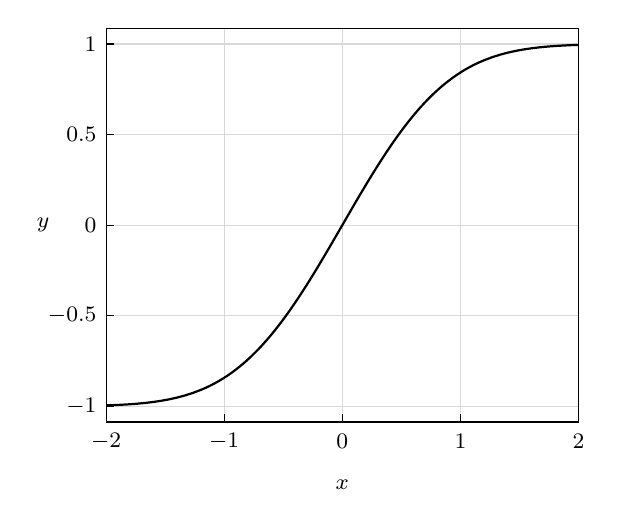
\begin{tikzpicture}
        \begin{scope}[every node/.append style = {font = \footnotesize}]
            \foreach \x in {-2, ..., 2}
                \node at (3*\x/2,-2.75) {$\x$};
            \foreach \x in {-1, 0, 1} {
                \draw[style = thin, gray!30!white] (3*\x/2,-2.5) -- (3*\x/2,2.5);
                \draw (3*\x/2,-2.5) -- (3*\x/2,-2.4);
            }
            \foreach \y in {-1, -0.5, ..., 1} {
                \node[anchor = east] at (-3,2.3*\y) {$\y$};
                \draw[style = thin, gray!30!white] (-3,2.3*\y) -- (3,2.3*\y);
                \draw (-3,2.3*\y) -- (-2.9,2.3*\y);
            }
            \node at (0,-3.3) {$x$};
            \node at (-3.8,0) {$y$};
        \end{scope}
        \begin{scope}
        \draw[clip] (-3,-2.5) -- (3,-2.5) -- (3,2.5) -- (-3,2.5) -- cycle;
        \draw[style = thick] plot[smooth, tension = 0.7] coordinates{(-3,-2.28924) (-2.9,-2.28562) (-2.8,-2.28092) (-2.7,-2.27491) (-2.6,-2.26726) (-2.5,-2.25763) (-2.4,-2.2456) (-2.3,-2.23072) (-2.2,-2.21246) (-2.1,-2.19026) (-2,-2.1635) (-1.9,-2.13155) (-1.8,-2.09372) (-1.7,-2.04934) (-1.6,-1.99772) (-1.5,-1.93821) (-1.4,-1.87023) (-1.3,-1.79324) (-1.2,-1.70683) (-1.1,-1.6107) (-1,-1.50471) (-0.9,-1.38887) (-0.8,-1.26339) (-0.7,-1.12867) (-0.6,-0.985302) (-0.5,-0.834091) (-0.4,-0.676012) (-0.3,-0.512216) (-0.2,-0.343997) (-0.1,-0.172762) (0,0.) (0.1,0.172762) (0.2,0.343997) (0.3,0.512216) (0.4,0.676012) (0.5,0.834091) (0.6,0.985302) (0.7,1.12867) (0.8,1.26339) (0.9,1.38887) (1,1.50471) (1.1,1.6107) (1.2,1.70683) (1.3,1.79324) (1.4,1.87023) (1.5,1.93821) (1.6,1.99772) (1.7,2.04934) (1.8,2.09372) (1.9,2.13155) (2,2.1635) (2.1,2.19026) (2.2,2.21246) (2.3,2.23072) (2.4,2.2456) (2.5,2.25763) (2.6,2.26726) (2.7,2.27491) (2.8,2.28092) (2.9,2.28562) (3,2.28924)};
        \end{scope}
    \end{tikzpicture}
\end{figure}

\begin{figure}[!ht]
    \makebox[\linewidth][c] {
        \centering
        \subfigure{
            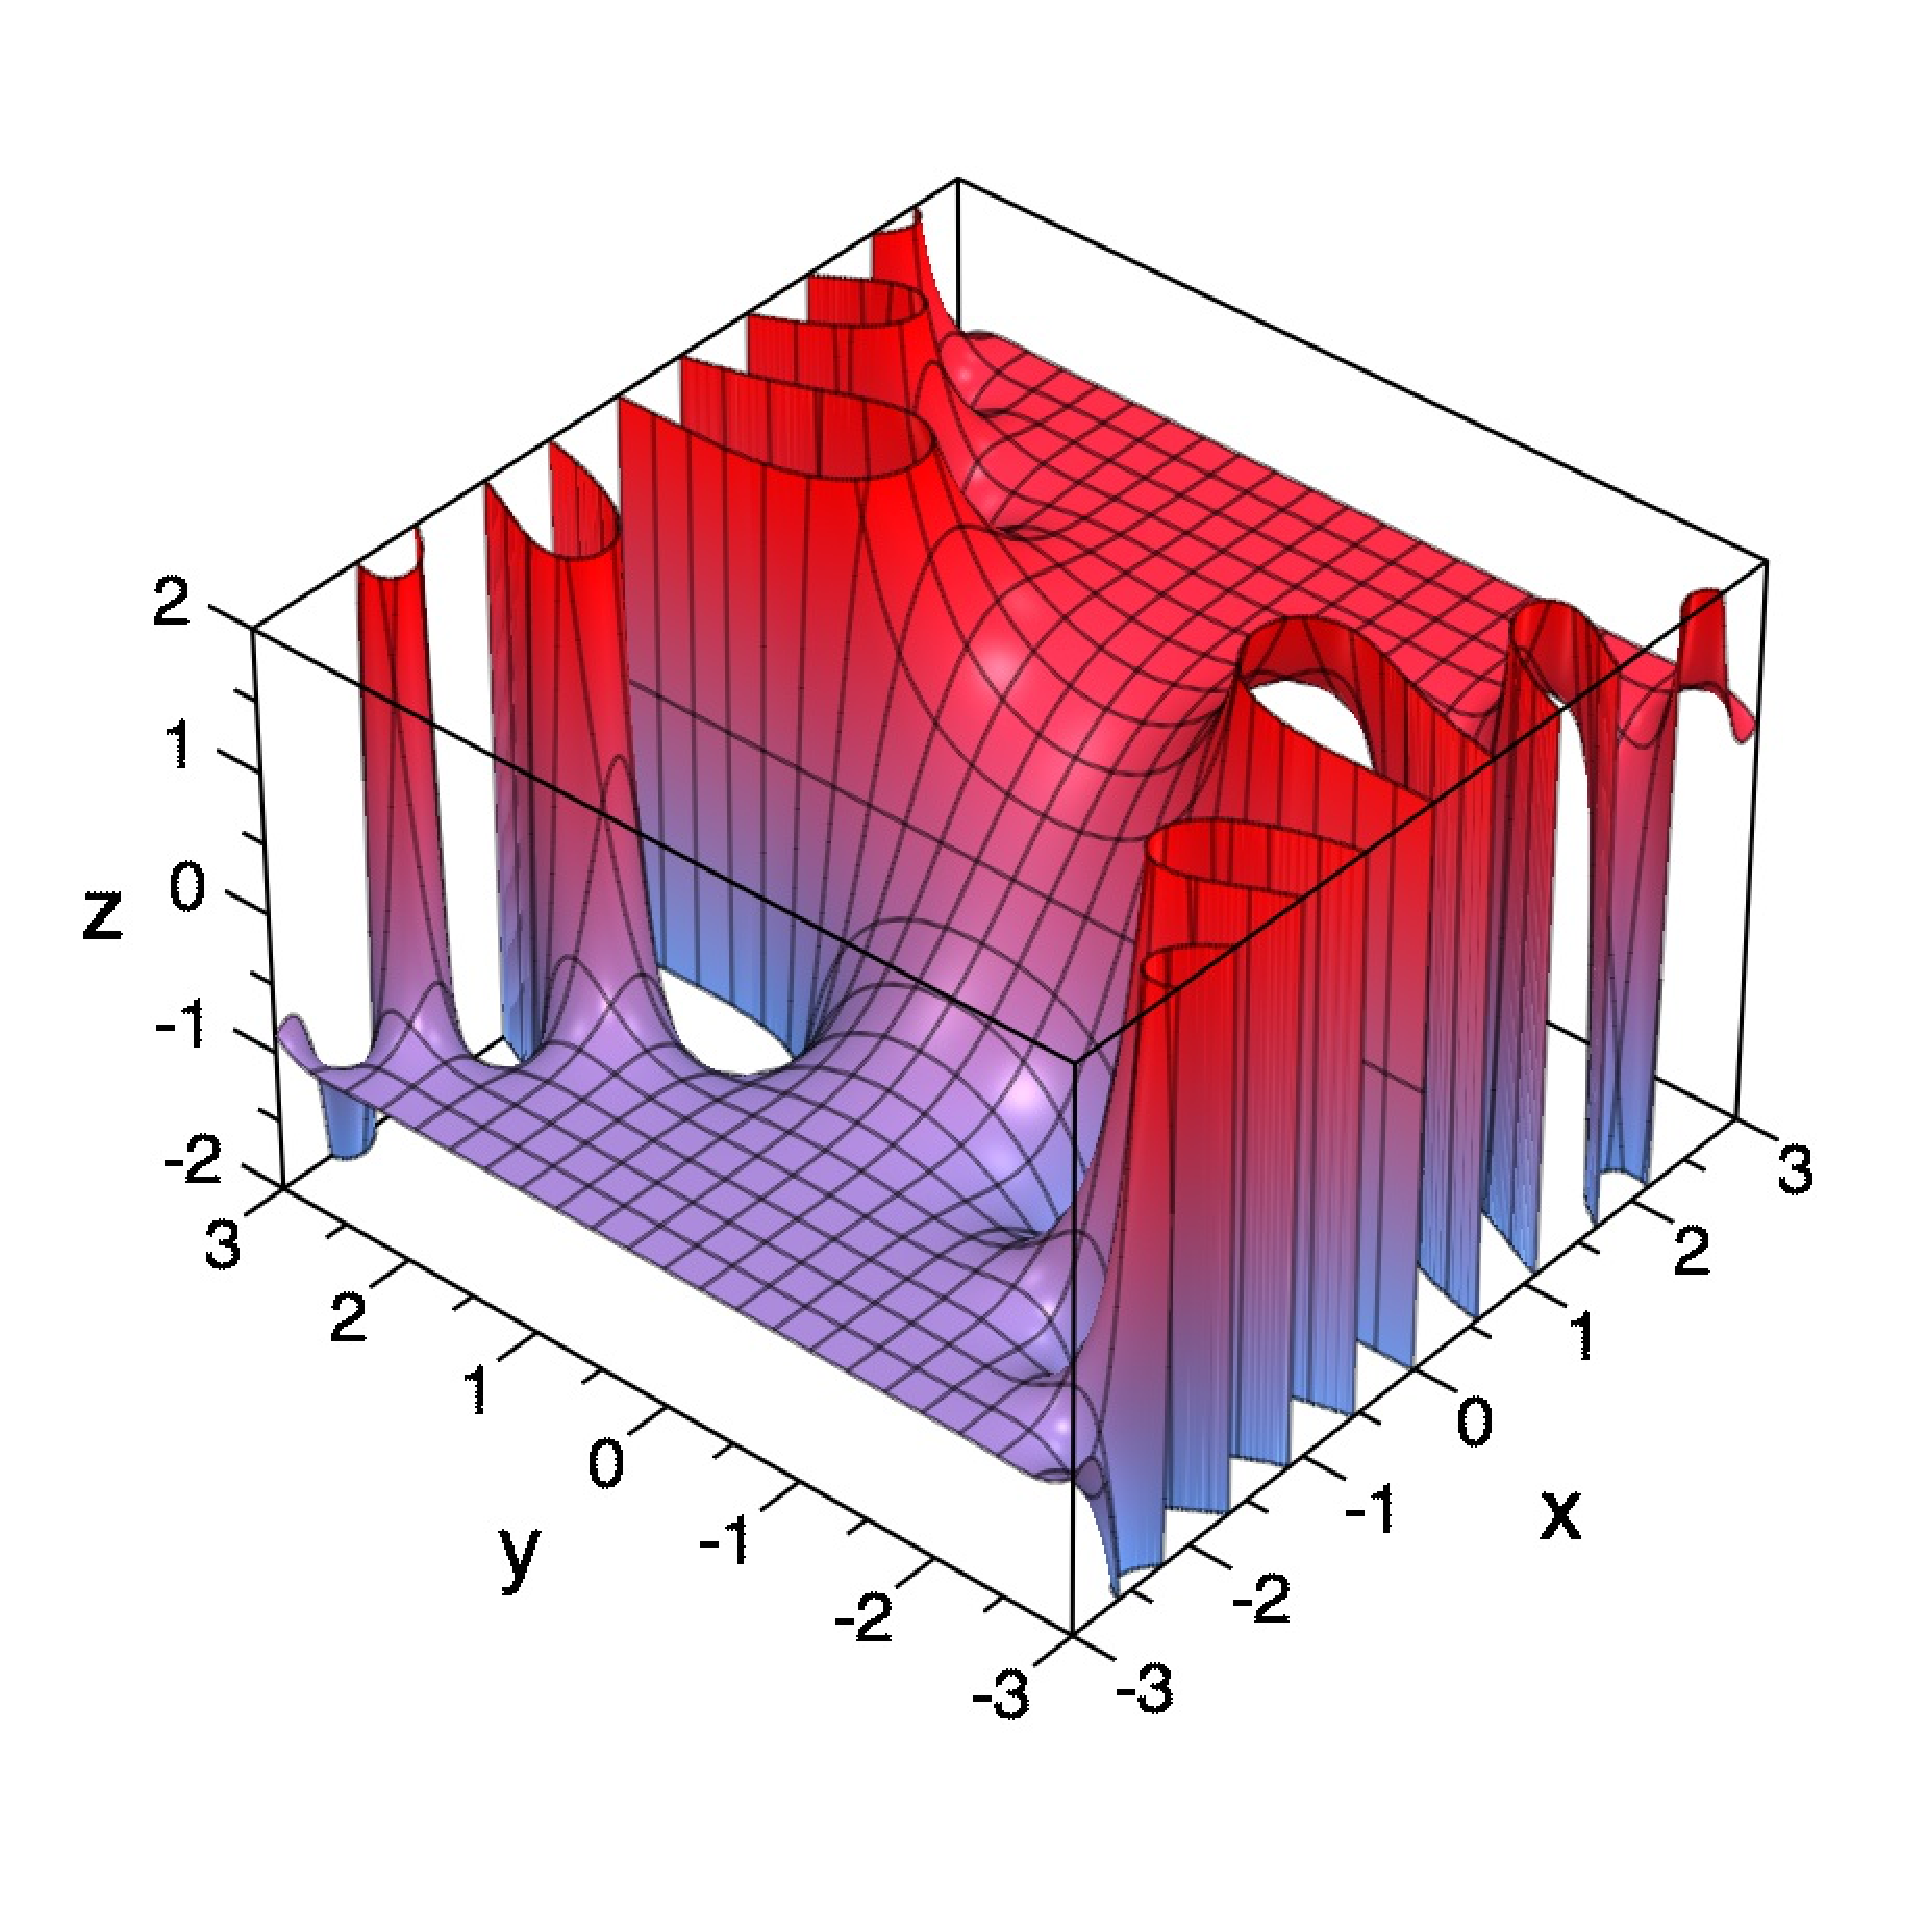
\includegraphics[width = 0.45\textwidth]{ErfFuncRe.eps}
        }
        \subfigure{
            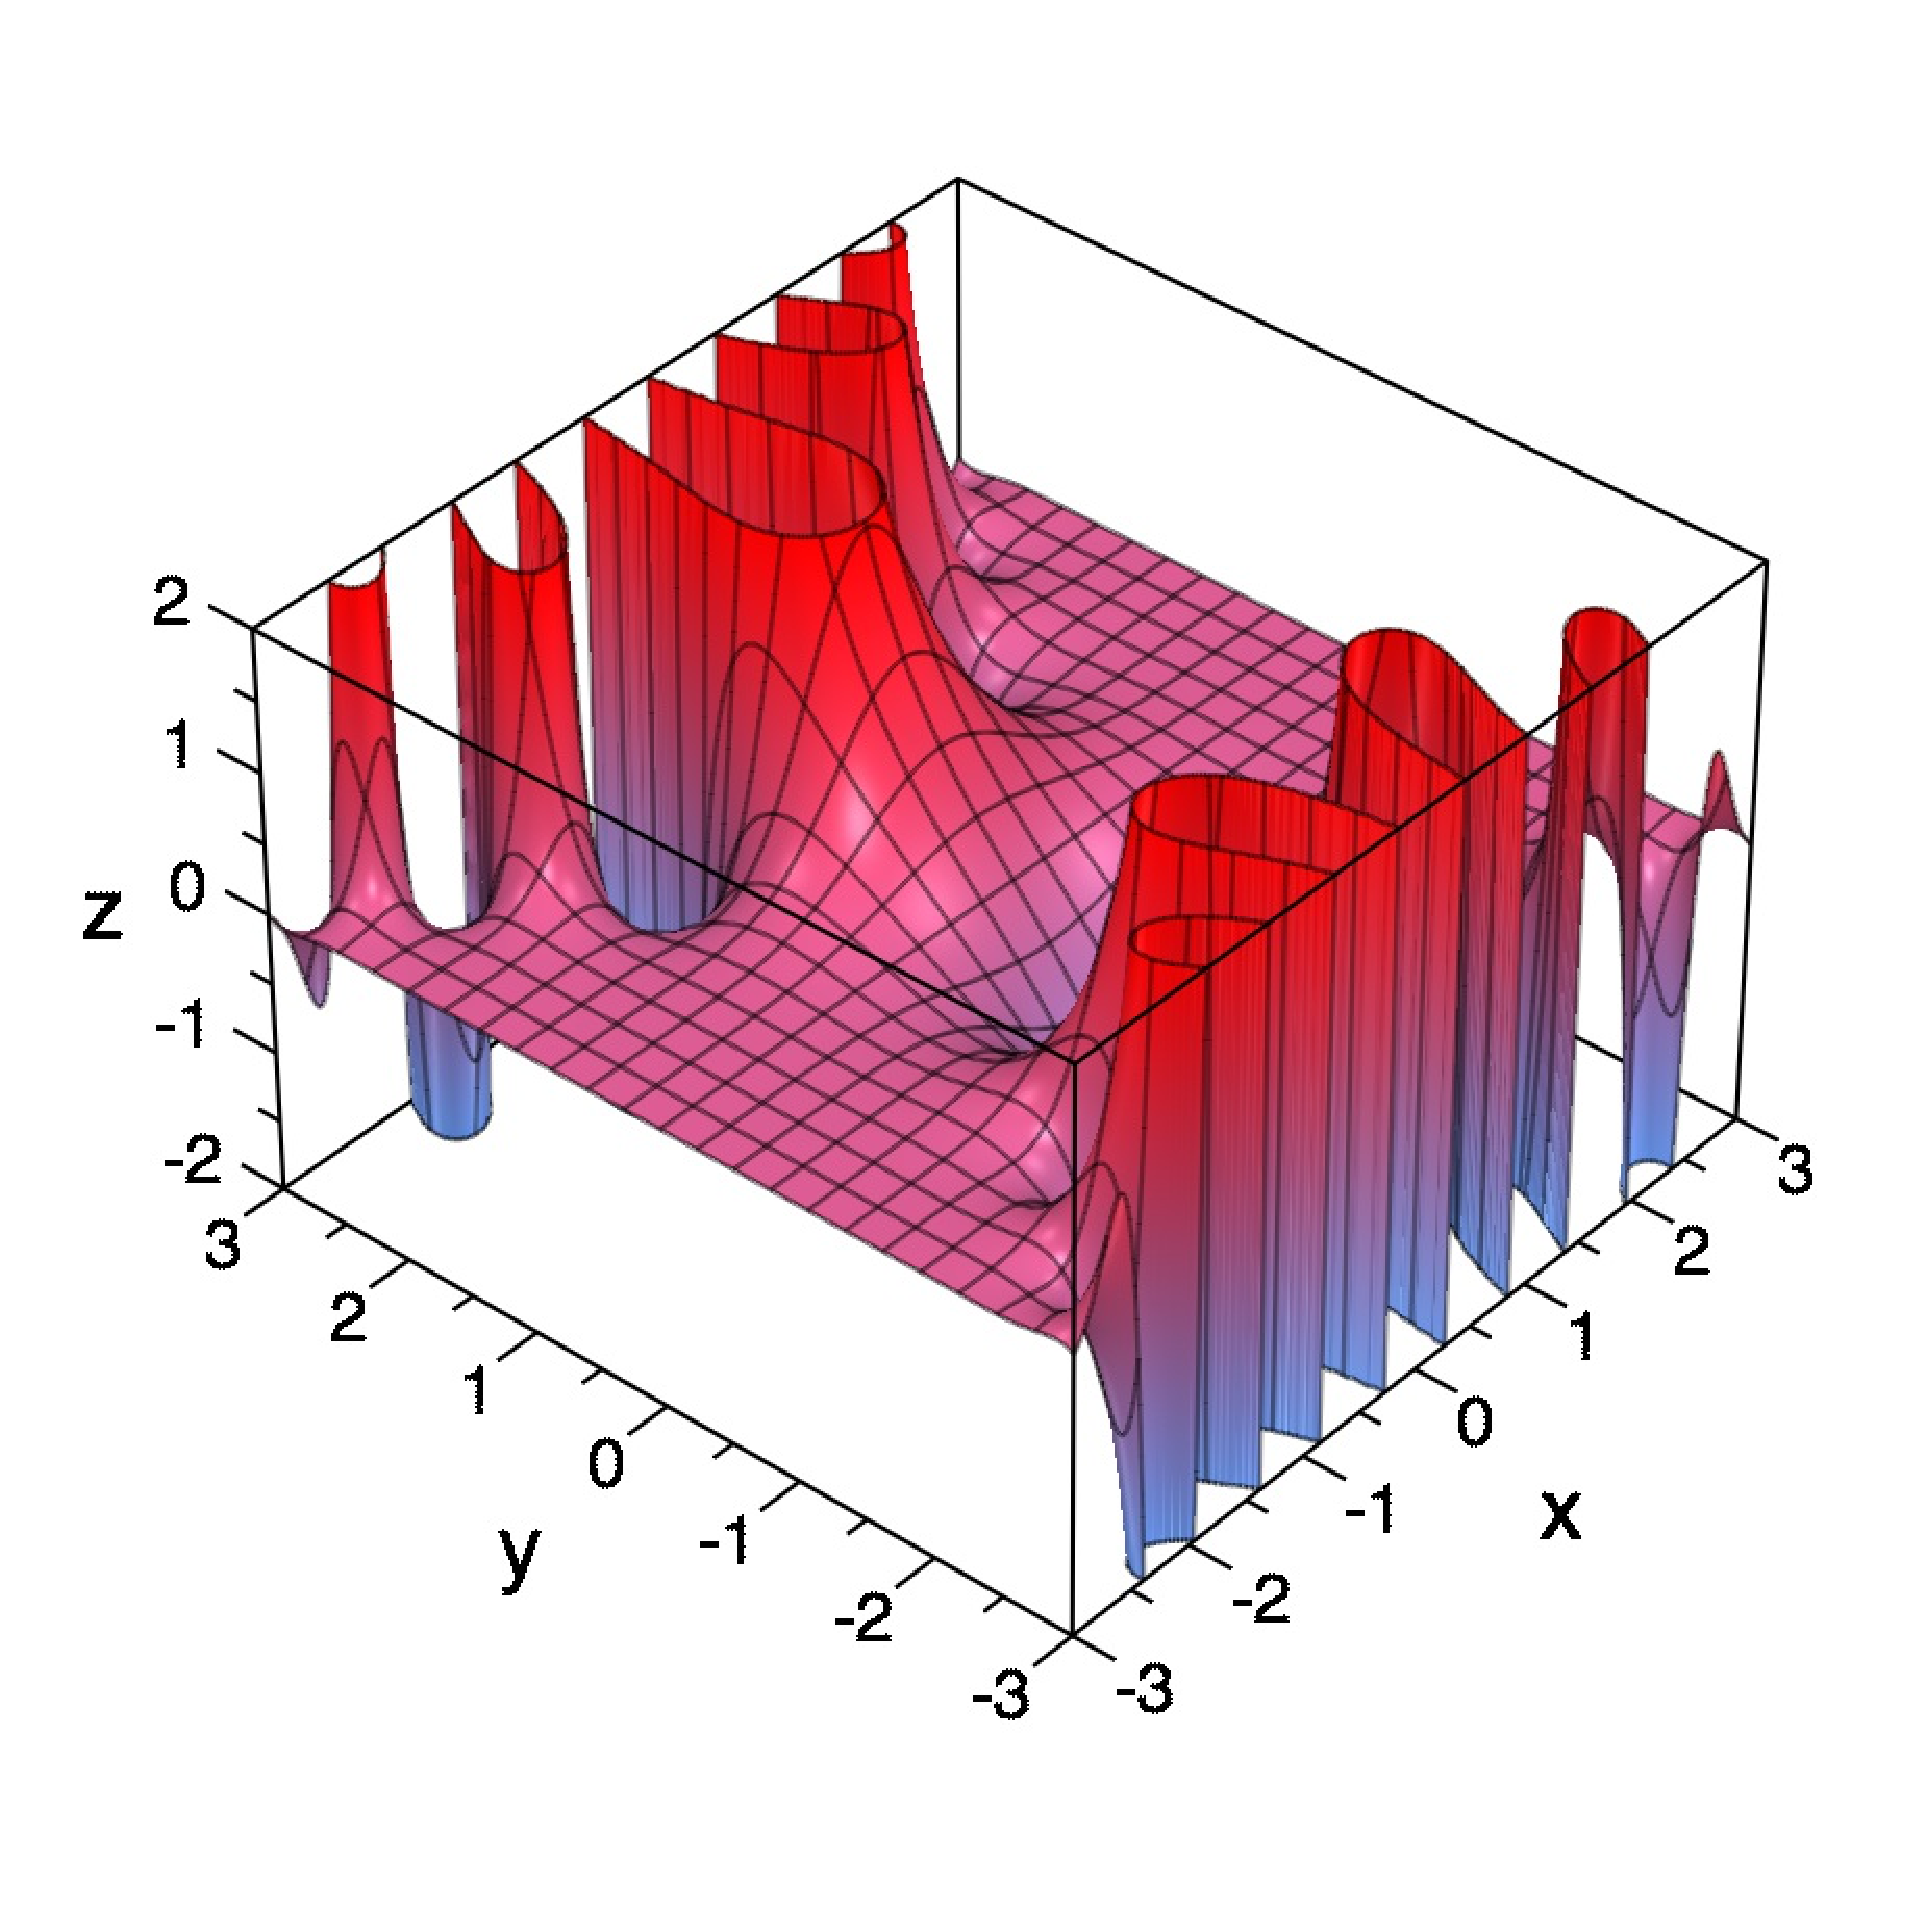
\includegraphics[width = 0.45\textwidth]{ErfFuncIm.eps}
        }
        \subfigure{
            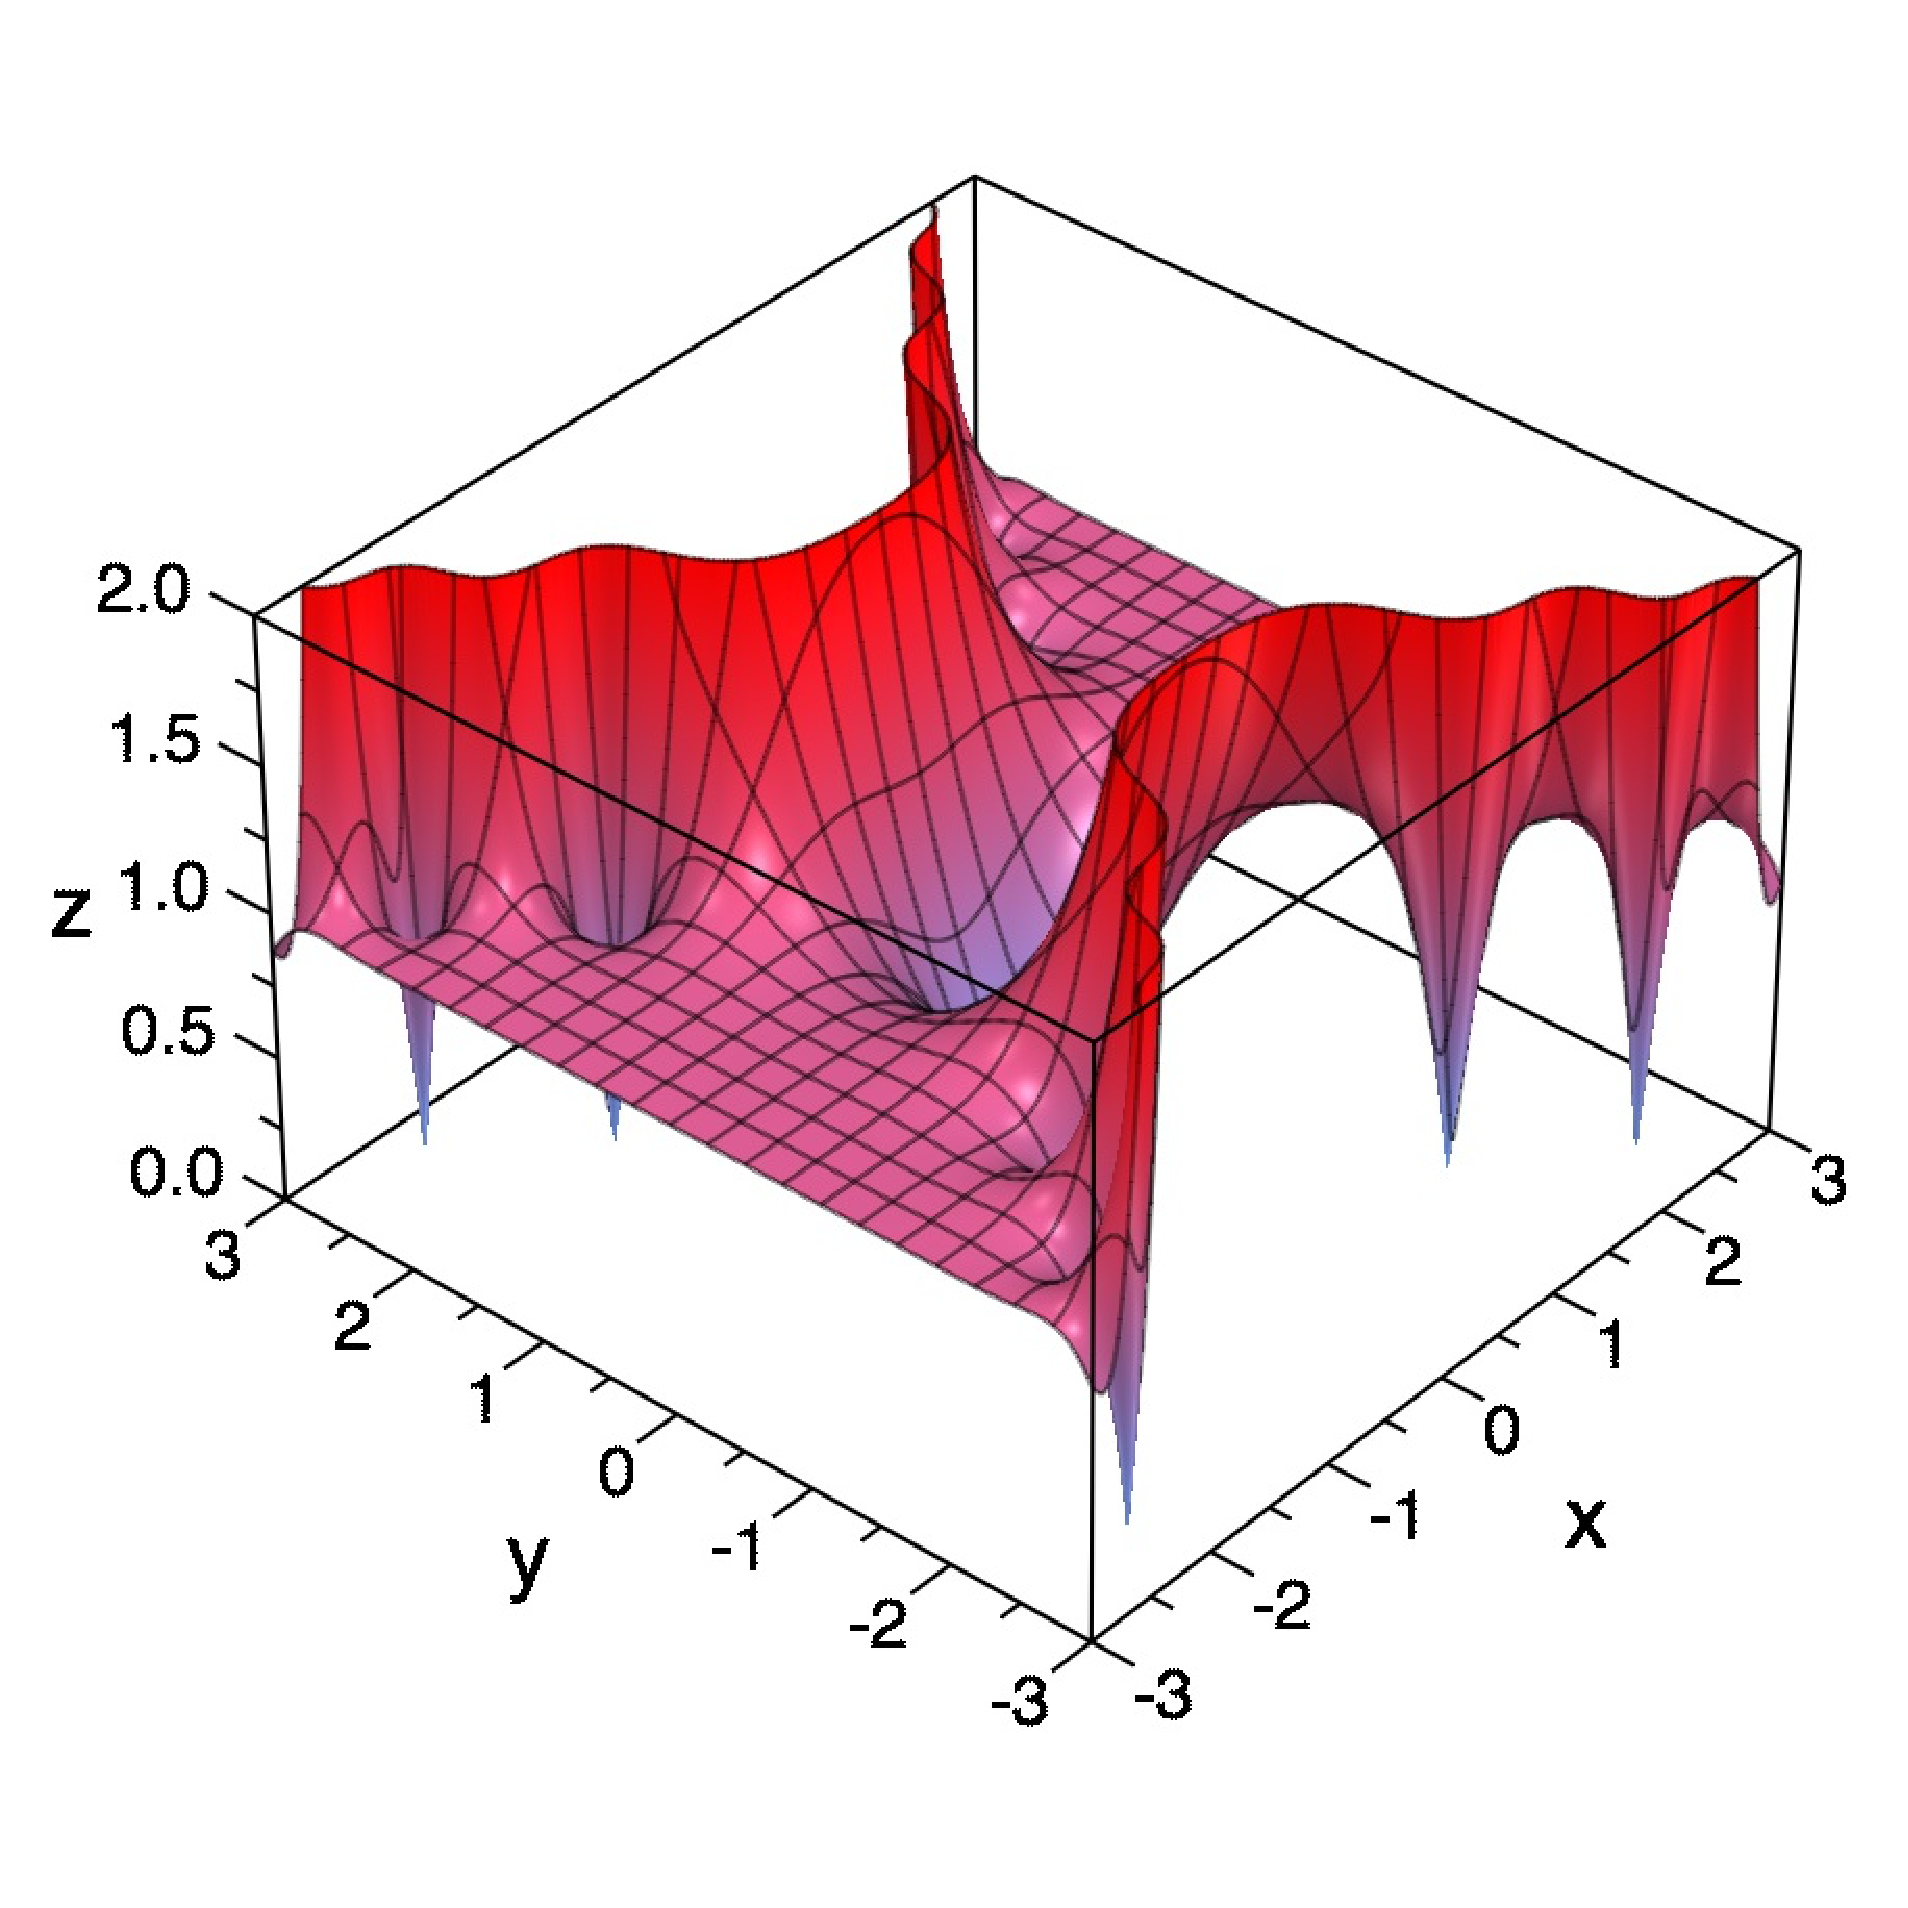
\includegraphics[width = 0.45\textwidth]{ErfFuncAbs.eps}
        }
    }
    \caption{오차함수 $y=\erf(x)$의 그래프. (위) 한편, 대부분의 특수함수들이 그러하듯, 오차함수는 그 정의역을 $\mathbb{C}$로 자연스럽게 확장할 수 있다. 물론, 본문에서 이에 대해 자세히 설명하지 않았으므로 이 책에서 이런 사실이 사용되지는 않겠지만, 참고삼아 $z=\re(\erf(x+y\imag))$ (왼쪽 아래), $z=\im(\erf(x+y\imag))$ (가운데 아래), $z=|\erf(x+y\imag)|$ (오른쪽 아래)의 그래프를 실었다. (Rendered by MATLAB Symbolic Math Toolbox MuPAD.)}
\end{figure}

여기서 오차함수가 well-define되는지, 즉 임의의 $x\in\mathbb{R}$에 대해 위의 정의의 적분이 항상 유한한가를 확인해야 하는데, 이는 다음을 보이는 것으로 충분하다. 정리라고 하기도 조금 어색한 이 정적분은 하도 유명한 나머지 무려 Gauss 적분이라는 거창한 이름도 붙어 있으며 앞으로도 잊을만 하면 계속 튀어나오므로 그 결과도 기억해 두면 좋다. 아마 고등학생 시절 수학에 관심이 있었다면 어디에선가 정적분을 구하는 신박한 방법 중 하나로 접한 기억이 있을수도 있다.

\begin{theorem}[Gauss integral]
    \begin{equation*}
        \int_0^\infty e^{-x^2}\,dx=\frac{\sqrt{\pi}}{2}
    \end{equation*}
\end{theorem}

\begin{proof}
    구하고자 하는 적분을 $I$라 하면 극좌표 변환을 통해
    \begin{align*}
        I^2&=\int_{\mathbb{R}^2}e^{-(x^2+y^2)}\,dx\,dy\\
        &=\int_0^{\pi/2}\int_0^\infty e^{-r^2}r\,dr\,d\theta\\
        &=\int_0^{\pi/2}\bigg[-\frac{1}{2}e^{-r^2}\bigg]_0^\infty\,d\theta\\
        &=\int_0^{\pi/2}\frac{1}{2}\,d\theta\\
        &=\frac{\pi}{4}
    \end{align*}
    임을 안다.
\end{proof}

\subsection{Gamma Function}

다음으로 알아볼 함수는 감마함수이다.

\begin{definition}
    다음과 같이 정의되는 함수 $\Gamma:\mathbb{R}^+\to\mathbb{R}^+$를 \textbf{감마함수(gamma function)}라 한다.
    \begin{equation*}
        \Gamma:x\mapsto\int_0^\infty t^{x-1}e^{-t}\,dt
    \end{equation*}
\end{definition}

이번에도 감마함수가 well-define되는지 살펴보아야 하고, 이는 다음 명제를 보이는 것으로 충분하다.

\begin{proposition}
    임의의 $\alpha\in\mathbb{R}$에 대해 $I(\alpha)=\int_0^\infty x^{\alpha-1}e^{-x}\,dx$라 하면 $\alpha>0$일때 $I(\alpha)<\infty$이고, 그렇지 않으면 $I(\alpha)=\infty$이다.
\end{proposition}

\begin{proof}
    먼저 $\alpha>0$인 경우를 생각하면 적당한 $M>0$이 존재하여 $x\geq M$이면 $x^{\alpha-1}<e^{x/2}$이므로 $\int_1^\infty x^{\alpha-1}e^{-x}\,dx\leq\int_1^Mx^{\alpha-1}e^{-x}\,dx+\int_M^\infty e^{-x/2}\,dx=\int_1^Mx^{\alpha-1}e^{-x}\,dx+2e^{-M/2}<\infty$이다. 따라서 $\int_0^1x^{\alpha-1}e^{-x}\,dx<\infty$임을 보이면 이 경우에 대해서는 충분한데, 여기서 $\alpha\geq1$이면 피적분함수 $x^{\alpha-1}e^{-x}$가 $[0,\,1]$에서 유계이므로 $\int_0^1x^{\alpha-1}e^{-x}\,dx<\infty$이고, $0<\alpha<1$이라도 $\int_0^1x^{\alpha-1}e^{-x}\,dx\leq\int_0^1x^{\alpha-1}\,dx=[x^\alpha/\alpha]_0^1=1/\alpha<\infty$이므로 곧 $\alpha>0$이면 $I(\alpha)<\infty$이다. 한편, $\alpha\leq0$인 경우에는 모든 $x\in\mathbb{R}$에 대해 $e^{-x}\geq1-x$이므로 $I(\alpha)\geq\int_0^1x^{\alpha-1}e^{-x}\,dx\geq\int_0^1e^{-x}/x\,dx\geq\int_0^1(1-x)/x\,dx=[\log x-x]_0^1=\infty$이다.
\end{proof}

\begin{figure}[!ht]
    \centering
    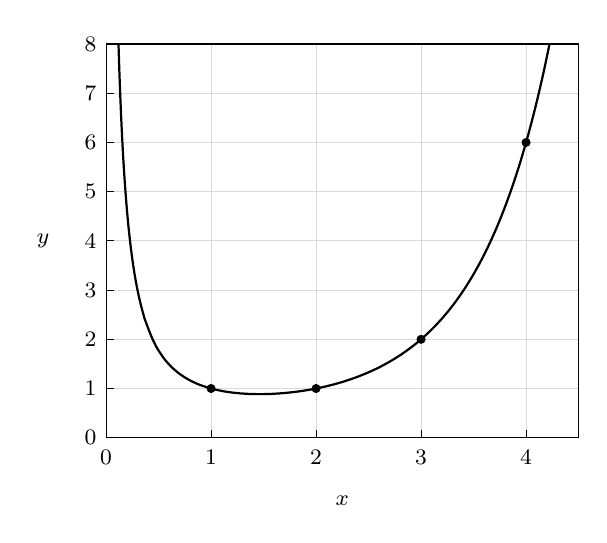
\begin{tikzpicture}
        \begin{scope}[every node/.append style = {font = \footnotesize}]
            \foreach \x in {0, ..., 4}
                \node at (6*\x/4.5,-0.25) {$\x$};
            \foreach \x in {1, ..., 4} {
                \draw[style = thin, gray!30!white] (6*\x/4.5,0) -- (6*\x/4.5,5);
                \draw (6*\x/4.5,0) -- (6*\x/4.5,0.1);
            }
            \foreach \y in {0, ..., 8} {
                \node[anchor = east] at (0,5*\y/8) {$\y$};
                \draw[style = thin, gray!30!white] (0,5*\y/8) -- (6,5*\y/8);
                \draw (0,5*\y/8) -- (0.1,5*\y/8);
            }
            \node at (3,-0.8) {$x$};
            \node at (-0.8,2.5) {$y$};
        \end{scope}
        \begin{scope}
        \draw[clip] (0,0) -- (6,0) -- (6,5) -- (0,5) -- cycle;
        \draw[style = thick] plot[smooth, tension = 0.7] coordinates{(0.14,5.65092) (0.16,4.91453) (0.18,4.34331) (0.2,3.88767) (0.22,3.51604) (0.24,3.20739) (0.26,2.94715) (0.28,2.72493) (0.3,2.5331) (0.32,2.36594) (0.34,2.21908) (0.36,2.08913) (0.38,1.97339) (0.4,1.86973) (0.42,1.77641) (0.44,1.692) (0.46,1.61535) (0.48,1.54546) (0.5,1.48152) (0.6,1.23009) (0.7,1.0563) (0.8,0.930745) (0.9,0.837166) (1,0.765885) (1.1,0.710802) (1.2,0.667893) (1.3,0.634414) (1.4,0.60844) (1.5,0.588589) (1.6,0.573855) (1.7,0.563498) (1.8,0.55697) (1.9,0.553866) (2,0.553892) (2.1,0.55684) (2.2,0.562573) (2.3,0.571008) (2.4,0.582115) (2.5,0.595904) (2.6,0.612425) (2.7,0.631768) (2.8,0.654054) (2.9,0.679442) (3,0.708127) (3.1,0.740341) (3.2,0.776356) (3.3,0.816486) (3.4,0.861091) (3.5,0.910583) (3.6,0.965429) (3.7,1.02616) (3.8,1.09336) (3.9,1.16772) (4,1.25) (4.1,1.34105) (4.2,1.44184) (4.3,1.55346) (4.4,1.67715) (4.5,1.81429) (4.6,1.96645) (4.7,2.1354) (4.8,2.32314) (4.9,2.53194) (5,2.76437) (5.1,3.02332) (5.2,3.31208) (5.3,3.63439) (5.4,3.99449) (5.5,4.39718) (5.6,4.84793) (5.7,5.35298)};
        \end{scope}
        \draw[fill = black] (6/4.5,5/8) circle[radius = 0.05];
        \draw[fill = black] (12/4.5,5/8) circle[radius = 0.05];
        \draw[fill = black] (18/4.5,10/8) circle[radius = 0.05];
        \draw[fill = black] (24/4.5,30/8) circle[radius = 0.05];
    \end{tikzpicture}
\end{figure}

\begin{figure}[!ht]
    \makebox[\linewidth][c]{
        \centering
        \subfigure{
            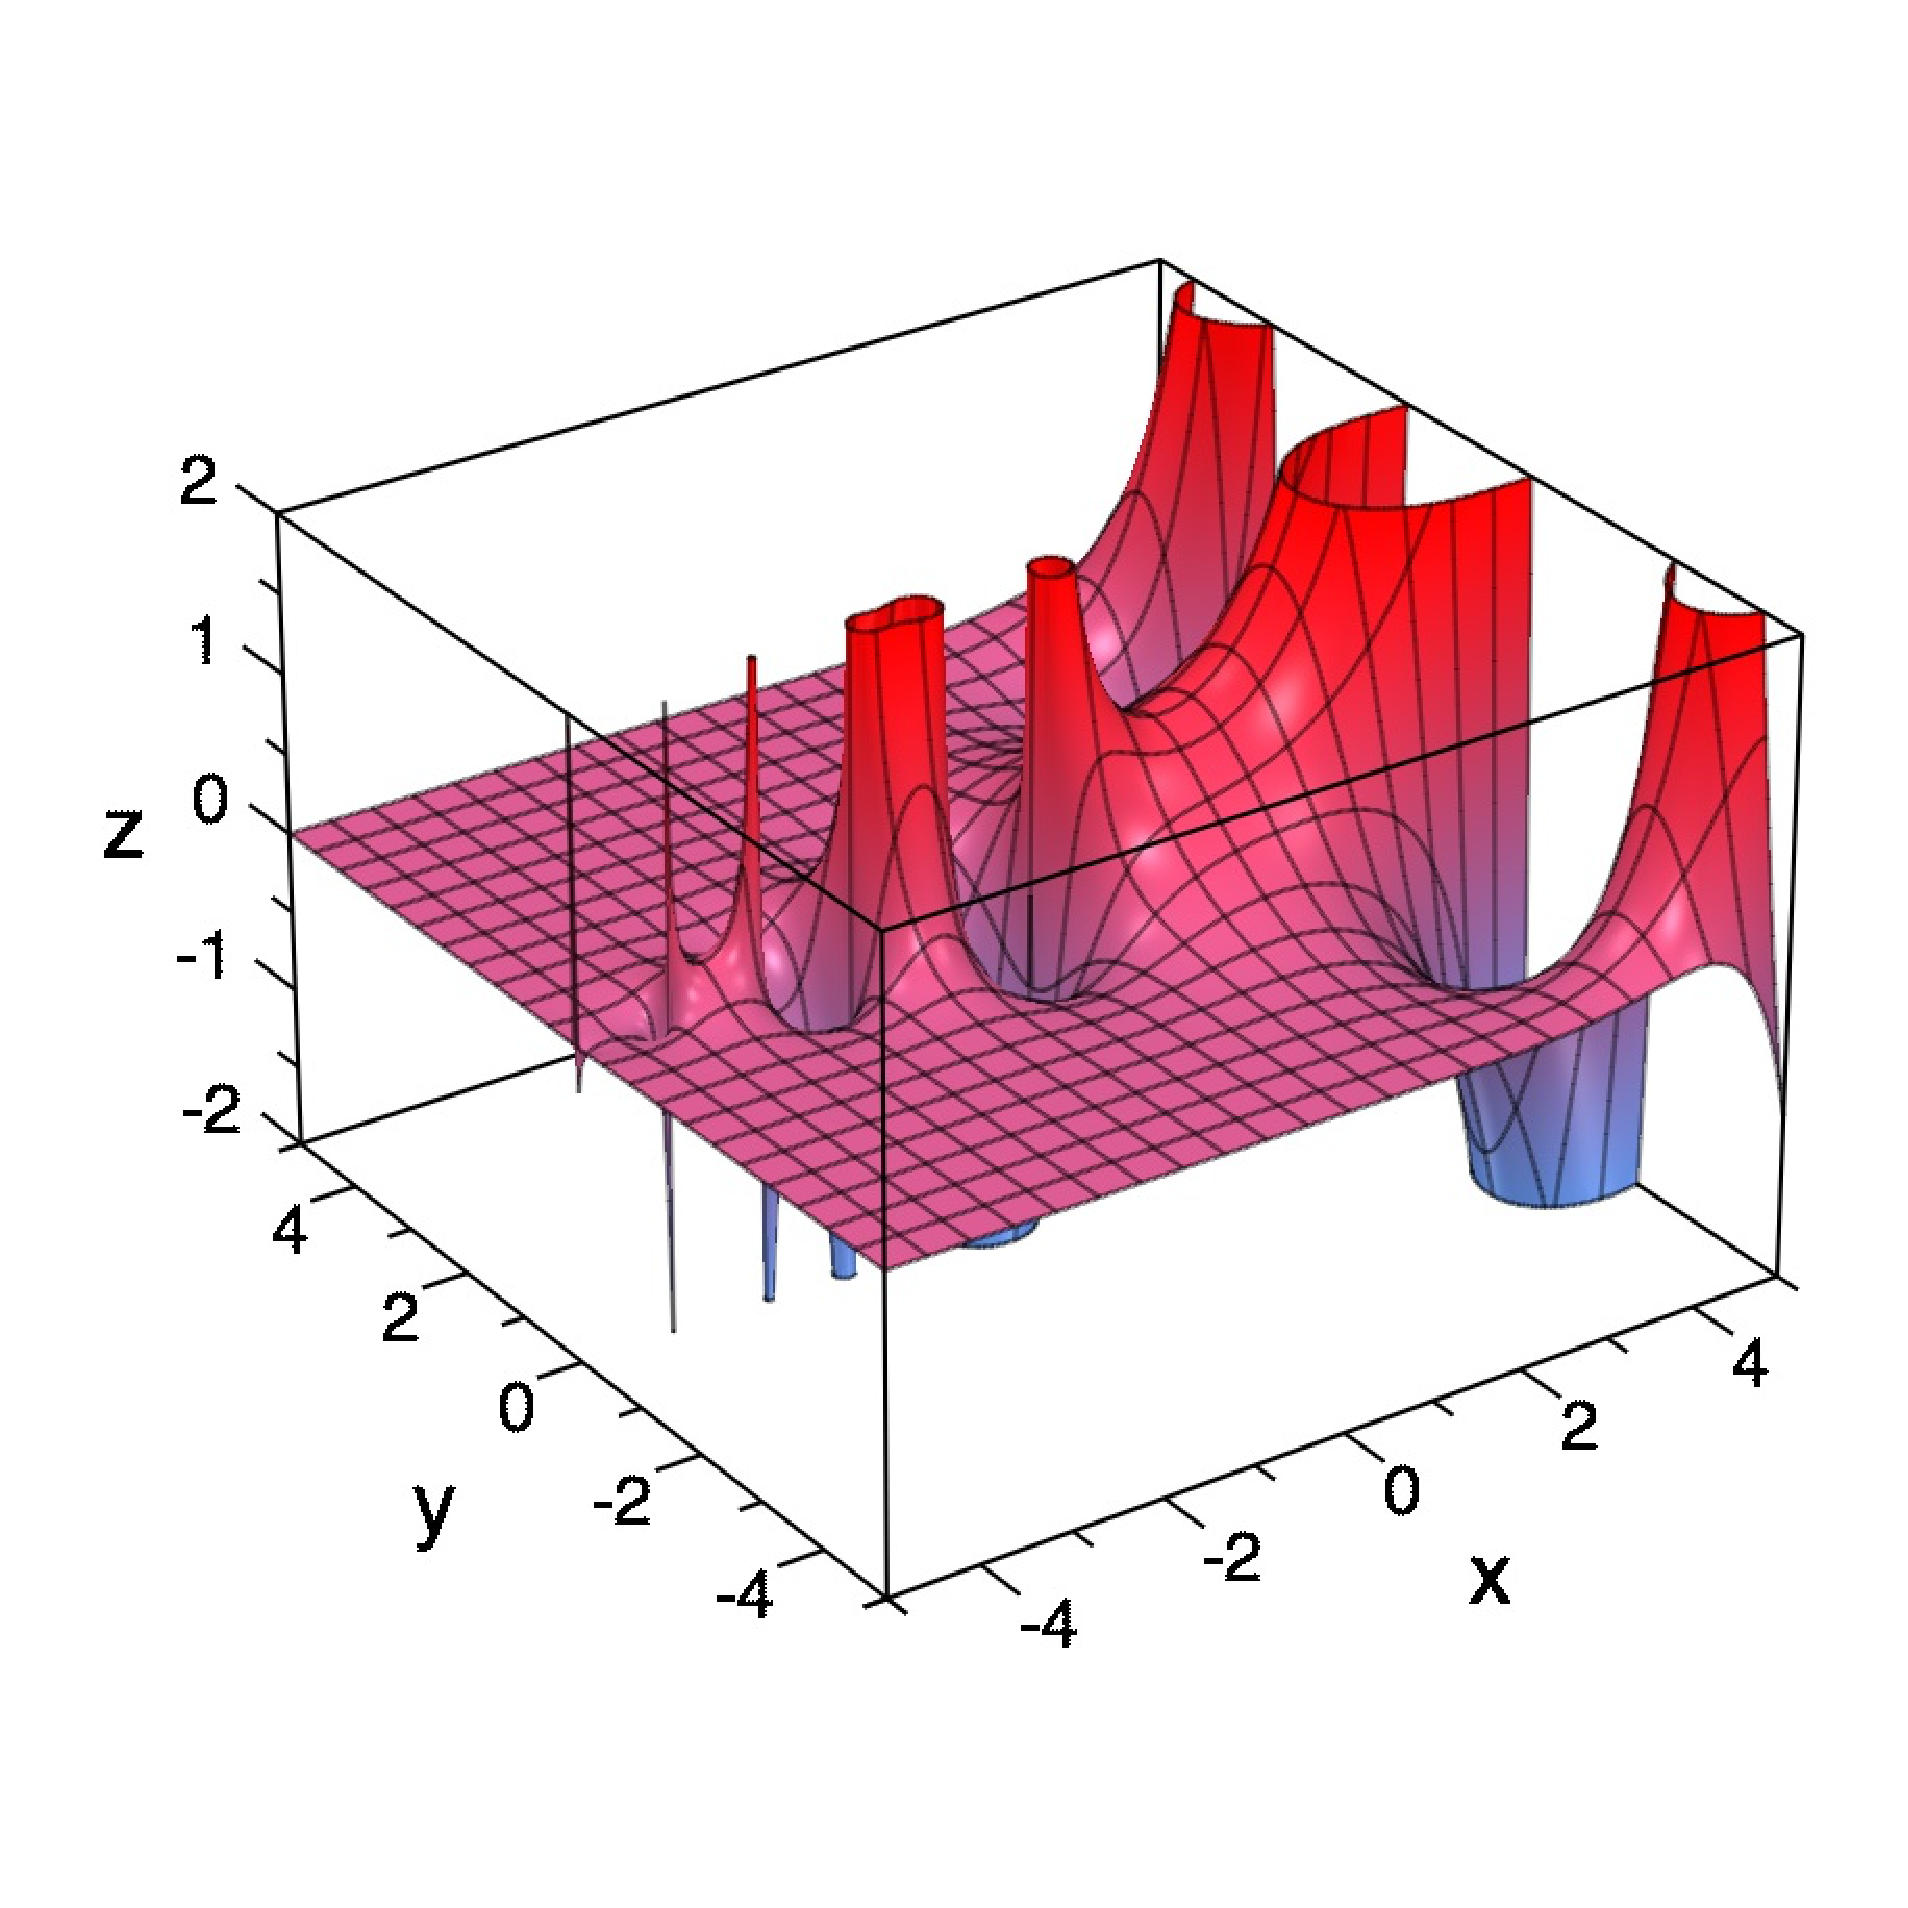
\includegraphics[width = 0.45\textwidth]{GamFuncRe.eps}
        }
        \subfigure{
            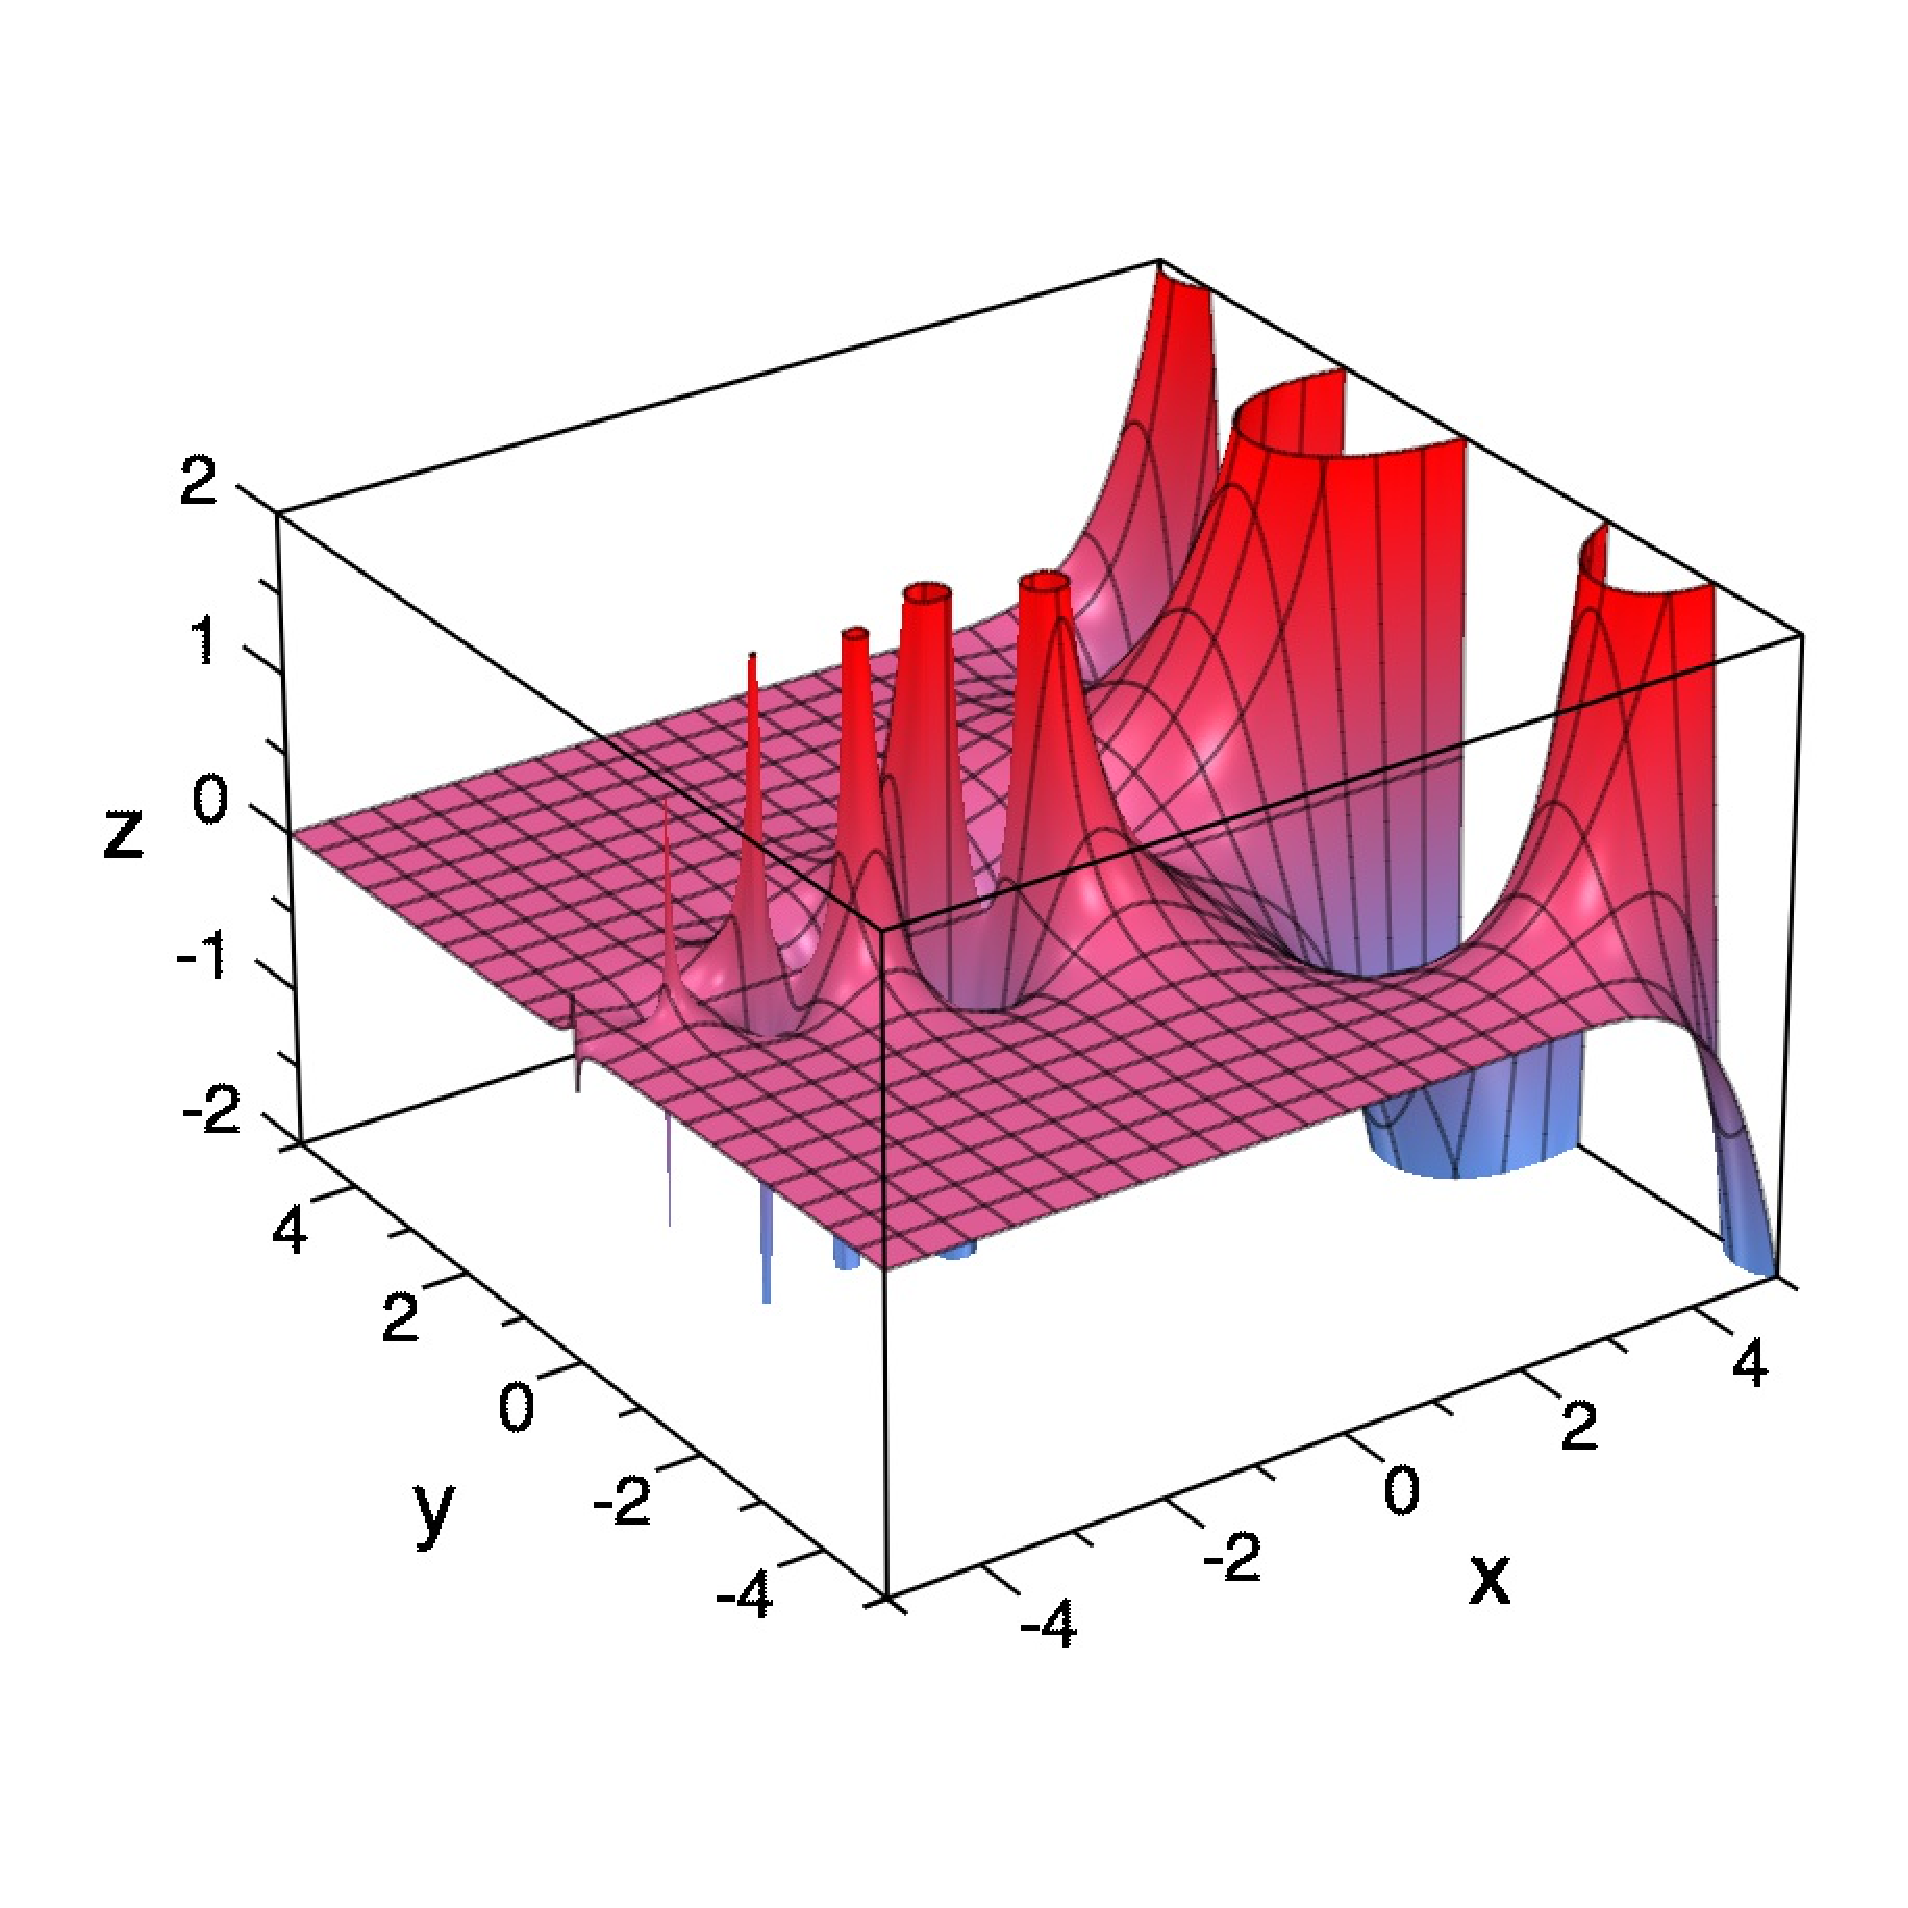
\includegraphics[width = 0.45\textwidth]{GamFuncIm.eps}
        }
        \subfigure{
            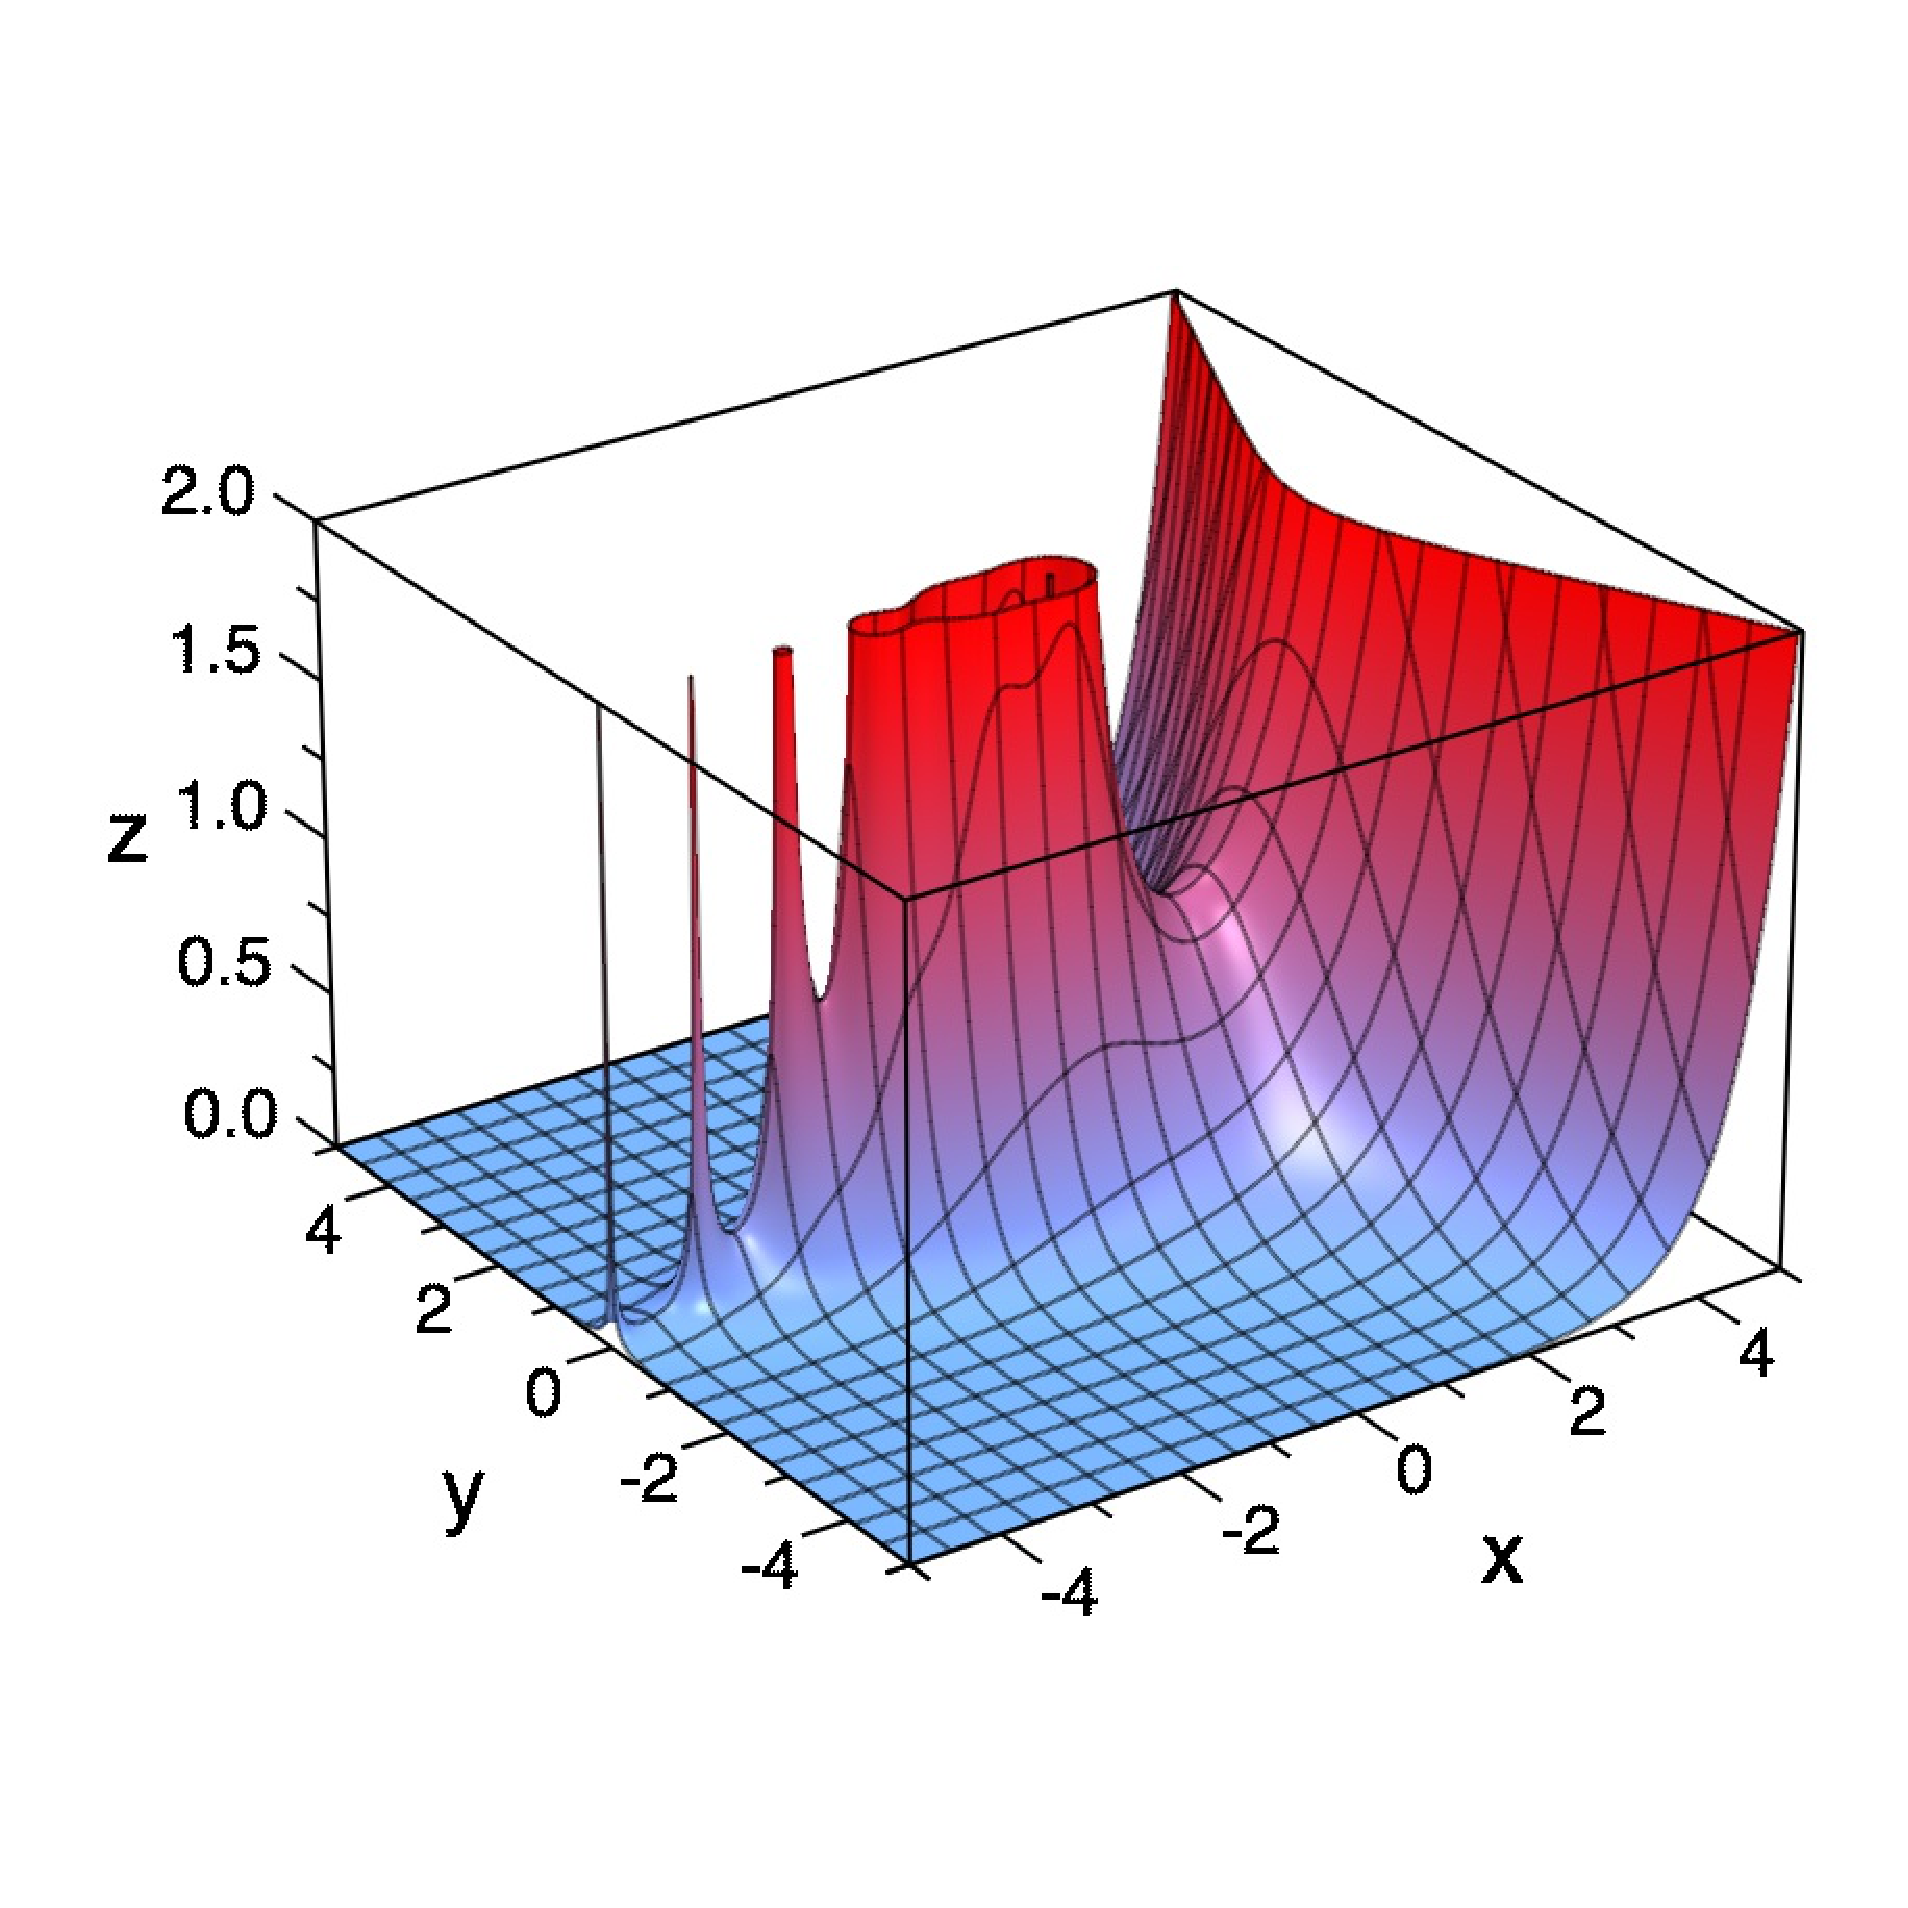
\includegraphics[width = 0.45\textwidth]{GamFuncAbs.eps}
        }
    }
    \caption{감마함수 $y=\Gamma(x)$의 그래프. (위) 한편, 감마함수도 그 정의역을 $\mathbb{C}$로 자연스럽게 확장할 수 있는데, 참고삼아 $z=\re(\Gamma(x+y\imag))$ (왼쪽 아래), $z=\im(\Gamma(x+y\imag))$ (가운데 아래), $z=|\Gamma(x+y\imag)|$ (오른쪽 아래)의 그래프를 실었다. (여기서 세 번째 그래프가 꽤나 유명하다.) 당연히 본문에는 이와 관련된 내용이 없었으므로, 이 책에서 이런 사실이 사용되지는 않을 것이다. (Rendered by MATLAB Symbolic Math Toolbox MuPAD.)}
\end{figure}

그리고 이런 감마함수로부터 파생되는 불완전 감마함수들이 있다. 그냥 이름과 정의 정도만 익혀두면 된다.

\begin{definition}
    다음과 같이 정의되는 함수 $\Gamma,\,\gamma:\mathbb{R}^+\times\mathbb{R}^+_0\to\mathbb{R}^+$를 각각 \textbf{상부 불완전 감마함수(upper incomplete gamma function), 하부 불완전 감마함수(lower incomplete gamma function)}라 한다.
    \begin{equation*}
        \Gamma:(x,\,y)\mapsto\int_y^\infty t^{x-1}e^{-t}\,dt,\qquad\gamma:(x,\,y)\mapsto\int_0^yt^{x-1}e^{-t}\,dt
    \end{equation*}
    나아가, 다음과 같이 정의되는 함수 $Q,\,P:\mathbb{R}^+\times\mathbb{R}^+_0\to\mathbb{R}^+$를 각각 \textbf{정규화된 상부 불완전 감마함수(regularized upper incomplete gamma function), 정규화된 하부 불완전 감마함수(regularized lower incomplete gamma function)}라 한다.
    \begin{equation*}
        Q:(x,\,y)\mapsto\frac{\Gamma(x,\,y)}{\Gamma(x)},\qquad P:(x,\,y)\mapsto\frac{\gamma(x,\,y)}{\Gamma(x)}
    \end{equation*}
\end{definition}

\begin{figure}[!ht]
    \centering
    \subfigure{
        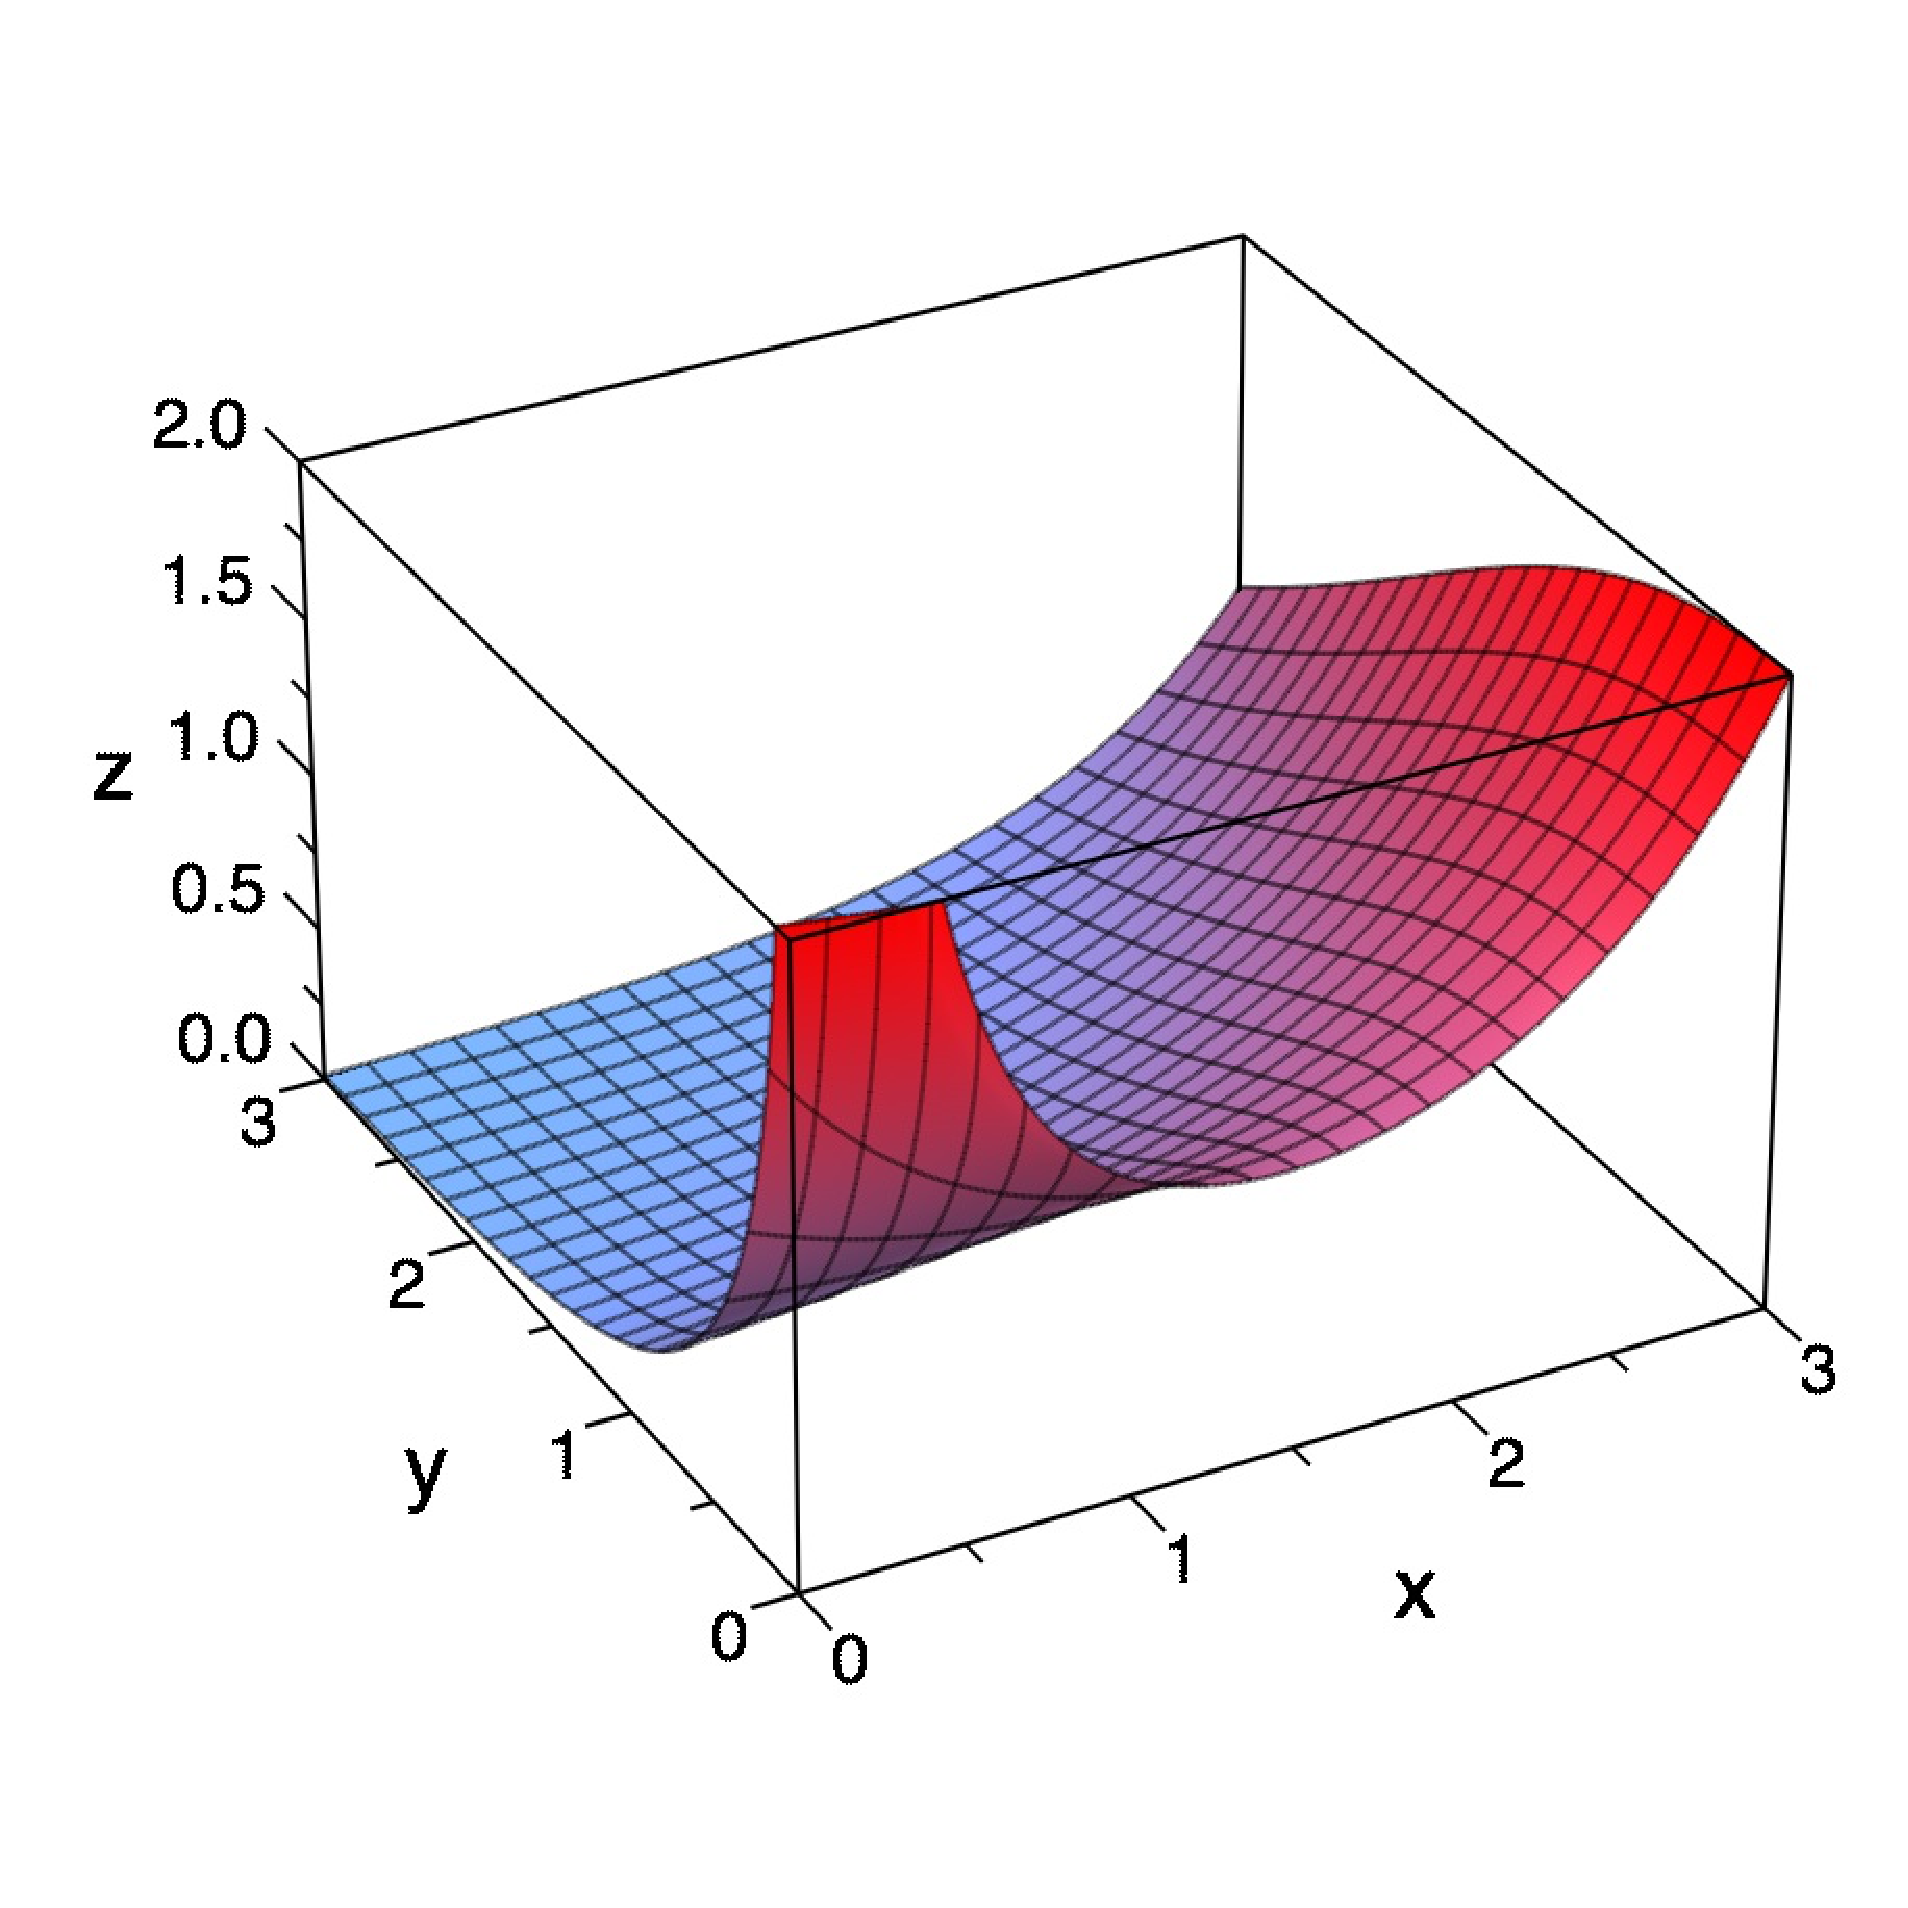
\includegraphics[width = 0.45\textwidth]{UppIncGamFunc.eps}
    }
    \subfigure{
        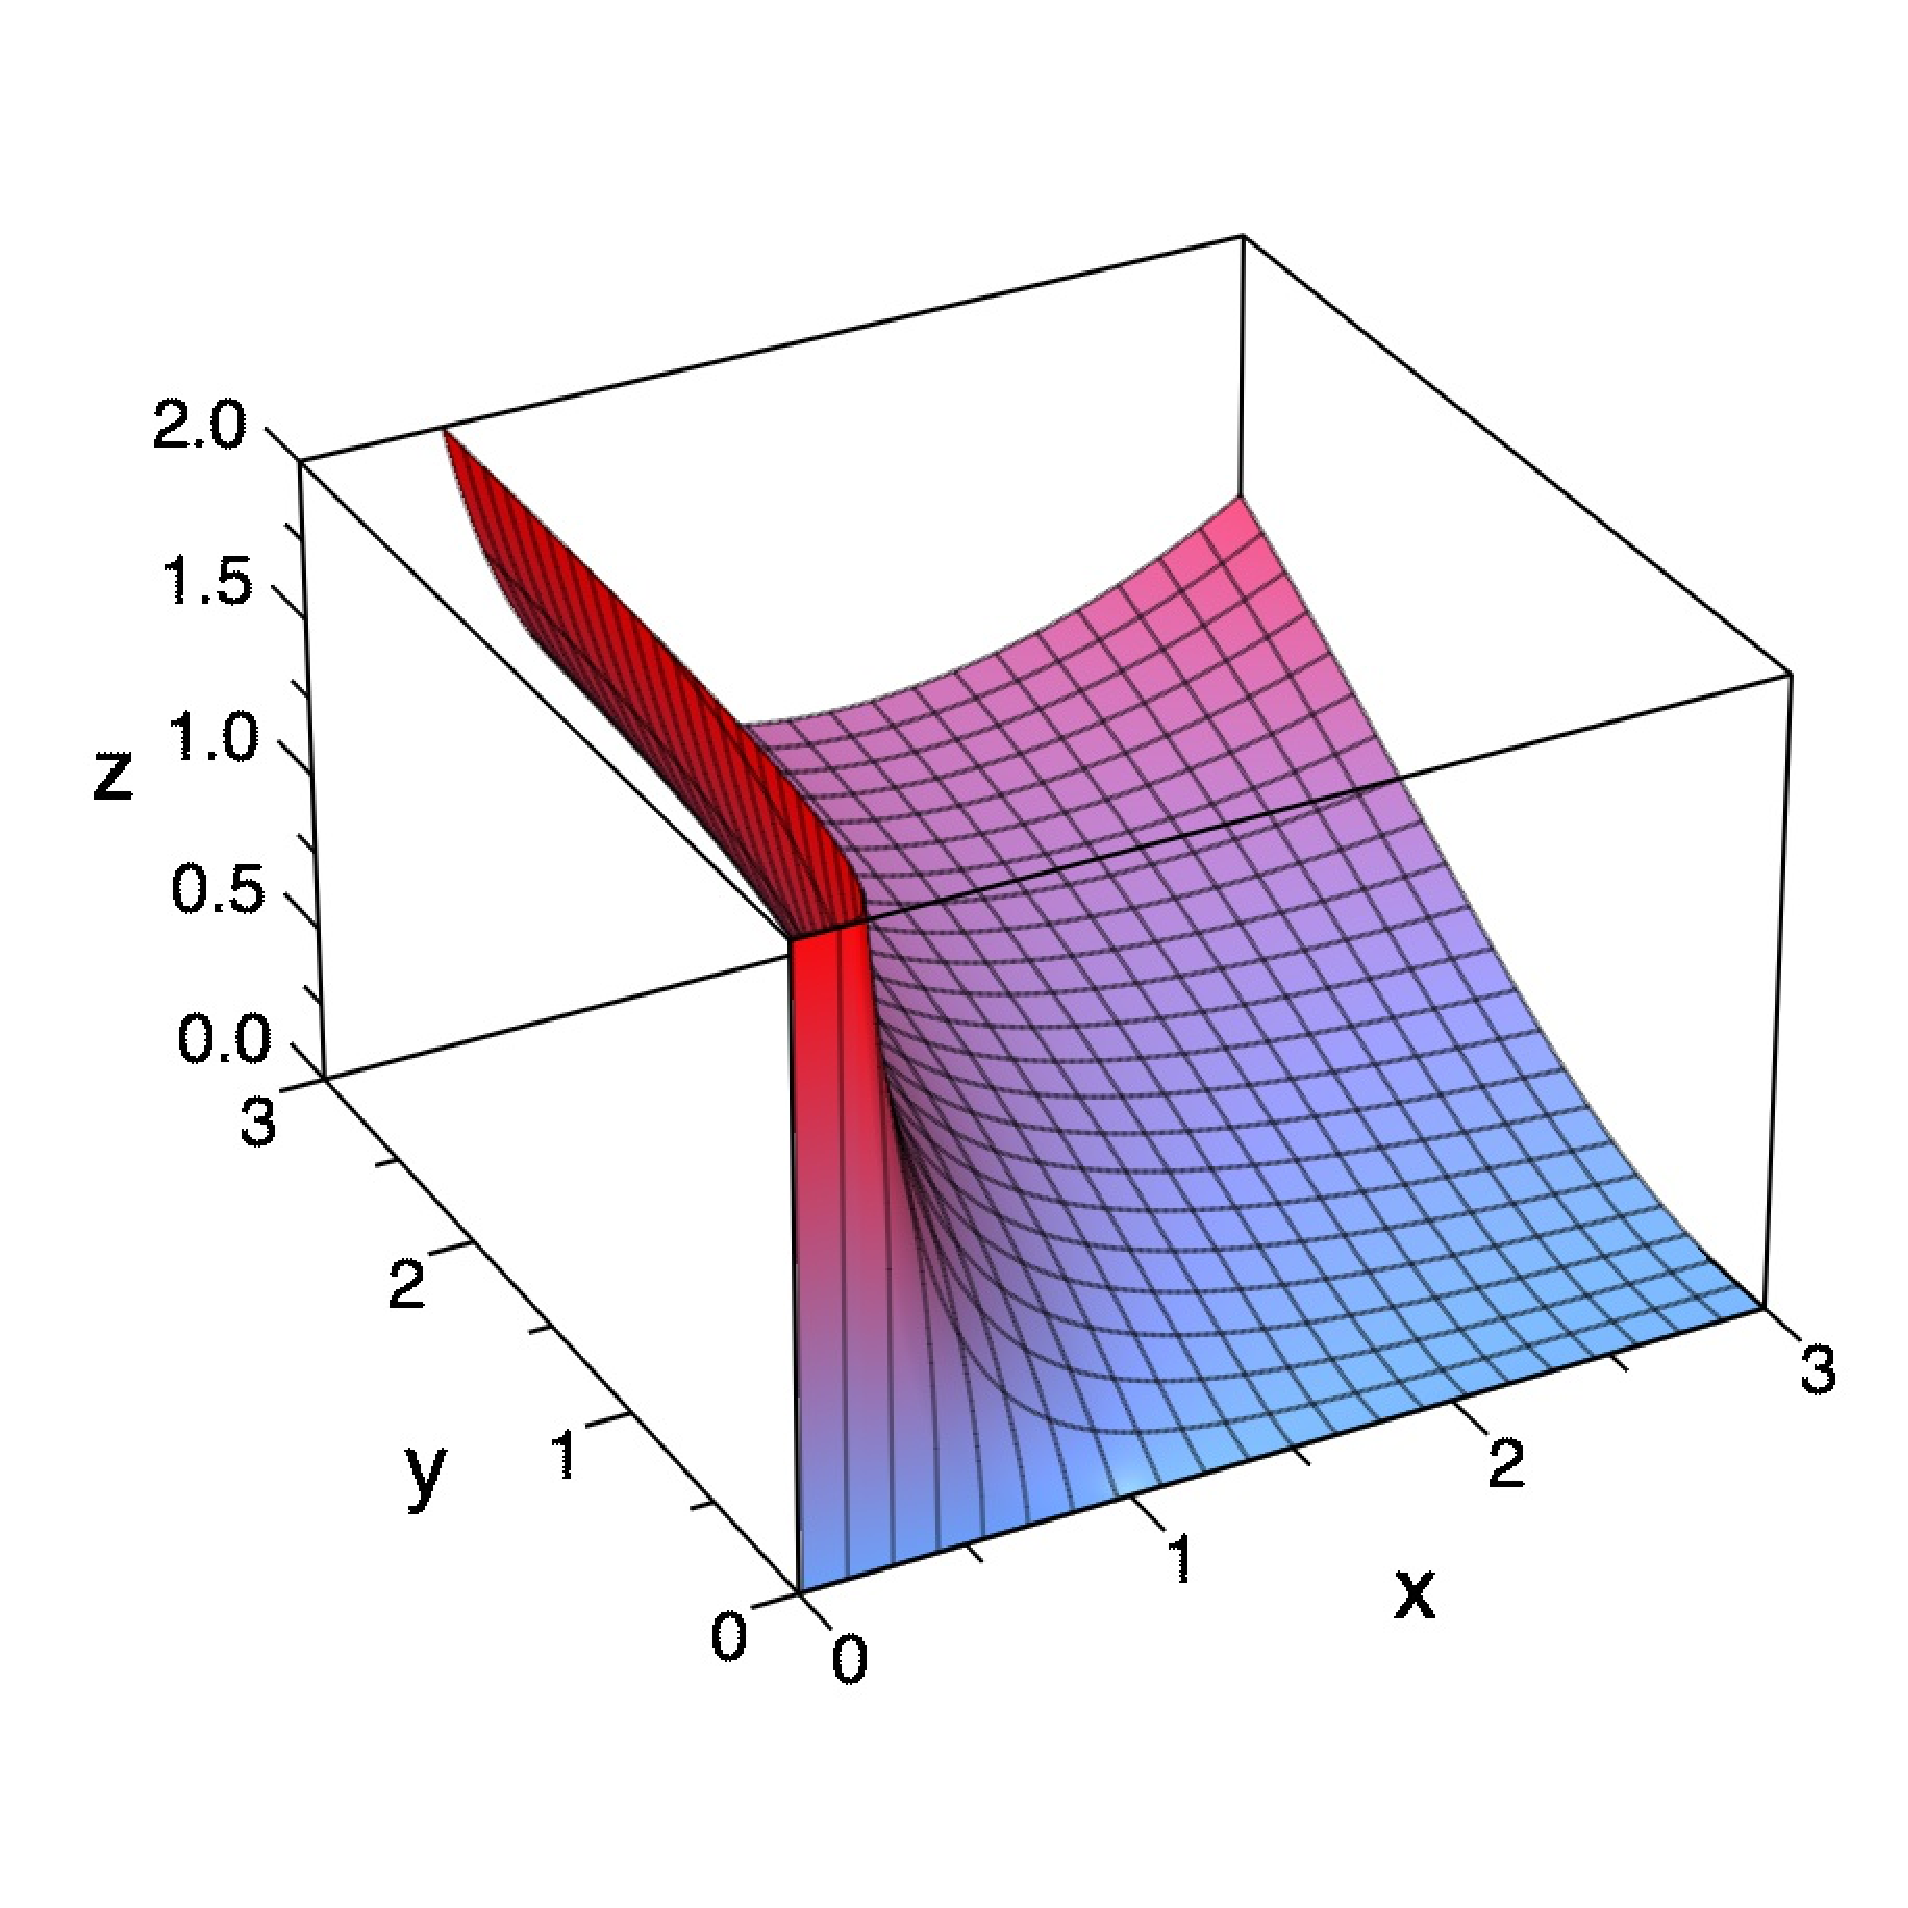
\includegraphics[width = 0.45\textwidth]{LowIncGamFunc.eps}
    }
\end{figure}

\begin{figure}[!ht]
    \centering
    \subfigure{
        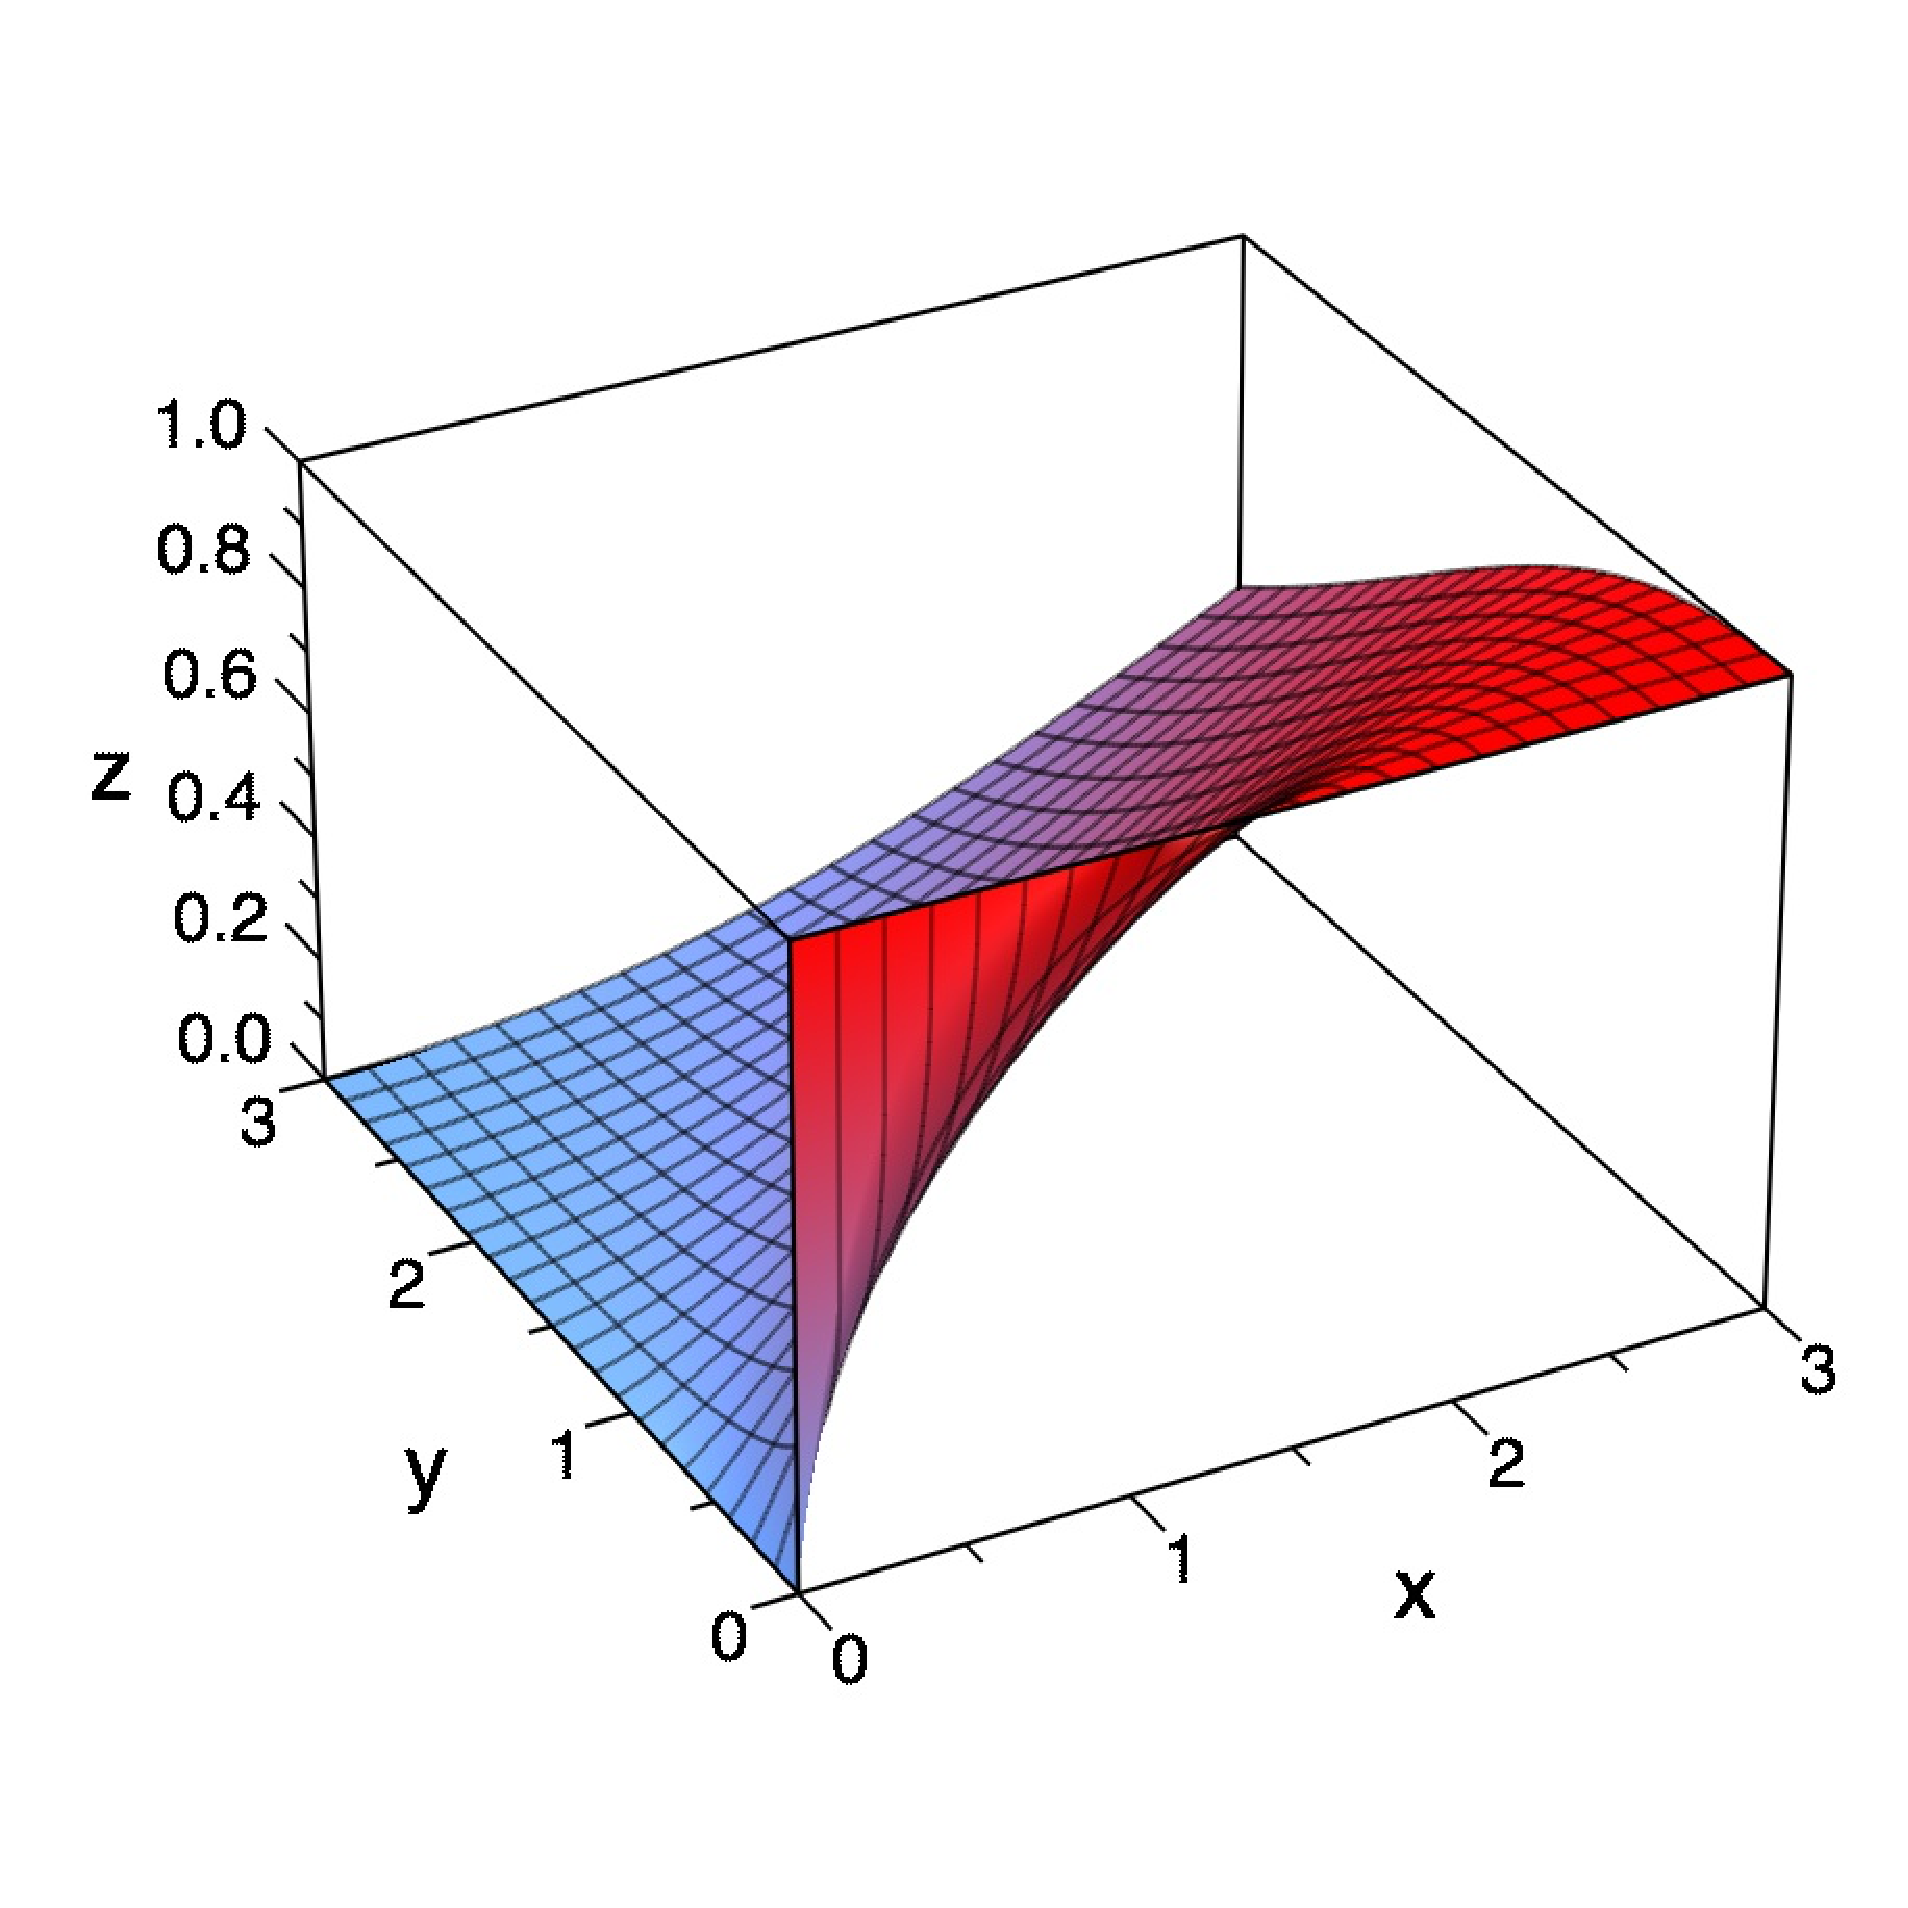
\includegraphics[width = 0.45\textwidth]{RegUppIncGamFunc.eps}
    }
    \subfigure{
        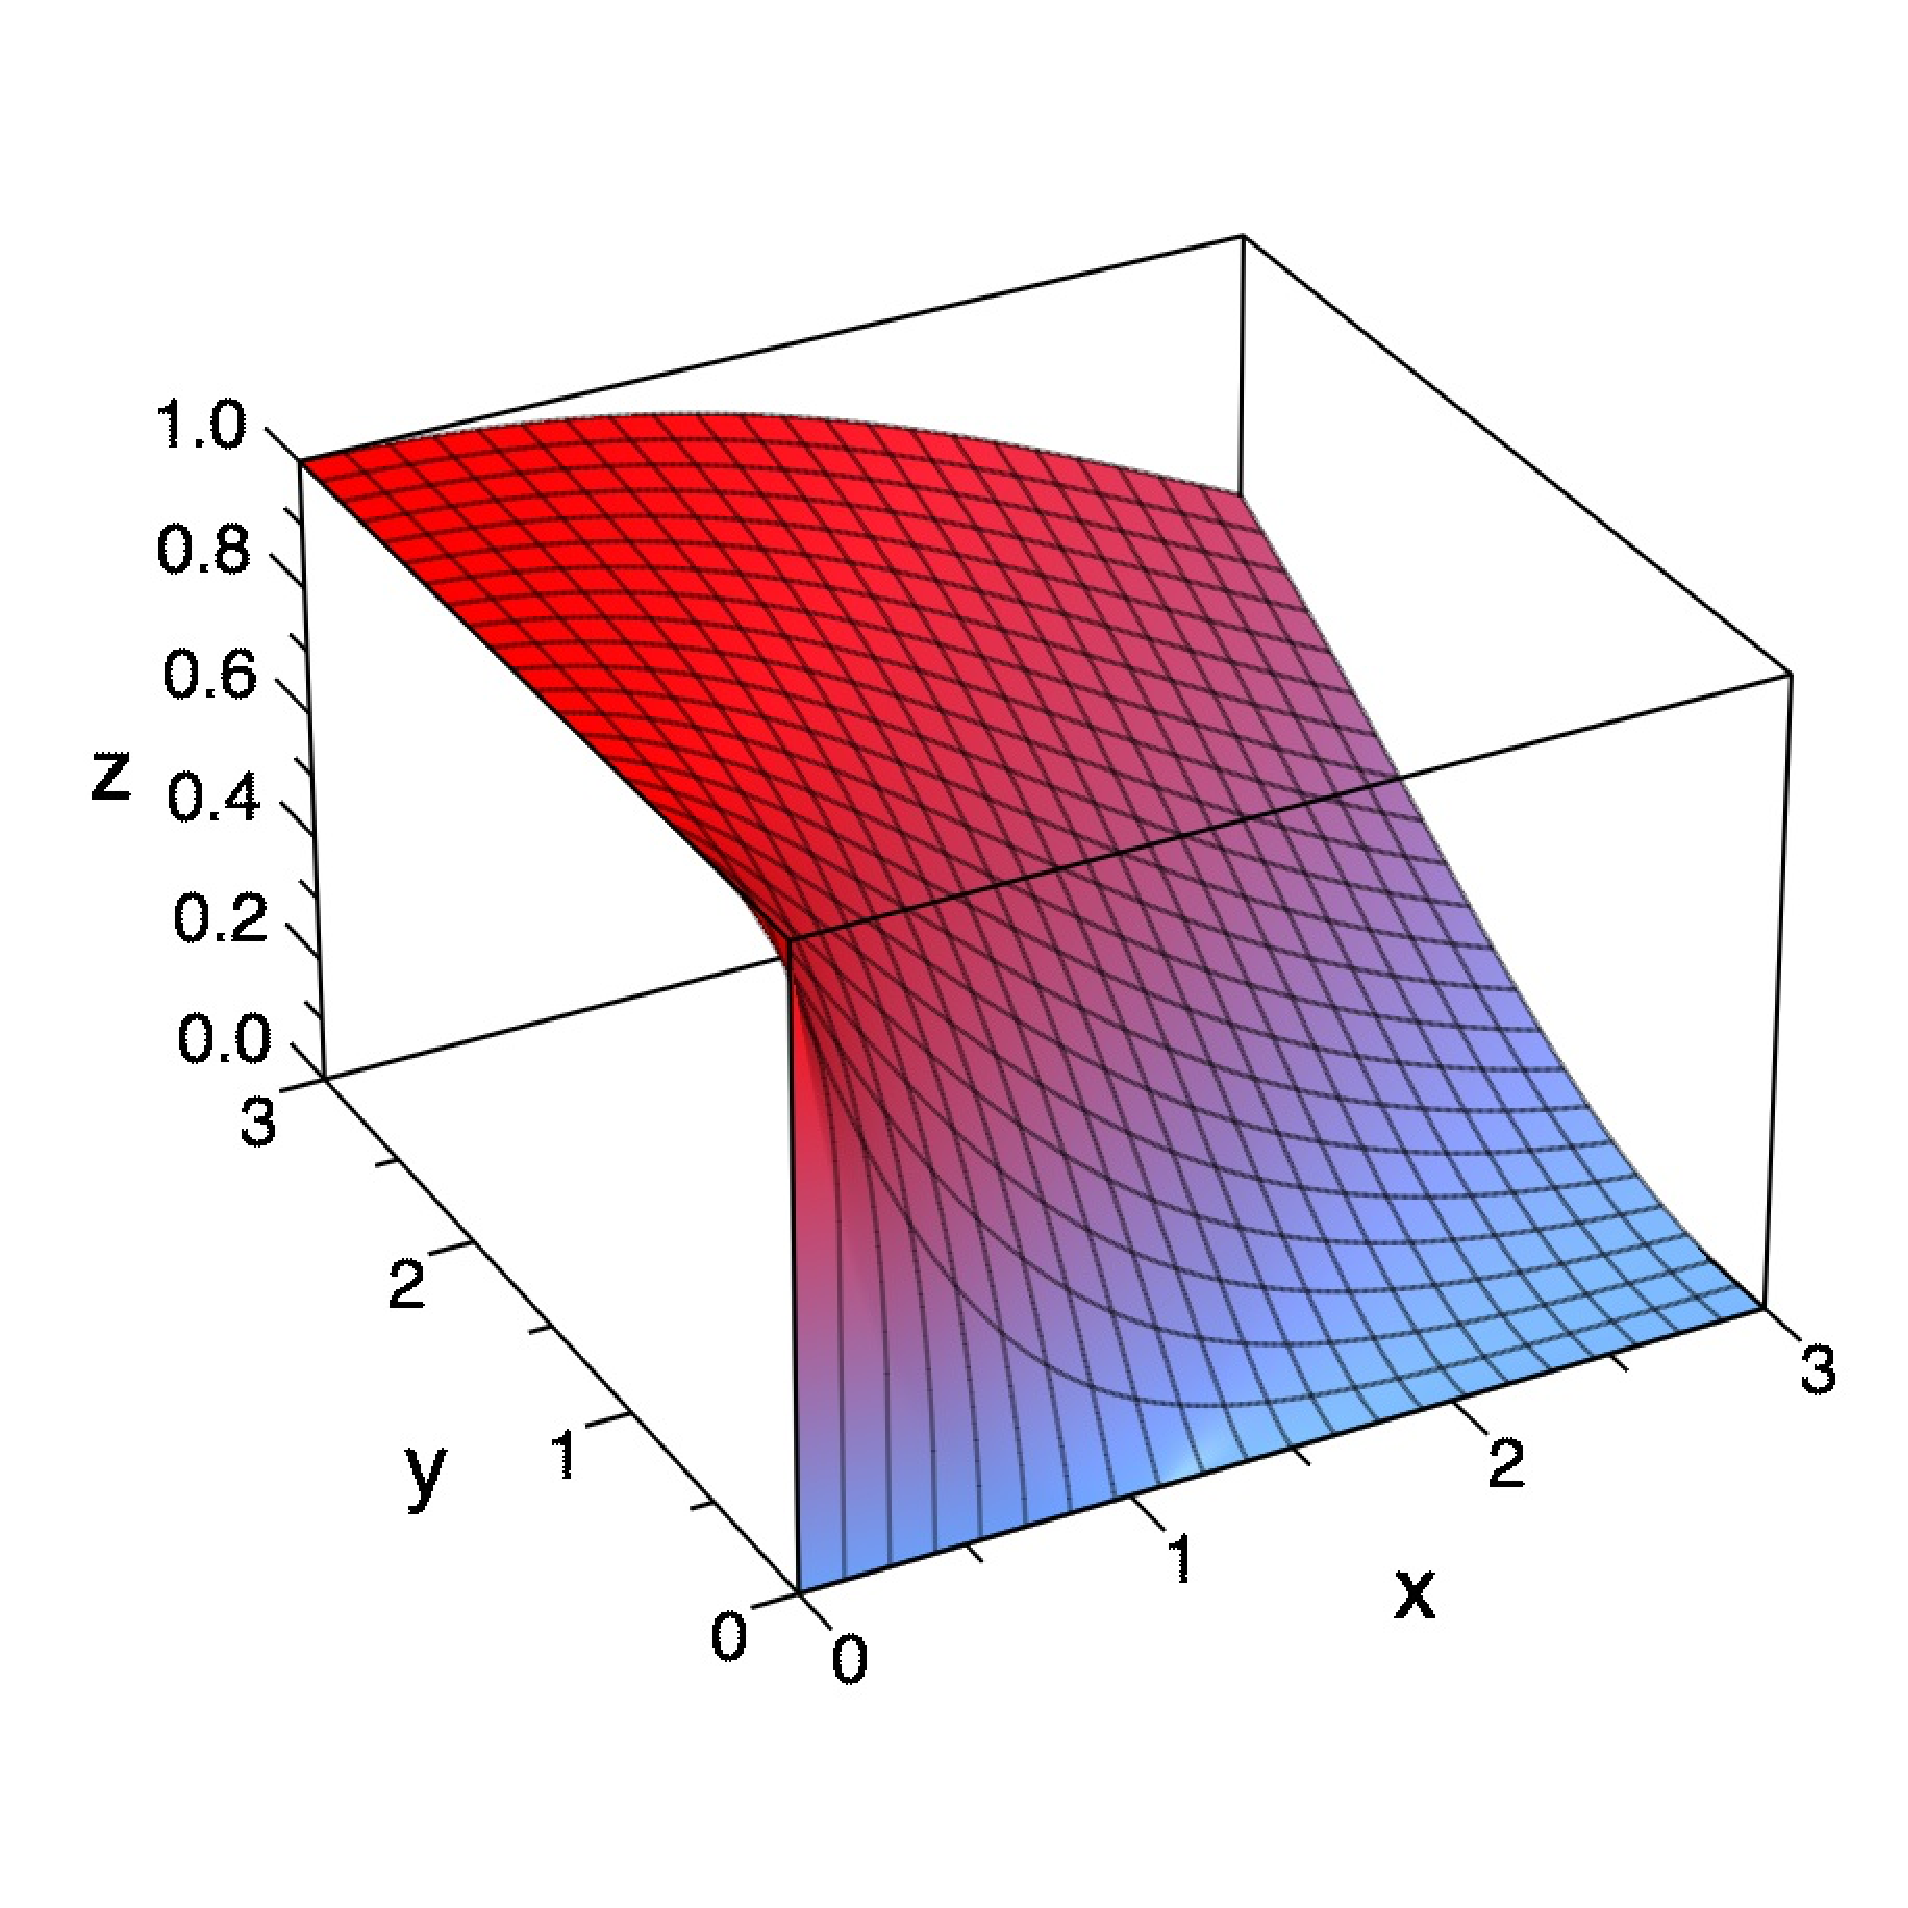
\includegraphics[width = 0.45\textwidth]{RegLowIncGamFunc.eps}
    }
    \caption{각종 불완전 감마함수의 그래프. 상부 불완전 감마함수 $z=\gamma(x,\,y)$ (왼쪽 위), 하부 불완전 감마함수 $z=\Gamma(x,\,y)$ (오른쪽 위), 정규화된 상부 불완전 감마함수 $z=Q(x,\,y)$ (왼쪽 아래), 정규화된 하부 불완전 감마함수 $z=P(x,\,y)$ (오른쪽 아래). (Rendered by MATLAB Symbolic Math Toolbox MuPAD.)}
\end{figure}

감마함수의 매우 중요한 성질 한가지를 소개한다. 이 정리는 감마함수의 존재 의의라 해도 과언이 아닐 정도로 감마함수의 본질을 관통하는 정리이다.

\begin{theorem}\label{thm:gammaFunc}
    임의의 $x>0$에 대해 $\Gamma(x+1)=x\Gamma(x)$이다.
\end{theorem}

\begin{proof}
    이는 $\Gamma(x+1)=\int_0^\infty t^xe^{-t}\,dt=[-t^xe^{-t}]_0^\infty+x\int_0^\infty t^{x-1}e^{-t}\,dt=x\Gamma(x)$로부터 자명하다.
\end{proof}

\begin{corollary}
    임의의 $n\in\mathbb{N}$에 대해 다음이 성립한다.
    \begin{enumerate}
        \item $\Gamma(n+1)=n!$.
        \item $\Gamma(n+1/2)=\sqrt{\pi}(2n-1)!!/2^n$. 단, 여기서 $(-1)!!=1$로 생각한다.
    \end{enumerate}
\end{corollary}

\begin{proof}
    i과 ii모두 정리 \ref{thm:gammaFunc}로부터 거의 자명하다. i의 경우 $\Gamma(1)=\int_0^\infty e^{-t}\,dt=[-e^{-t}]_0^\infty=1$에서 $\Gamma(n+1)=n\Gamma(n)=\cdots=n!\Gamma(1)=n!$임을 알 수 있고, ii의 경우에도 비슷하게 Gauss 적분으로부터 $\Gamma(1/2)=\int_0^\infty t^{-1/2}e^{-t}\,dt=2\int_0^\infty e^{-s^2}\,ds=\sqrt{\pi}$이므로 $\Gamma(n+1/2)=(n-1/2)\Gamma(n-1/2)=\cdots=(n-1/2)^{\underline{n}}\Gamma(1/2)=\sqrt{\pi}(2n-1)!!/2^n$임을 안다.
\end{proof}

따라서, 감마함수는 원래 음이 아닌 정수에 대해 정의되는 계승을 양의 실수로 일반화한 함수이다. 나아가, 비록 여기에서는 보이지는 않겠지만 Bohr-Mollerup 정리에 따르면 다음 함수 $f:\mathbb{R}^+\to\mathbb{R}^+$가 세 조건
\begin{enumerate}
    \item $f(1)=1$.
    \item 임의의 $x\in\mathbb{R}^+$에 대해 $f(x+1)=xf(x)$이다.
    \item 함수 $f$는 logarithmically convex하다. 즉, 함수 $\log f$가 볼록함수이다.
\end{enumerate}
을 만족하면 이는 감마함수이므로 이는 사실상 계승의 유일한 확장이라 해도 손색이 없다.

때로는 감마함수가 포함된 복잡한 극한을 계산해야 하는 경우도 있는데, 그 때에는 다음 결과가 굉장히 유용하다. 이 공식 역시 매우 유명한 공식이라 어디에선가 본 기억이 있을 수도 있다.

\begin{theorem}[Stirling's formula]
    임의의 $x>0$에 대해 다음이 성립한다.
    \begin{equation*}
        \bigg|\frac{\Gamma(x)}{\sqrt{2\pi/x}(x/e)^x}-1\bigg|\leq\sqrt{\frac{2}{\pi x}}
    \end{equation*}
\end{theorem}

\begin{proof}
    임의의 $x>0$를 고정하면 $\Gamma(x)=\int_0^\infty t^{x-1}e^{-t}\,dt=\int_{-1}^\infty [x(s+1)]^{x-1}e^{-x(s+1)}x\,ds=x^xe^{-x}\int_{-1}^\infty (s+1)^{x-1}e^{-sx}\,ds$이다. 여기서 두 번째 등호는 $s=t/x-1$의 변수변환으로부터 성립한다. 이제 $I=\int_{-1}^\infty (t+1)^{x-1}e^{-tx}\,dt$로 두면 $|I-\sqrt{2\pi/x}|\leq2/x$임을 보이는 것으로 증명은 충분하다. 이를 위해 함수 $f:(-1,\,\infty)\to\mathbb{R}$를
    \begin{equation*}
        f:t\mapsto\begin{dcases*}
            \sqrt{t-\log(t+1)}&$t\geq0$인 경우\\
            -\sqrt{t-\log(t+1)}&ow.
        \end{dcases*}
    \end{equation*}
    로 두면 이는 순증가하는 전단사함수이며 $[f(t)]^2=t-\log(t+1)$임을 쉽게 알 수 있다. 또한, 표기의 편의를 위해 $g=f^2$이라 하면 $g$는 $\mathcal{C}^\infty$급 함수가 되어 Taylor의 정리로부터 임의의 $t>-1$에 대해 $0$과 $t$사이의 적당한 $s_t\in\mathbb{R}$가 존재하여 $g(t)=g(0)+g'(0)t+g''(s_t)t^2/2=t^2/2(s_t+1)^2$이므로 $f(t)/t=1/\sqrt{2}(s_t+1)>0$이고, 곧 $|f(t)/t-2^{-1/2}|=|(s_t+1)^{-1}-1|/\sqrt{2}=|s_t|/\sqrt{2}(s_t+1)=|s_t|f(t)/t\leq|f(t)|$이다. 이로부터
    \begin{align*}
        I&=\int_{-1}^\infty(t+1)^{x-1}e^{-tx}\,dt\\
        &=\int_{-1}^\infty\exp(-x(t-\log(t+1)))\frac{1}{t+1}\,dt\\
        &=\int_{-\infty}^\infty e^{-xs^2}\frac{2s}{f^{-1}(s)}\,ds&\because s=f(t)
    \end{align*}
    에서
    \begin{align*}
        \bigg|I-\sqrt{2}\int_{-\infty}^\infty e^{-xs^2}\,ds\bigg|&=2\bigg|\int_{-\infty}^\infty e^{-xs^2}\bigg[\frac{s}{f^{-1}(s)}-\frac{1}{\sqrt{2}}\bigg]\,ds\bigg|\\
        &\leq2\int_{-\infty}^\infty e^{-xs^2}\bigg|\frac{f(f^{-1}(s))}{f^{-1}(s)}-\frac{1}{\sqrt{2}}\bigg|\,ds\\
        &\leq2\int_{-\infty}^\infty e^{-xs^2}|s|\,ds\\
        &=4\int_0^\infty se^{-xs^2}\,ds
    \end{align*}
    이고, 여기서 Gauss 적분으로부터 $\int_{-\infty}^\infty e^{-xs^2}\,ds=2\int_0^\infty e^{-xs^2}\,ds=2\int_0^\infty e^{-u^2}/\sqrt{x}\,du=\sqrt{\pi/x}$이고 $\int_0^\infty se^{-xs^2}\,ds=-[e^{-xs^2}]_0^\infty/2x=1/2x$이므로 이상을 종합하면 $|I-\sqrt{2\pi/x}|\leq2/x$임을 안다.
\end{proof}

\begin{figure}[!ht]
    \centering
    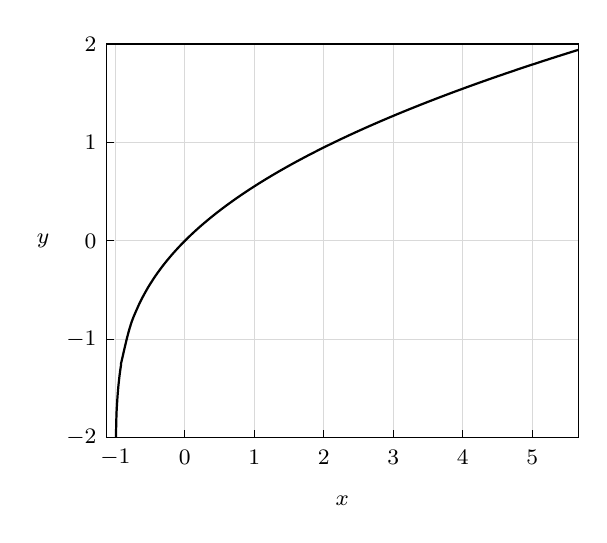
\begin{tikzpicture}
        \begin{scope}[every node/.append style = {font = \footnotesize}]
            \foreach \x in {-1, ..., 5} {
                \node at (6*\x/6.8,-2.75) {$\x$};
                \draw[style = thin, gray!30!white] (6*\x/6.8,-2.5) -- (6*\x/6.8,2.5);
                \draw (6*\x/6.8,-2.5) -- (6*\x/6.8,-2.4);
            }
            \foreach \y in {-2, ..., 2}
                \node[anchor = east] at (-1,5*\y/4) {$\y$};
            \foreach \y in {-1, 0, 1} {
                \draw[style = thin, gray!30!white] (-1,5*\y/4) -- (5,5*\y/4);
                \draw (-1,5*\y/4) -- (-0.9,5*\y/4);
            }
            \node at (2,-3.3) {$x$};
            \node at (-1.8,0) {$y$};
        \end{scope}
        \begin{scope}
        \draw[clip] (-1,-2.5) -- (5,-2.5) -- (5,2.5) -- (-1,2.5) -- cycle;
        \draw[style = thick] plot[smooth, tension = 0.7] coordinates{(-0.88,-2.77534) (-0.87,-2.26478) (-0.86,-2.05433) (-0.85,-1.91318) (-0.84,-1.80475) (-0.83,-1.7157) (-0.82,-1.63957) (-0.81,-1.57273) (-0.8,-1.51292) (-0.7,-1.10631) (-0.6,-0.84727) (-0.5,-0.649015) (-0.4,-0.485062) (-0.3,-0.343501) (-0.2,-0.217868) (-0.1,-0.10423) (0,0) (0.1,0.0966212) (0.2,0.186942) (0.3,0.271944) (0.4,0.352388) (0.5,0.428873) (0.6,0.501881) (0.7,0.571808) (0.8,0.638981) (0.9,0.703676) (1.,0.766126) (1.1,0.826532) (1.2,0.885066) (1.3,0.941879) (1.4,0.997103) (1.5,1.05085) (1.6,1.10324) (1.7,1.15434) (1.8,1.20425) (1.9,1.25304) (2.,1.30078) (2.1,1.34752) (2.2,1.39333) (2.3,1.43825) (2.4,1.48233) (2.5,1.52561) (2.6,1.56814) (2.7,1.60994) (2.8,1.65105) (2.9,1.6915) (3.,1.73133) (3.1,1.77055) (3.2,1.80919) (3.3,1.84728) (3.4,1.88484) (3.5,1.92188) (3.6,1.95843) (3.7,1.99451) (3.8,2.03013) (3.9,2.0653) (4.,2.10005) (4.1,2.13439) (4.2,2.16833) (4.3,2.20189) (4.4,2.23507) (4.5,2.26788) (4.6,2.30035) (4.7,2.33248) (4.8,2.36428) (4.9,2.39575) (5.,2.42692)};
        \end{scope}
    \end{tikzpicture}
    \caption{Stirling의 공식의 증명에서의 함수 $y=f(t)$의 그래프.}
\end{figure}

\begin{corollary}
    \begin{equation*}
        \lim_{x\to\infty}\frac{\Gamma(x)}{\sqrt{2\pi/x}(x/e)^x}=1
    \end{equation*}
\end{corollary}

\begin{proof}
    이는 Stirling의 공식으로부터 자명하다.
\end{proof}

\begin{figure}[!ht]
    \centering
    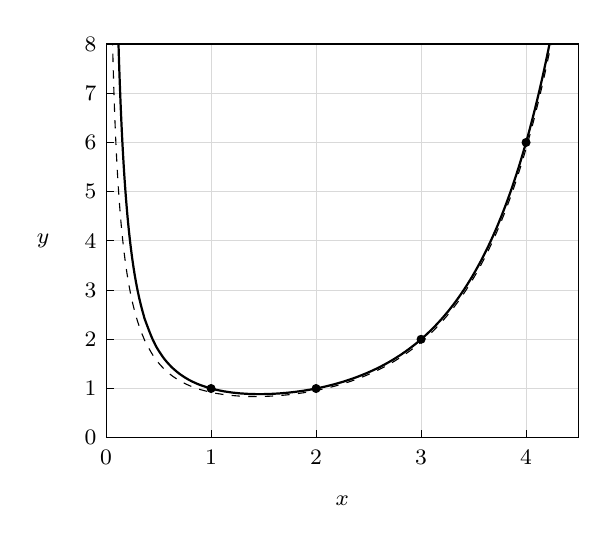
\begin{tikzpicture}
        \begin{scope}[every node/.append style = {font = \footnotesize}]
            \foreach \x in {0, ..., 4}
                \node at (6*\x/4.5,-0.25) {$\x$};
            \foreach \x in {1, ..., 4} {
                \draw[style = thin, gray!30!white] (6*\x/4.5,0) -- (6*\x/4.5,5);
                \draw (6*\x/4.5,0) -- (6*\x/4.5,0.1);
            }
            \foreach \y in {0, ..., 8} {
                \node[anchor = east] at (0,5*\y/8) {$\y$};
                \draw[style = thin, gray!30!white] (0,5*\y/8) -- (6,5*\y/8);
                \draw (0,5*\y/8) -- (0.1,5*\y/8);
            }
            \node at (3,-0.8) {$x$};
            \node at (-0.8,2.5) {$y$};
        \end{scope}
        \begin{scope}
        \draw[clip] (0,0) -- (6,0) -- (6,5) -- (0,5) -- cycle;
        \draw[style = thick] plot[smooth, tension = 0.7] coordinates{(0.14,5.65092) (0.16,4.91453) (0.18,4.34331) (0.2,3.88767) (0.22,3.51604) (0.24,3.20739) (0.26,2.94715) (0.28,2.72493) (0.3,2.5331) (0.32,2.36594) (0.34,2.21908) (0.36,2.08913) (0.38,1.97339) (0.4,1.86973) (0.42,1.77641) (0.44,1.692) (0.46,1.61535) (0.48,1.54546) (0.5,1.48152) (0.6,1.23009) (0.7,1.0563) (0.8,0.930745) (0.9,0.837166) (1,0.765885) (1.1,0.710802) (1.2,0.667893) (1.3,0.634414) (1.4,0.60844) (1.5,0.588589) (1.6,0.573855) (1.7,0.563498) (1.8,0.55697) (1.9,0.553866) (2,0.553892) (2.1,0.55684) (2.2,0.562573) (2.3,0.571008) (2.4,0.582115) (2.5,0.595904) (2.6,0.612425) (2.7,0.631768) (2.8,0.654054) (2.9,0.679442) (3,0.708127) (3.1,0.740341) (3.2,0.776356) (3.3,0.816486) (3.4,0.861091) (3.5,0.910583) (3.6,0.965429) (3.7,1.02616) (3.8,1.09336) (3.9,1.16772) (4,1.25) (4.1,1.34105) (4.2,1.44184) (4.3,1.55346) (4.4,1.67715) (4.5,1.81429) (4.6,1.96645) (4.7,2.1354) (4.8,2.32314) (4.9,2.53194) (5,2.76437) (5.1,3.02332) (5.2,3.31208) (5.3,3.63439) (5.4,3.99449) (5.5,4.39718) (5.6,4.84793) (5.7,5.35298)};
        \draw[style = dashed] plot[smooth, tension = 0.7] coordinates{(0.08,5.08775) (0.1,4.37015) (0.12,3.84277) (0.14,3.43557) (0.16,3.11004) (0.18,2.84294) (0.2,2.61935) (0.22,2.42915) (0.24,2.26522) (0.26,2.12237) (0.28,1.99675) (0.3,1.8854) (0.32,1.78601) (0.34,1.69677) (0.36,1.61621) (0.38,1.54314) (0.4,1.47658) (0.42,1.41573) (0.44,1.3599) (0.46,1.30851) (0.48,1.26108) (0.5,1.21718) (0.6,1.03963) (0.7,0.911946) (0.8,0.816974) (0.9,0.744645) (1,0.688675) (1.1,0.644948) (1.2,0.610663) (1.3,0.583862) (1.4,0.563138) (1.5,0.547468) (1.6,0.536097) (1.7,0.528463) (1.8,0.524151) (1.9,0.522852) (2,0.524348) (2.1,0.528485) (2.2,0.535169) (2.3,0.54435) (2.4,0.556025) (2.5,0.570223) (2.6,0.587011) (2.7,0.606487) (2.8,0.628785) (2.9,0.654069) (3,0.682538) (3.1,0.714426) (3.2,0.750006) (3.3,0.789591) (3.4,0.83354) (3.5,0.88226) (3.6,0.936214) (3.7,0.995924) (3.8,1.06198) (3.9,1.13505) (4,1.21588) (4.1,1.30532) (4.2,1.40432) (4.3,1.51396) (4.4,1.63545) (4.5,1.77016) (4.6,1.91964) (4.7,2.08563) (4.8,2.27011) (4.9,2.47531) (5,2.70375) (5.1,2.95831) (5.2,3.24221) (5.3,3.55915) (5.4,3.9133) (5.5,4.3094) (5.6,4.75287) (5.7,5.24983) (5.8,5.80728) (5.9,6.43319) (6,7.13666)};
        \end{scope}
        \draw[fill = black] (6/4.5,5/8) circle[radius = 0.05];
        \draw[fill = black] (12/4.5,5/8) circle[radius = 0.05];
        \draw[fill = black] (18/4.5,10/8) circle[radius = 0.05];
        \draw[fill = black] (24/4.5,30/8) circle[radius = 0.05];
    \end{tikzpicture}
    \caption{감마함수(실선)의 Stirling 근사(점선).}
\end{figure}

이로부터 충분히 큰 $x>0$에 대해 $\Gamma(x)$의 값을 $\sqrt{2\pi/x}(x/e)^x$로 근사할 수 있고, 이를 흔히 감마함수의 Stirling 근사라 부른다.\footnote{
    다만, Stirling의 공식은 어디까지나 $x$가 충분히 크면 참값 $\Gamma(x)$와 근삿값 $\sqrt{2\pi/x}(x/e)^x$의 비가 $1$에 가까워짐을 의미하는 것이지, 오차 $\sqrt{2\pi/x}(x/e)^x-\Gamma(x)$가 $0$에 가까워짐을 뜻하는 것은 아님에 주의해야 한다. 실제로 참값과 근삿값의 비가 $1$로 가까워지는 속도(대략 $x^{-1/2}$)보다 참값이 증가하는 속도($x^x$보다 빠름)가 압도적으로 빨라 오차는 $x$가 커짐에 따라 계속 커진다.
}

감마함수의 근사에 대해서는 이정도로 마무리하고, 이제 감마함수의 무한곱 표현에 대해 알아보자. 앞서 감마함수는 적분으로 정의되었는데, 때로는 이러한 적분의 형태가 감마함수의 성질을 밝히는데 불편한 경우가 있다. 이때 감마함수의 무한곱 형태가 도움이 될 수 있다. 이를 위해선, 우선 감마함수와 밀접히 다음 상수가 필요하다.

\begin{definition}
    수열 $\{H_n\}$을 $H_n=\sum_{k=1}^n1/k$라 하자. 이때 $\{H_n-\log n\}$의 극한값을 \textbf{Euler-Mascheroni 상수(- constant)} 혹은 간단히 \textbf{Euler 상수(- constant)}라 하고 $\gamma$로 쓴다.
\end{definition}

\begin{proposition}\label{prop:eulerConstant}
    수열 $\{H_n\}$을 $H_n=\sum_{k=1}^n1/k$라 하면 $\{H_n-\log n\}$는 수렴한다. 따라서 Euler 상수는 well-define된다.
\end{proposition}

\begin{proof}
    표기의 편의를 위해 수열 $\{a_n\}$을 $a_n=H_n-\log n$으로 두면 임의의 $n\in\mathbb{N}$에 대해 $a_{n+1}-a_n=1/(n+1)-\log(n+1)+\log n=1/(n+1)+\log(1-1/(n+1))$인데, $(-\infty,\,1)$에서 정의된 함수 $x\mapsto x+\log(1-x)$가 양이 아님을 쉽게 알 수 있으므로 곧 $\{a_n\}$은 단조감소한다. 한편, 임의의 $n\in\mathbb{N}$에 대해 $\log(n+1)=\int_1^{n+1}1/x\,dx\leq H_n$이므로 $a_n\geq\log(n+1)-\log n=\log(1+1/n)\geq0$이 되어 $\{a_n\}$은 $0$에 의해 아래로 유계이다. 그렇다면 MSP로부터 $\{a_n\}$이 수렴하고, 곧 증명이 끝난다.
\end{proof}

\begin{figure}[!ht]
    \centering
    \subfigure{
        \begin{tikzpicture}
            \draw[->] (-0.2,0) -- (5,0) node[below] {$n$};
            \draw[->] (0,-0.2) -- (0,2.5);
            \begin{scope}
                \clip (-0.2,-0.2) -- (-0.2,2.5) -- (4.9,2.5) -- (4.9,-0.2) -- cycle;
                \draw (0.909091,1.5) -- (1.81818,1.21028) -- (2.72727,1.10208) -- (3.63636,1.04556) -- (4.54545,1.01084) -- (5.45455,0.987361);
            \end{scope}
            \draw[fill = black] (0.909091,1.5) circle[radius = 0.05];
            \draw[fill = black] (1.81818,1.21028) circle[radius = 0.05];
            \draw[fill = black] (2.72727,1.10208) circle[radius = 0.05];
            \draw[fill = black] (3.63636,1.04556) circle[radius = 0.05];
            \draw[fill = black] (4.54545,1.01084) circle[radius = 0.05];
            \begin{scope}[style = dashed]
                \draw (0.909091,0) -- (0.909091,1.5);
                \draw (1.81818,0) -- (1.81818,1.21028);
                \draw (2.72727,0) -- (2.72727,1.10208);
                \draw (3.63636,0) -- (3.63636,1.04556);
                \draw (4.54545,0) -- (4.54545,1.01084);
                \draw (0,0.865823) -- (4.9,0.865823);
            \end{scope}
            \begin{scope}[every node/.append style = {font = \footnotesize}]
                \node at (0.909091,-0.2) {$1$};
                \node at (1.81818,-0.2) {$2$};
                \node at (2.72727,-0.2) {$3$};
                \node at (3.63636,-0.2) {$4$};
                \node at (4.54545,-0.2) {$5$};
                \node at (-0.2,0.865823) {$\gamma$};
            \end{scope}
        \end{tikzpicture}
    }
    \qquad
    \subfigure{
        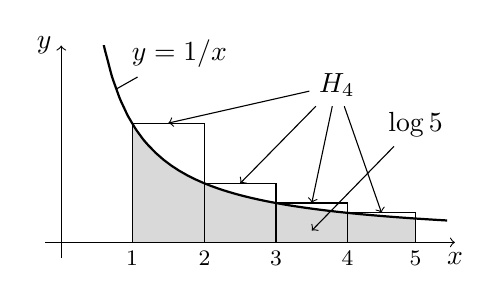
\begin{tikzpicture}
            \fill[fill = gray!30!white] (0.9,0) -- plot[smooth, tension = 1] coordinates{(0.9,1.51515) (1,1.36364) (1.1,1.23967) (1.2,1.13636) (1.3,1.04895) (1.4,0.974026) (1.5,0.909091) (1.6,0.852273) (1.7,0.802139) (1.8,0.757576) (1.9,0.717703) (2,0.681818) (2.1,0.649351) (2.2,0.619835) (2.3,0.592885) (2.4,0.568182) (2.5,0.545455) (2.6,0.524476) (2.7,0.505051) (2.8,0.487013) (2.9,0.470219) (3,0.454545) (3.1,0.439883) (3.2,0.426136) (3.3,0.413223) (3.4,0.40107) (3.5,0.38961) (3.6,0.378788) (3.7,0.36855) (3.8,0.358852) (3.9,0.34965) (4,0.340909) (4.1,0.332594) (4.2,0.324675) (4.3,0.317125) (4.4,0.309917) (4.5,0.30303)} -- (4.5,0) -- cycle;
            \draw[->] (-0.2,0) -- (5,0) node[below] {$x$};
            \draw[->] (0,-0.2) -- (0,2.5) node[left] {$y$};
            \begin{scope}
                \clip (-0.2,-0.2) -- (-0.2,2.5) -- (4.9,2.5) -- (4.9,-0.2) -- cycle;
                \draw[style = thick] plot[smooth, tension = 1] coordinates{(0.1,13.6364) (0.2,6.81818) (0.3,4.54545) (0.4,3.40909) (0.5,2.72727) (0.6,2.27273) (0.7,1.94805) (0.8,1.70455) (0.9,1.51515) (1,1.36364) (1.1,1.23967) (1.2,1.13636) (1.3,1.04895) (1.4,0.974026) (1.5,0.909091) (1.6,0.852273) (1.7,0.802139) (1.8,0.757576) (1.9,0.717703) (2,0.681818) (2.1,0.649351) (2.2,0.619835) (2.3,0.592885) (2.4,0.568182) (2.5,0.545455) (2.6,0.524476) (2.7,0.505051) (2.8,0.487013) (2.9,0.470219) (3,0.454545) (3.1,0.439883) (3.2,0.426136) (3.3,0.413223) (3.4,0.40107) (3.5,0.38961) (3.6,0.378788) (3.7,0.36855) (3.8,0.358852) (3.9,0.34965) (4,0.340909) (4.1,0.332594) (4.2,0.324675) (4.3,0.317125) (4.4,0.309917) (4.5,0.30303) (4.6,0.296443) (4.7,0.290135) (4.8,0.284091) (4.9,0.278293)};
            \end{scope}
            \begin{scope}
                \draw (0.9,0) -- (0.9,1.51515) -- (10/5.5,1.51515) -- (10/5.5,0);
                \draw (10/5.5,0.75) -- (15/5.5,0.75) -- (15/5.5,0);
                \draw (15/5.5,0.5) -- (20/5.5,0.5) -- (20/5.5,0);
                \draw (20/5.5,1.5/4) -- (4.5,1.5/4) -- (4.5,0);
            \end{scope}
            \begin{scope}[every node/.append style = {font = \footnotesize}]
                \node at (0.9,-0.2) {$1$};
                \node at (10/5.5,-0.2) {$2$};
                \node at (15/5.5,-0.2) {$3$};
                \node at (20/5.5,-0.2) {$4$};
                \node at (4.5,-0.2) {$5$};
            \end{scope}
            \node (a) at (3.5,2) {$H_4$};
            \node (b) at (4.5,1.5) {$\log 5$};
            \node (c) at (1.5,2.4) {$y=1/x$};
            \draw[->] (a) -- (1.359,1.51515);
            \draw[->] (a) -- (25/11,0.75);
            \draw[->] (a) -- (35/11,0.5);
            \draw[->] (a) -- (4.068,1.5/4);
            \draw[->] (b) -- (35/11,0.15);
            \draw (c) -- (0.7,1.94805);
        \end{tikzpicture}
    }
    \caption{명제 \ref{prop:eulerConstant}에서의 수열 $\{H_n-\log n\}$의 그래프(왼쪽)와 이의 증명에서의 부등식 $\log(n+1)\leq H_n$의 $n=4$인 경우(오른쪽).}
\end{figure}

약 $0.577216$으로 알려진 $\gamma$는 아직까지 유리수인지 무리수인지조차 밝혀지지 않았을 정도로 많은 성질들이 베일에 가려져 있는 신비한 상수 중 하나이다. 이 책에서는 감마함수의 무한곱 표현을 위해서만 사용될 것이므로 이에 대해 더 깊이 다루지는 않겠다. 이제 Stirling의 공식의 도움을 받아 감마함수를 무한곱의 형태로 나타낼 수 있다.

\begin{lemma}
    임의의 $\alpha>0$에 대해 $\lim_{x\to\infty}\Gamma(x+\alpha)/x^\alpha\Gamma(x)=1$이다.
\end{lemma}

\begin{proof}
    Stirling의 공식으로부터
    \begin{align*}
        \lim_{x\to\infty}\frac{\Gamma(x+\alpha)}{x^\alpha\Gamma(x)}&=\lim_{x\to\infty}\sqrt{\frac{2\pi}{x+\alpha}}\bigg(\frac{x+\alpha}{e}\bigg)^{x+\alpha}\bigg/x^\alpha\sqrt{\frac{2\pi}{x}}\bigg(\frac{x}{e}\bigg)^x\\
        &=e^{-\alpha}\lim_{x\to\infty}\bigg(1+\frac{\alpha}{x}\bigg)^{x+\alpha-1/2}\\
        &=1
    \end{align*}
    이므로 보조정리는 자명하다.
\end{proof}

\begin{theorem}[Weierstrass]
    임의의 $x>0$에 대해서 다음의 성립한다.
    \begin{equation*}
        \Gamma(x)=\frac{e^{-\gamma x}}{x}\prod_{k=1}^\infty\bigg(1+\frac{x}{k}\bigg)^{-1}e^{x/k}
    \end{equation*}
\end{theorem}

\begin{proof}
    임의의 $x>0$를 고정하고 수열 $\{H_n\}$을 $H_n=\sum_{k=1}^n1/k$라 하자. 이제 임의의 $n\in\mathbb{N}$에 대해 $P_n:=x\prod_{k=1}^{n-1}(1+x/k)e^{-x/k}=x^{\overline{n}}e^{(1/n-H_n)x}/\Gamma(n)$으로 두면 $\Gamma(x)=\Gamma(x+n)/x^{\overline{n}}=\Gamma(x+n)/P_n\Gamma(n)e^{(H_n-1/n)x}=[\Gamma(x+n)/n^x\Gamma(n)]e^{x/n}/P_ne^{(H_n-\log n)x}$인데 보조정리와 Euler 상수의 정의로부터 $n\to\infty$이면 $\Gamma(x+n)/n^x\Gamma(n)\to1$이고 $H_n-\log n\to\gamma$이므로 $P_n\to e^{-\gamma x}/\Gamma(x)$가 되고, 증명은 이로써 충분하다.
\end{proof}

경우에 따라서는 이와 같은 무한곱의 형태를 감마함수의 정의로 두는 경우도 있으며 이는 Weierstrass의 방식이라 불린다. 이러한 무한곱의 형태는 잠시 후, 프사이함수와 polygamma 함수의 성질의 증명에 요긴하게 쓰일 것이다.

마지막으로 감마함수가 $\mathcal{C}^\infty$급임을 보이는 것으로 끝으로 감마함수에 대한 내용은 마무리하도록 하자.

\begin{theorem}
    감마함수는 $\mathcal{C}^\infty$급 함수이며 임의의 $n\in\mathbb{N}$에 대해 $\Gamma^{(n)}(x)=\int_0^\infty (\log t)^nt^{x-1}e^{-t}\,dt$이다.
\end{theorem}

\begin{proof}
    임의의 $x_0>0$와 임의의 $n\in\mathbb{N}_0$을 고정하고 $x_0\in(a,\,b)=:I$인 적당한 $a,\,b>0$를 택하여 함수 $f:\mathbb{R}^+\times I\to\mathbb{R}$를 $f:(t,\,x)\mapsto (\log t)^nt^{x-1}e^{-t}$로 정의하자. 그렇다면 $f$는 Leibniz의 법칙의 조건 i, ii를 만족함이 분명하고 임의의 $(t,\,x)\in\mathbb{R}^+\times I$에 대해
    \begin{align*}
        \bigg|\frac{\partial}{\partial x}f(t,\,x)\bigg|&=|\log t|^{n+1}t^{x-1}e^{-t}\\
        &\leq t^{x+n}e^{-t}\ind_{[1,\,\infty)}(t)+|\log t|^{n+1}t^{x-1}\ind_{(0,\,1)}(t)\\
        &\leq t^{b+n}e^{-t}\ind_{[1,\,\infty)}(t)+|\log t|^{n+1}t^{a-1}\ind_{(0,\,1)}(t)\\
        &\leq t^{b+n}e^{-t}+(-\log t)^{n+1}t^{a-1}\ind_{(0,\,1)}(t)
    \end{align*}
    이다. 여기서 첫 번째 부등호는 임의의 $t\in\mathbb{R}$에 대해 $\log t\leq t$이므로 성립한다. 한편, $\int_0^\infty t^{b+n}e^{-t}\,dt=\Gamma(n+b+1)$이고
    \begin{align*}
        \int_0^1(-\log t)^{n+1}t^{a-1}\,dt&=\bigg[(-\log t)^{n+1}\frac{t^a}{a}\bigg]_0^1+\frac{n+1}{a}\int_0^1(-\log t)^nt^{a-1}\,dt\\
        &=\cdots\\
        &=(n+1)!\bigg[\frac{t^a}{a^{n+2}}\bigg]_0^1\\
        &=\frac{(n+1)!}{a^{n+2}}
    \end{align*}
    에서 함수 $t\mapsto t^{b+n}e^{-t}+(-\log t)^{n+1}t^{a-1}\ind_{(0,\,1)}(t)$가 적분가능하여 $f$가 Leibniz의 법칙의 조건 iii도 만족시킴을 알고, 곧 이로부터 함수 $x\mapsto\int_0^\infty (\log t)^nt^{x-1}e^{-t}\,dt$는 $x_0$에서 미분가능하며 그 미분계수는 $\int_0^\infty (\log t)^{n+1}t^{x-1}e^{-t}\,dt$로 주어진다. 증명은 이로써 충분하다.
\end{proof}

\begin{figure}[!ht]
    \centering
    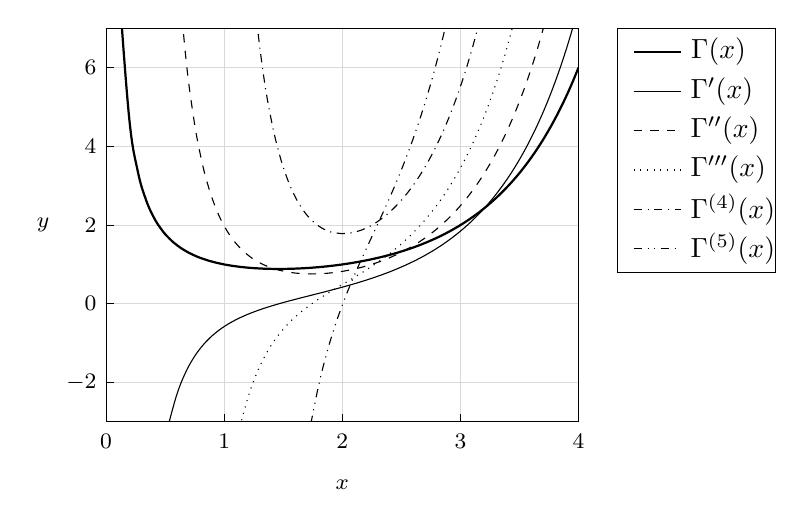
\begin{tikzpicture}
        \begin{scope}[every node/.append style = {font = \footnotesize}]
            \foreach \x in {0, ..., 4}
                \node at (6*\x/4,-1.75) {$\x$};
            \foreach \x in {1, 2, 3} {
                \draw[style = thin, gray!30!white] (6*\x/4,-1.5) -- (6*\x/4,3.5);
                \draw (6*\x/4,-1.5) -- (6*\x/4,-1.4);
            }
            \foreach \y in {-2, 0, ..., 6} {
                \node[anchor = east] at (0,\y/2) {$\y$};    \draw[style = thin, gray!30!white] (0,\y/2) -- (6,\y/2);
                \draw (0,\y/2) -- (0.1,\y/2);
            }
            \node at (3,-2.3) {$x$};
            \node at (-0.8,1) {$y$};
        \end{scope}
        \begin{scope}
        \draw[clip] (0,-1.5) -- (6,-1.5) -- (6,3.5) -- (0,3.5) -- cycle;
        \draw[style = thick] plot[smooth, tension = 0.7] coordinates{(0.2,3.52029) (0.3,2.29542) (0.4,1.69335) (0.5,1.33947) (0.6,1.10908) (0.7,0.948872) (0.8,0.832277) (0.9,0.744596) (1,0.677059) (1.1,0.624121) (1.2,0.582115) (1.3,0.548527) (1.4,0.521583) (1.5,0.5) (1.6,0.482832) (1.7,0.469372) (1.8,0.459084) (1.9,0.451561) (2,0.44649) (2.1,0.443632) (2.2,0.442807) (2.3,0.443881) (2.4,0.446758) (2.5,0.451373) (2.6,0.457689) (2.7,0.465692) (2.8,0.47539) (2.9,0.486811) (3,0.5) (3.1,0.515021) (3.2,0.531955) (3.3,0.550901) (3.4,0.571977) (3.5,0.59532) (3.6,0.621085) (3.7,0.64945) (3.8,0.680618) (3.9,0.714812) (4,0.752288) (4.1,0.793327) (4.2,0.838245) (4.3,0.887395) (4.4,0.941168) (4.5,1.) (4.6,1.06438) (4.7,1.13484) (4.8,1.21198) (4.9,1.29648) (5,1.38908) (5.1,1.4906) (5.2,1.60198) (5.3,1.72423) (5.4,1.85851) (5.5,2.0061) (5.6,2.16843) (5.7,2.34709) (5.8,2.54387) (5.9,2.76076) (6,3)};
        \draw plot[smooth, tension = 0.7] coordinates{(0.8,-1.50459) (0.9,-1.14714) (1,-0.892522) (1.1,-0.704618) (1.2,-0.561746) (1.3,-0.45026) (1.4,-0.361229) (1.5,-0.288608) (1.6,-0.228184) (1.7,-0.176946) (1.8,-0.132694) (1.9,-0.0937804) (2,-0.0589517) (2.1,-0.0272321) (2.2,0.0021523) (2.3,0.029828) (2.4,0.0563127) (2.5,0.082044) (2.6,0.107401) (2.7,0.132718) (2.8,0.158302) (2.9,0.184436) (3,0.211392) (3.1,0.239436) (3.2,0.268833) (3.3,0.299852) (3.4,0.332773) (3.5,0.367887) (3.6,0.405507) (3.7,0.445964) (3.8,0.489617) (3.9,0.536858) (4,0.588113) (4.1,0.64385) (4.2,0.704585) (4.3,0.770887) (4.4,0.843387) (4.5,0.922784) (4.6,1.00986) (4.7,1.10546) (4.8,1.21058) (4.9,1.32626) (5,1.45372) (5.1,1.5943) (5.2,1.74949) (5.3,1.92098) (5.4,2.11064) (5.5,2.32059) (5.6,2.55318) (5.7,2.81108) (5.8,3.09727) (5.9,3.4151) (6,3.76835)};
        \draw[style = dashed] plot[smooth, tension = 0.7] coordinates{(0.9,4.47481) (1,3.25098) (1.1,2.43886) (1.2,1.88065) (1.3,1.48582) (1.4,1.19997) (1.5,0.989056) (1.6,0.831099) (1.7,0.711466) (1.8,0.620187) (1.9,0.550323) (2,0.496957) (2.1,0.456553) (2.2,0.426537) (2.3,0.405021) (2.4,0.390609) (2.5,0.382274) (2.6,0.379261) (2.7,0.381026) (2.8,0.387192) (2.9,0.397509) (3,0.41184) (3.1,0.430138) (3.2,0.452435) (3.3,0.478837) (3.4,0.509515) (3.5,0.544705) (3.6,0.584709) (3.7,0.629892) (3.8,0.680688) (3.9,0.7376) (4,0.801211) (4.1,0.872187) (4.2,0.951284) (4.3,1.03936) (4.4,1.13739) (4.5,1.24646) (4.6,1.36782) (4.7,1.50286) (4.8,1.65314) (4.9,1.82044) (5,2.00675) (5.1,2.21432) (5.2,2.44566) (5.3,2.70364) (5.4,2.99148) (5.5,3.31279) (5.6,3.67168)};
        \draw[style = dotted] plot[smooth, tension = 0.7] coordinates{(1.7,-1.56133) (1.8,-1.19415) (1.9,-0.913915) (2,-0.695806) (2.1,-0.52268) (2.2,-0.382462) (2.3,-0.266485) (2.4,-0.16841) (2.5,-0.0835164) (2.6,-0.00822172) (2.7,0.060249) (2.8,0.124093) (2.9,0.185091) (3,0.244731) (3.1,0.304287) (3.2,0.364892) (3.3,0.427583) (3.4,0.493342) (3.5,0.563128) (3.6,0.637906) (3.7,0.718667) (3.8,0.806452) (3.9,0.902372) (4,1.00763) (4.1,1.12353) (4.2,1.25153) (4.3,1.39321) (4.4,1.55037) (4.5,1.72498) (4.6,1.91927) (4.7,2.13574) (4.8,2.37719) (4.9,2.64679) (5,2.94808) (5.1,3.2851) (5.2,3.66239)};
        \draw[style = dashdotted] plot[smooth, tension = 0.7] coordinates{(1.9,3.68673) (2,2.89877) (2.1,2.32481) (2.2,1.90313) (2.3,1.59185) (2.4,1.36208) (2.5,1.1936) (2.6,1.07212) (2.7,0.987452) (2.8,0.932282) (2.9,0.901371) (3,0.890988) (3.1,0.898522) (3.2,0.922212) (3.3,0.96096) (3.4,1.0142) (3.5,1.0818) (3.6,1.16401) (3.7,1.26141) (3.8,1.3749) (3.9,1.50569) (4,1.65527) (4.1,1.82546) (4.2,2.01841) (4.3,2.23663) (4.4,2.48302) (4.5,2.7609) (4.6,3.07409) (4.7,3.42695) (4.8,3.82444)};
        \draw[style = dashdotdotted] plot[smooth, tension = 0.7] coordinates{(2.6,-1.52472) (2.7,-1.03345) (2.8,-0.634621) (2.9,-0.301933) (3,-0.0160189) (3.1,0.23767) (3.2,0.470314) (3.3,0.690738) (3.4,0.906123) (3.5,1.12252) (3.6,1.34523) (3.7,1.57909) (3.8,1.8287) (3.9,2.09857) (4,2.39332) (4.1,2.71776) (4.2,3.07705) (4.3,3.47678) (4.4,3.92312)};
        \end{scope}
        \draw (6.5,0.4) -- (8.5,0.4) -- (8.5,3.5) -- (6.5,3.5) -- cycle;
        \draw[style = thick] (6.7,3.2) -- (7.3,3.2) node[right] {$\Gamma(x)$};
        \draw (6.7,2.7) -- (7.3,2.7) node[right] {$\Gamma'(x)$};
        \draw[style = dashed] (6.7,2.2) -- (7.3,2.2) node[right] {$\Gamma''(x)$};
        \draw[style = dotted] (6.7,1.7) -- (7.3,1.7) node[right] {$\Gamma'''(x)$};
        \draw[style = dashdotted] (6.7,1.2) -- (7.3,1.2) node[right] {$\Gamma^{(4)}(x)$};
        \draw[style = dashdotdotted] (6.7,0.7) -- (7.3,0.7) node[right] {$\Gamma^{(5)}(x)$};
    \end{tikzpicture}
    \caption{감마함수와 그 도함수들의 그래프.}
\end{figure}

\subsection{Psi and Polygamma Function}

다음으로 알아볼 함수는 감마함수와 관련된 함수들로, 감마함수의 로그의 미분으로 정의되는 함수들이다. 이들은 이후 분포들의 추정량의 존재성을 보이는 과정에서 등장하게 될 것이다.

\begin{definition}
    감마함수의 로그를 미분한 함수를 \textbf{프사이함수(psi function)} 혹은 \textbf{di-gamma 함수(- function)}라 하고 $\psi:\mathbb{R}^+\to\mathbb{R}$로 쓴다. 나아가, 임의의 $n\in\mathbb{N}_0$에 대해 프사이함수를 $n$번 미분한 함수를 \textbf{polygamma function}이라 하고 $\psi_n:\mathbb{R}^+\to\mathbb{R}$으로 쓴다. 즉, $\psi(x)=d(\log\Gamma(x))/dx,\,\psi_n(x)=\psi^{(n)}(x)$이다. 특별히, $\psi_1$을 \textbf{trigamma 함수(- function)}라 하기도 한다.
\end{definition}

\begin{figure}[!ht]
    \centering
    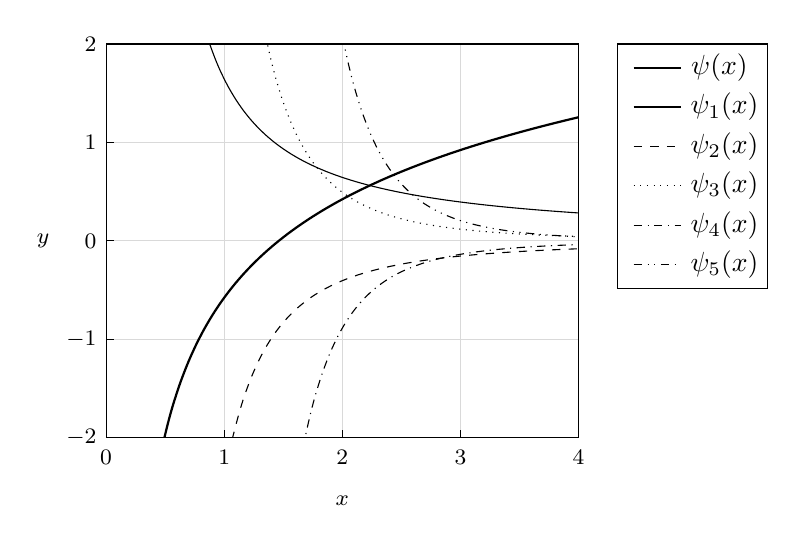
\begin{tikzpicture}
        \begin{scope}[every node/.append style = {font = \footnotesize}]
            \foreach \x in {0, ..., 4}
                \node at (6*\x/4,-2.75) {$\x$};
            \foreach \x in {1, 2, 3} {
                \draw[style = thin, gray!30!white] (6*\x/4,-2.5) -- (6*\x/4,2.5);
                \draw (6*\x/4,-2.5) -- (6*\x/4,-2.4);
            }
            \foreach \y in {-2, ..., 2}
                \node[anchor = east] at (0,2.5*\y/2) {$\y$};
            \foreach \y in {-1, 0, 1} {
                \draw[style = thin, gray!30!white] (0,2.5*\y/2) -- (6,2.5*\y/2);
                \draw (0,2.5*\y/2) -- (0.1,2.5*\y/2);
            }
            \node at (3,-3.3) {$x$};
            \node at (-0.8,0) {$y$};
        \end{scope}
        \begin{scope}
        \draw[clip] (0,-2.5) -- (6,-2.5) -- (6,2.5) -- (0,2.5) -- cycle;
        \draw[style = thick] plot[smooth, tension = 0.7] coordinates{(0.7,-2.6725) (0.8,-2.25975) (0.9,-1.92577) (1,-1.64779) (1.1,-1.41122) (1.2,-1.20626) (1.3,-1.02607) (1.4,-0.865704) (1.5,-0.72152) (1.6,-0.590743) (1.7,-0.471232) (1.8,-0.3613) (1.9,-0.2596) (2,-0.165042) (2.1,-0.0767307) (2.2,0.00607572) (2.3,0.0839977) (2.4,0.157559) (2.5,0.227207) (2.6,0.293323) (2.7,0.356239) (2.8,0.416242) (2.9,0.473582) (3,0.52848) (3.1,0.581132) (3.2,0.631709) (3.3,0.680367) (3.4,0.727242) (3.5,0.772458) (3.6,0.816126) (3.7,0.858348) (3.8,0.899215) (3.9,0.938809) (4,0.977207) (4.1,1.01448) (4.2,1.05068) (4.3,1.08588) (4.4,1.12013) (4.5,1.15348) (4.6,1.18597) (4.7,1.21765) (4.8,1.24855) (4.9,1.27871) (5,1.30817) (5.1,1.33696) (5.2,1.36511) (5.3,1.39264) (5.4,1.41958) (5.5,1.44596) (5.6,1.47179) (5.7,1.49711) (5.8,1.52193) (5.9,1.54627) (6,1.57015)};
        \draw plot[smooth, tension = 0.7] coordinates{(1.3,2.54368) (1.4,2.27622) (1.5,2.05617) (1.6,1.87244) (1.7,1.71708) (1.8,1.58422) (1.9,1.46948) (2,1.3695) (2.1,1.2817) (2.2,1.20404) (2.3,1.13492) (2.4,1.07304) (2.5,1.01734) (2.6,0.966974) (2.7,0.921218) (2.8,0.879483) (2.9,0.841273) (3,0.806168) (3.1,0.773811) (3.2,0.743898) (3.3,0.716166) (3.4,0.690389) (3.5,0.666371) (3.6,0.643941) (3.7,0.622947) (3.8,0.603258) (3.9,0.584759) (4,0.567344) (4.1,0.550924) (4.2,0.535415) (4.3,0.520746) (4.4,0.506849) (4.5,0.493668) (4.6,0.481147) (4.7,0.469239) (4.8,0.457901) (4.9,0.447094) (5,0.43678) (5.1,0.426927) (5.2,0.417505) (5.3,0.408487) (5.4,0.399847) (5.5,0.391563) (5.6,0.383613) (5.7,0.375976) (5.8,0.368636) (5.9,0.361576) (6,0.354779)};
        \draw[style = dashed] plot[smooth, tension = 0.7] coordinates{(1.6,-2.52626) (1.7,-2.14911) (1.8,-1.84755) (1.9,-1.60314) (2,-1.40265) (2.1,-1.23641) (2.2,-1.09721) (2.3,-0.979613) (2.4,-0.879465) (2.5,-0.793546) (2.6,-0.719333) (2.7,-0.654832) (2.8,-0.598449) (2.9,-0.548901) (3,-0.505142) (3.1,-0.46632) (3.2,-0.431729) (3.3,-0.400786) (3.4,-0.373001) (3.5,-0.347965) (3.6,-0.325332) (3.7,-0.304807) (3.8,-0.286139) (3.9,-0.269114) (4,-0.253546) (4.1,-0.239275) (4.2,-0.226163) (4.3,-0.214088) (4.4,-0.202946) (4.5,-0.192642) (4.6,-0.183097) (4.7,-0.174237) (4.8,-0.166) (4.9,-0.158329) (5,-0.151172) (5.1,-0.144487) (5.2,-0.138232) (5.3,-0.132372) (5.4,-0.126874) (5.5,-0.12171) (5.6,-0.116852) (5.7,-0.112278) (5.8,-0.107965) (5.9,-0.103895) (6,-0.10005)};
        \draw[style = dotted] plot[smooth, tension = 0.7] coordinates{(2,2.72977) (2.1,2.27532) (2.2,1.91419) (2.3,1.624) (2.4,1.38843) (2.5,1.19542) (2.6,1.03592) (2.7,0.903068) (2.8,0.791606) (2.9,0.697454) (3,0.617424) (3.1,0.548999) (3.2,0.490175) (3.3,0.439345) (3.4,0.395214) (3.5,0.356724) (3.6,0.323012) (3.7,0.293368) (3.8,0.267201) (3.9,0.244022) (4,0.22342) (4.1,0.205049) (4.2,0.188619) (4.3,0.173882) (4.4,0.160627) (4.5,0.148674) (4.6,0.137868) (4.7,0.128076) (4.8,0.119183) (4.9,0.111088) (5,0.103704) (5.1,0.0969561) (5.2,0.090777) (5.3,0.0851085) (5.4,0.0798994) (5.5,0.0751041) (5.6,0.0706828) (5.7,0.0665997) (5.8,0.0628234) (5.9,0.0593258) (6,0.0560817)};
        \draw[style = dashdotted] plot[smooth, tension = 0.7] coordinates{(2.5,-2.6243) (2.6,-2.17772) (2.7,-1.82085) (2.8,-1.53315) (2.9,-1.29932) (3,-1.10783) (3.1,-0.949911) (3.2,-0.818808) (3.3,-0.709295) (3.4,-0.617285) (3.5,-0.539558) (3.6,-0.473559) (3.7,-0.417246) (3.8,-0.368976) (3.9,-0.327423) (4,-0.291503) (4.1,-0.260333) (4.2,-0.233184) (4.3,-0.209454) (4.4,-0.188642) (4.5,-0.170333) (4.6,-0.154175) (4.7,-0.139874) (4.8,-0.127182) (4.9,-0.115887) (5,-0.10581) (5.1,-0.0967987) (5.2,-0.0887202) (5.3,-0.081462) (5.4,-0.0749268) (5.5,-0.0690303) (5.6,-0.0636993) (5.7,-0.0588704) (5.8,-0.0544882) (5.9,-0.0505041) (6,-0.0468759)};
        \draw[style = dashdotdotted] plot[smooth, tension = 0.7] coordinates{(3,2.60146) (3.1,2.15294) (3.2,1.79313) (3.3,1.5024) (3.4,1.2659) (3.5,1.07227) (3.6,0.91279) (3.7,0.780693) (3.8,0.670687) (3.9,0.578612) (4,0.501173) (4.1,0.435747) (4.2,0.380228) (4.3,0.332923) (4.4,0.292456) (4.5,0.257709) (4.6,0.227767) (4.7,0.201876) (4.8,0.179416) (4.9,0.159869) (5,0.142808) (5.1,0.127873) (5.2,0.114763) (5.3,0.103224) (5.4,0.0930426) (5.5,0.0840363) (5.6,0.0760508) (5.7,0.0689543) (5.8,0.062634) (5.9,0.056993) (6,0.051948)};
        \end{scope}
        \draw (6.5,-0.6) -- (8.4,-0.6) -- (8.4,2.5) -- (6.5,2.5) -- cycle;
        \draw[style = thick] (6.7,2.2) -- (7.3,2.2) node[right] {$\psi(x)$};
        \draw (6.7,1.7) -- (7.3,1.7) node[right] {$\psi_1(x)$};
        \draw[style = dashed] (6.7,1.2) -- (7.3,1.2) node[right] {$\psi_2(x)$};
        \draw[style = dotted] (6.7,0.7) -- (7.3,0.7) node[right] {$\psi_3(x)$};
        \draw[style = dashdotted] (6.7,0.2) -- (7.3,0.2) node[right] {$\psi_4(x)$};
        \draw[style = dashdotdotted] (6.7,-0.3) -- (7.3,-0.3) node[right] {$\psi_5(x)$};
    \end{tikzpicture}
\end{figure}

\begin{figure}[!ht]
    \makebox[\linewidth][c]{
        \centering
        \subfigure{
            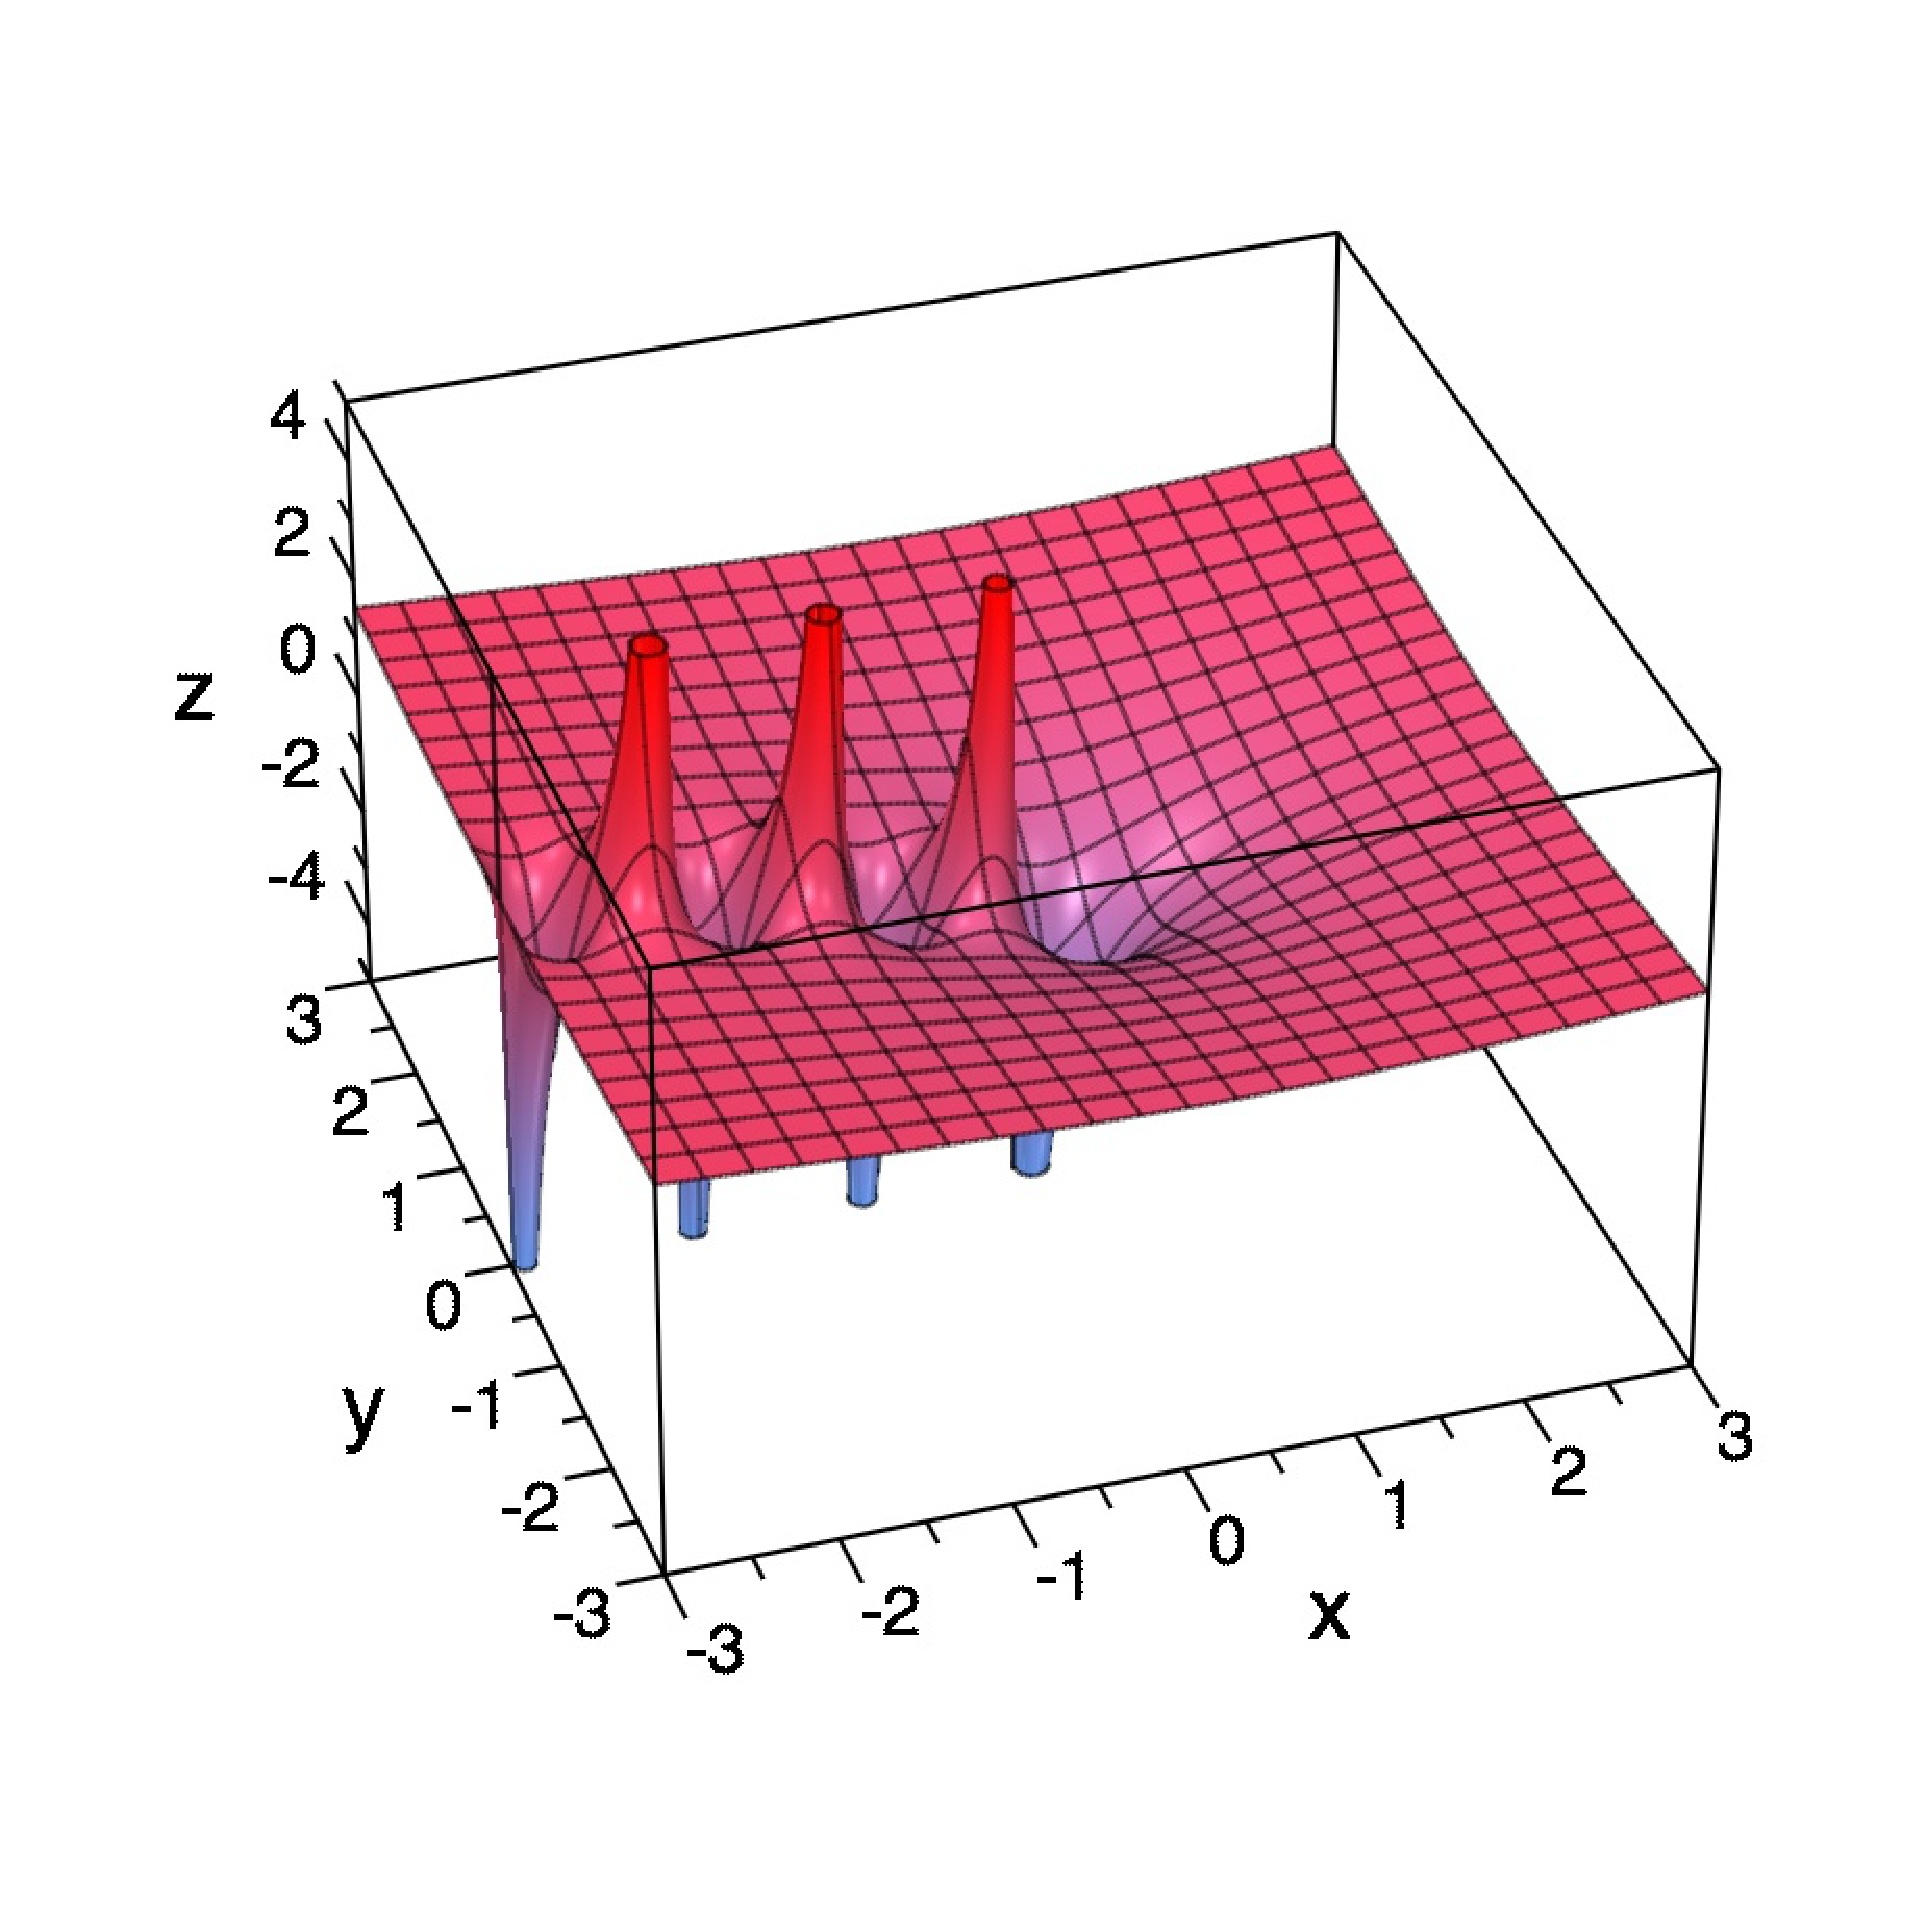
\includegraphics[width = 0.45\textwidth]{Psi0FuncRe.eps}
        }
        \subfigure{
            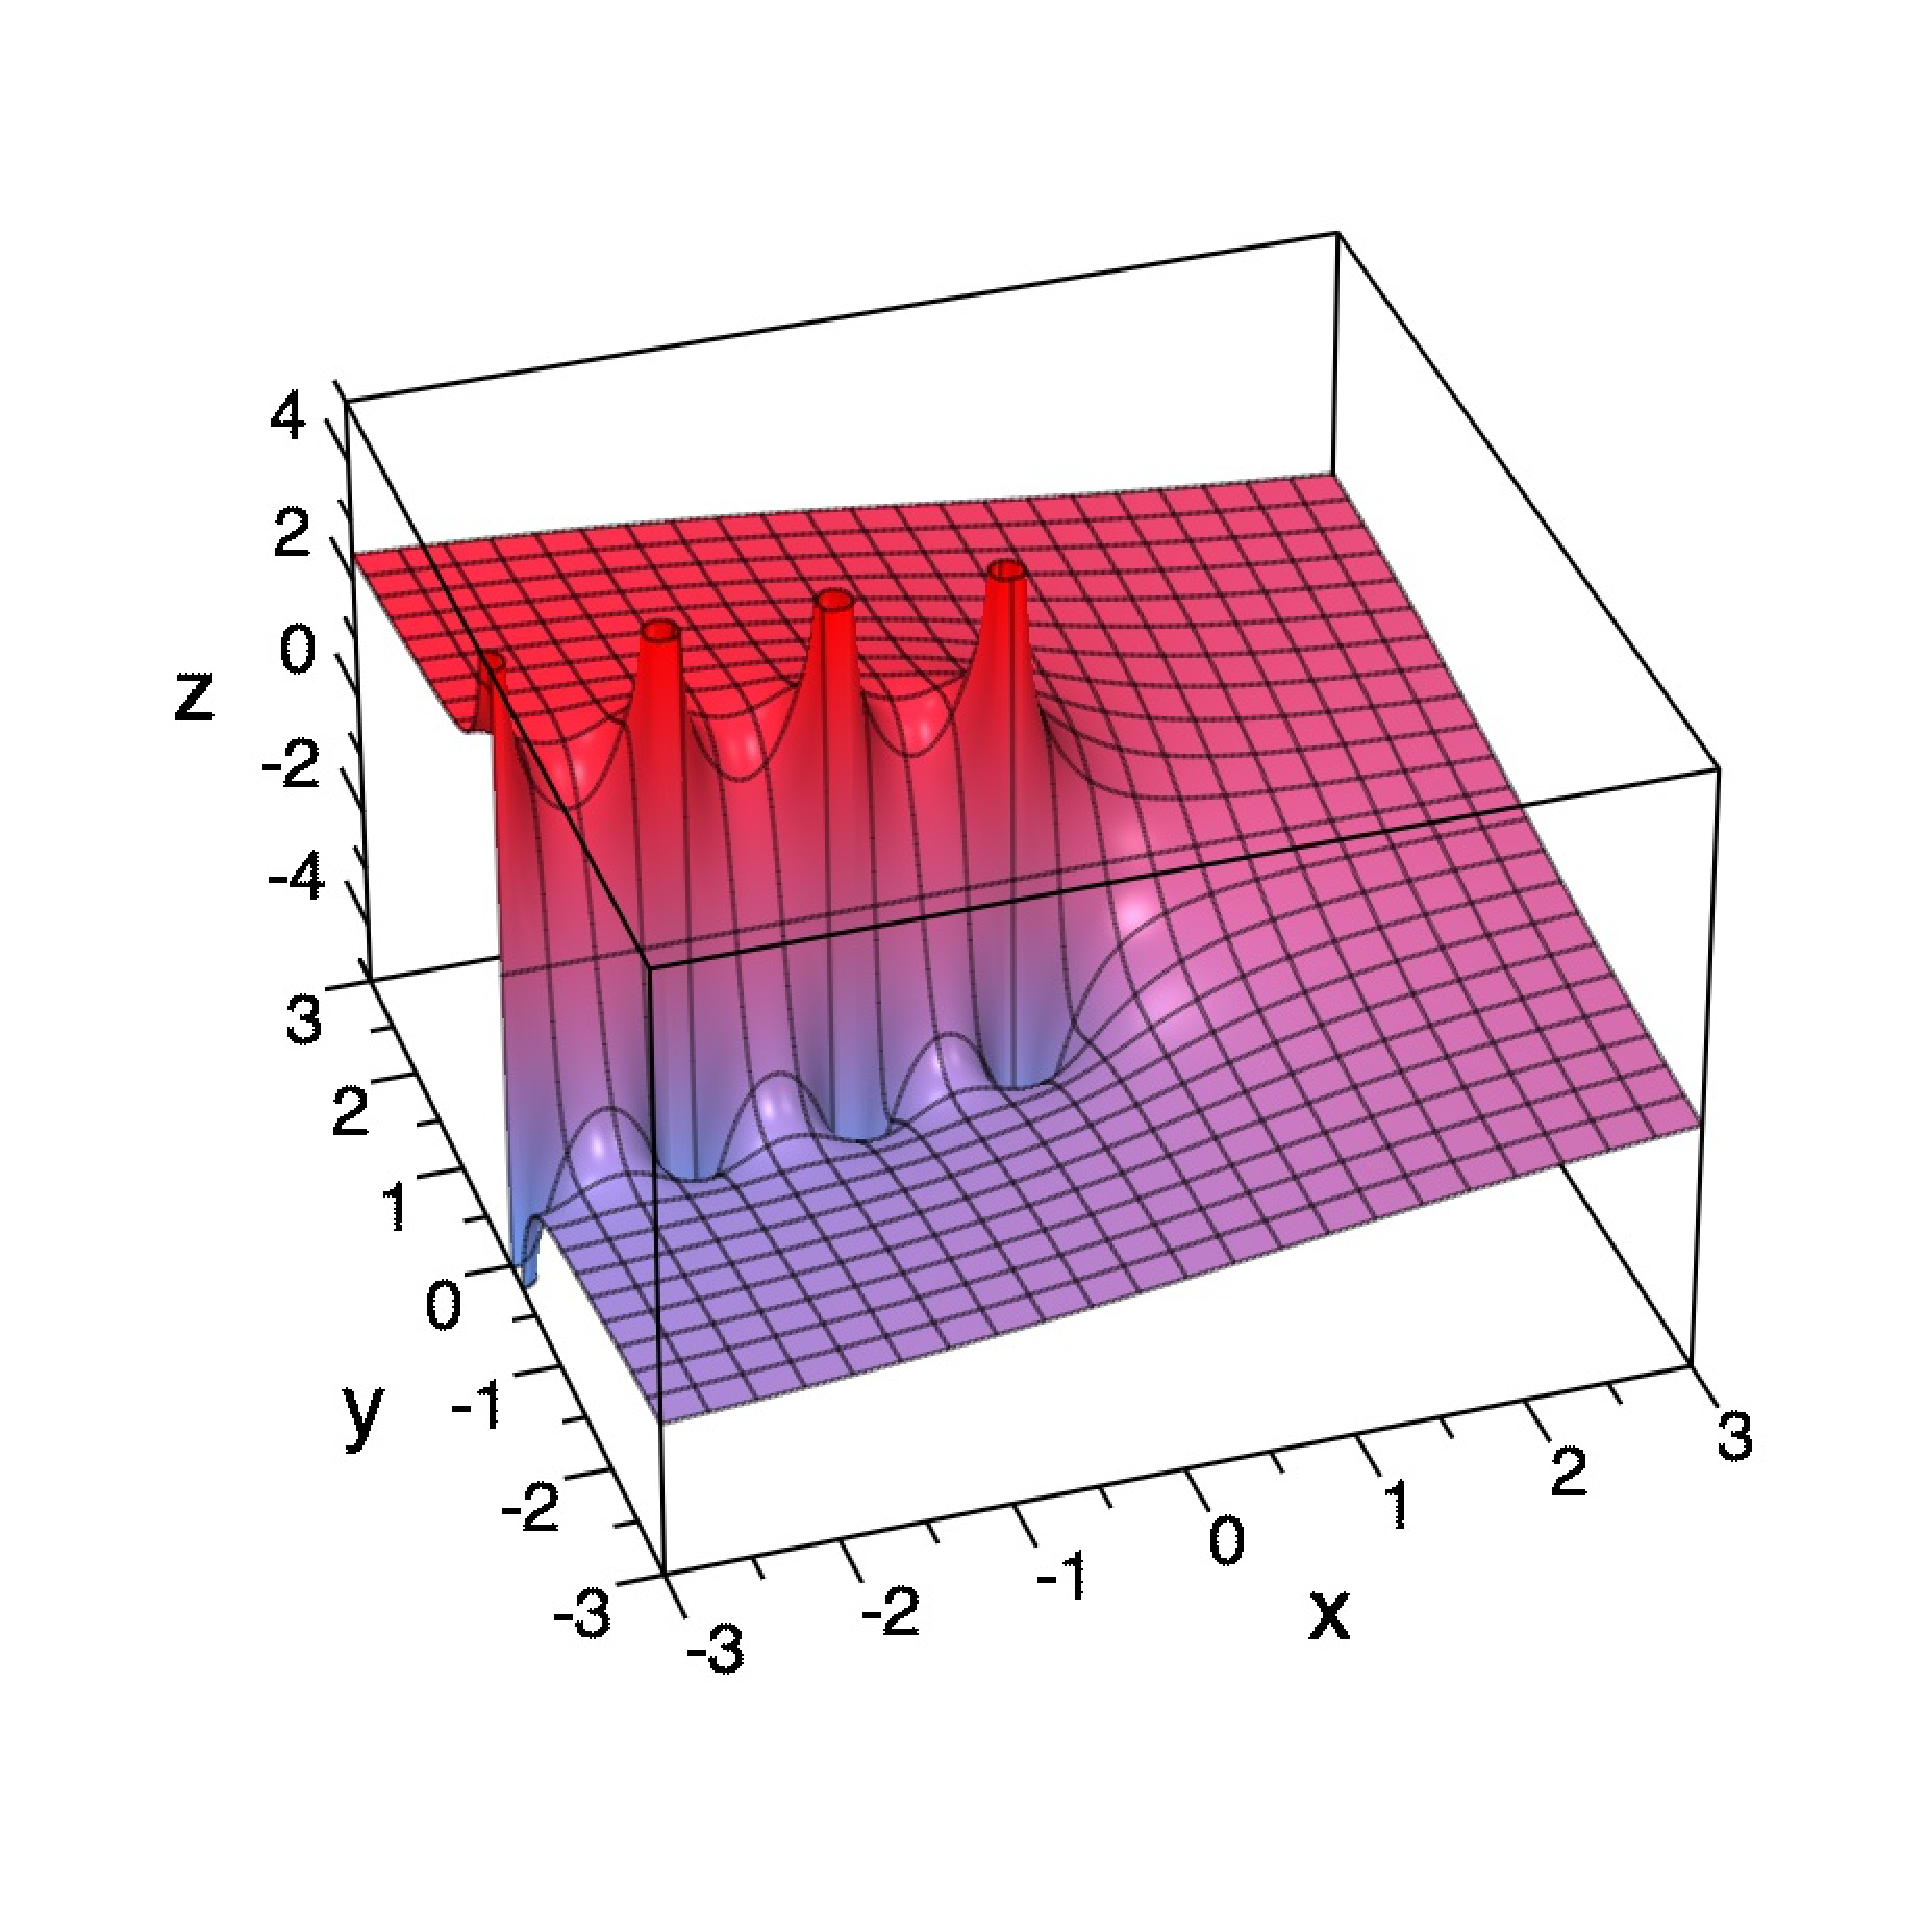
\includegraphics[width = 0.45\textwidth]{Psi0FuncIm.eps}
        }
        \subfigure{
            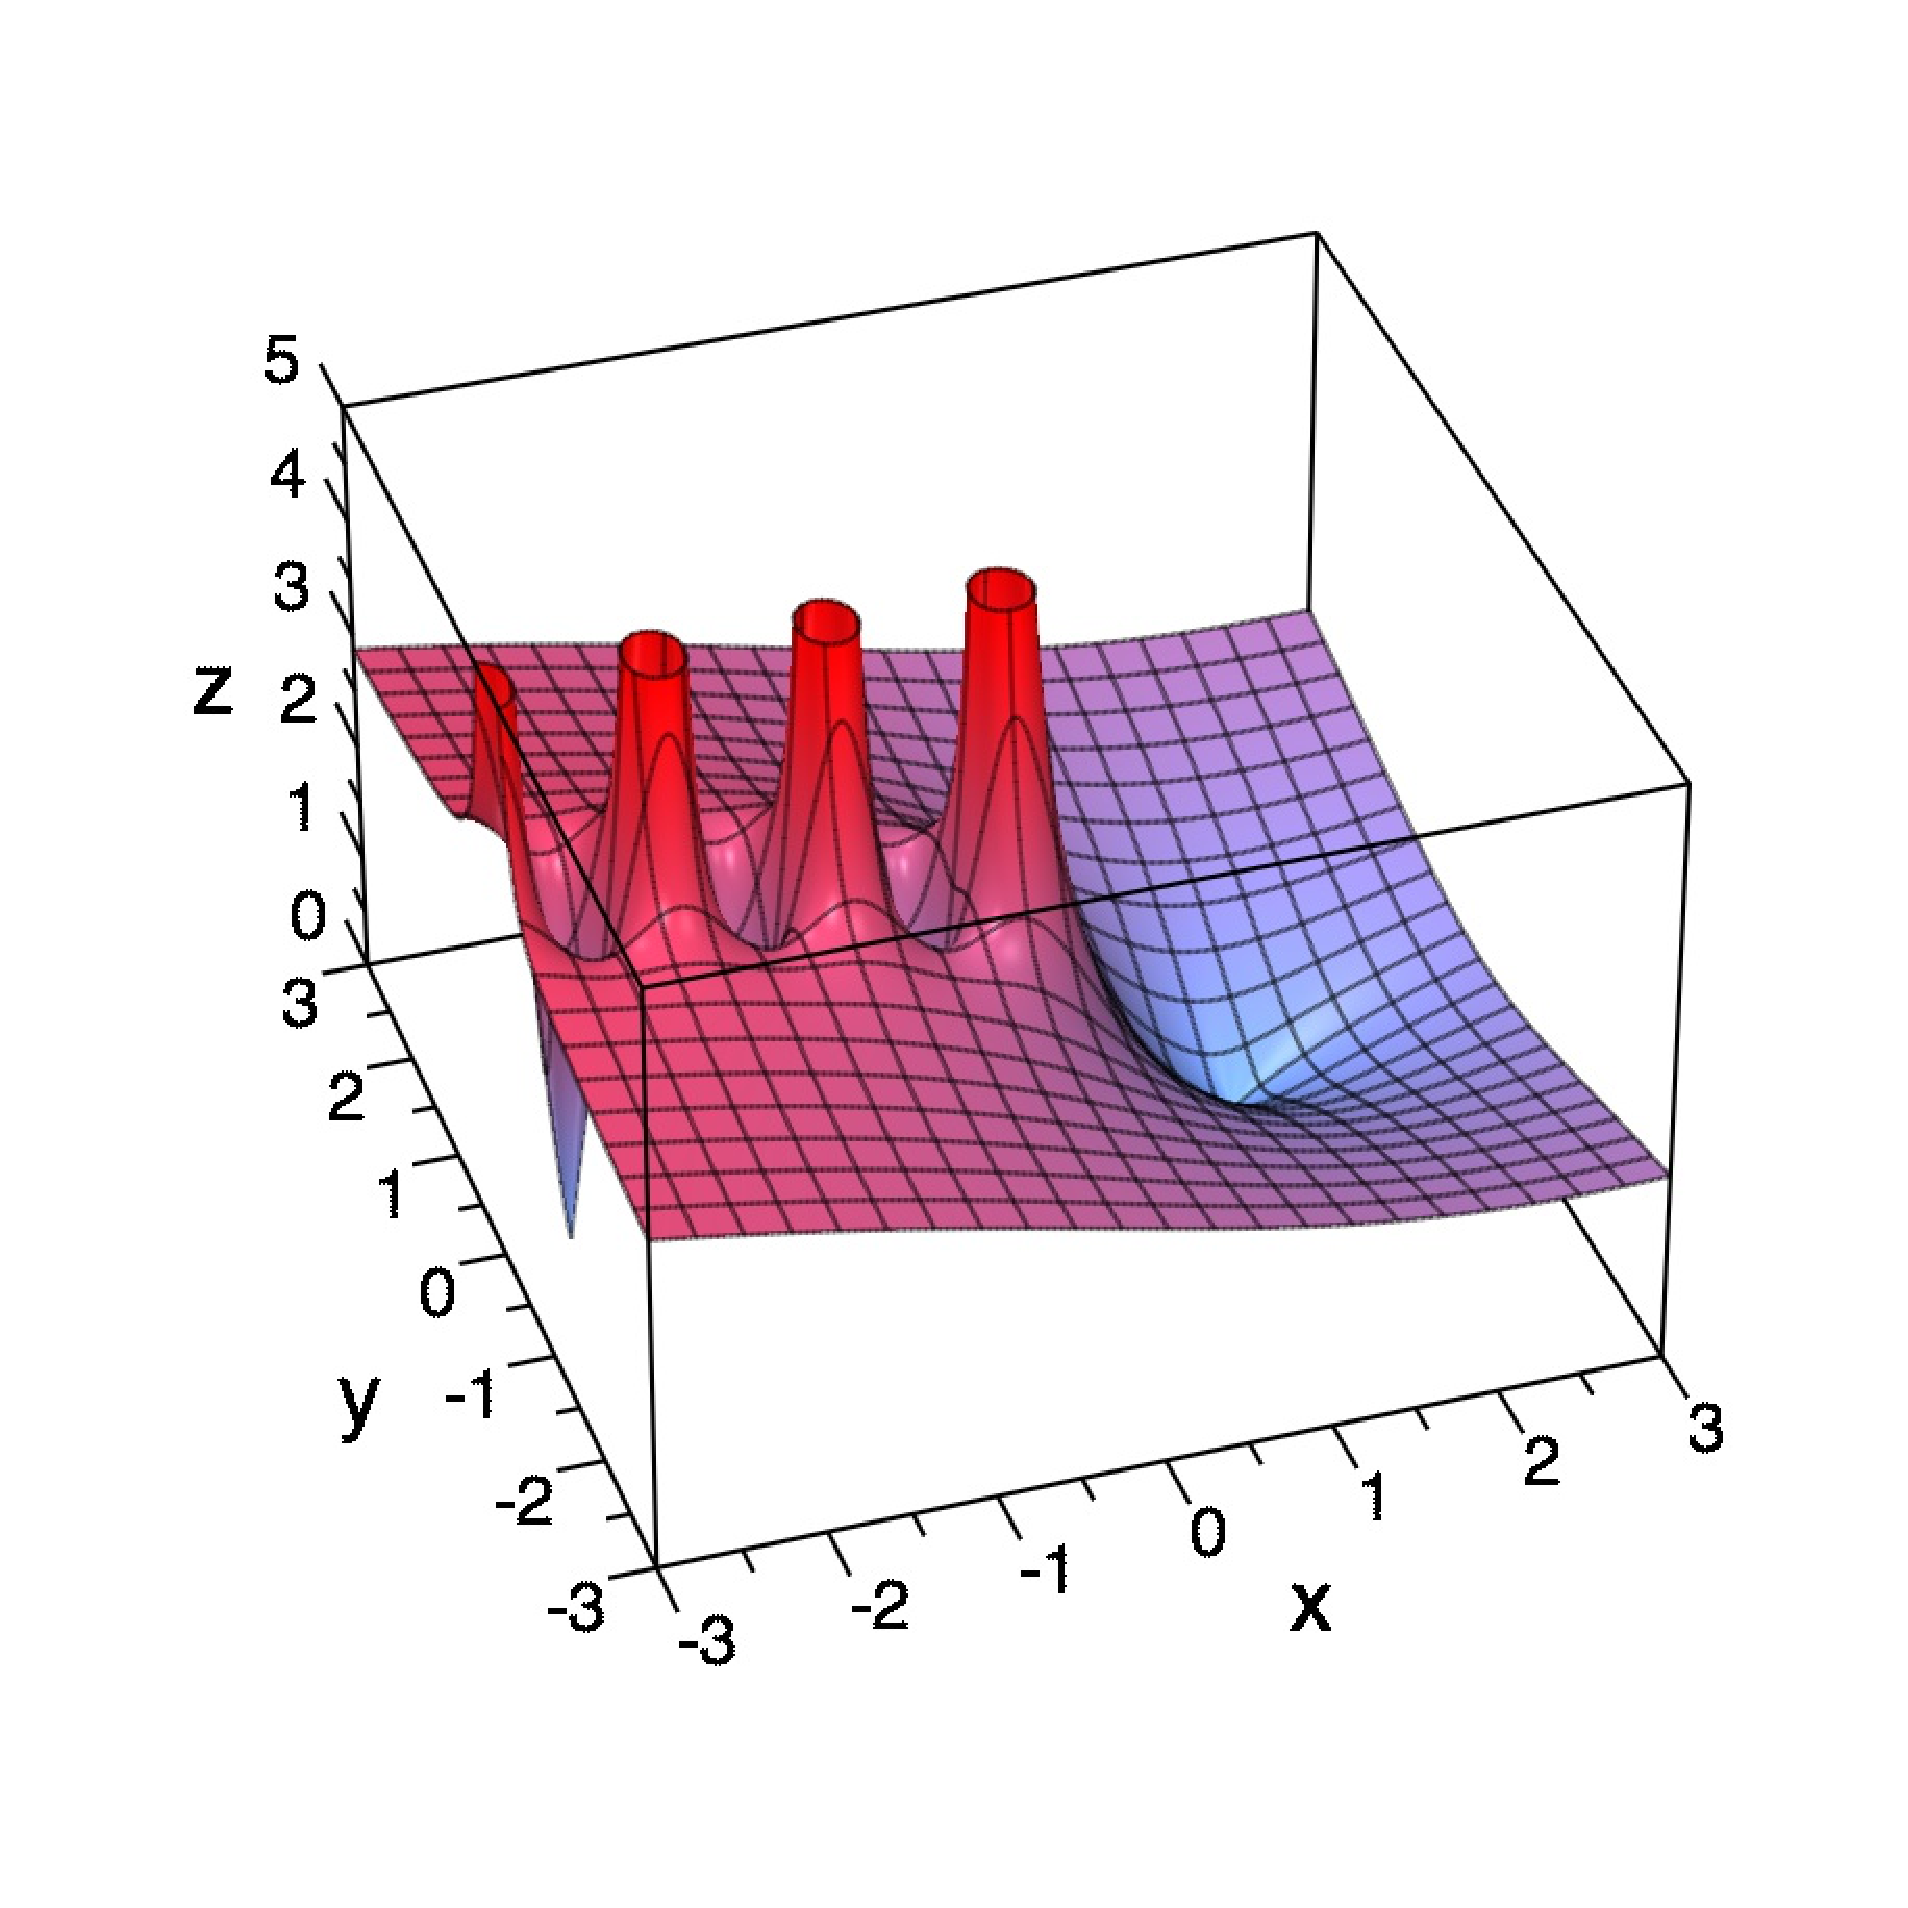
\includegraphics[width = 0.45\textwidth]{Psi0FuncAbs.eps}
        }
    }
\end{figure}

\begin{figure}[!ht]
    \makebox[\linewidth][c]{
        \centering
        \subfigure{
            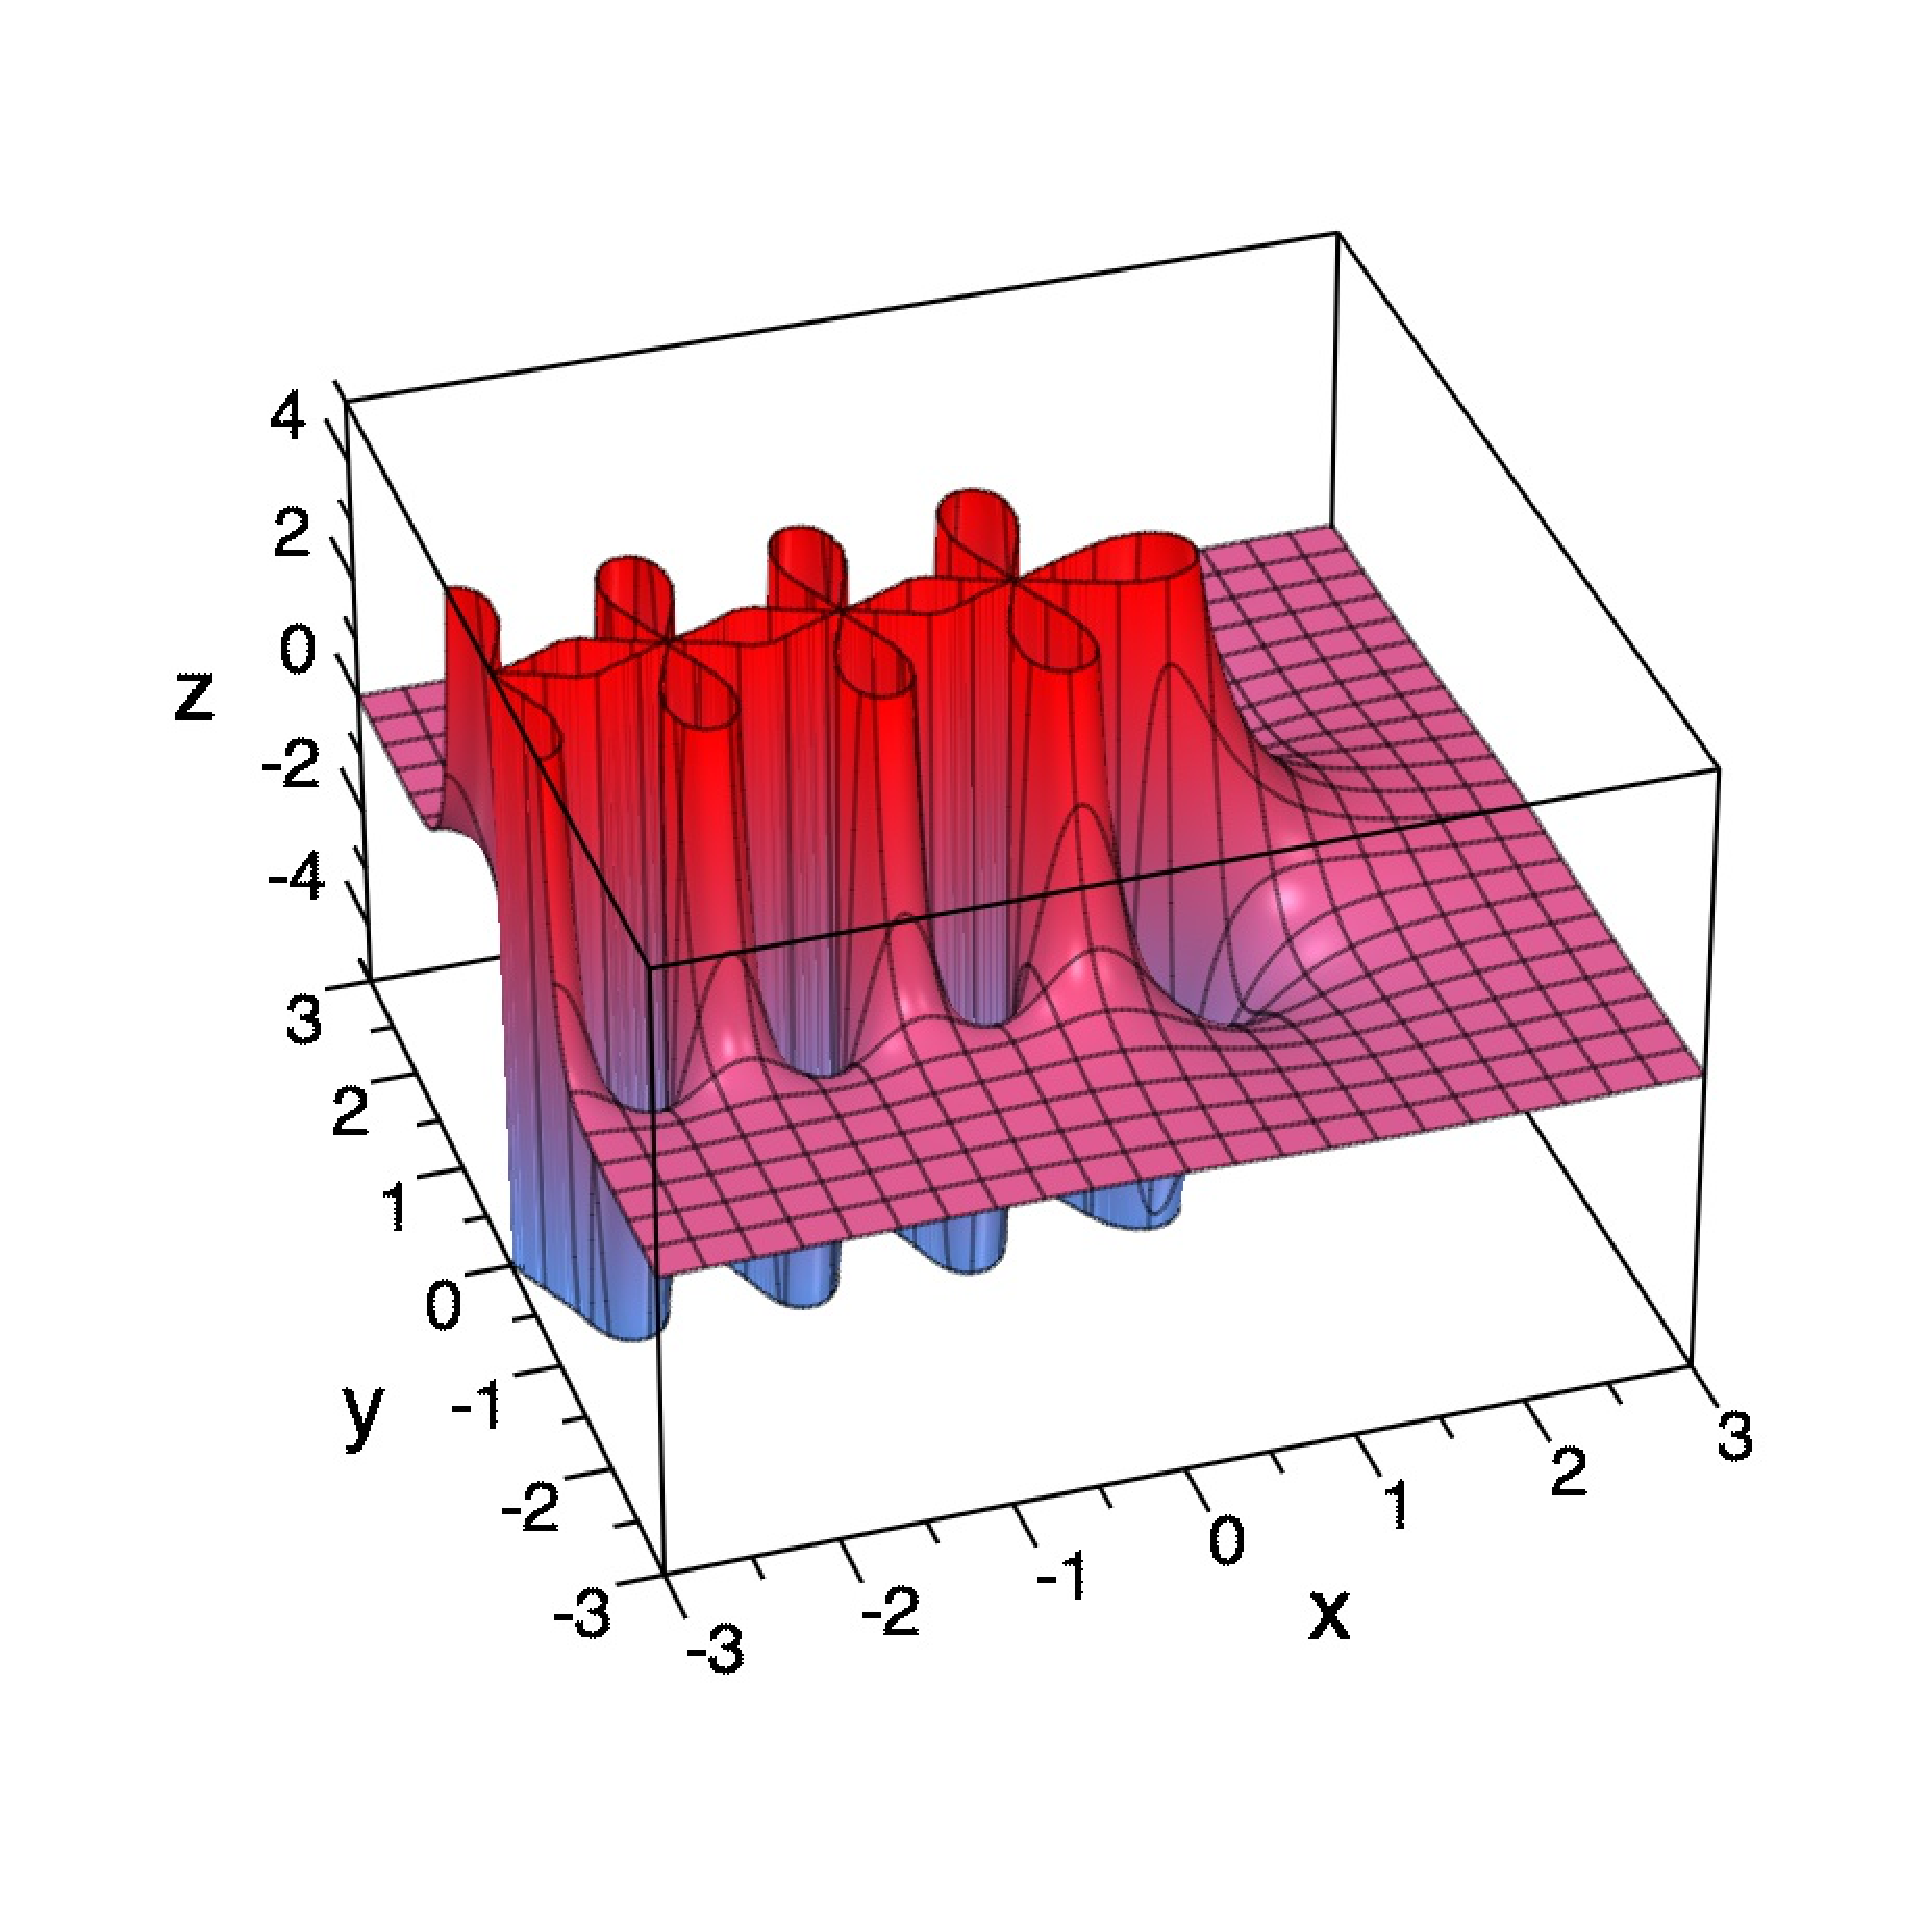
\includegraphics[width = 0.45\textwidth]{Psi3FuncRe.eps}
        }
        \subfigure{
            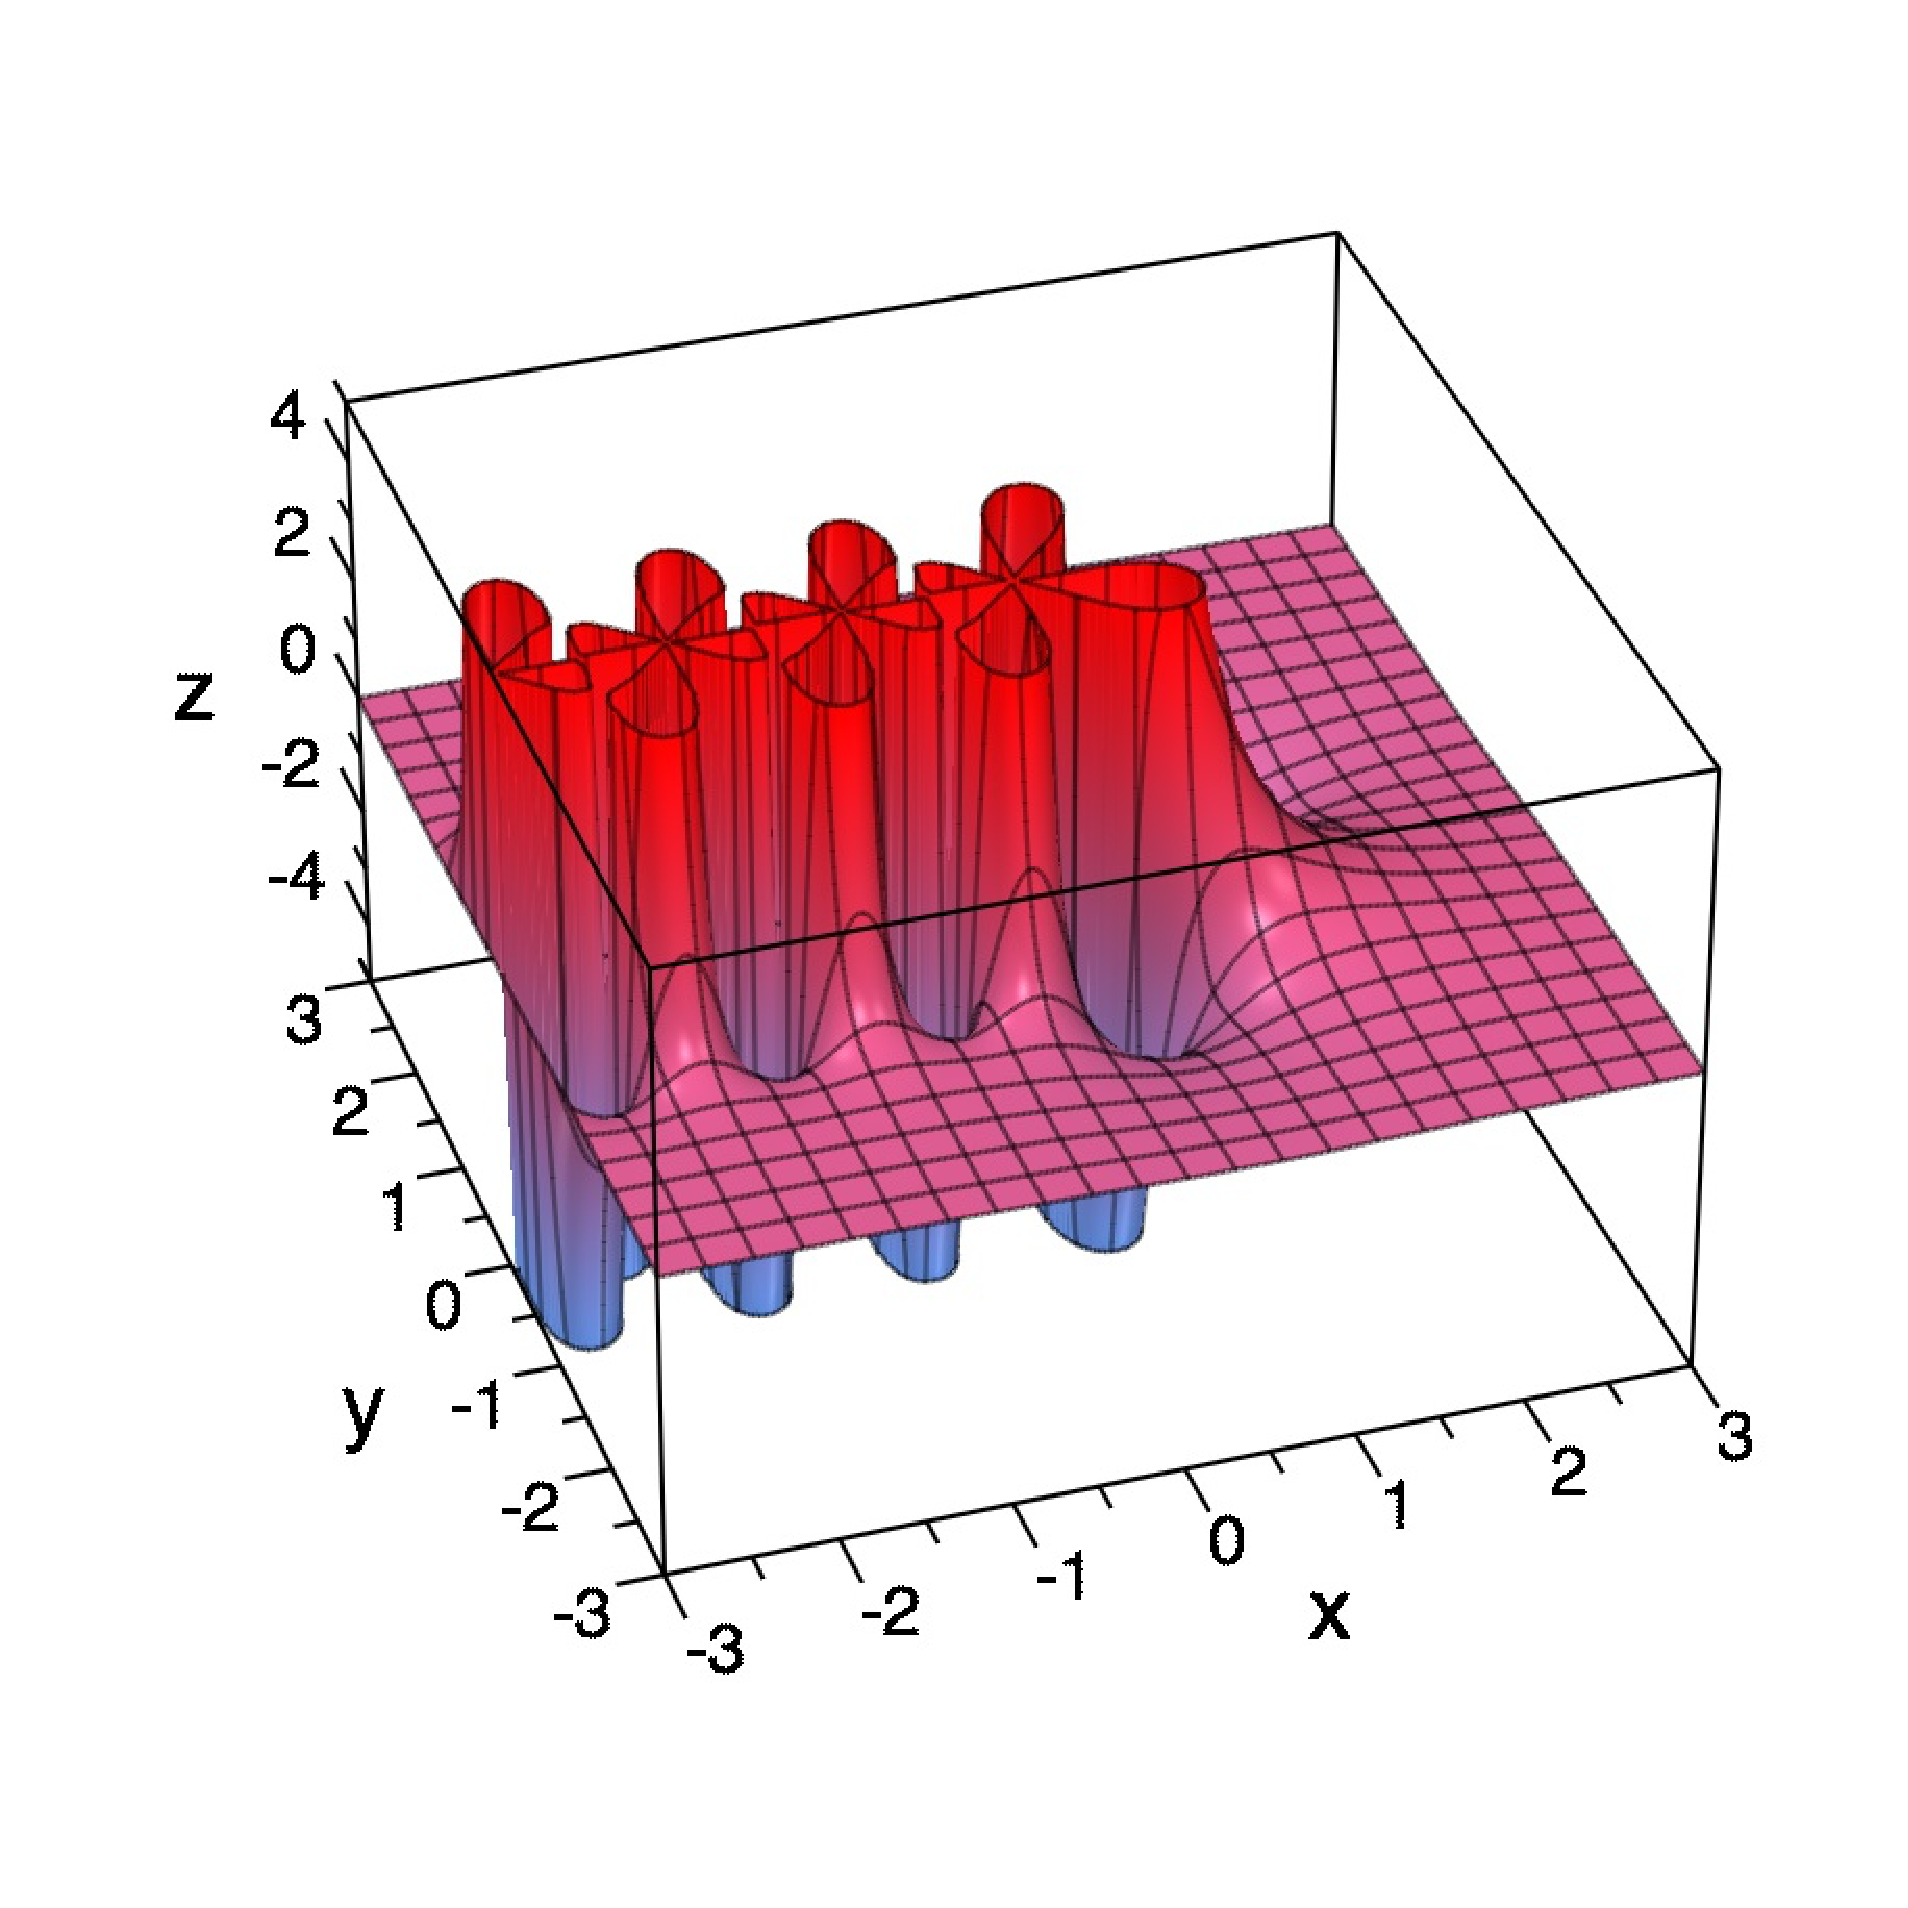
\includegraphics[width = 0.45\textwidth]{Psi3FuncIm.eps}
        }
        \subfigure{
            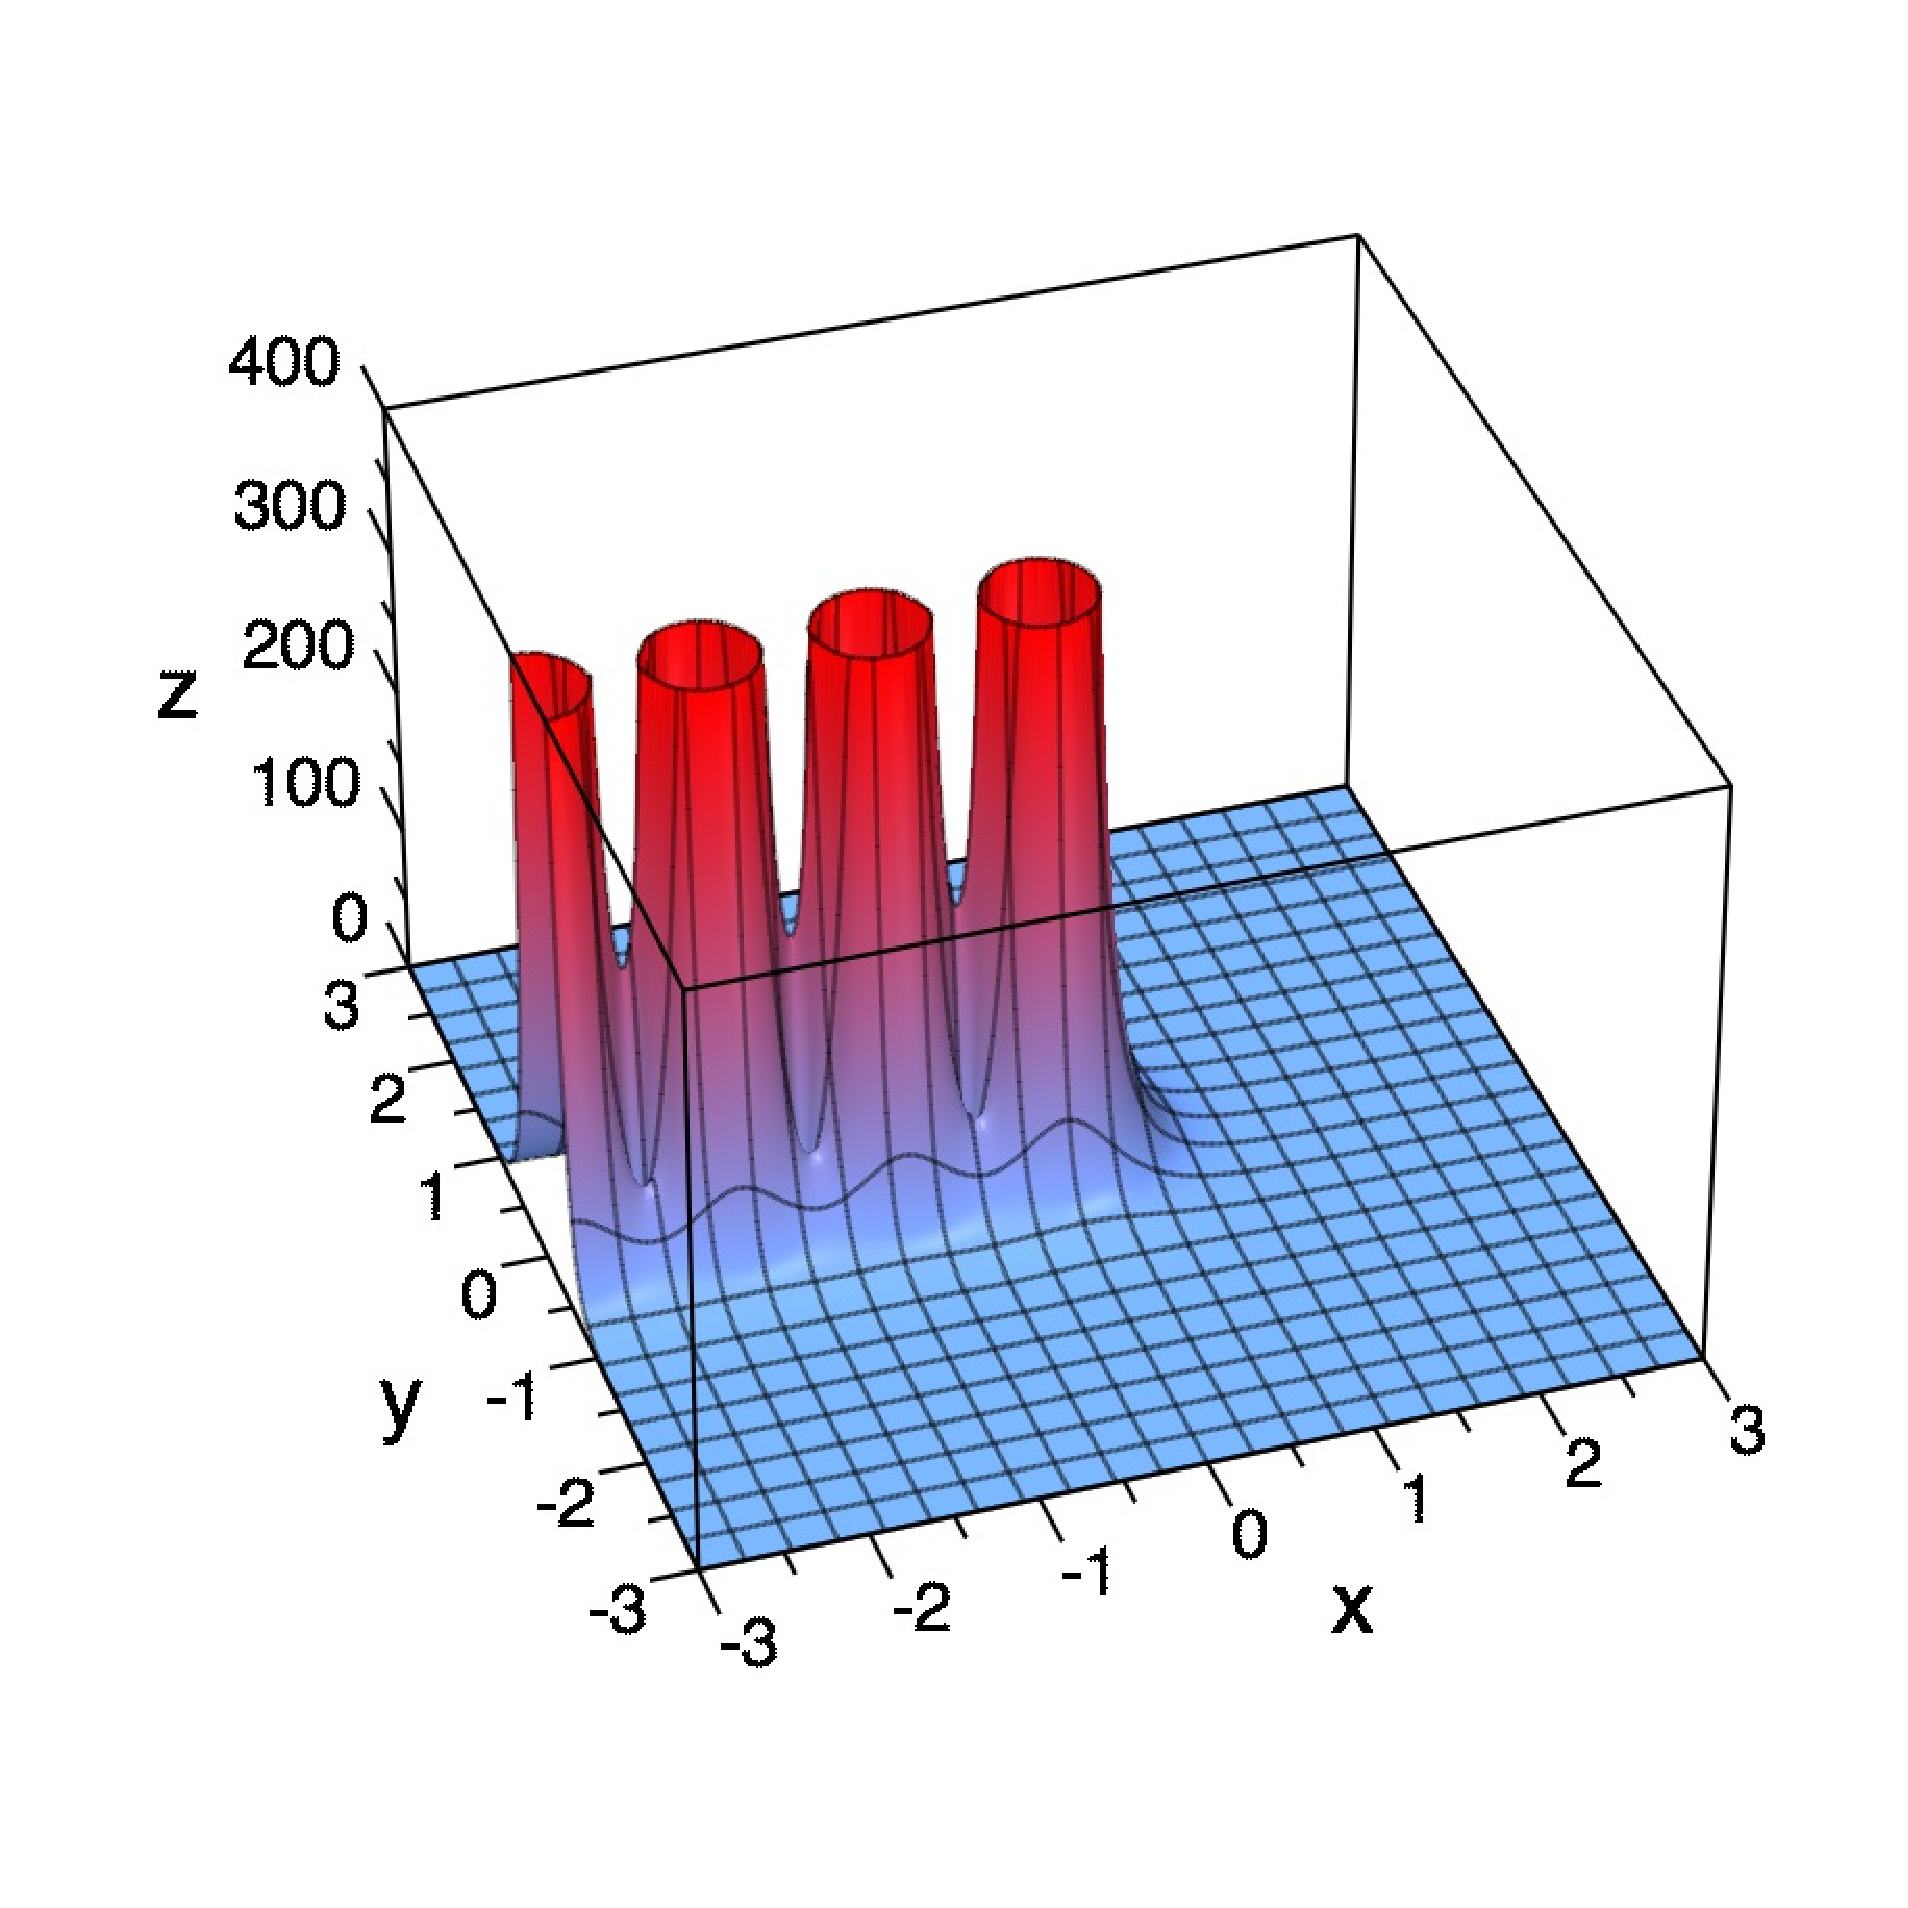
\includegraphics[width = 0.45\textwidth]{Psi3FuncAbs.eps}
        }
    }
\end{figure}

\begin{figure}[!ht]
    \makebox[\linewidth][c]{
        \centering
        \subfigure{
            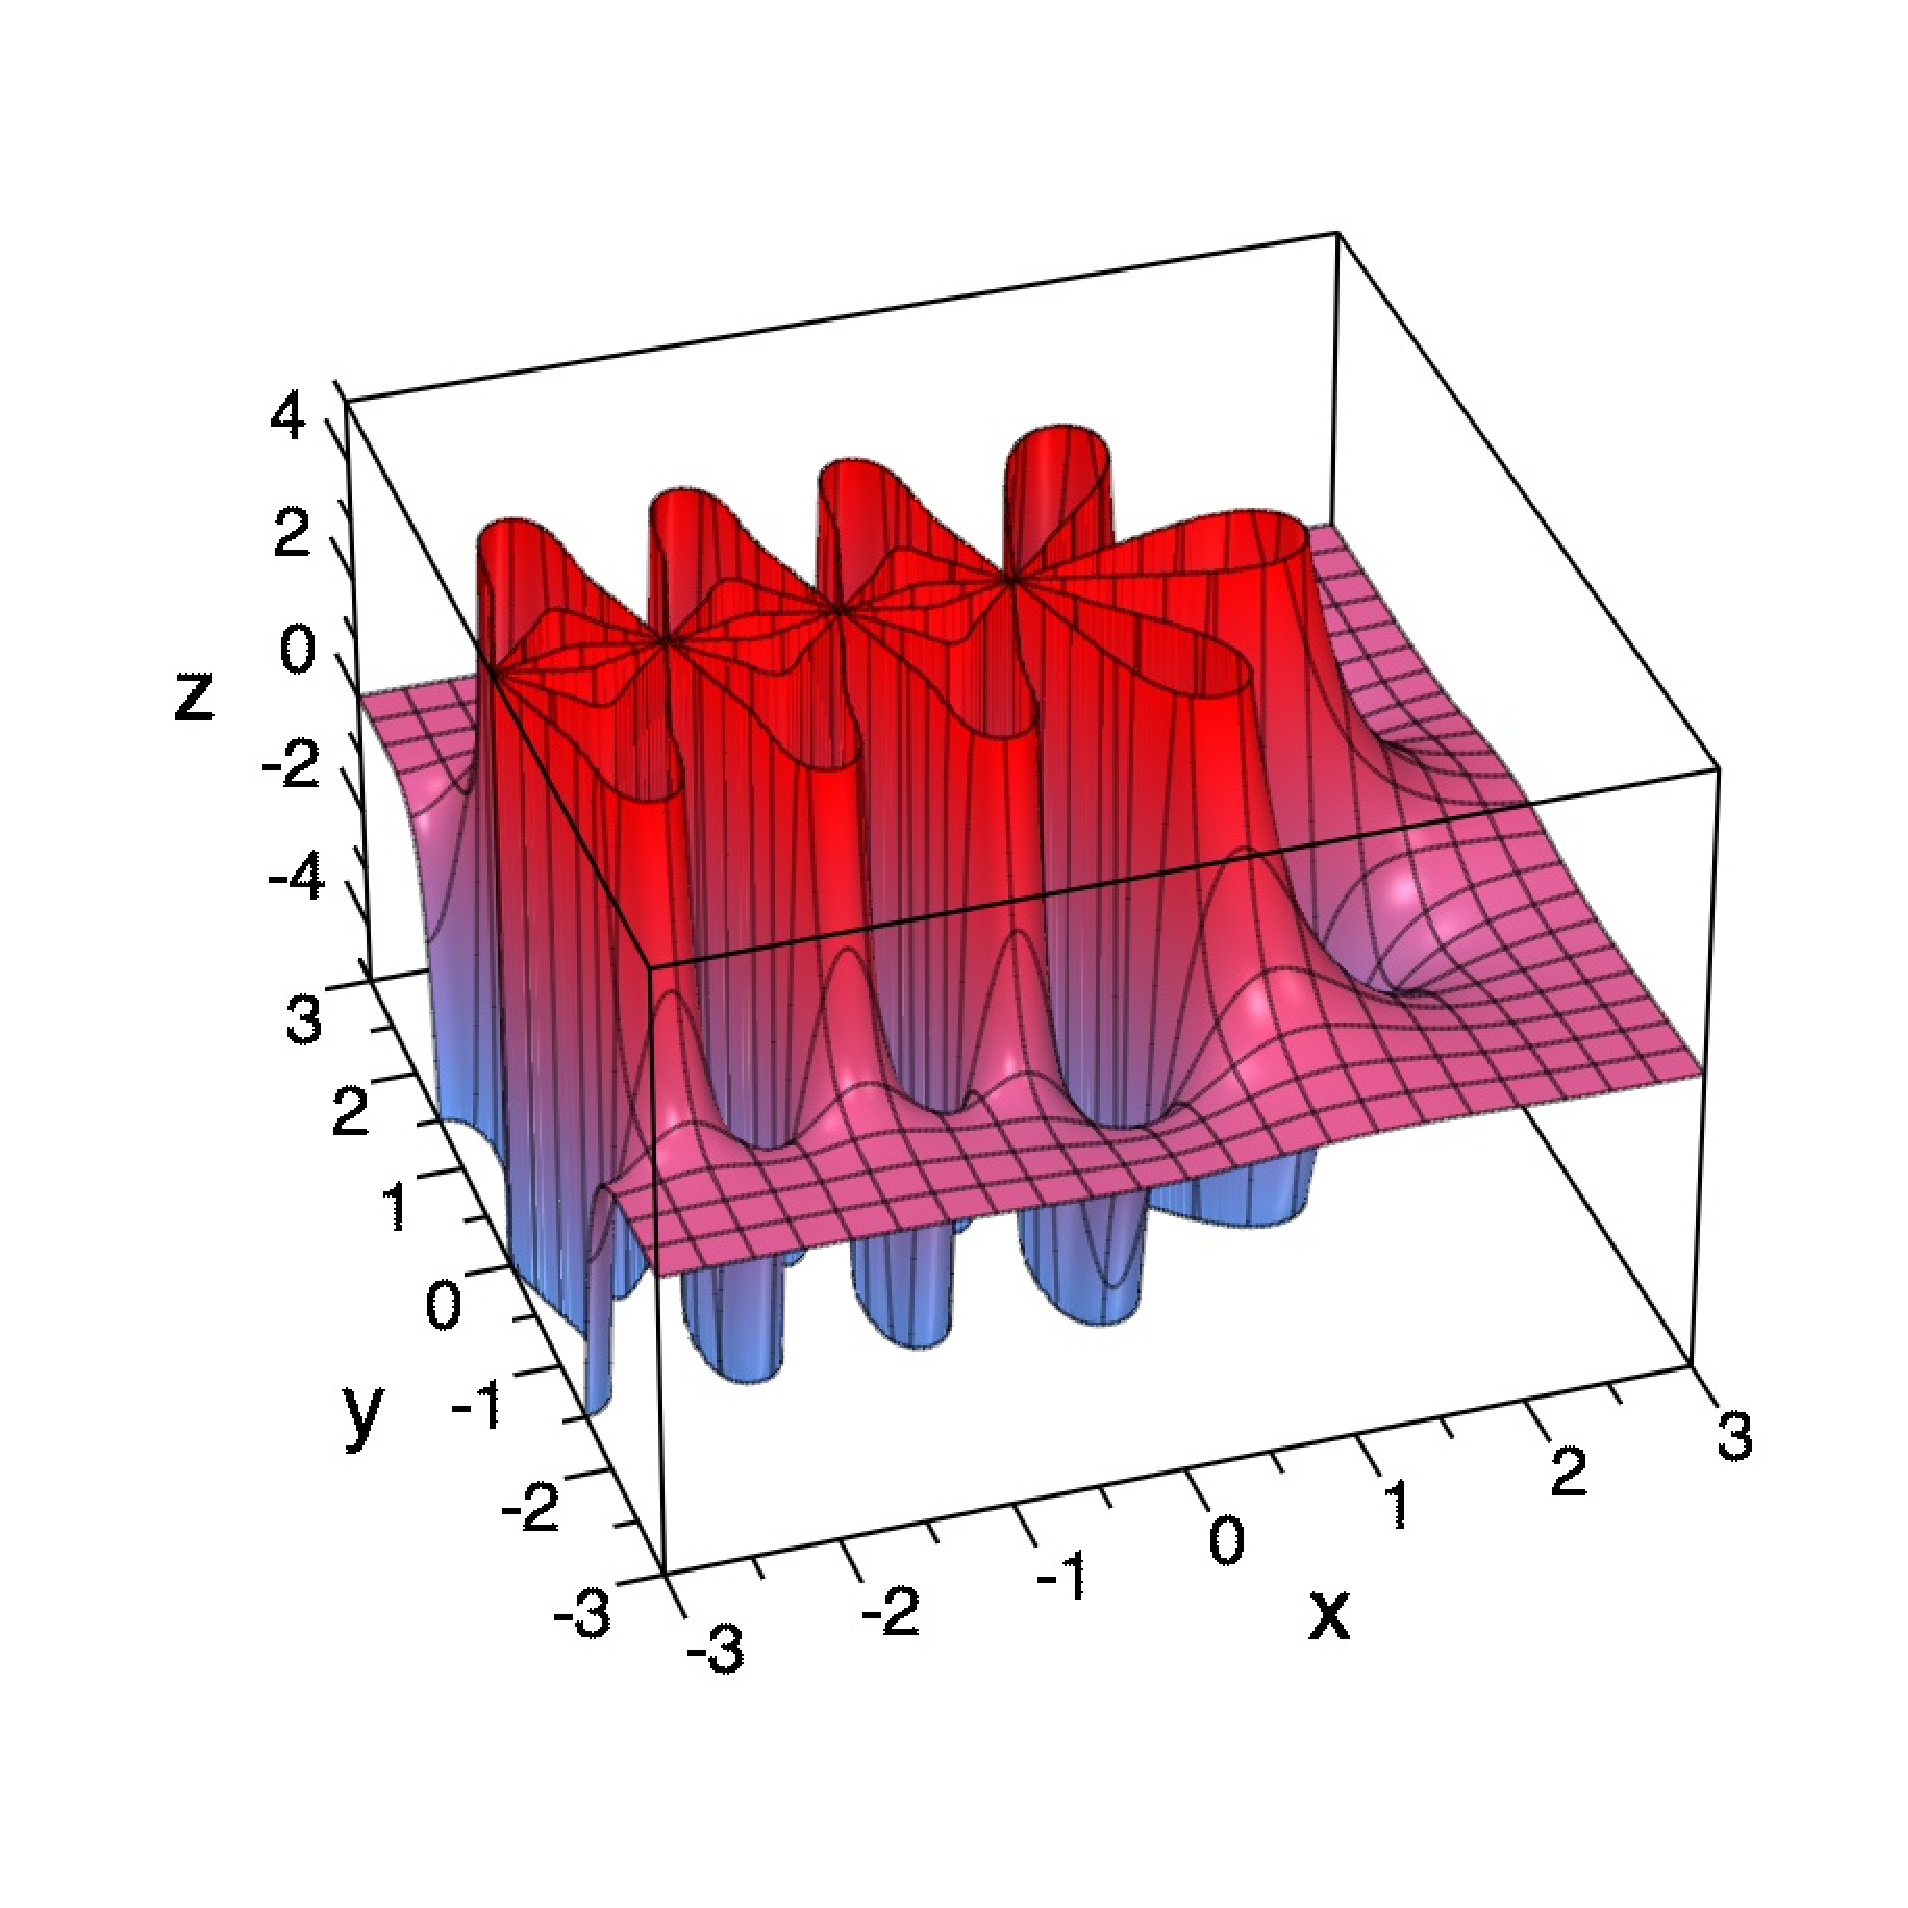
\includegraphics[width = 0.45\textwidth]{Psi5FuncRe.eps}
        }
        \subfigure{
            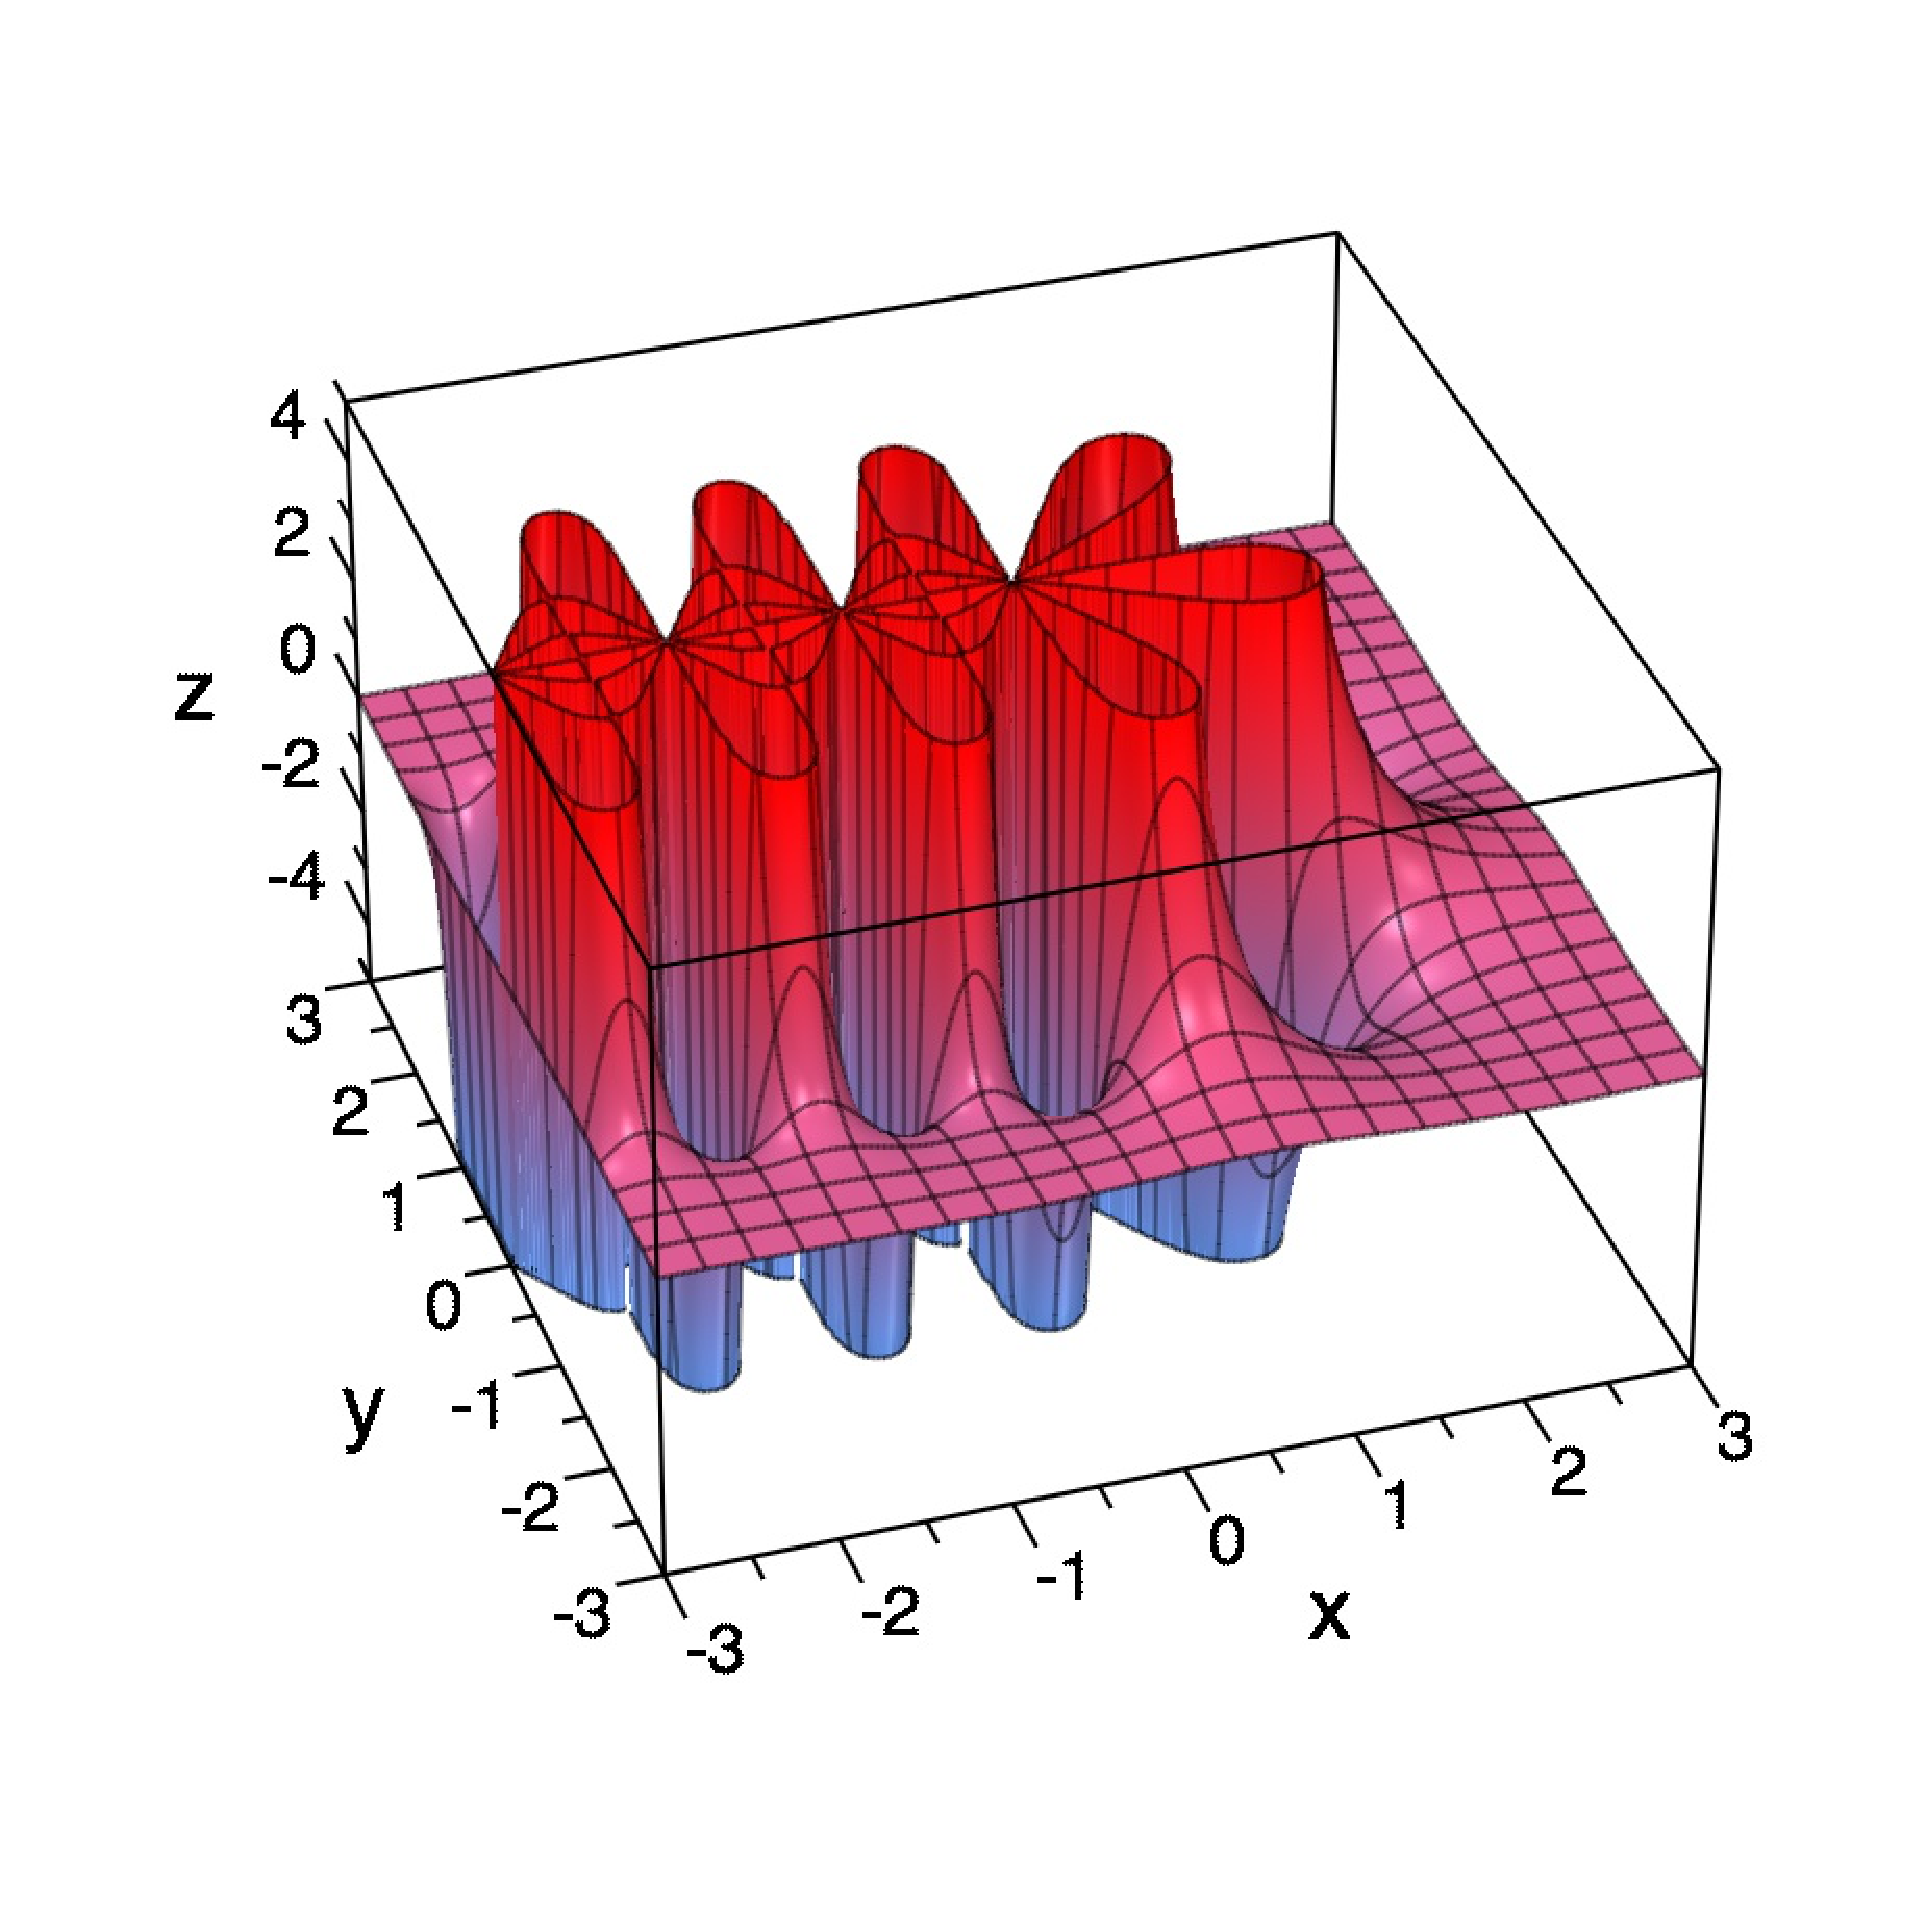
\includegraphics[width = 0.45\textwidth]{Psi5FuncIm.eps}
        }
        \subfigure{
            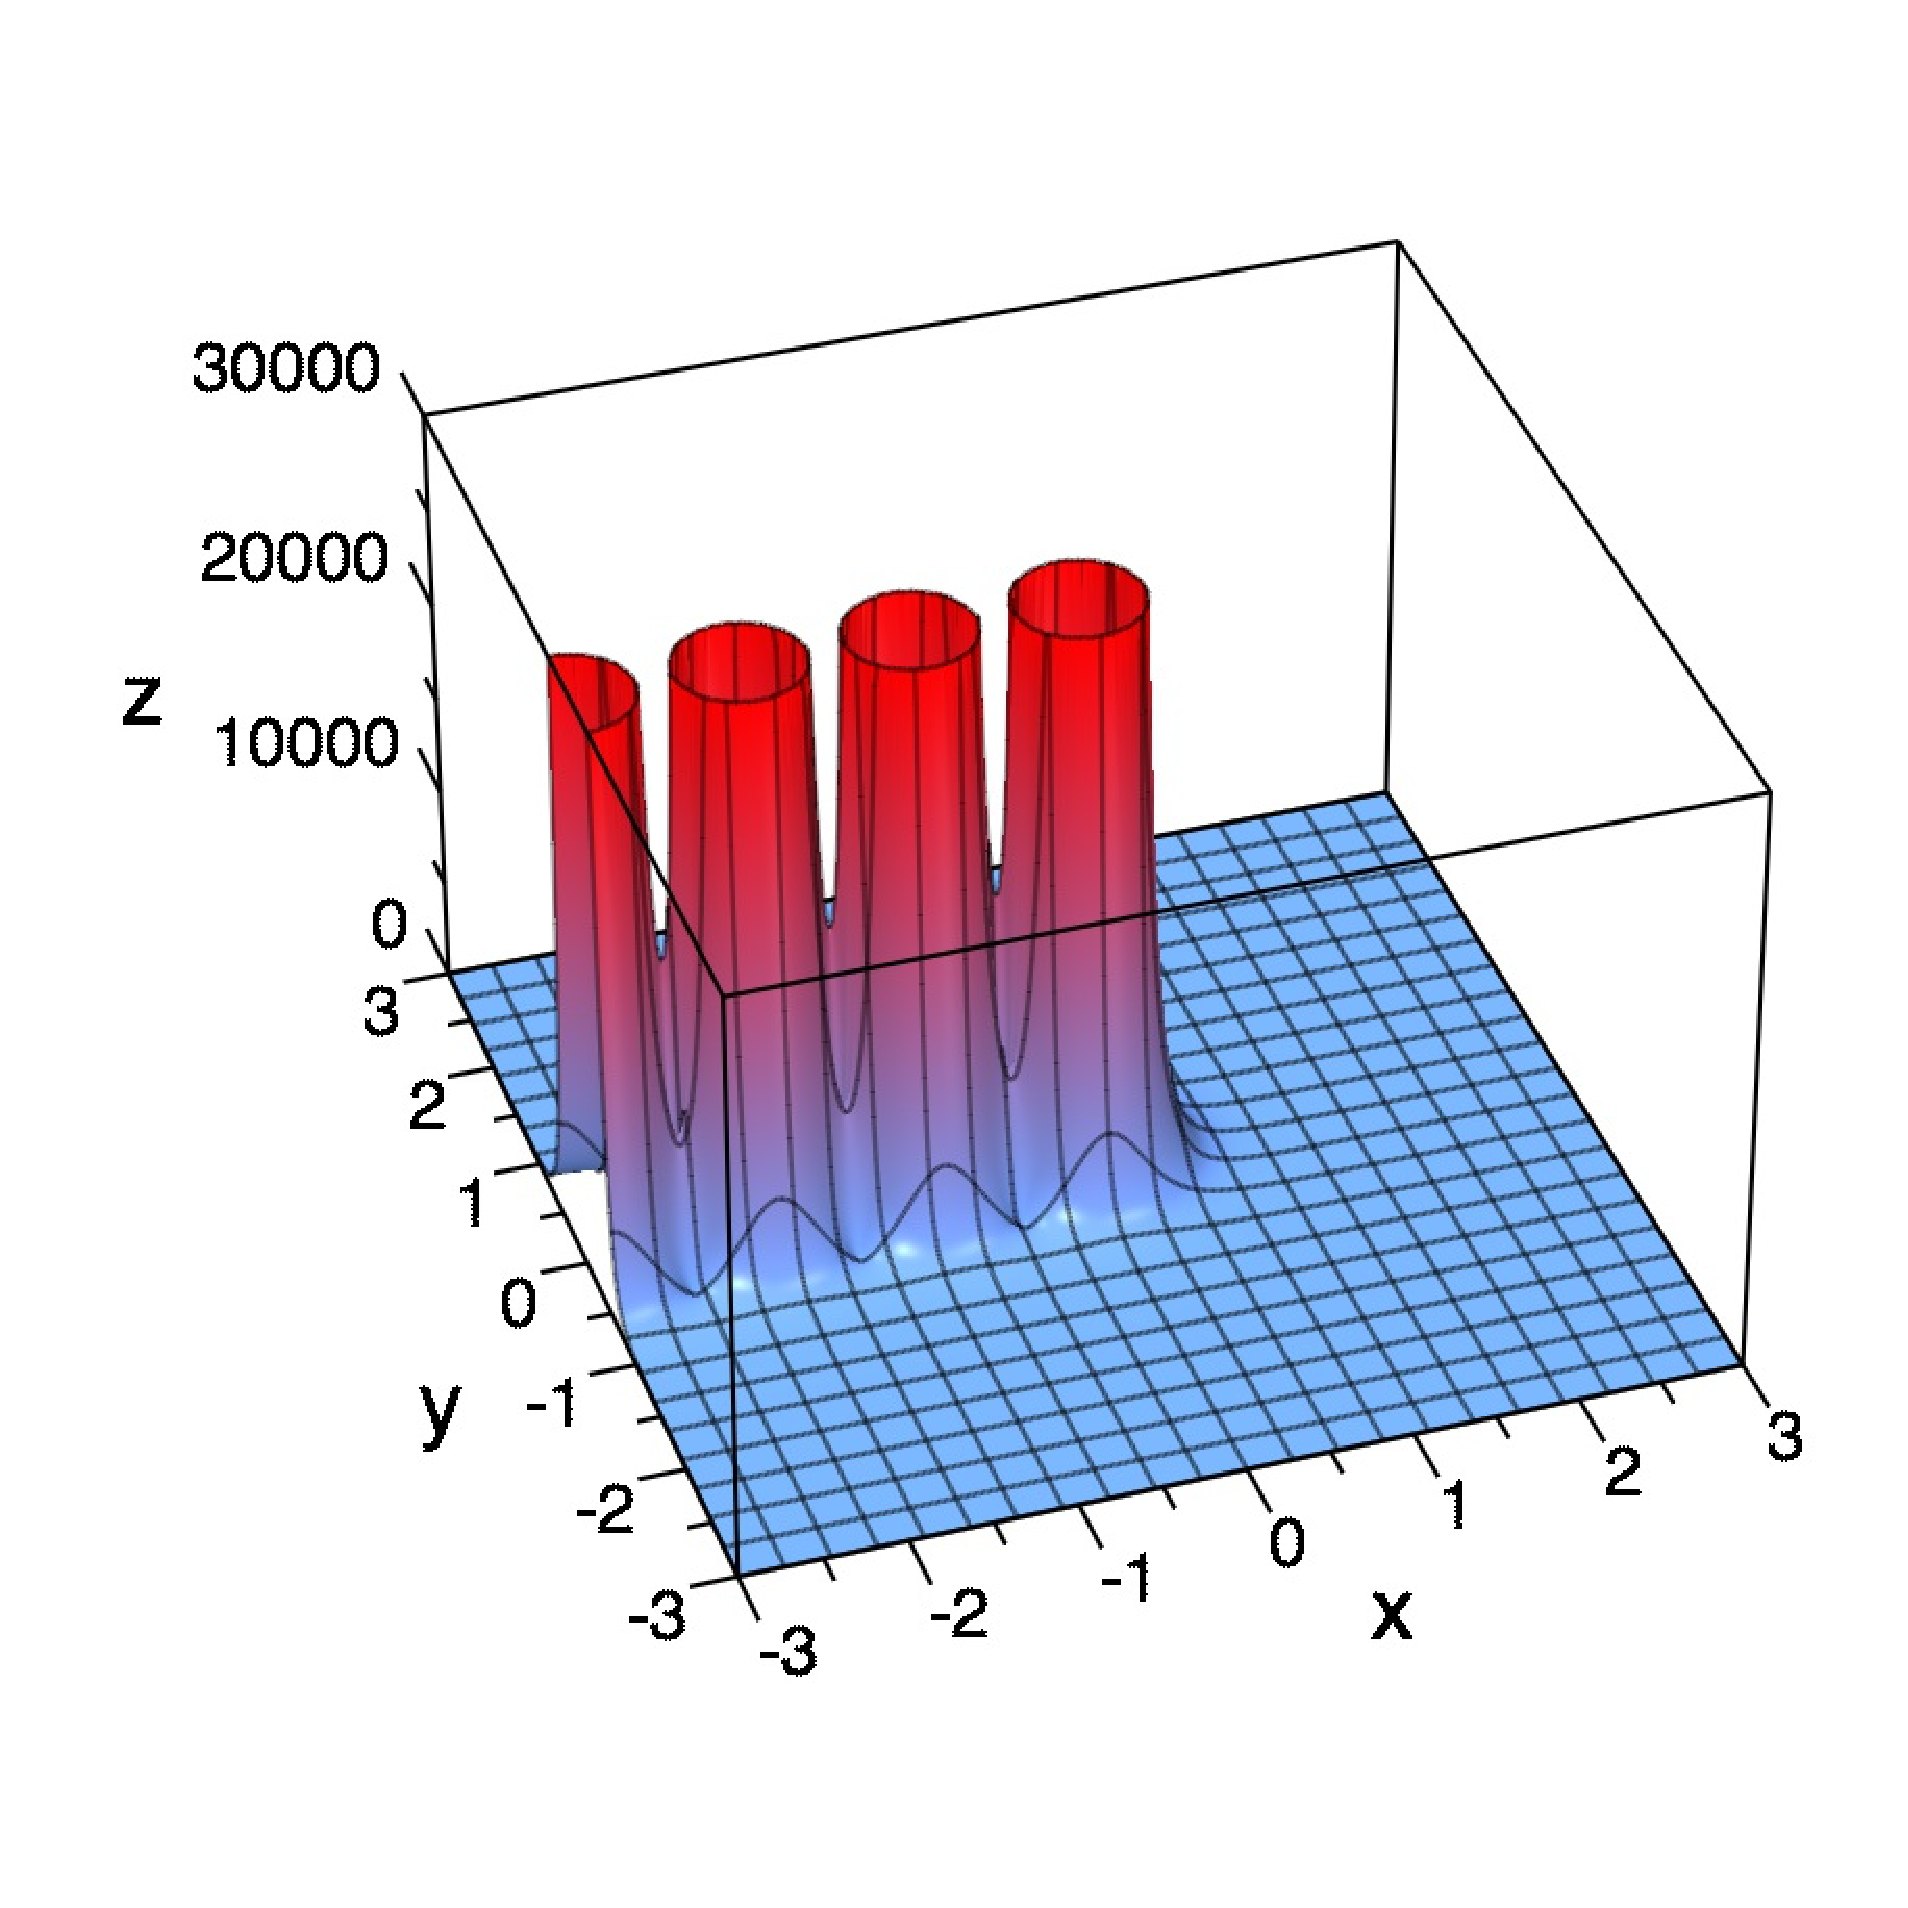
\includegraphics[width = 0.45\textwidth]{Psi5FuncAbs.eps}
        }
    }
    \caption{Polygamma 함수의 그래프.}
\end{figure}

앞서 보인 것과 같이 감마함수가 $\mathcal{C}^\infty$급 함수이므로 $\log\Gamma(x)$도 $\mathcal{C}^\infty$급이 되어 프사이함수와 polygamma 함수는 well-define된다. 이제 프사이함수와 trigamma 함수의 성질들을 간단히 살펴보자. 첫째로 살펴볼 성질은 정의로부터 거의 자명하고, 그 다음 성질은 조금 덜 자명하다.

\begin{proposition}
    임의의 $x>0$에 대해 다음이 성립한다.
    \begin{enumerate}
        \item $\psi(x)=\Gamma'(x)/\Gamma(x)$.
        \item $\psi_1(x)=\Gamma''(x)/\Gamma(x)-[\psi(x)]^2$.
    \end{enumerate}
\end{proposition}

\begin{proof}
    이는 정의로부터 거의 자명하다. i의 경우 $\psi(x)=d(\log\Gamma(x))/dx=\Gamma'(x)/\Gamma(x)$이고, ii의 경우 i로부터 $\psi_1(x)=\psi'(x)=\{\Gamma''(x)\Gamma(x)-[\Gamma'(x)]^2\}/[\Gamma(x)]^2=\Gamma''(x)/\Gamma(x)-[\psi(x)]^2$이다.
\end{proof}

\begin{theorem}
    임의의 $x>0$에 대해 다음이 성립한다.
    \begin{enumerate}
        \item $\psi(x)=-\gamma-1/x+\sum_{k=1}^\infty x/k(k+x)$.
        \item $\psi_1(x)=\sum_{k=0}^\infty1/(k+x)^2$.
    \end{enumerate}
\end{theorem}

\begin{proof}
    증명에 앞서 임의의 $x_0>0$를 고정하자.

    i. 감마함수의 Weierstrass의 무한곱 표현을 생각하면 임의의 $x>0$에 대해 $\log\Gamma(x)=-\gamma x-\log x+\sum_{k=1}^\infty[x/k-\log(1+x/k)]$인데, 여기서 급수의 각 항이 미분가능하고 각 항의 도함수로 이루어진 급수 $\sum_{k=1}^\infty x/k(k+x)$가 $x_0$의 근방에서 균등수렴하므로\footnote{
        점 $x_0$의 근방의 $x>0$에 대해 적당한 $M>0$이 존재하여 $|x|\leq M$이므로 임의의 $k\in\mathbb{N}$에 대해 $x/k(k+x)\leq M/k^2$이고, $\sum_{k=1}^\infty M/k^2=M\pi^2/6<\infty$이므로 Weierstrass의 M-판정법으로부터 $\sum_{k=1}^\infty x/k(k+x)$가 $x_0$의 근방에서 균등수렴한다.
    } 위 식의 양변을 $x_0$에서 미분하면 $\psi(x_0)=-\gamma-1/x_0+\sum_{k=1}^\infty x/k(k+x_0)$를 얻는다.

    ii. i에서 급수의 각 항이 미분가능하고 각 항의 도함수로 이루어진 급수 $\sum_{k=1}^\infty1/(k+x)^2$가 $x_0$의 근방에서 균등수렴하므로\footnote{
        이 급수는 사실 $\mathbb{R}^+$ 전체에서 균등수렴한다. 임의의 $x>0$와 임의의 $k\in\mathbb{N}$에 대해 $1/(k+x)^2\leq1/k^2$이고, $\sum_{k=1}^\infty 1/k^2=\pi^2/6<\infty$이므로 Weierstrass의 M-판정법으로부터 $\sum_{k=1}^\infty1/(k+x)^2$은 $\mathbb{R}^+$에서 균등수렴한다.
    } i의 양변을 $x_0$에서 미분하면 $\psi_1(x_0)=1/x^2+\sum_{k=1}^\infty1/(k+x)^2=\sum_{k=0}^\infty1/(k+x)^2$을 얻는다.
\end{proof}

감마함수의 성질로부터 비롯되는 polygamma 함수의 성질 하나를 증명하는 것을 끝으로 프사이함수와 polygamma 함수에 대한 내용은 마무리하도록 하자.

\begin{theorem}
    임의의 $n\in\mathbb{N}_0$과 임의의 $x>0$에 대해 $\psi_n(x+1)=\psi_n(x)+(-1)^nn!/x^{n+1}$이다.
\end{theorem}

\begin{proof}
    먼저 $n=0$인 경우, 감마함수의 성질로부터 임의의 $x>0$에 대해 $\log\Gamma(x+1)=\log\Gamma(x)+\log x$가 성립하므로 양변을 미분하면 곧바로 $\psi(x+1)=\psi(x)+1/x$를 얻는다. 이제 이의 양변을 $n$번 미분하면 원하는 결과를 얻을 수 있다.
\end{proof}

\subsection{Beta Function}

이번에 알아볼 함수는 감마함수의 비로 정의되는 함수이다.

\begin{definition}
    다음과 같이 정의되는 함수 $\Be:(\mathbb{R}^+)^2\to\mathbb{R}^+$를 \textbf{베타함수(beta function)}라 한다.
    \begin{equation*}
        \Be:(x,\,y)\mapsto\int_0^1t^{x-1}(1-t)^{y-1}\,dt
    \end{equation*}
\end{definition}

역시 이번에도 베타함수가 well-define되는지 살펴보아야 하는데, 이는 다음 명제를 보이는 것으로 충분하다.

\begin{proposition}\label{prop:betaWellDefine}
    임의의 $\alpha,\,\beta\in\mathbb{R}$에 대해 $I(\alpha,\,\beta)=\int_0^1x^{\alpha-1}(1-x)^{\beta-1}\,dx$라 하면 $\alpha,\,\beta>0$일때 $I(\alpha,\,\beta)<\infty$이고 그렇지 않으면 $I(\alpha,\,\beta)=\infty$이다.
\end{proposition}

\begin{proof}
    먼저 $\alpha\leq0$인 경우를 생각하면 충분히 큰 $n\in\mathbb{N}$에 대해
    \begin{align*}
        I(\alpha,\,\beta)&\geq\int_0^1\frac{(1-x)^\beta}{x}\,dx\\
        &\geq\int_0^1\frac{(1-x)^n}{x}\,dx\\
        &=\int_0^1\sum_{k=0}^n\binom{n}{k}(-1)^kx^{k-1}\,dx\\
        &=\sum_{k=1}^n\binom{n}{k}(-1)^k\int_0^1x^{k-1}\,dx+\int_0^1\frac{1}{x}\,dx\\
        &=\sum_{k=1}^n\binom{n}{k}\frac{(-1)^k}{k}+[\log x]_0^1\\
        &=\infty
    \end{align*}
    이고, $\beta\leq0$인 경우에도 비슷하게 같은 결론을 얻는다. 한편, $\alpha,\,\beta>0$이면 간단한 치환적분으로부터
    \begin{align*}
        \Gamma(\alpha)\Gamma(\beta)&=\int_0^\infty t^{\alpha-1}(1-t)^{\beta-1}\,dx\int_0^\infty s^{\alpha-1}e^{-s}\,ds\\
        &=\int_{(\mathbb{R}^+)^2}t^{\alpha-1}s^{\beta-1}e^{-(t+s)}\,dt\,ds\\
        &=\int_0^1\int_0^\infty(uv)^{\alpha-1}[u(1-v)]^{\beta-1}e^{-u}u\,du\,dv&\because(t,\,s)=(uv,\,u(1-v))\\
        &=\bigg[\int_0^\infty u^{\alpha+\beta-1}e^{-u}\,du\bigg]\bigg[\int_0^1v^{\alpha-1}(1-v)^{\beta-1}\,dv\bigg]\\
        &=\Gamma(\alpha+\beta)I(\alpha,\,\beta)
    \end{align*}
    가 성립하고, 곧 $I(\alpha,\,\beta)=\Gamma(\alpha)\Gamma(\beta)/\Gamma(\alpha+\beta)<\infty$이다.
\end{proof}

\begin{figure}[!ht]
    \centering
    \subfigure{
        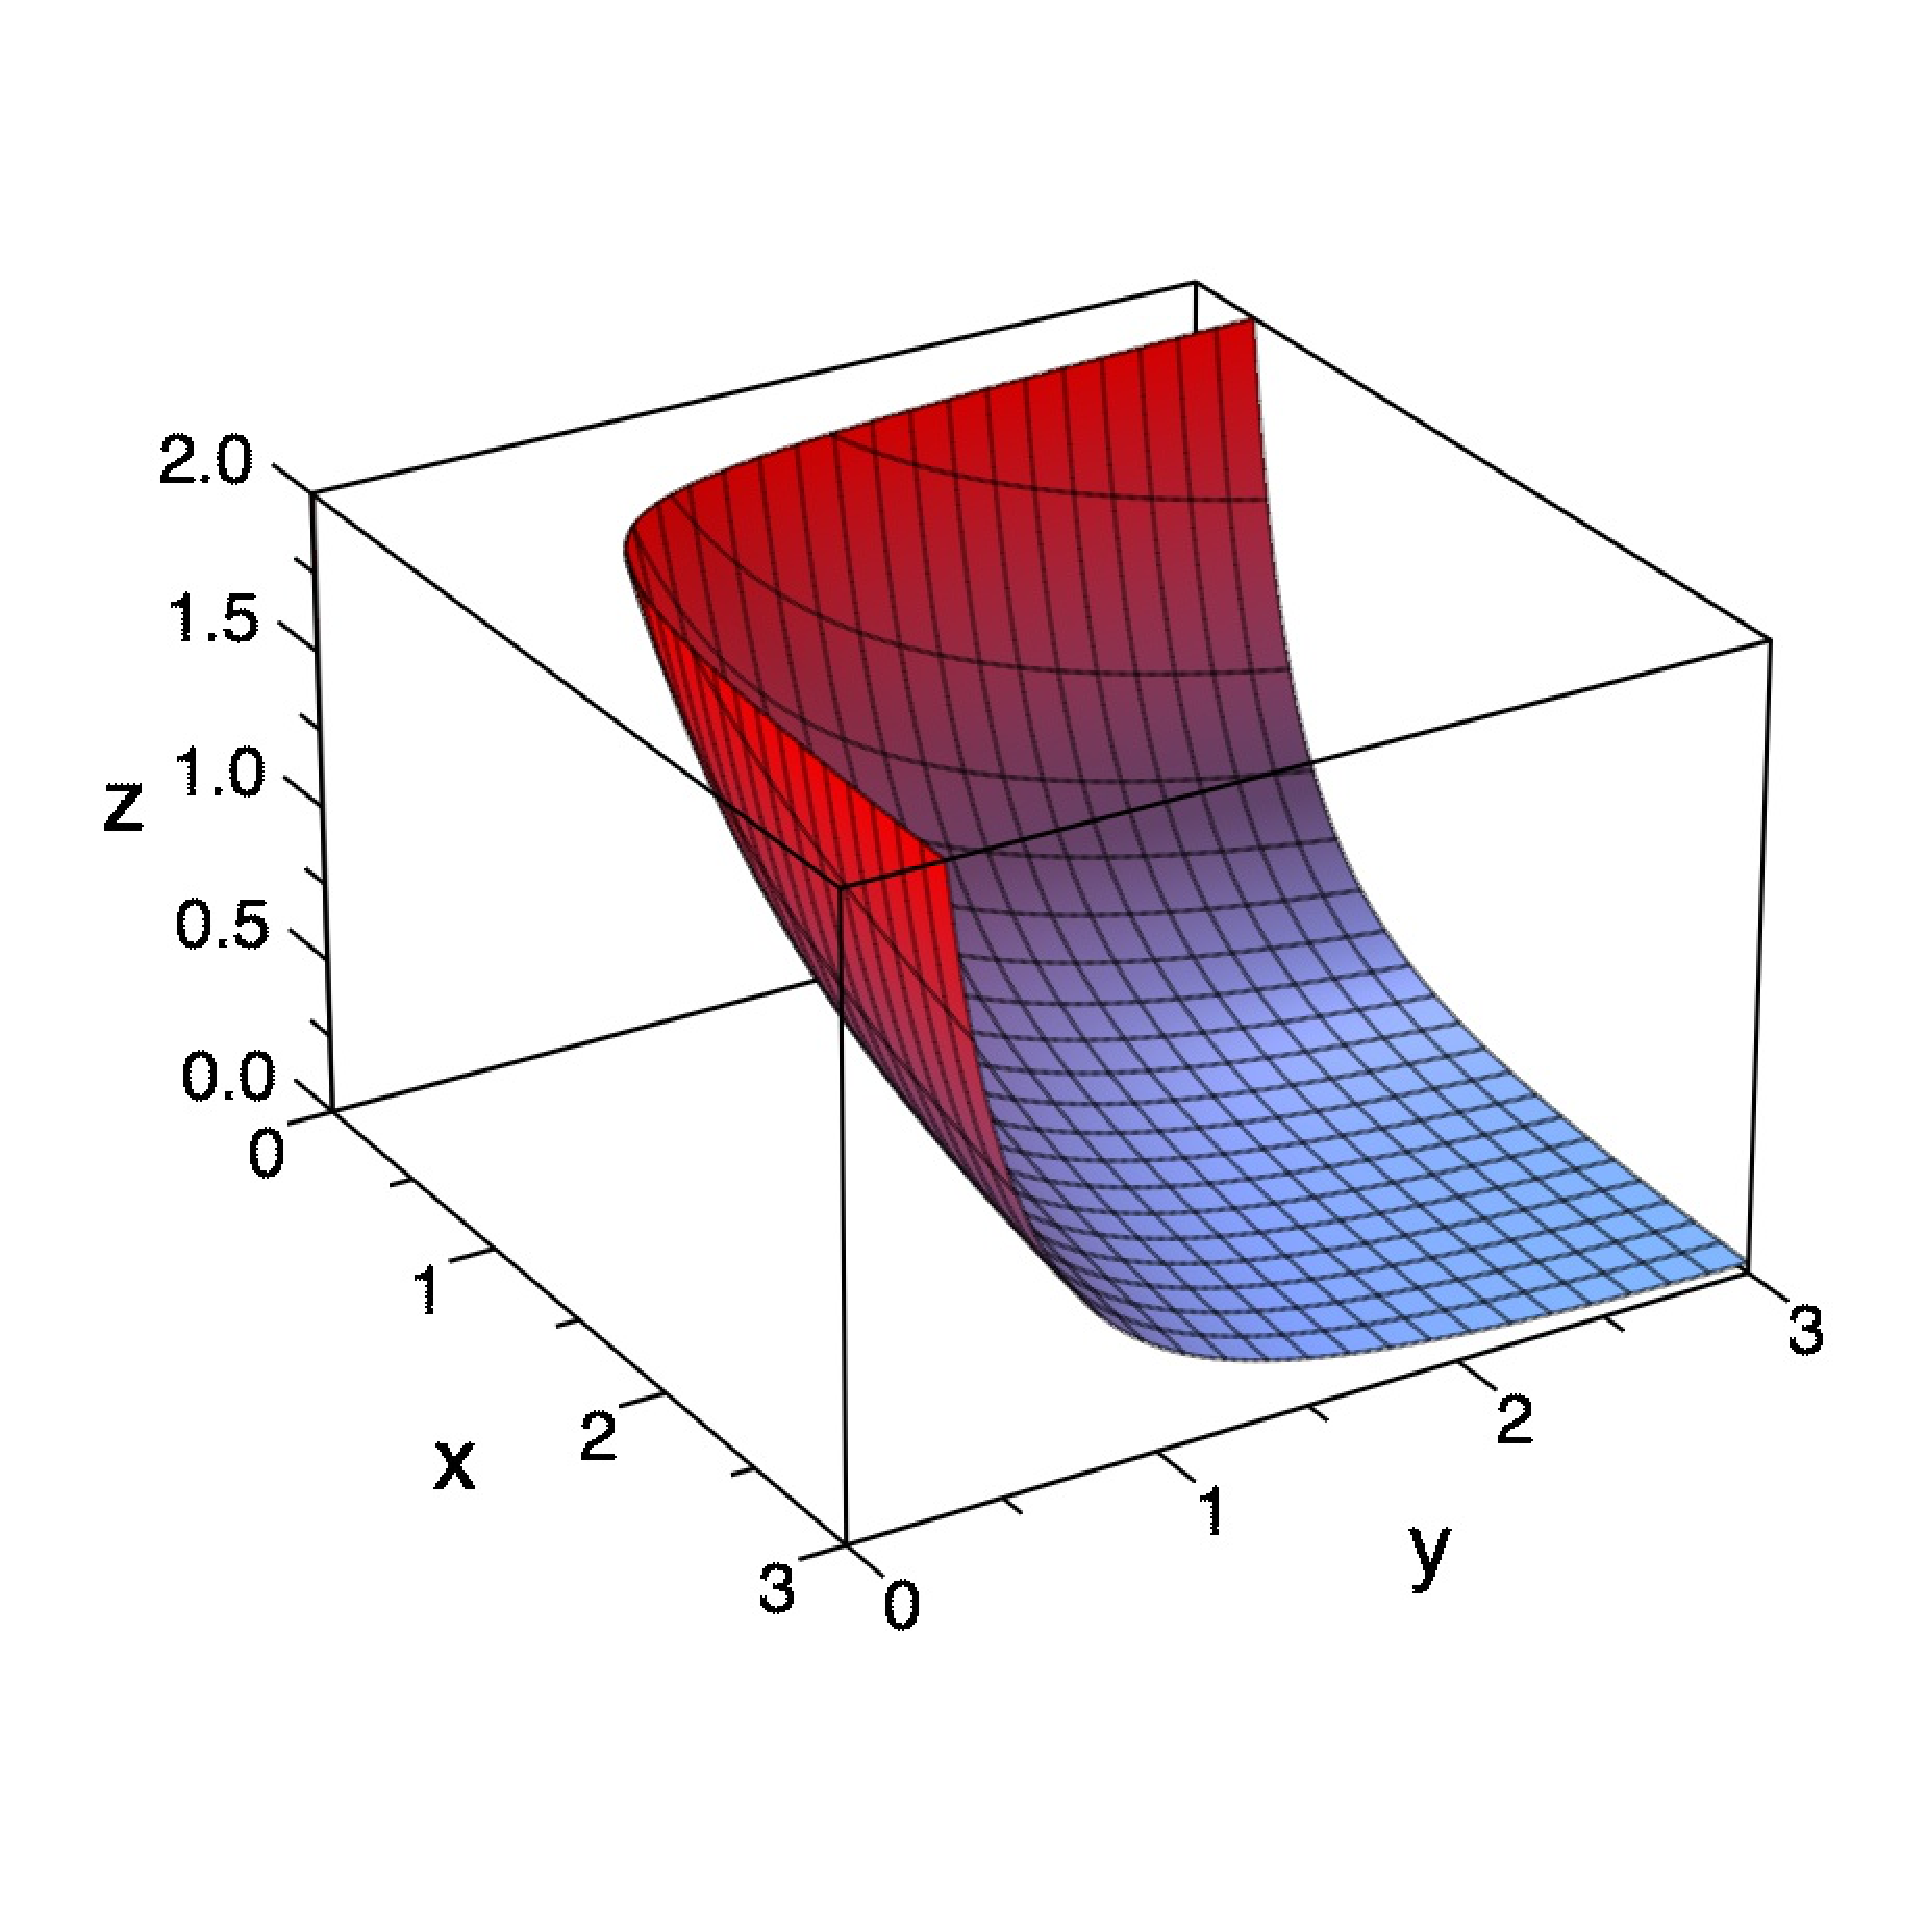
\includegraphics[width = 0.45\textwidth]{BetaFunc.eps}
    }
    \subfigure{
        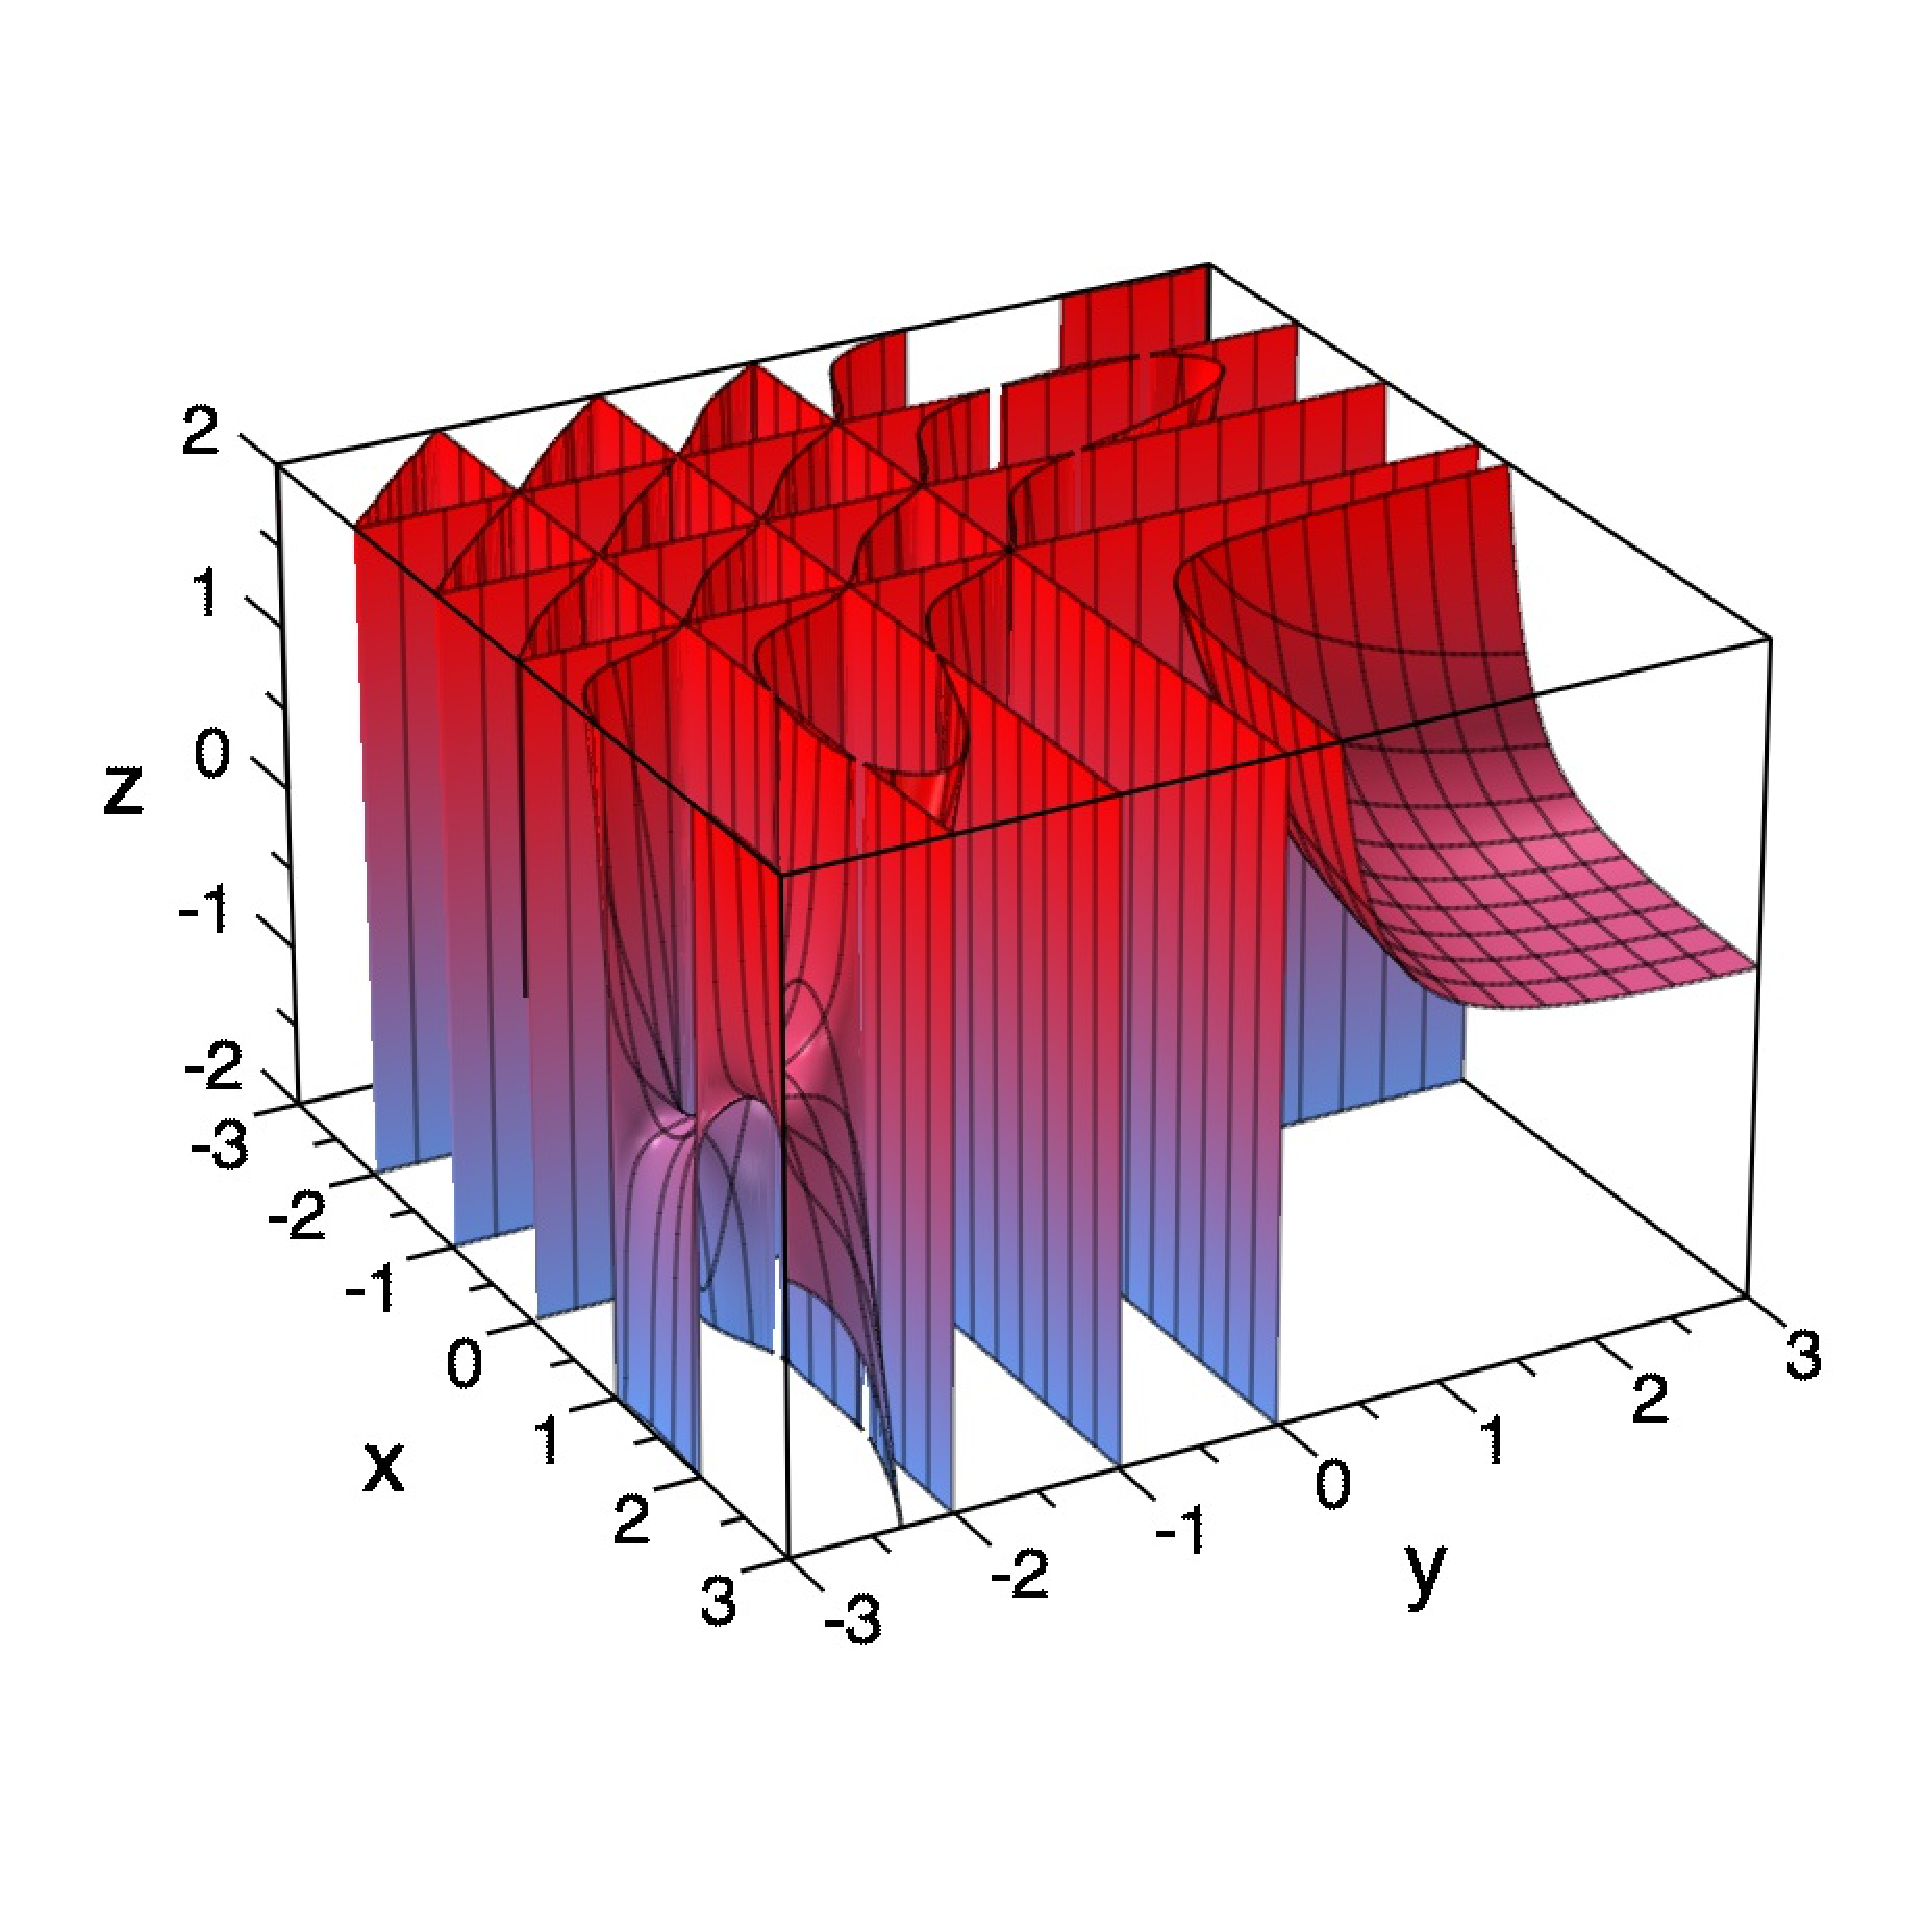
\includegraphics[width = 0.45\textwidth]{BetaFuncExpand.eps}
    }
    \caption{베타함수 $z=\Be(x,\,y)$의 그래프. (왼쪽) 한편, 베타함수도 그 정의역을 $\mathbb{C}$로 자연스럽게 확장할 수 있는데, 참고삼아 $[-3,\,3]^2$에서의 $z=\Be(x,\,y)$의 그래프를 실었다. 당연히 본문에는 이와 관련된 내용이 없었으므로, 이 책에서 이런 사실이 사용되지는 않을 것이다. (Rendered by MATLAB Symbolic Math Toolbox MuPAD.)}
\end{figure}

그리고 이러한 베타함수로부터 파생되는 불완전 베타함수들도 있는데, 이번에도 그냥 이름과 정의 정도만 익혀두면 된다.

\begin{definition}
    임의의 $\alpha,\,\beta>0$에 대해 다음과 같이 정의되는 함수 $\Be(\cdot;\alpha,\,\beta):[0,\,1]\to\mathbb{R}^+_0$를 \textbf{불완전 베타함수(incomplete beta function)}라 한다.
    \begin{equation*}
        \Be(\cdot;\alpha,\,\beta):x\mapsto\int_0^xt^{\alpha-1}(1-t)^{\beta-1}\,dt
    \end{equation*}
    나아가, 다음과 같이 정의되는 함수 $I_x(\alpha,\,\beta):[0,\,1]\to\mathbb{R}^+_0$를 \textbf{정규화된 불완전 베타함수(regularized incomplete beta function)}라 한다.
    \begin{equation*}
        I_x(\alpha,\,\beta)=\frac{\Be(x;\alpha,\,\beta)}{\Be(\alpha,\,\beta)}
    \end{equation*}
\end{definition}

\begin{figure}[!ht]
    \centering
    \subfigure{
        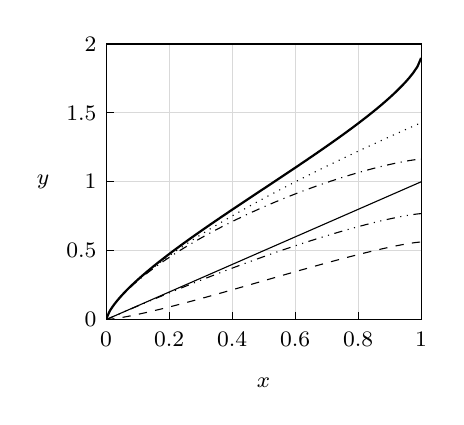
\begin{tikzpicture}
            \begin{scope}[every node/.append style = {font = \footnotesize}]
                \foreach \x in {0, 0.2, 0.4, 0.6, 0.8, 1}
                    \node at (4*\x,-0.25) {$\x$};
                \foreach \x in {0.2, 0.4, 0.6, 0.8} {
                    \draw[style = thin, gray!30!white] (4*\x,0) -- (4*\x,3.5);
                    \draw (4*\x,0) -- (4*\x,0.1);
                }
                \foreach \y in {0, 0.5, ..., 2}
                    \node[anchor = east] at (0,3.5*\y/2) {$\y$};
                \foreach \y in {0.5, 1, 1.5} {
                    \draw[style = thin, gray!30!white] (0,3.5*\y/2) -- (4,3.5*\y/2);
                    \draw (0,3.5*\y/2) -- (0.1,3.5*\y/2);
                }
                \node at (2,-0.8) {$x$};
                \node at (-0.8,1.75) {$y$};
            \end{scope}
            \begin{scope}
            \draw[clip] (0,0) -- (4,0) -- (4,3.5) -- (0,3.5) -- cycle;
            \draw[style = thick] plot[smooth, tension = 0.7] coordinates{(0.,0.) (0.05,0.116533) (0.1,0.189606) (0.15,0.252232) (0.2,0.308993) (0.25,0.361813) (0.3,0.411733) (0.35,0.459398) (0.4,0.505245) (0.45,0.549583) (0.5,0.592646) (0.55,0.634613) (0.6,0.675627) (0.65,0.715805) (0.7,0.755241) (0.75,0.794016) (0.8,0.832198) (0.85,0.869847) (0.9,0.907013) (0.95,0.943742) (1.,0.980073) (1.05,1.01604) (1.1,1.05168) (1.15,1.08702) (1.2,1.12209) (1.25,1.1569) (1.3,1.19149) (1.35,1.22587) (1.4,1.26007) (1.45,1.2941) (1.5,1.32797) (1.55,1.36171) (1.6,1.39533) (1.65,1.42884) (1.7,1.46227) (1.75,1.49562) (1.8,1.5289) (1.85,1.56213) (1.9,1.59533) (1.95,1.6285) (2.,1.66166) (2.05,1.69482) (2.1,1.72799) (2.15,1.76118) (2.2,1.79442) (2.25,1.8277) (2.3,1.86105) (2.35,1.89447) (2.4,1.92799) (2.45,1.96161) (2.5,1.99535) (2.55,2.02922) (2.6,2.06325) (2.65,2.09744) (2.7,2.13182) (2.75,2.16641) (2.8,2.20123) (2.85,2.23629) (2.9,2.27163) (2.95,2.30727) (3.,2.34324) (3.05,2.37957) (3.1,2.4163) (3.15,2.45347) (3.2,2.49112) (3.25,2.5293) (3.3,2.56808) (3.35,2.60751) (3.4,2.64769) (3.45,2.6887) (3.5,2.73067) (3.55,2.77373) (3.6,2.81807) (3.65,2.86392) (3.7,2.91158) (3.75,2.9615) (3.8,3.01432) (3.85,3.07108) (3.9,3.13371) (3.95,3.20678) (4.,3.32332)};
            \draw plot[smooth, tension = 0.7] coordinates{(0.,0.) (0.05,0.021875) (0.1,0.04375) (0.15,0.065625) (0.2,0.0875) (0.25,0.109375) (0.3,0.13125) (0.35,0.153125) (0.4,0.175) (0.45,0.196875) (0.5,0.21875) (0.55,0.240625) (0.6,0.2625) (0.65,0.284375) (0.7,0.30625) (0.75,0.328125) (0.8,0.35) (0.85,0.371875) (0.9,0.39375) (0.95,0.415625) (1.,0.4375) (1.05,0.459375) (1.1,0.48125) (1.15,0.503125) (1.2,0.525) (1.25,0.546875) (1.3,0.56875) (1.35,0.590625) (1.4,0.6125) (1.45,0.634375) (1.5,0.65625) (1.55,0.678125) (1.6,0.7) (1.65,0.721875) (1.7,0.74375) (1.75,0.765625) (1.8,0.7875) (1.85,0.809375) (1.9,0.83125) (1.95,0.853125) (2.,0.875) (2.05,0.896875) (2.1,0.91875) (2.15,0.940625) (2.2,0.9625) (2.25,0.984375) (2.3,1.00625) (2.35,1.02813) (2.4,1.05) (2.45,1.07188) (2.5,1.09375) (2.55,1.11563) (2.6,1.1375) (2.65,1.15938) (2.7,1.18125) (2.75,1.20313) (2.8,1.225) (2.85,1.24688) (2.9,1.26875) (2.95,1.29063) (3.,1.3125) (3.05,1.33438) (3.1,1.35625) (3.15,1.37813) (3.2,1.4) (3.25,1.42188) (3.3,1.44375) (3.35,1.46563) (3.4,1.4875) (3.45,1.50938) (3.5,1.53125) (3.55,1.55313) (3.6,1.575) (3.65,1.59688) (3.7,1.61875) (3.75,1.64063) (3.8,1.6625) (3.85,1.68438) (3.9,1.70625) (3.95,1.72813) (4.,1.75)};
            \draw[style = dashed] plot[smooth, tension = 0.7] coordinates{(0.,0.) (0.05,0.00450976) (0.1,0.0110805) (0.15,0.0187301) (0.2,0.0271651) (0.25,0.0362275) (0.3,0.0458152) (0.35,0.0558558) (0.4,0.0662943) (0.45,0.0770876) (0.5,0.0882003) (0.55,0.099603) (0.6,0.11127) (0.65,0.123181) (0.7,0.135315) (0.75,0.147656) (0.8,0.160189) (0.85,0.172899) (0.9,0.185774) (0.95,0.198803) (1.,0.211974) (1.05,0.225277) (1.1,0.238704) (1.15,0.252244) (1.2,0.265891) (1.25,0.279635) (1.3,0.293469) (1.35,0.307387) (1.4,0.321381) (1.45,0.335444) (1.5,0.34957) (1.55,0.363753) (1.6,0.377986) (1.65,0.392264) (1.7,0.40658) (1.75,0.420929) (1.8,0.435306) (1.85,0.449705) (1.9,0.46412) (1.95,0.478546) (2.,0.492977) (2.05,0.507408) (2.1,0.521834) (2.15,0.536249) (2.2,0.550648) (2.25,0.565024) (2.3,0.579374) (2.35,0.59369) (2.4,0.607968) (2.45,0.622201) (2.5,0.636384) (2.55,0.65051) (2.6,0.664573) (2.65,0.678567) (2.7,0.692484) (2.75,0.706319) (2.8,0.720063) (2.85,0.73371) (2.9,0.74725) (2.95,0.760677) (3.,0.77398) (3.05,0.787151) (3.1,0.80018) (3.15,0.813055) (3.2,0.825765) (3.25,0.838298) (3.3,0.850639) (3.35,0.862773) (3.4,0.874683) (3.45,0.886351) (3.5,0.897754) (3.55,0.908866) (3.6,0.91966) (3.65,0.930098) (3.7,0.940139) (3.75,0.949726) (3.8,0.958789) (3.85,0.967224) (3.9,0.974873) (3.95,0.981444) (4.,0.985954)};
            \draw[style = dotted] plot[smooth, tension = 0.7] coordinates{(0.,0.) (0.05,0.116353) (0.1,0.189016) (0.15,0.251051) (0.2,0.307057) (0.25,0.358968) (0.3,0.407833) (0.35,0.454303) (0.4,0.498816) (0.45,0.541685) (0.5,0.583146) (0.55,0.623379) (0.6,0.662527) (0.65,0.700708) (0.7,0.738017) (0.75,0.774535) (0.8,0.810328) (0.85,0.845456) (0.9,0.87997) (0.95,0.913912) (1.,0.947323) (1.05,0.980236) (1.1,1.01268) (1.15,1.04469) (1.2,1.07628) (1.25,1.10748) (1.3,1.1383) (1.35,1.16878) (1.4,1.19891) (1.45,1.22873) (1.5,1.25824) (1.55,1.28745) (1.6,1.31638) (1.65,1.34504) (1.7,1.37345) (1.75,1.4016) (1.8,1.42952) (1.85,1.4572) (1.9,1.48465) (1.95,1.5119) (2.,1.53893) (2.05,1.56576) (2.1,1.5924) (2.15,1.61884) (2.2,1.64511) (2.25,1.67119) (2.3,1.6971) (2.35,1.72284) (2.4,1.74842) (2.45,1.77384) (2.5,1.7991) (2.55,1.82422) (2.6,1.84918) (2.65,1.874) (2.7,1.89868) (2.75,1.92323) (2.8,1.94764) (2.85,1.97192) (2.9,1.99607) (2.95,2.0201) (3.,2.04401) (3.05,2.0678) (3.1,2.09147) (3.15,2.11502) (3.2,2.13847) (3.25,2.1618) (3.3,2.18503) (3.35,2.20815) (3.4,2.23117) (3.45,2.25409) (3.5,2.27691) (3.55,2.29963) (3.6,2.32225) (3.65,2.34478) (3.7,2.36722) (3.75,2.38957) (3.8,2.41183) (3.85,2.434) (3.9,2.45608) (3.95,2.47808) (4.,2.5)};
            \draw[style = dashdotted] plot[smooth, tension = 0.7] coordinates{(0.,0.) (0.05,0.116173) (0.1,0.188429) (0.15,0.249878) (0.2,0.305139) (0.25,0.356158) (0.3,0.403991) (0.35,0.449294) (0.4,0.492512) (0.45,0.533961) (0.5,0.573879) (0.55,0.61245) (0.6,0.649818) (0.65,0.686102) (0.7,0.721399) (0.75,0.75579) (0.8,0.789344) (0.85,0.822121) (0.9,0.854171) (0.95,0.885538) (1.,0.916263) (1.05,0.946379) (1.1,0.975917) (1.15,1.0049) (1.2,1.03337) (1.25,1.06132) (1.3,1.0888) (1.35,1.1158) (1.4,1.14236) (1.45,1.16849) (1.5,1.19419) (1.55,1.21949) (1.6,1.24439) (1.65,1.2689) (1.7,1.29304) (1.75,1.31681) (1.8,1.34021) (1.85,1.36327) (1.9,1.38598) (1.95,1.40836) (2.,1.4304) (2.05,1.45211) (2.1,1.4735) (2.15,1.49457) (2.2,1.51532) (2.25,1.53576) (2.3,1.55589) (2.35,1.57572) (2.4,1.59524) (2.45,1.61446) (2.5,1.63338) (2.55,1.65199) (2.6,1.67031) (2.65,1.68833) (2.7,1.70605) (2.75,1.72346) (2.8,1.74058) (2.85,1.75739) (2.9,1.7739) (2.95,1.7901) (3.,1.80599) (3.05,1.82157) (3.1,1.83682) (3.15,1.85175) (3.2,1.86635) (3.25,1.88061) (3.3,1.89453) (3.35,1.90809) (3.4,1.92128) (3.45,1.93408) (3.5,1.94649) (3.55,1.95848) (3.6,1.97002) (3.65,1.9811) (3.7,1.99166) (3.75,2.00167) (3.8,2.01105) (3.85,2.01972) (3.9,2.02752) (3.95,2.03416) (4.,2.03869)};
            \draw[style = dashdotdotted] plot[smooth, tension = 0.7] coordinates{(0.,0.) (0.05,0.0218339) (0.1,0.043585) (0.15,0.0652526) (0.2,0.0868359) (0.25,0.108334) (0.3,0.129747) (0.35,0.151073) (0.4,0.172311) (0.45,0.193461) (0.5,0.214522) (0.55,0.235493) (0.6,0.256373) (0.65,0.277161) (0.7,0.297856) (0.75,0.318457) (0.8,0.338963) (0.85,0.359374) (0.9,0.379687) (0.95,0.399903) (1.,0.420019) (1.05,0.440035) (1.1,0.459949) (1.15,0.479761) (1.2,0.499468) (1.25,0.519071) (1.3,0.538566) (1.35,0.557954) (1.4,0.577232) (1.45,0.5964) (1.5,0.615454) (1.55,0.634395) (1.6,0.653221) (1.65,0.671929) (1.7,0.690518) (1.75,0.708986) (1.8,0.727331) (1.85,0.745552) (1.9,0.763646) (1.95,0.781611) (2.,0.799446) (2.05,0.817147) (2.1,0.834712) (2.15,0.852139) (2.2,0.869426) (2.25,0.886569) (2.3,0.903565) (2.35,0.920412) (2.4,0.937107) (2.45,0.953646) (2.5,0.970026) (2.55,0.986243) (2.6,1.00229) (2.65,1.01817) (2.7,1.03387) (2.75,1.0494) (2.8,1.06474) (2.85,1.07988) (2.9,1.09483) (2.95,1.10958) (3.,1.12412) (3.05,1.13844) (3.1,1.15254) (3.15,1.16641) (3.2,1.18003) (3.25,1.1934) (3.3,1.2065) (3.35,1.21933) (3.4,1.23186) (3.45,1.24409) (3.5,1.25598) (3.55,1.26752) (3.6,1.27869) (3.65,1.28944) (3.7,1.29974) (3.75,1.30953) (3.8,1.31875) (3.85,1.3273) (3.9,1.33503) (3.95,1.34163) (4.,1.34615)};
            \end{scope}
        \end{tikzpicture}
    }
    \qquad
    \subfigure{
        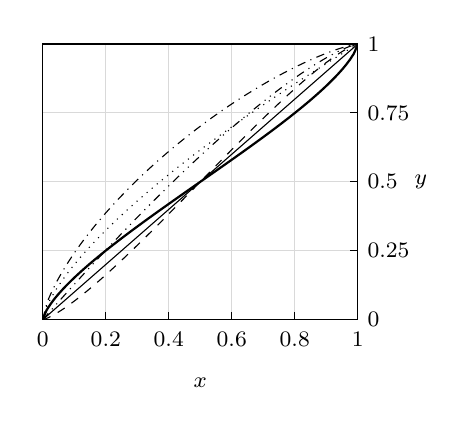
\begin{tikzpicture}
            \begin{scope}[every node/.append style = {font = \footnotesize}]
                \foreach \x in {0, 0.2, 0.4, 0.6, 0.8, 1}
                    \node at (4*\x,-0.25) {$\x$};
                \foreach \x in {0.2, 0.4, 0.6, 0.8} {
                    \draw[style = thin, gray!30!white] (4*\x,0) -- (4*\x,3.5);
                    \draw (4*\x,0) -- (4*\x,0.1);
                }
                \foreach \y in {0, 0.25, ..., 1}
                    \node[anchor = west] at (4,3.5*\y) {$\y$};
                \foreach \y in {0.25, 0.5, 0.75} {
                    \draw[style = thin, gray!30!white] (0,3.5*\y) -- (4,3.5*\y);
                    \draw (4,3.5*\y) -- (3.9,3.5*\y);
                }
                \node at (2,-0.8) {$x$};
                \node at (4.8,1.75) {$y$};
            \end{scope}
            \begin{scope}
            \draw[clip] (0,0) -- (4,0) -- (4,3.5) -- (0,3.5) -- cycle;
            \draw[style = thick] plot[smooth, tension = 0.7] coordinates{(0.,0.) (0.05,0.122729) (0.1,0.199686) (0.15,0.265642) (0.2,0.325421) (0.25,0.381049) (0.3,0.433623) (0.35,0.483822) (0.4,0.532106) (0.45,0.578801) (0.5,0.624154) (0.55,0.668352) (0.6,0.711547) (0.65,0.75386) (0.7,0.795393) (0.75,0.836229) (0.8,0.876442) (0.85,0.916092) (0.9,0.955234) (0.95,0.993916) (1.,1.03218) (1.05,1.07006) (1.1,1.1076) (1.15,1.14481) (1.2,1.18174) (1.25,1.21841) (1.3,1.25484) (1.35,1.29105) (1.4,1.32706) (1.45,1.3629) (1.5,1.39857) (1.55,1.43411) (1.6,1.46951) (1.65,1.50481) (1.7,1.54001) (1.75,1.57513) (1.8,1.61018) (1.85,1.64518) (1.9,1.68014) (1.95,1.71508) (2.,1.75) (2.05,1.78492) (2.1,1.81986) (2.15,1.85482) (2.2,1.88982) (2.25,1.92487) (2.3,1.95999) (2.35,1.99519) (2.4,2.03049) (2.45,2.06589) (2.5,2.10143) (2.55,2.1371) (2.6,2.17294) (2.65,2.20895) (2.7,2.24516) (2.75,2.28159) (2.8,2.31826) (2.85,2.35519) (2.9,2.3924) (2.95,2.42994) (3.,2.46782) (3.05,2.50608) (3.1,2.54477) (3.15,2.58391) (3.2,2.62356) (3.25,2.66377) (3.3,2.70461) (3.35,2.74614) (3.4,2.78845) (3.45,2.83165) (3.5,2.87585) (3.55,2.9212) (3.6,2.96789) (3.65,3.01618) (3.7,3.06638) (3.75,3.11895) (3.8,3.17458) (3.85,3.23436) (3.9,3.30031) (3.95,3.37727) (4.,3.5)};
            \draw plot[smooth, tension = 0.7] coordinates{(0.,0.) (0.05,0.04375) (0.1,0.0875) (0.15,0.13125) (0.2,0.175) (0.25,0.21875) (0.3,0.2625) (0.35,0.30625) (0.4,0.35) (0.45,0.39375) (0.5,0.4375) (0.55,0.48125) (0.6,0.525) (0.65,0.56875) (0.7,0.6125) (0.75,0.65625) (0.8,0.7) (0.85,0.74375) (0.9,0.7875) (0.95,0.83125) (1.,0.875) (1.05,0.91875) (1.1,0.9625) (1.15,1.00625) (1.2,1.05) (1.25,1.09375) (1.3,1.1375) (1.35,1.18125) (1.4,1.225) (1.45,1.26875) (1.5,1.3125) (1.55,1.35625) (1.6,1.4) (1.65,1.44375) (1.7,1.4875) (1.75,1.53125) (1.8,1.575) (1.85,1.61875) (1.9,1.6625) (1.95,1.70625) (2.,1.75) (2.05,1.79375) (2.1,1.8375) (2.15,1.88125) (2.2,1.925) (2.25,1.96875) (2.3,2.0125) (2.35,2.05625) (2.4,2.1) (2.45,2.14375) (2.5,2.1875) (2.55,2.23125) (2.6,2.275) (2.65,2.31875) (2.7,2.3625) (2.75,2.40625) (2.8,2.45) (2.85,2.49375) (2.9,2.5375) (2.95,2.58125) (3.,2.625) (3.05,2.66875) (3.1,2.7125) (3.15,2.75625) (3.2,2.8) (3.25,2.84375) (3.3,2.8875) (3.35,2.93125) (3.4,2.975) (3.45,3.01875) (3.5,3.0625) (3.55,3.10625) (3.6,3.15) (3.65,3.19375) (3.7,3.2375) (3.75,3.28125) (3.8,3.325) (3.85,3.36875) (3.9,3.4125) (3.95,3.45625) (4.,3.5)};
            \draw[style = dashed] plot[smooth, tension = 0.7] coordinates{(0.,0.) (0.05,0.016009) (0.1,0.0393343) (0.15,0.0664891) (0.2,0.0964324) (0.25,0.128603) (0.3,0.162638) (0.35,0.19828) (0.4,0.235336) (0.45,0.27365) (0.5,0.313099) (0.55,0.353577) (0.6,0.394995) (0.65,0.437275) (0.7,0.48035) (0.75,0.52416) (0.8,0.568649) (0.85,0.613768) (0.9,0.659473) (0.95,0.705723) (1.,0.752478) (1.05,0.799703) (1.1,0.847365) (1.15,0.895432) (1.2,0.943875) (1.25,0.992665) (1.3,1.04178) (1.35,1.09118) (1.4,1.14086) (1.45,1.19078) (1.5,1.24092) (1.55,1.29127) (1.6,1.3418) (1.65,1.39248) (1.7,1.4433) (1.75,1.49424) (1.8,1.54528) (1.85,1.59639) (1.9,1.64756) (1.95,1.69877) (2.,1.75) (2.05,1.80123) (2.1,1.85244) (2.15,1.90361) (2.2,1.95472) (2.25,2.00576) (2.3,2.0567) (2.35,2.10752) (2.4,2.1582) (2.45,2.20873) (2.5,2.25908) (2.55,2.30922) (2.6,2.35914) (2.65,2.40882) (2.7,2.45822) (2.75,2.50733) (2.8,2.55613) (2.85,2.60457) (2.9,2.65264) (2.95,2.7003) (3.,2.74752) (3.05,2.79428) (3.1,2.84053) (3.15,2.88623) (3.2,2.93135) (3.25,2.97584) (3.3,3.01965) (3.35,3.06272) (3.4,3.10501) (3.45,3.14642) (3.5,3.1869) (3.55,3.22635) (3.6,3.26466) (3.65,3.30172) (3.7,3.33736) (3.75,3.3714) (3.8,3.40357) (3.85,3.43351) (3.9,3.46067) (3.95,3.48399) (4.,3.5)};
            \draw[style = dotted] plot[smooth, tension = 0.7] coordinates{(0.,0.) (0.05,0.162894) (0.1,0.264622) (0.15,0.351471) (0.2,0.42988) (0.25,0.502556) (0.3,0.570967) (0.35,0.636024) (0.4,0.698342) (0.45,0.758359) (0.5,0.816404) (0.55,0.87273) (0.6,0.927538) (0.65,0.980992) (0.7,1.03322) (0.75,1.08435) (0.8,1.13446) (0.85,1.18364) (0.9,1.23196) (0.95,1.27948) (1.,1.32625) (1.05,1.37233) (1.1,1.41775) (1.15,1.46256) (1.2,1.50679) (1.25,1.55047) (1.3,1.59363) (1.35,1.63629) (1.4,1.67848) (1.45,1.72022) (1.5,1.76153) (1.55,1.80243) (1.6,1.84294) (1.65,1.88306) (1.7,1.92283) (1.75,1.96224) (1.8,2.00132) (1.85,2.04008) (1.9,2.07852) (1.95,2.11666) (2.,2.1545) (2.05,2.19207) (2.1,2.22936) (2.15,2.26638) (2.2,2.30315) (2.25,2.33967) (2.3,2.37594) (2.35,2.41198) (2.4,2.44779) (2.45,2.48338) (2.5,2.51874) (2.55,2.5539) (2.6,2.58885) (2.65,2.6236) (2.7,2.65816) (2.75,2.69252) (2.8,2.7267) (2.85,2.76069) (2.9,2.7945) (2.95,2.82814) (3.,2.86161) (3.05,2.89492) (3.1,2.92806) (3.15,2.96103) (3.2,2.99386) (3.25,3.02653) (3.3,3.05904) (3.35,3.09142) (3.4,3.12364) (3.45,3.15573) (3.5,3.18767) (3.55,3.21948) (3.6,3.25116) (3.65,3.2827) (3.7,3.31411) (3.75,3.3454) (3.8,3.37656) (3.85,3.4076) (3.9,3.43852) (3.95,3.46932) (4.,3.5)};
            \draw[style = dashdotted] plot[smooth, tension = 0.7] coordinates{(0.,0.) (0.05,0.199444) (0.1,0.323492) (0.15,0.428988) (0.2,0.523859) (0.25,0.611447) (0.3,0.693566) (0.35,0.771343) (0.4,0.845538) (0.45,0.916698) (0.5,0.985229) (0.55,1.05145) (0.6,1.1156) (0.65,1.17789) (0.7,1.23849) (0.75,1.29753) (0.8,1.35514) (0.85,1.41141) (0.9,1.46643) (0.95,1.52028) (1.,1.57303) (1.05,1.62473) (1.1,1.67544) (1.15,1.72521) (1.2,1.77407) (1.25,1.82207) (1.3,1.86923) (1.35,1.9156) (1.4,1.96119) (1.45,2.00604) (1.5,2.05017) (1.55,2.0936) (1.6,2.13635) (1.65,2.17843) (1.7,2.21987) (1.75,2.26067) (1.8,2.30086) (1.85,2.34045) (1.9,2.37944) (1.95,2.41785) (2.,2.45569) (2.05,2.49296) (2.1,2.52968) (2.15,2.56585) (2.2,2.60148) (2.25,2.63658) (2.3,2.67114) (2.35,2.70518) (2.4,2.73869) (2.45,2.77168) (2.5,2.80416) (2.55,2.83612) (2.6,2.86757) (2.65,2.8985) (2.7,2.92892) (2.75,2.95882) (2.8,2.98821) (2.85,3.01707) (2.9,3.04541) (2.95,3.07322) (3.,3.1005) (3.05,3.12724) (3.1,3.15343) (3.15,3.17907) (3.2,3.20413) (3.25,3.22862) (3.3,3.2525) (3.35,3.27578) (3.4,3.29842) (3.45,3.32041) (3.5,3.34171) (3.55,3.36229) (3.6,3.38211) (3.65,3.40113) (3.7,3.41926) (3.75,3.43644) (3.8,3.45255) (3.85,3.46743) (3.9,3.48081) (3.95,3.49222) (4.,3.5)};
            \draw[style = dashdotdotted] plot[smooth, tension = 0.7] coordinates{(0.,0.) (0.05,0.056768) (0.1,0.113321) (0.15,0.169657) (0.2,0.225773) (0.25,0.281669) (0.3,0.337342) (0.35,0.392789) (0.4,0.448009) (0.45,0.502999) (0.5,0.557757) (0.55,0.612281) (0.6,0.666569) (0.65,0.720618) (0.7,0.774425) (0.75,0.827988) (0.8,0.881304) (0.85,0.934371) (0.9,0.987186) (0.95,1.03975) (1.,1.09205) (1.05,1.14409) (1.1,1.19587) (1.15,1.24738) (1.2,1.29862) (1.25,1.34958) (1.3,1.40027) (1.35,1.45068) (1.4,1.5008) (1.45,1.55064) (1.5,1.60018) (1.55,1.64943) (1.6,1.69837) (1.65,1.74701) (1.7,1.79535) (1.75,1.84336) (1.8,1.89106) (1.85,1.93844) (1.9,1.98548) (1.95,2.03219) (2.,2.07856) (2.05,2.12458) (2.1,2.17025) (2.15,2.21556) (2.2,2.26051) (2.25,2.30508) (2.3,2.34927) (2.35,2.39307) (2.4,2.43648) (2.45,2.47948) (2.5,2.52207) (2.55,2.56423) (2.6,2.60596) (2.65,2.64725) (2.7,2.68807) (2.75,2.72843) (2.8,2.76831) (2.85,2.8077) (2.9,2.84657) (2.95,2.88491) (3.,2.92272) (3.05,2.95995) (3.1,2.99661) (3.15,3.03266) (3.2,3.06808) (3.25,3.10284) (3.3,3.13691) (3.35,3.17026) (3.4,3.20284) (3.45,3.23462) (3.5,3.26555) (3.55,3.29556) (3.6,3.32458) (3.65,3.35254) (3.7,3.37932) (3.75,3.40478) (3.8,3.42876) (3.85,3.45099) (3.9,3.47107) (3.95,3.48825) (4.,3.5)};
            \end{scope}
        \end{tikzpicture}
    }

    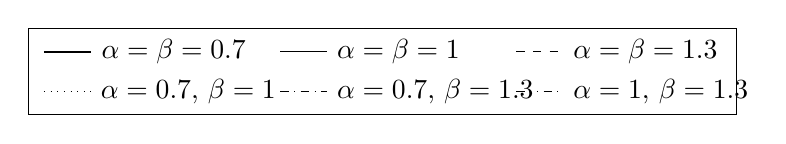
\begin{tikzpicture}
        \draw (0,1.9) -- (9,1.9) -- (9,3) -- (0,3) -- cycle;
        \draw[style = thick] (0.2,2.7) -- (0.8,2.7) node[right] {$\alpha=\beta=0.7$};
        \draw (3.2,2.7) -- (3.8,2.7) node[right] {$\alpha=\beta=1$};
        \draw[style = dashed] (6.2,2.7) -- (6.8,2.7) node[right] {$\alpha=\beta=1.3$};
        \draw[style = dotted] (0.2,2.2) -- (0.8,2.2) node[right] {$\alpha=0.7,\,\beta=1$};
        \draw[style = dashdotted] (3.2,2.2) -- (3.8,2.2) node[right] {$\alpha=0.7,\,\beta=1.3$};
        \draw[style = dashdotdotted] (6.2,2.2) -- (6.8,2.2) node[right] {$\alpha=1,\,\beta=1.3$};
    \end{tikzpicture}
\end{figure}

\begin{figure}[!ht]
    \centering
    \subfigure{
        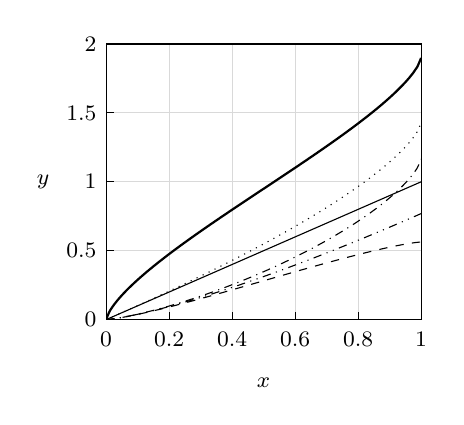
\begin{tikzpicture}
            \begin{scope}[every node/.append style = {font = \footnotesize}]
                \foreach \x in {0, 0.2, 0.4, 0.6, 0.8, 1}
                    \node at (4*\x,-0.25) {$\x$};
                \foreach \x in {0.2, 0.4, 0.6, 0.8} {
                    \draw[style = thin, gray!30!white] (4*\x,0) -- (4*\x,3.5);
                    \draw (4*\x,0) -- (4*\x,0.1);
                }
                \foreach \y in {0, 0.5, ..., 2}
                    \node[anchor = east] at (0,3.5*\y/2) {$\y$};
                \foreach \y in {0.5, 1, 1.5} {
                    \draw[style = thin, gray!30!white] (0,3.5*\y/2) -- (4,3.5*\y/2);
                    \draw (0,3.5*\y/2) -- (0.1,3.5*\y/2);
                }
                \node at (2,-0.8) {$x$};
                \node at (-0.8,1.75) {$y$};
            \end{scope}
            \begin{scope}
            \draw[clip] (0,0) -- (4,0) -- (4,3.5) -- (0,3.5) -- cycle;
            \draw[style = thick] plot[smooth, tension = 0.7] coordinates{(0.,0.) (0.05,0.116533) (0.1,0.189606) (0.15,0.252232) (0.2,0.308993) (0.25,0.361813) (0.3,0.411733) (0.35,0.459398) (0.4,0.505245) (0.45,0.549583) (0.5,0.592646) (0.55,0.634613) (0.6,0.675627) (0.65,0.715805) (0.7,0.755241) (0.75,0.794016) (0.8,0.832198) (0.85,0.869847) (0.9,0.907013) (0.95,0.943742) (1.,0.980073) (1.05,1.01604) (1.1,1.05168) (1.15,1.08702) (1.2,1.12209) (1.25,1.1569) (1.3,1.19149) (1.35,1.22587) (1.4,1.26007) (1.45,1.2941) (1.5,1.32797) (1.55,1.36171) (1.6,1.39533) (1.65,1.42884) (1.7,1.46227) (1.75,1.49562) (1.8,1.5289) (1.85,1.56213) (1.9,1.59533) (1.95,1.6285) (2.,1.66166) (2.05,1.69482) (2.1,1.72799) (2.15,1.76118) (2.2,1.79442) (2.25,1.8277) (2.3,1.86105) (2.35,1.89447) (2.4,1.92799) (2.45,1.96161) (2.5,1.99535) (2.55,2.02922) (2.6,2.06325) (2.65,2.09744) (2.7,2.13182) (2.75,2.16641) (2.8,2.20123) (2.85,2.23629) (2.9,2.27163) (2.95,2.30727) (3.,2.34324) (3.05,2.37957) (3.1,2.4163) (3.15,2.45347) (3.2,2.49112) (3.25,2.5293) (3.3,2.56808) (3.35,2.60751) (3.4,2.64769) (3.45,2.6887) (3.5,2.73067) (3.55,2.77373) (3.6,2.81807) (3.65,2.86392) (3.7,2.91158) (3.75,2.9615) (3.8,3.01432) (3.85,3.07108) (3.9,3.13371) (3.95,3.20678) (4.,3.32332)};
            \draw plot[smooth, tension = 0.7] coordinates{(0.,0.) (0.05,0.021875) (0.1,0.04375) (0.15,0.065625) (0.2,0.0875) (0.25,0.109375) (0.3,0.13125) (0.35,0.153125) (0.4,0.175) (0.45,0.196875) (0.5,0.21875) (0.55,0.240625) (0.6,0.2625) (0.65,0.284375) (0.7,0.30625) (0.75,0.328125) (0.8,0.35) (0.85,0.371875) (0.9,0.39375) (0.95,0.415625) (1.,0.4375) (1.05,0.459375) (1.1,0.48125) (1.15,0.503125) (1.2,0.525) (1.25,0.546875) (1.3,0.56875) (1.35,0.590625) (1.4,0.6125) (1.45,0.634375) (1.5,0.65625) (1.55,0.678125) (1.6,0.7) (1.65,0.721875) (1.7,0.74375) (1.75,0.765625) (1.8,0.7875) (1.85,0.809375) (1.9,0.83125) (1.95,0.853125) (2.,0.875) (2.05,0.896875) (2.1,0.91875) (2.15,0.940625) (2.2,0.9625) (2.25,0.984375) (2.3,1.00625) (2.35,1.02813) (2.4,1.05) (2.45,1.07188) (2.5,1.09375) (2.55,1.11563) (2.6,1.1375) (2.65,1.15938) (2.7,1.18125) (2.75,1.20313) (2.8,1.225) (2.85,1.24688) (2.9,1.26875) (2.95,1.29063) (3.,1.3125) (3.05,1.33438) (3.1,1.35625) (3.15,1.37813) (3.2,1.4) (3.25,1.42188) (3.3,1.44375) (3.35,1.46563) (3.4,1.4875) (3.45,1.50938) (3.5,1.53125) (3.55,1.55313) (3.6,1.575) (3.65,1.59688) (3.7,1.61875) (3.75,1.64063) (3.8,1.6625) (3.85,1.68438) (3.9,1.70625) (3.95,1.72813) (4.,1.75)};
            \draw[style = dashed] plot[smooth, tension = 0.7] coordinates{(0.,0.) (0.05,0.00450976) (0.1,0.0110805) (0.15,0.0187301) (0.2,0.0271651) (0.25,0.0362275) (0.3,0.0458152) (0.35,0.0558558) (0.4,0.0662943) (0.45,0.0770876) (0.5,0.0882003) (0.55,0.099603) (0.6,0.11127) (0.65,0.123181) (0.7,0.135315) (0.75,0.147656) (0.8,0.160189) (0.85,0.172899) (0.9,0.185774) (0.95,0.198803) (1.,0.211974) (1.05,0.225277) (1.1,0.238704) (1.15,0.252244) (1.2,0.265891) (1.25,0.279635) (1.3,0.293469) (1.35,0.307387) (1.4,0.321381) (1.45,0.335444) (1.5,0.34957) (1.55,0.363753) (1.6,0.377986) (1.65,0.392264) (1.7,0.40658) (1.75,0.420929) (1.8,0.435306) (1.85,0.449705) (1.9,0.46412) (1.95,0.478546) (2.,0.492977) (2.05,0.507408) (2.1,0.521834) (2.15,0.536249) (2.2,0.550648) (2.25,0.565024) (2.3,0.579374) (2.35,0.59369) (2.4,0.607968) (2.45,0.622201) (2.5,0.636384) (2.55,0.65051) (2.6,0.664573) (2.65,0.678567) (2.7,0.692484) (2.75,0.706319) (2.8,0.720063) (2.85,0.73371) (2.9,0.74725) (2.95,0.760677) (3.,0.77398) (3.05,0.787151) (3.1,0.80018) (3.15,0.813055) (3.2,0.825765) (3.25,0.838298) (3.3,0.850639) (3.35,0.862773) (3.4,0.874683) (3.45,0.886351) (3.5,0.897754) (3.55,0.908866) (3.6,0.91966) (3.65,0.930098) (3.7,0.940139) (3.75,0.949726) (3.8,0.958789) (3.85,0.967224) (3.9,0.974873) (3.95,0.981444) (4.,0.985954)};
            \draw[style = dotted] plot[smooth, tension = 0.7] coordinates{(0.,0.) (0.05,0.0219162) (0.1,0.0439159) (0.15,0.0660003) (0.2,0.0881709) (0.25,0.110429) (0.3,0.132777) (0.35,0.155215) (0.4,0.177746) (0.45,0.200371) (0.5,0.223091) (0.55,0.245909) (0.6,0.268827) (0.65,0.291846) (0.7,0.314968) (0.75,0.338196) (0.8,0.361531) (0.85,0.384976) (0.9,0.408532) (0.95,0.432203) (1.,0.455991) (1.05,0.479897) (1.1,0.503926) (1.15,0.528079) (1.2,0.55236) (1.25,0.576771) (1.3,0.601316) (1.35,0.625998) (1.4,0.650819) (1.45,0.675785) (1.5,0.700897) (1.55,0.726161) (1.6,0.75158) (1.65,0.777158) (1.7,0.8029) (1.75,0.82881) (1.8,0.854894) (1.85,0.881156) (1.9,0.907602) (1.95,0.934238) (2.,0.961069) (2.05,0.988103) (2.1,1.01535) (2.15,1.0428) (2.2,1.07048) (2.25,1.0984) (2.3,1.12655) (2.35,1.15496) (2.4,1.18362) (2.45,1.21255) (2.5,1.24176) (2.55,1.27127) (2.6,1.30109) (2.65,1.33122) (2.7,1.3617) (2.75,1.39252) (2.8,1.42372) (2.85,1.45531) (2.9,1.48732) (2.95,1.51976) (3.,1.55268) (3.05,1.58609) (3.1,1.62003) (3.15,1.65454) (3.2,1.68967) (3.25,1.72547) (3.3,1.76198) (3.35,1.79929) (3.4,1.83747) (3.45,1.87662) (3.5,1.91685) (3.55,1.95832) (3.6,2.00118) (3.65,2.0457) (3.7,2.09217) (3.75,2.14103) (3.8,2.19294) (3.85,2.24895) (3.9,2.31098) (3.95,2.38365) (4.,2.5)};
            \draw[style = dashdotted] plot[smooth, tension = 0.7] coordinates{(0.,0.) (0.05,0.004529) (0.1,0.0111757) (0.15,0.018973) (0.2,0.0276381) (0.25,0.0370212) (0.3,0.047028) (0.35,0.0575926) (0.4,0.0686666) (0.45,0.0802127) (0.5,0.0922015) (0.55,0.104609) (0.6,0.117415) (0.65,0.130604) (0.7,0.144162) (0.75,0.158077) (0.8,0.172338) (0.85,0.186938) (0.9,0.201869) (0.95,0.217125) (1.,0.2327) (1.05,0.248589) (1.1,0.26479) (1.15,0.281298) (1.2,0.298111) (1.25,0.315228) (1.3,0.332645) (1.35,0.350363) (1.4,0.368381) (1.45,0.386698) (1.5,0.405315) (1.55,0.424232) (1.6,0.443451) (1.65,0.462972) (1.7,0.482798) (1.75,0.50293) (1.8,0.523371) (1.85,0.544125) (1.9,0.565194) (1.95,0.586582) (2.,0.608294) (2.05,0.630334) (2.1,0.652707) (2.15,0.675419) (2.2,0.698477) (2.25,0.721886) (2.3,0.745656) (2.35,0.769792) (2.4,0.794305) (2.45,0.819204) (2.5,0.8445) (2.55,0.870204) (2.6,0.896328) (2.65,0.922887) (2.7,0.949895) (2.75,0.977369) (2.8,1.00533) (2.85,1.03379) (2.9,1.06278) (2.95,1.09231) (3.,1.12243) (3.05,1.15315) (3.1,1.18452) (3.15,1.21657) (3.2,1.24935) (3.25,1.2829) (3.3,1.31729) (3.35,1.35259) (3.4,1.38887) (3.45,1.42624) (3.5,1.46481) (3.55,1.50473) (3.6,1.54618) (3.65,1.5894) (3.7,1.6347) (3.75,1.68253) (3.8,1.73355) (3.85,1.78881) (3.9,1.85026) (3.95,1.92252) (4.,2.03869)};
            \draw[style = dashdotdotted] plot[smooth, tension = 0.7] coordinates{(0.,0.) (0.05,0.00451937) (0.1,0.011128) (0.15,0.018851) (0.2,0.0274003) (0.25,0.0366217) (0.3,0.0464167) (0.35,0.0567159) (0.4,0.0674675) (0.45,0.0786309) (0.5,0.0901732) (0.55,0.102068) (0.6,0.114291) (0.65,0.126825) (0.7,0.139651) (0.75,0.152755) (0.8,0.166125) (0.85,0.179747) (0.9,0.193612) (0.95,0.20771) (1.,0.222033) (1.05,0.236572) (1.1,0.25132) (1.15,0.266271) (1.2,0.281418) (1.25,0.296756) (1.3,0.312279) (1.35,0.327982) (1.4,0.343861) (1.45,0.359911) (1.5,0.376128) (1.55,0.392507) (1.6,0.409047) (1.65,0.425741) (1.7,0.442589) (1.75,0.459585) (1.8,0.476728) (1.85,0.494015) (1.9,0.511442) (1.95,0.529007) (2.,0.546708) (2.05,0.564543) (2.1,0.582508) (2.15,0.600602) (2.2,0.618823) (2.25,0.637168) (2.3,0.655636) (2.35,0.674225) (2.4,0.692933) (2.45,0.711758) (2.5,0.730699) (2.55,0.749754) (2.6,0.768922) (2.65,0.7882) (2.7,0.807588) (2.75,0.827083) (2.8,0.846686) (2.85,0.866393) (2.9,0.886205) (2.95,0.906119) (3.,0.926135) (3.05,0.946251) (3.1,0.966467) (3.15,0.98678) (3.2,1.00719) (3.25,1.0277) (3.3,1.0483) (3.35,1.06899) (3.4,1.08978) (3.45,1.11066) (3.5,1.13163) (3.55,1.15269) (3.6,1.17384) (3.65,1.19508) (3.7,1.21641) (3.75,1.23782) (3.8,1.25932) (3.85,1.2809) (3.9,1.30257) (3.95,1.32432) (4.,1.34615)};
            \end{scope}
        \end{tikzpicture}
    }
    \qquad
    \subfigure{
        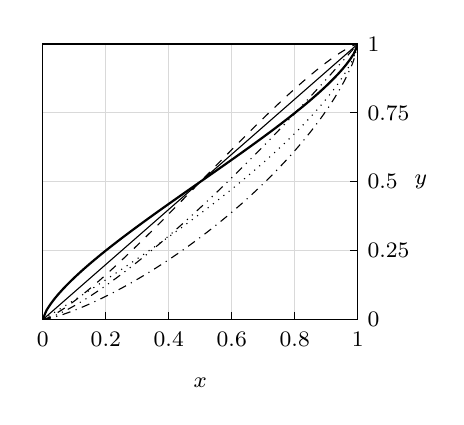
\begin{tikzpicture}
            \begin{scope}[every node/.append style = {font = \footnotesize}]
                \foreach \x in {0, 0.2, 0.4, 0.6, 0.8, 1}
                    \node at (4*\x,-0.25) {$\x$};
                \foreach \x in {0.2, 0.4, 0.6, 0.8} {
                    \draw[style = thin, gray!30!white] (4*\x,0) -- (4*\x,3.5);
                    \draw (4*\x,0) -- (4*\x,0.1);
                }
                \foreach \y in {0, 0.25, ..., 1}
                    \node[anchor = west] at (4,3.5*\y) {$\y$};
                \foreach \y in {0.25, 0.5, 0.75} {
                    \draw[style = thin, gray!30!white] (0,3.5*\y) -- (4,3.5*\y);
                    \draw (4,3.5*\y) -- (3.9,3.5*\y);
                }
                \node at (2,-0.8) {$x$};
                \node at (4.8,1.75) {$y$};
            \end{scope}
            \begin{scope}
            \draw[clip] (0,0) -- (4,0) -- (4,3.5) -- (0,3.5) -- cycle;
            \draw[style = thick] plot[smooth, tension = 0.7] coordinates{(0.,0.) (0.05,0.122729) (0.1,0.199686) (0.15,0.265642) (0.2,0.325421) (0.25,0.381049) (0.3,0.433623) (0.35,0.483822) (0.4,0.532106) (0.45,0.578801) (0.5,0.624154) (0.55,0.668352) (0.6,0.711547) (0.65,0.75386) (0.7,0.795393) (0.75,0.836229) (0.8,0.876442) (0.85,0.916092) (0.9,0.955234) (0.95,0.993916) (1.,1.03218) (1.05,1.07006) (1.1,1.1076) (1.15,1.14481) (1.2,1.18174) (1.25,1.21841) (1.3,1.25484) (1.35,1.29105) (1.4,1.32706) (1.45,1.3629) (1.5,1.39857) (1.55,1.43411) (1.6,1.46951) (1.65,1.50481) (1.7,1.54001) (1.75,1.57513) (1.8,1.61018) (1.85,1.64518) (1.9,1.68014) (1.95,1.71508) (2.,1.75) (2.05,1.78492) (2.1,1.81986) (2.15,1.85482) (2.2,1.88982) (2.25,1.92487) (2.3,1.95999) (2.35,1.99519) (2.4,2.03049) (2.45,2.06589) (2.5,2.10143) (2.55,2.1371) (2.6,2.17294) (2.65,2.20895) (2.7,2.24516) (2.75,2.28159) (2.8,2.31826) (2.85,2.35519) (2.9,2.3924) (2.95,2.42994) (3.,2.46782) (3.05,2.50608) (3.1,2.54477) (3.15,2.58391) (3.2,2.62356) (3.25,2.66377) (3.3,2.70461) (3.35,2.74614) (3.4,2.78845) (3.45,2.83165) (3.5,2.87585) (3.55,2.9212) (3.6,2.96789) (3.65,3.01618) (3.7,3.06638) (3.75,3.11895) (3.8,3.17458) (3.85,3.23436) (3.9,3.30031) (3.95,3.37727) (4.,3.5)};
            \draw plot[smooth, tension = 0.7] coordinates{(0.,0.) (0.05,0.04375) (0.1,0.0875) (0.15,0.13125) (0.2,0.175) (0.25,0.21875) (0.3,0.2625) (0.35,0.30625) (0.4,0.35) (0.45,0.39375) (0.5,0.4375) (0.55,0.48125) (0.6,0.525) (0.65,0.56875) (0.7,0.6125) (0.75,0.65625) (0.8,0.7) (0.85,0.74375) (0.9,0.7875) (0.95,0.83125) (1.,0.875) (1.05,0.91875) (1.1,0.9625) (1.15,1.00625) (1.2,1.05) (1.25,1.09375) (1.3,1.1375) (1.35,1.18125) (1.4,1.225) (1.45,1.26875) (1.5,1.3125) (1.55,1.35625) (1.6,1.4) (1.65,1.44375) (1.7,1.4875) (1.75,1.53125) (1.8,1.575) (1.85,1.61875) (1.9,1.6625) (1.95,1.70625) (2.,1.75) (2.05,1.79375) (2.1,1.8375) (2.15,1.88125) (2.2,1.925) (2.25,1.96875) (2.3,2.0125) (2.35,2.05625) (2.4,2.1) (2.45,2.14375) (2.5,2.1875) (2.55,2.23125) (2.6,2.275) (2.65,2.31875) (2.7,2.3625) (2.75,2.40625) (2.8,2.45) (2.85,2.49375) (2.9,2.5375) (2.95,2.58125) (3.,2.625) (3.05,2.66875) (3.1,2.7125) (3.15,2.75625) (3.2,2.8) (3.25,2.84375) (3.3,2.8875) (3.35,2.93125) (3.4,2.975) (3.45,3.01875) (3.5,3.0625) (3.55,3.10625) (3.6,3.15) (3.65,3.19375) (3.7,3.2375) (3.75,3.28125) (3.8,3.325) (3.85,3.36875) (3.9,3.4125) (3.95,3.45625) (4.,3.5)};
            \draw[style = dashed] plot[smooth, tension = 0.7] coordinates{(0.,0.) (0.05,0.016009) (0.1,0.0393343) (0.15,0.0664891) (0.2,0.0964324) (0.25,0.128603) (0.3,0.162638) (0.35,0.19828) (0.4,0.235336) (0.45,0.27365) (0.5,0.313099) (0.55,0.353577) (0.6,0.394995) (0.65,0.437275) (0.7,0.48035) (0.75,0.52416) (0.8,0.568649) (0.85,0.613768) (0.9,0.659473) (0.95,0.705723) (1.,0.752478) (1.05,0.799703) (1.1,0.847365) (1.15,0.895432) (1.2,0.943875) (1.25,0.992665) (1.3,1.04178) (1.35,1.09118) (1.4,1.14086) (1.45,1.19078) (1.5,1.24092) (1.55,1.29127) (1.6,1.3418) (1.65,1.39248) (1.7,1.4433) (1.75,1.49424) (1.8,1.54528) (1.85,1.59639) (1.9,1.64756) (1.95,1.69877) (2.,1.75) (2.05,1.80123) (2.1,1.85244) (2.15,1.90361) (2.2,1.95472) (2.25,2.00576) (2.3,2.0567) (2.35,2.10752) (2.4,2.1582) (2.45,2.20873) (2.5,2.25908) (2.55,2.30922) (2.6,2.35914) (2.65,2.40882) (2.7,2.45822) (2.75,2.50733) (2.8,2.55613) (2.85,2.60457) (2.9,2.65264) (2.95,2.7003) (3.,2.74752) (3.05,2.79428) (3.1,2.84053) (3.15,2.88623) (3.2,2.93135) (3.25,2.97584) (3.3,3.01965) (3.35,3.06272) (3.4,3.10501) (3.45,3.14642) (3.5,3.1869) (3.55,3.22635) (3.6,3.26466) (3.65,3.30172) (3.7,3.33736) (3.75,3.3714) (3.8,3.40357) (3.85,3.43351) (3.9,3.46067) (3.95,3.48399) (4.,3.5)};
            \draw[style = dotted] plot[smooth, tension = 0.7] coordinates{(0.,0.) (0.05,0.0306827) (0.1,0.0614822) (0.15,0.0924004) (0.2,0.123439) (0.25,0.154601) (0.3,0.185887) (0.35,0.217301) (0.4,0.248844) (0.45,0.280519) (0.5,0.312328) (0.55,0.344273) (0.6,0.376358) (0.65,0.408584) (0.7,0.440955) (0.75,0.473474) (0.8,0.506143) (0.85,0.538966) (0.9,0.571945) (0.95,0.605084) (1.,0.638387) (1.05,0.671856) (1.1,0.705497) (1.15,0.739311) (1.2,0.773304) (1.25,0.80748) (1.3,0.841843) (1.35,0.876397) (1.4,0.911147) (1.45,0.946098) (1.5,0.981256) (1.55,1.01662) (1.6,1.05221) (1.65,1.08802) (1.7,1.12406) (1.75,1.16033) (1.8,1.19685) (1.85,1.23362) (1.9,1.27064) (1.95,1.30793) (2.,1.3455) (2.05,1.38334) (2.1,1.42148) (2.15,1.45992) (2.2,1.49868) (2.25,1.53776) (2.3,1.57717) (2.35,1.61694) (2.4,1.65706) (2.45,1.69757) (2.5,1.73847) (2.55,1.77978) (2.6,1.82152) (2.65,1.86371) (2.7,1.90637) (2.75,1.94953) (2.8,1.99321) (2.85,2.03744) (2.9,2.08225) (2.95,2.12767) (3.,2.17375) (3.05,2.22052) (3.1,2.26804) (3.15,2.31636) (3.2,2.36554) (3.25,2.41565) (3.3,2.46678) (3.35,2.51901) (3.4,2.57246) (3.45,2.62727) (3.5,2.6836) (3.55,2.74164) (3.6,2.80166) (3.65,2.86398) (3.7,2.92903) (3.75,2.99744) (3.8,3.07012) (3.85,3.14853) (3.9,3.23538) (3.95,3.33711) (4.,3.5)};
            \draw[style = dashdotted] plot[smooth, tension = 0.7] coordinates{(0.,0.) (0.05,0.00777533) (0.1,0.0191863) (0.15,0.0325726) (0.2,0.0474487) (0.25,0.0635576) (0.3,0.0807371) (0.35,0.0988743) (0.4,0.117886) (0.45,0.137708) (0.5,0.15829) (0.55,0.179591) (0.6,0.201577) (0.65,0.22422) (0.7,0.247495) (0.75,0.271384) (0.8,0.295868) (0.85,0.320933) (0.9,0.346566) (0.95,0.372757) (1.,0.399496) (1.05,0.426775) (1.1,0.454588) (1.15,0.482929) (1.2,0.511794) (1.25,0.541179) (1.3,0.571081) (1.35,0.601499) (1.4,0.632432) (1.45,0.663879) (1.5,0.69584) (1.55,0.728317) (1.6,0.761311) (1.65,0.794825) (1.7,0.828861) (1.75,0.863424) (1.8,0.898518) (1.85,0.934147) (1.9,0.970318) (1.95,1.00704) (2.,1.04431) (2.05,1.08215) (2.1,1.12056) (2.15,1.15955) (2.2,1.19914) (2.25,1.23933) (2.3,1.28013) (2.35,1.32157) (2.4,1.36365) (2.45,1.4064) (2.5,1.44983) (2.55,1.49396) (2.6,1.53881) (2.65,1.5844) (2.7,1.63077) (2.75,1.67793) (2.8,1.72593) (2.85,1.77479) (2.9,1.82456) (2.95,1.87527) (3.,1.92697) (3.05,1.97972) (3.1,2.03357) (3.15,2.08859) (3.2,2.14486) (3.25,2.20247) (3.3,2.26151) (3.35,2.32211) (3.4,2.3844) (3.45,2.44855) (3.5,2.51477) (3.55,2.5833) (3.6,2.65446) (3.65,2.72866) (3.7,2.80643) (3.75,2.88855) (3.8,2.97614) (3.85,3.07101) (3.9,3.17651) (3.95,3.30056) (4.,3.5)};
            \draw[style = dashdotdotted] plot[smooth, tension = 0.7] coordinates{(0.,0.) (0.05,0.0117504) (0.1,0.0289328) (0.15,0.0490127) (0.2,0.0712408) (0.25,0.0952165) (0.3,0.120683) (0.35,0.147461) (0.4,0.175416) (0.45,0.20444) (0.5,0.23445) (0.55,0.265376) (0.6,0.297157) (0.65,0.329744) (0.7,0.363093) (0.75,0.397164) (0.8,0.431924) (0.85,0.467342) (0.9,0.503391) (0.95,0.540046) (1.,0.577285) (1.05,0.615086) (1.1,0.653432) (1.15,0.692305) (1.2,0.731688) (1.25,0.771566) (1.3,0.811926) (1.35,0.852754) (1.4,0.894039) (1.45,0.935769) (1.5,0.977932) (1.55,1.02052) (1.6,1.06352) (1.65,1.10693) (1.7,1.15073) (1.75,1.19492) (1.8,1.23949) (1.85,1.28444) (1.9,1.32975) (1.95,1.37542) (2.,1.42144) (2.05,1.46781) (2.1,1.51452) (2.15,1.56156) (2.2,1.60894) (2.25,1.65664) (2.3,1.70465) (2.35,1.75299) (2.4,1.80163) (2.45,1.85057) (2.5,1.89982) (2.55,1.94936) (2.6,1.9992) (2.65,2.04932) (2.7,2.09973) (2.75,2.15042) (2.8,2.20138) (2.85,2.25262) (2.9,2.30413) (2.95,2.35591) (3.,2.40795) (3.05,2.46025) (3.1,2.51281) (3.15,2.56563) (3.2,2.6187) (3.25,2.67201) (3.3,2.72558) (3.35,2.77938) (3.4,2.83343) (3.45,2.88772) (3.5,2.94224) (3.55,2.997) (3.6,3.05199) (3.65,3.10721) (3.7,3.16266) (3.75,3.21833) (3.8,3.27423) (3.85,3.33034) (3.9,3.38668) (3.95,3.44323) (4.,3.5)};
            \end{scope}
        \end{tikzpicture}
    }

    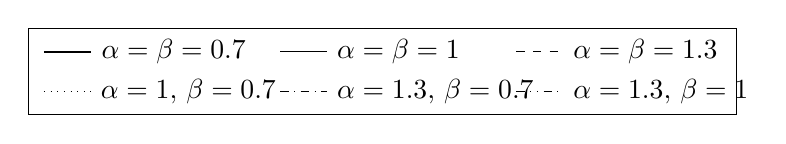
\begin{tikzpicture}
        \draw (0,1.9) -- (9,1.9) -- (9,3) -- (0,3) -- cycle;
        \draw[style = thick] (0.2,2.7) -- (0.8,2.7) node[right] {$\alpha=\beta=0.7$};
        \draw (3.2,2.7) -- (3.8,2.7) node[right] {$\alpha=\beta=1$};
        \draw[style = dashed] (6.2,2.7) -- (6.8,2.7) node[right] {$\alpha=\beta=1.3$};
        \draw[style = dotted] (0.2,2.2) -- (0.8,2.2) node[right] {$\alpha=1,\,\beta=0.7$};
        \draw[style = dashdotted] (3.2,2.2) -- (3.8,2.2) node[right] {$\alpha=1.3,\,\beta=0.7$};
        \draw[style = dashdotdotted] (6.2,2.2) -- (6.8,2.2) node[right] {$\alpha=1.3,\,\beta=1$};
    \end{tikzpicture}
    \caption{각종 불완전 베타함수의 그래프. 불완전 베타함수 $y=\Be(x;\alpha,\,\beta)$ (위), 정규화된 불완전 베타함수 $y=I_x(\alpha,\,\beta)$ (아래).}
\end{figure}

이제 베타함수의 성질을 살펴보아야 하는데, 앞서 베타함수의 well-definedness를 위해 보인 명제 \ref{prop:betaWellDefine}의 증명 과정에서 이미 가장 중요한 성질을 보였으므로, 여기에서는 결과만 다시 정리해 두도록 하겠다.

\begin{corollary}
    임의의 $x,\,y>0$에 대해 다음이 성립한다.
    \begin{enumerate}
        \item $\Be(x,\,y)=\Gamma(x)\Gamma(y)/\Gamma(x+y)$
        \item $\Be(x,\,y)=\Be(y,\,x)$
    \end{enumerate}
\end{corollary}

\begin{proof}
    i은 명제 \ref{prop:betaWellDefine}의 증명으로부터 자명하고, ii는 i로부터 자명하다.
\end{proof}

그리고 이러한 성질을 이용하여 베타함수를 $\mathbb{R}^n$에서의 함수로 확장할 수 있다.

\begin{definition}
    $2$ 이상인 임의의 $n\in\mathbb{N}$에 대해 \textbf{다변수 베타함수(multivariate beta function)}를 $\Be_n:(\mathbb{R}^+)^n\to\mathbb{R}^+$로 쓰고 $\Be_n:x\mapsto\prod_{i=1}^n\Gamma(x_i)/\Gamma(\sum_{i=1}^nx_i)$로 정의한다.
\end{definition}

\subsection{Zeta function}

\begin{proposition}
    임의의 $\alpha\in\mathbb{R}$에 대해 $S(\alpha)=\sum_{k=1}^\infty k^{-\alpha}$라 하면 $\alpha>1$일때 $S(\alpha)<\infty$이고 그렇지 않으면 $S(\alpha)=\infty$이다.
\end{proposition}

\begin{proof}
    우선 $\int_1^\infty x^{-1}\,dx=[\log x]_1^\infty=\infty$이므로 적분판정법으로부터 $S(1)=\infty$이고, 곧 비교판정법으로부터 $\alpha\leq1$이면 $S(\alpha)\geq S(1)=\infty$이다. 한편, $\alpha>1$이면 $\int_1^\infty x^{-\alpha}\,dx=[x^{1-\alpha}/(1-\alpha)]^\infty_1=(\alpha-1)^{-1}<\infty$이므로 다시 적분판정법으로부터 $S(\alpha)<\infty$이다.
\end{proof}

\begin{definition}
    다음과 같이 정의되는 함수 $\zeta:(1,\,\infty)\to\mathbb{R}^+$를 \textbf{(Riemann) 제타함수(- zeta function)}라 한다.
    \begin{equation*}
        \zeta:x\mapsto\sum_{k=1}^\infty\frac{1}{k^x}
    \end{equation*}
\end{definition}

\begin{figure}[!ht]
    \centering
    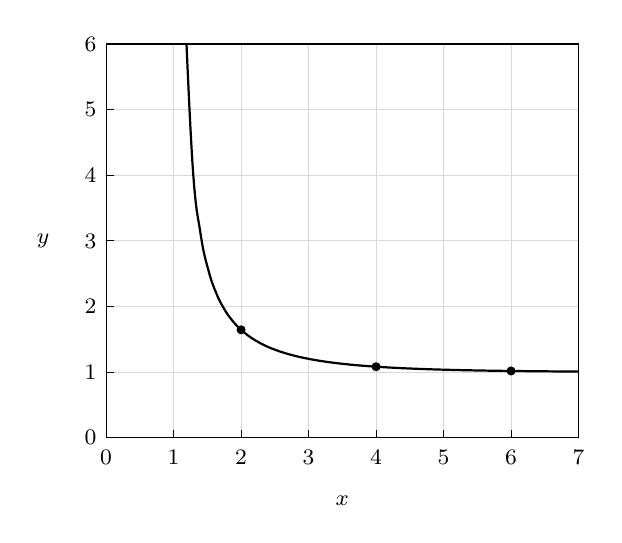
\begin{tikzpicture}
        \begin{scope}[every node/.append style = {font = \footnotesize}]
            \foreach \x in {0, ..., 7}
                \node at (6*\x/7,-0.25) {$\x$};
            \foreach \x in {1, ..., 6} {
                \draw[style = thin, gray!30!white] (6*\x/7,0) -- (6*\x/7,5);
                \draw (6*\x/7,0) -- (6*\x/7,0.1);
            }
            \foreach \y in {0, ..., 6}
                \node[anchor = east] at (0,5*\y/6) {$\y$};
            \foreach \y in {1, ..., 5} {
                \draw[style = thin, gray!30!white] (0,5*\y/6) -- (6,5*\y/6);
                \draw (0,5*\y/6) -- (0.1,5*\y/6);
            }
            \node at (3,-0.8) {$x$};
            \node at (-0.8,2.5) {$y$};
        \end{scope}
        \begin{scope}
        \draw[clip] (0,0) -- (6,0) -- (6,5) -- (0,5) -- cycle;
        \draw[style = thick] plot[smooth, tension = 0.7] coordinates{(1.,5.49101) (1.1,3.43905) (1.2,2.58796) (1.3,2.12416) (1.4,1.83355) (1.5,1.63527) (1.6,1.49197) (1.7,1.38403) (1.8,1.30018) (1.9,1.23344) (2.,1.1793) (2.1,1.13467) (2.2,1.09742) (2.3,1.06598) (2.4,1.03919) (2.5,1.0162) (2.6,0.99632) (2.7,0.979033) (2.8,0.963921) (2.9,0.950649) (3.,0.938945) (3.1,0.928586) (3.2,0.919388) (3.3,0.911196) (3.4,0.903881) (3.5,0.897333) (3.6,0.89146) (3.7,0.88618) (3.8,0.881427) (3.9,0.877139) (4.,0.873266) (4.1,0.869763) (4.2,0.86659) (4.3,0.863712) (4.4,0.8611) (4.5,0.858727) (4.6,0.856568) (4.7,0.854603) (4.8,0.852813) (4.9,0.851181) (5.,0.849691) (5.1,0.848332) (5.2,0.84709) (5.3,0.845955) (5.4,0.844917) (5.5,0.843967) (5.6,0.843098) (5.7,0.842302) (5.8,0.841572) (5.9,0.840904) (6.,0.840291)};
        \end{scope}
        \draw[fill = black] (12/7,5*1.64493/6) circle[radius = 0.05];
        \draw[fill = black] (24/7,5*1.08232/6) circle[radius = 0.05];
        \draw[fill = black] (36/7,5*1.01734/6) circle[radius = 0.05];
    \end{tikzpicture}
\end{figure}

\begin{figure}[!ht]
    \makebox[\linewidth][c]{
        \centering
        \subfigure{
            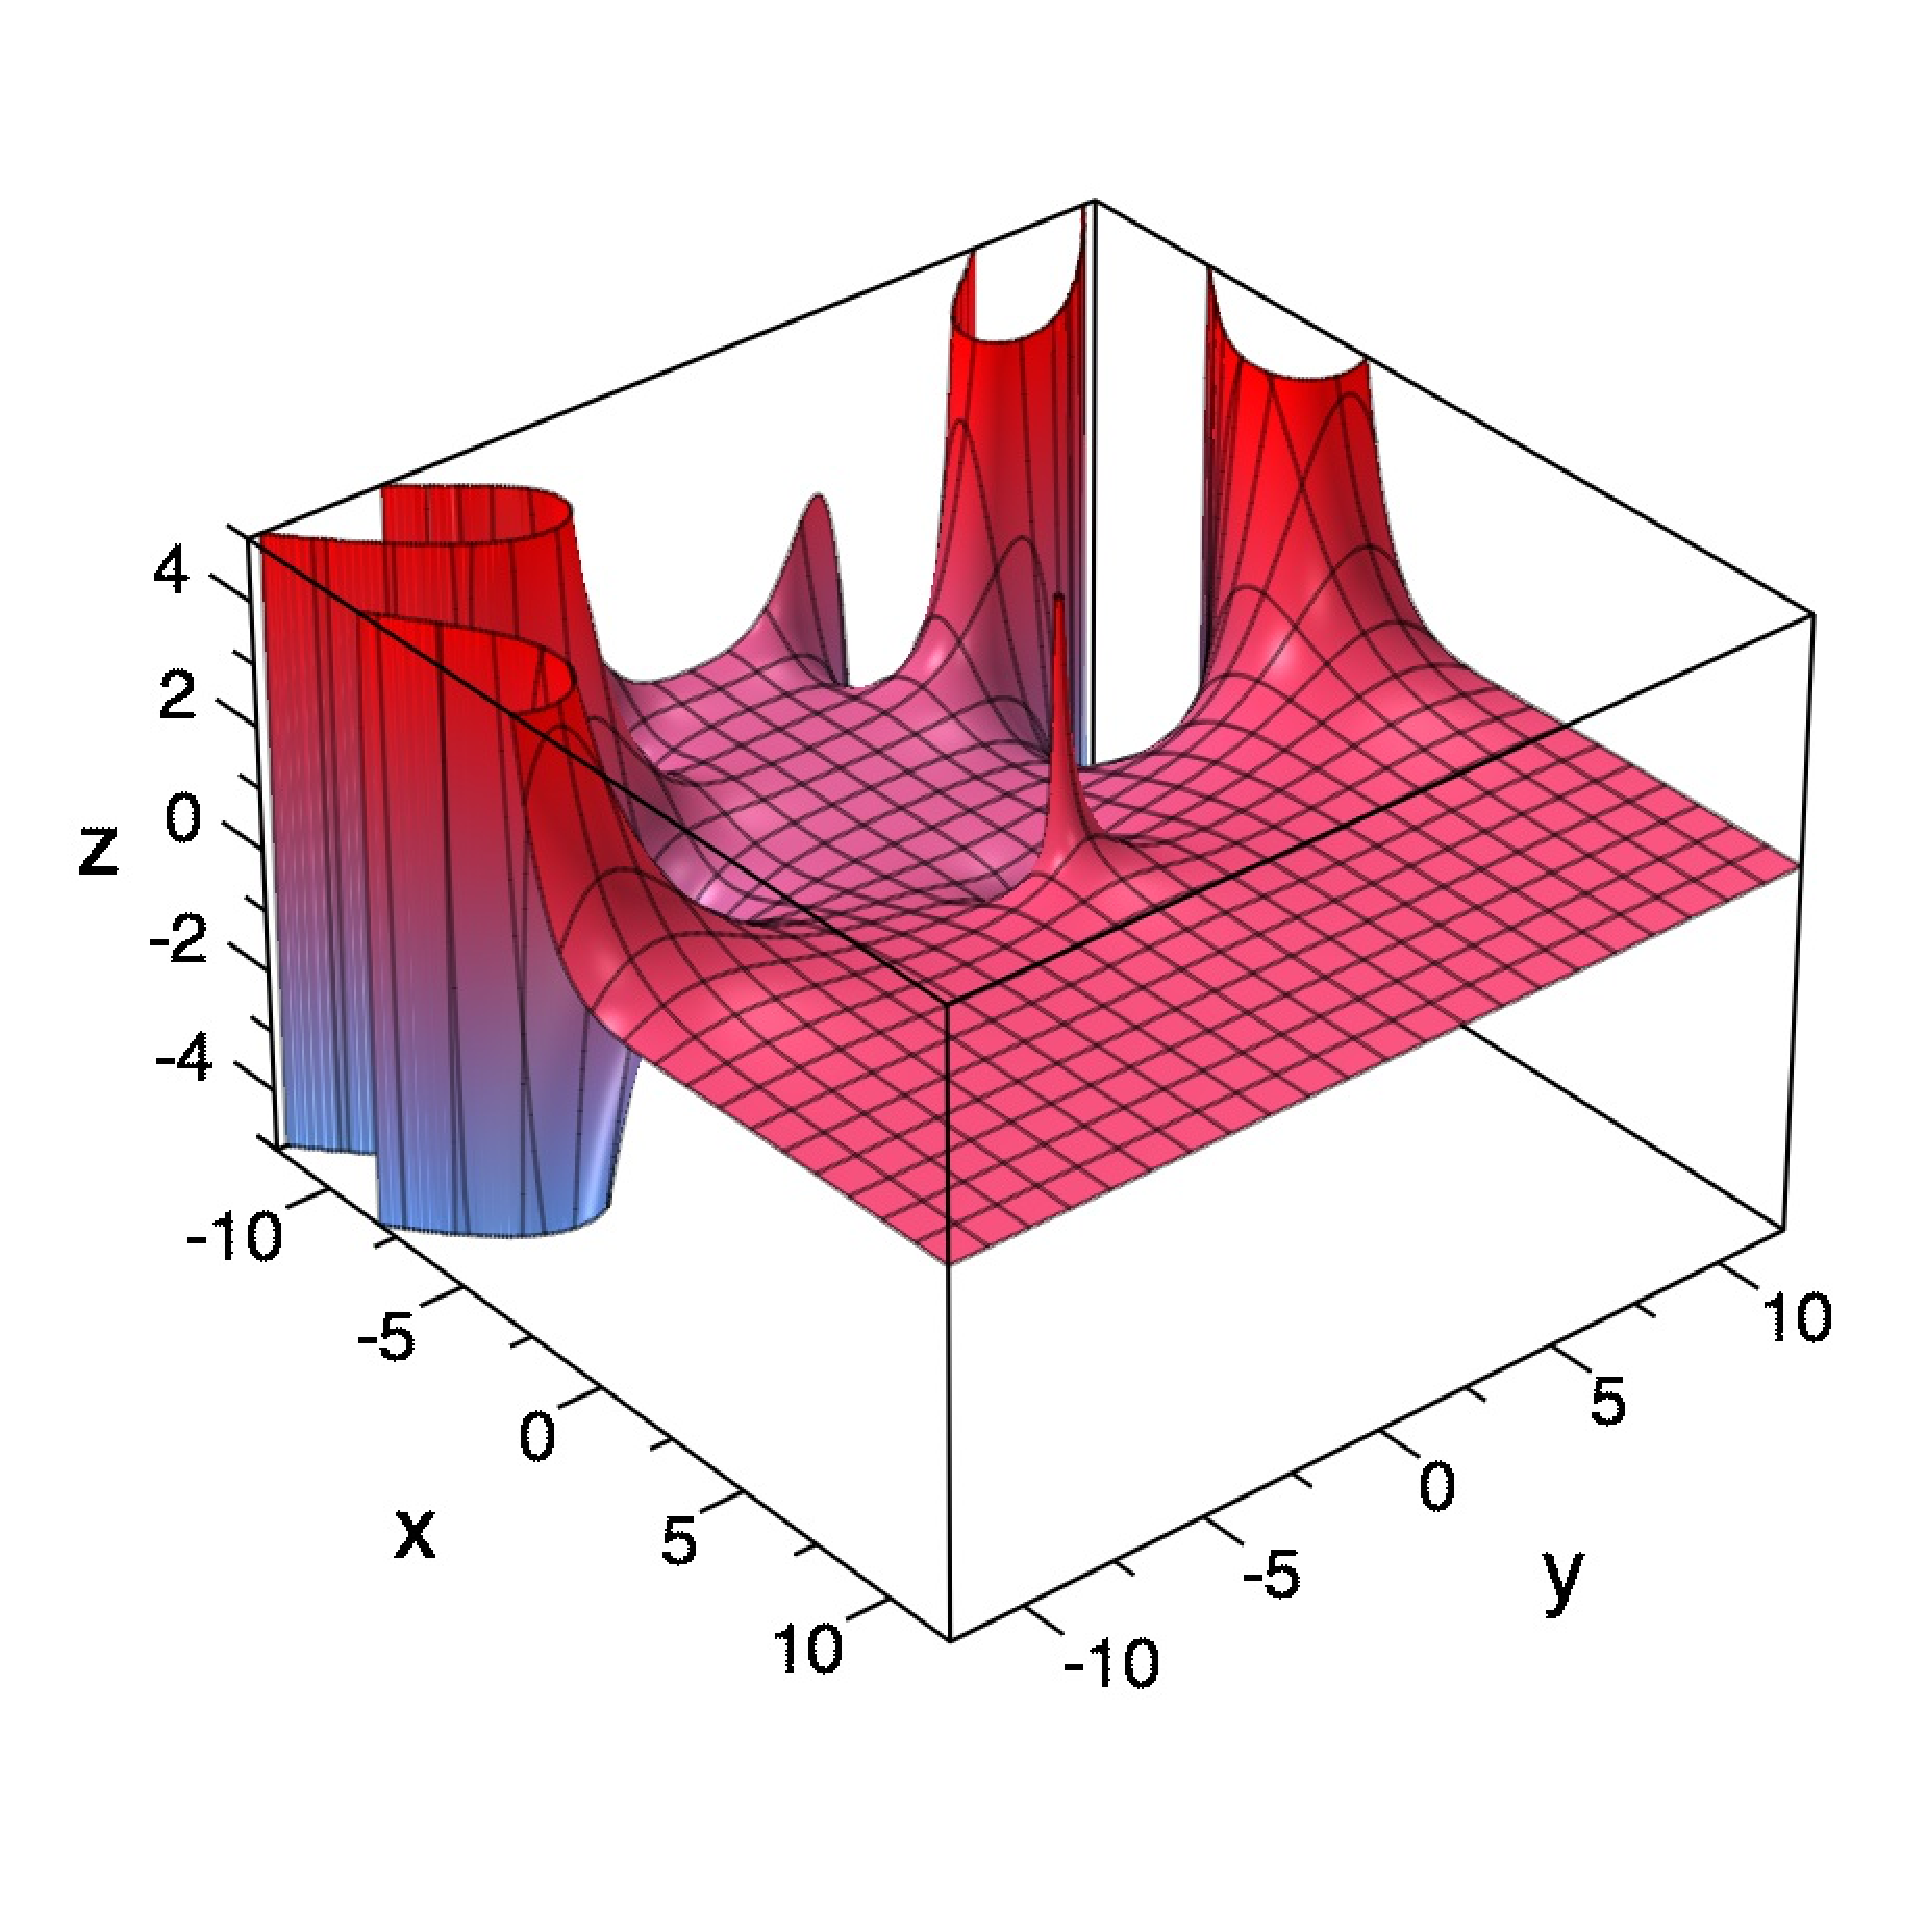
\includegraphics[width = 0.45\textwidth]{ZetaFuncRe.eps}
        }
        \subfigure{
            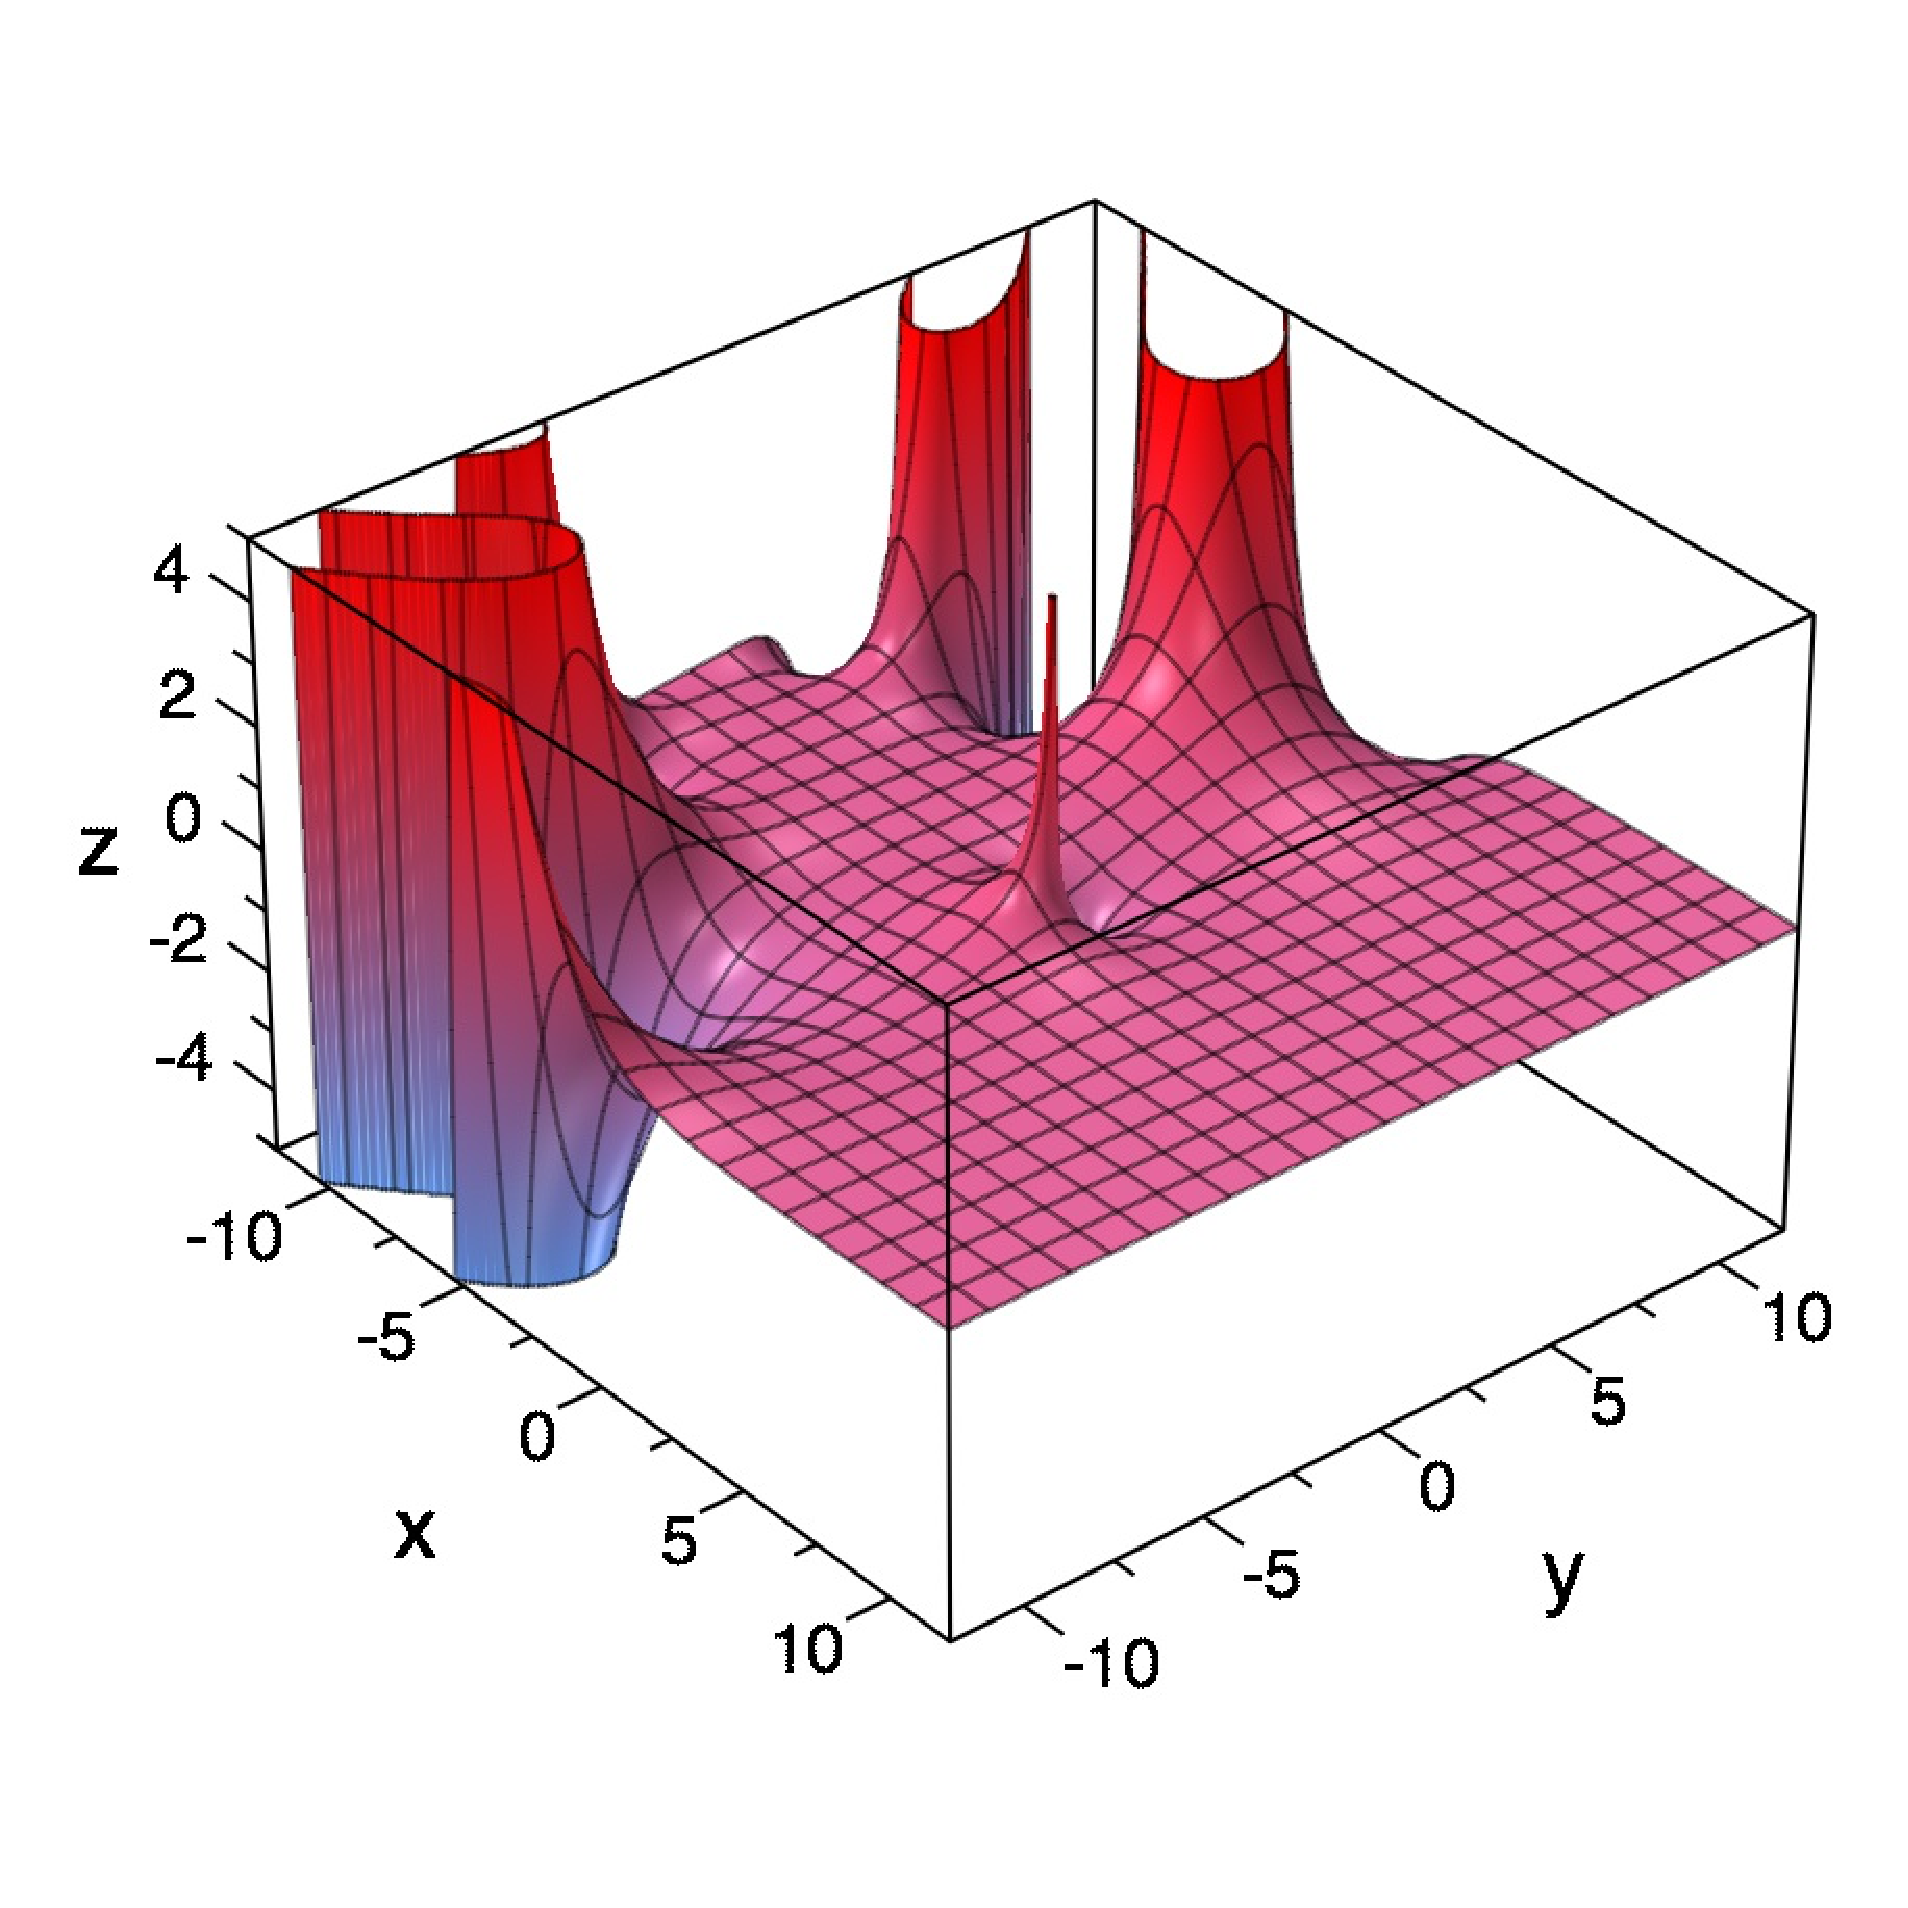
\includegraphics[width = 0.45\textwidth]{ZetaFuncIm.eps}
        }
        \subfigure{
            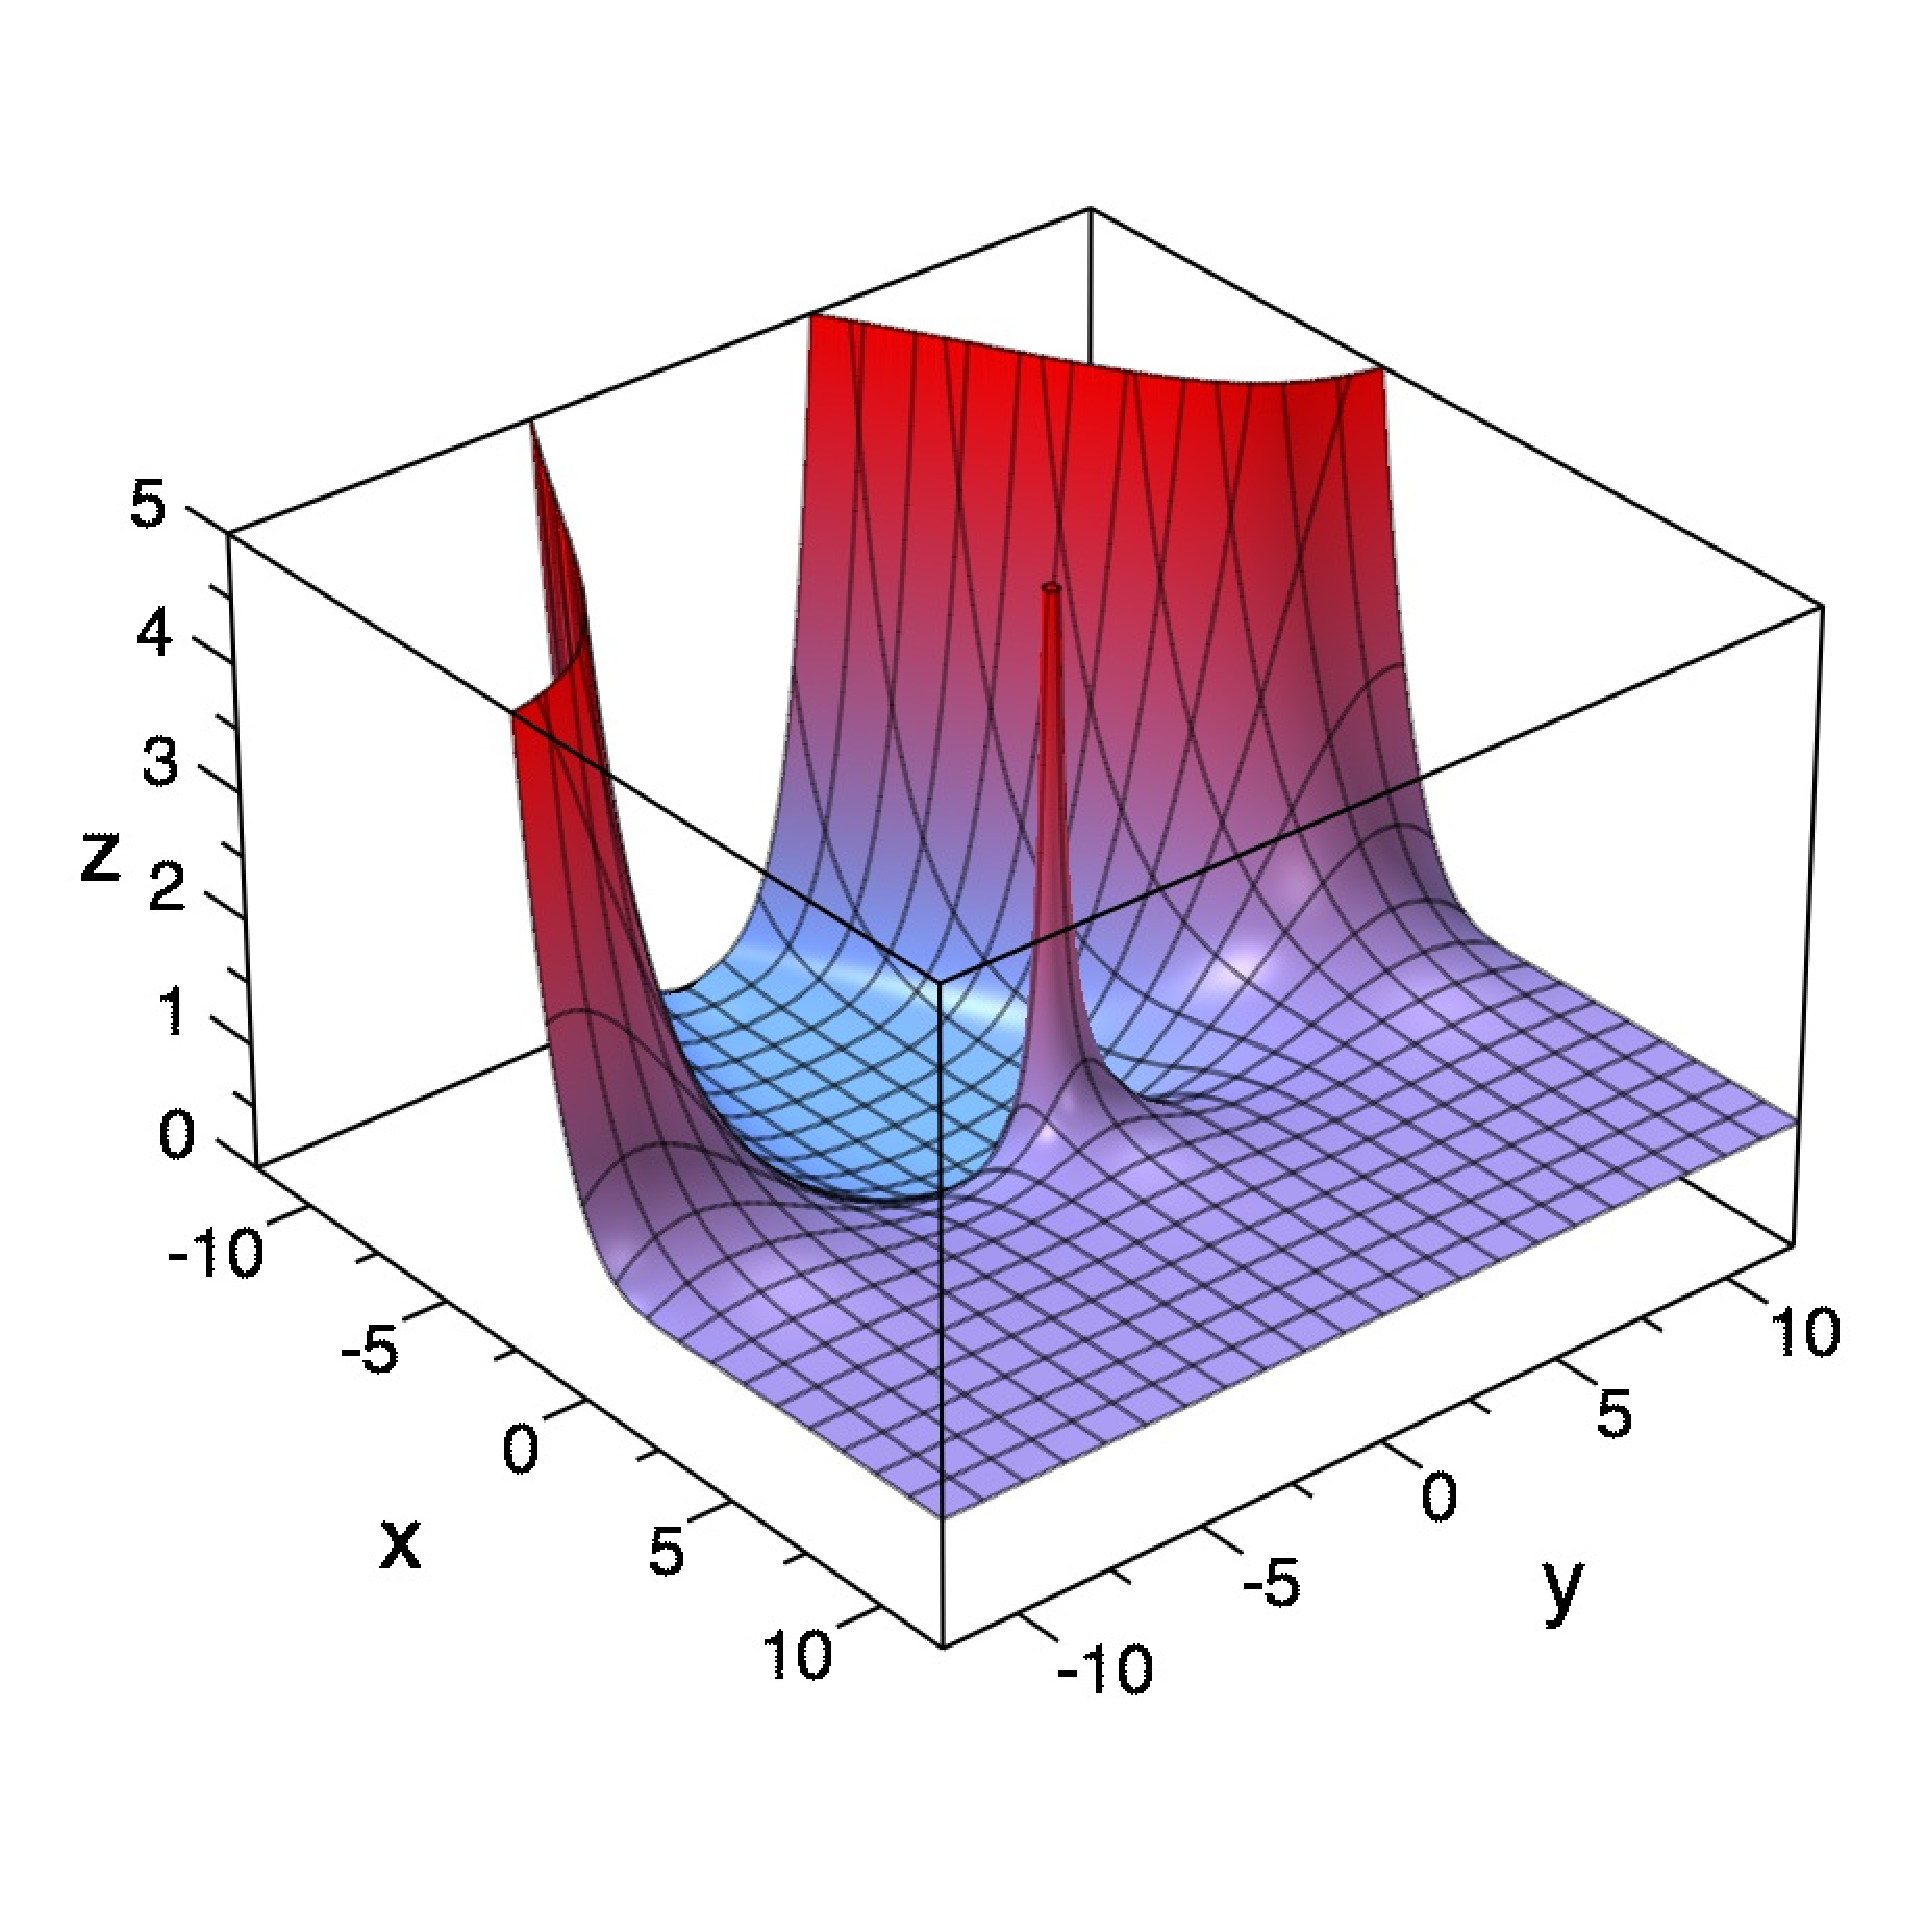
\includegraphics[width = 0.45\textwidth]{ZetaFuncAbs.eps}
        }
    }
    \caption{제타함수 $\zeta(x)$의 그래프.}
\end{figure}

\begin{proposition}
    함수 $f:\mathbb{R}\to\mathbb{R}$를
    \begin{equation*}
        f:x\mapsto
        \begin{dcases*}
            x/(e^x-1)&$x\ne0$인 경우\\
            1&ow.
        \end{dcases*}
    \end{equation*}
    로 정의하면 이는 해석함수이다.
\end{proposition}

\begin{proof}
    함수 $g:\mathbb{R}\to\mathbb{R}$를
    \begin{equation*}
        g:x\mapsto
        \begin{dcases*}
            (e^x-1)/x&$x\ne0$인 경우\\
            1&ow.
        \end{dcases*}
    \end{equation*}
    로 두면 이가 $x\ne0$에서 해석적임은 자명하므로 $x=0$에서도 해석적임을 보이면 충분하다. 이를 위해, 임의의 $x\in\mathbb{R}$에 대해 $g(x)=\sum_{k=1}^\infty x^{k-1}/k!$임을 생각하면 (단, 여기서 $0^0=1$로 생각한다.) 이의 수렴반경이 $\infty$이고 각 항이 $\mathcal{C}^\infty$급 함수이므로 $g$ 또한 $\mathcal{C}^\infty$급 함수이며, 나아가 임의의 $n\in\mathbb{N}_0$에 대해 $g^{(n)}(0)$는 $x^n/n!$의 계수로 주어지므로 $g$가 $x=0$에서 해석적임을 안다.
\end{proof}

\begin{figure}[!ht]
    \centering
    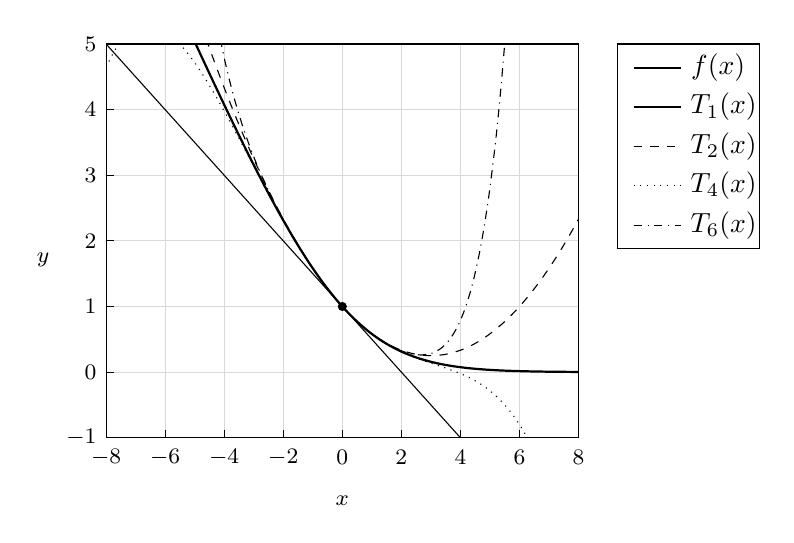
\begin{tikzpicture}
        \begin{scope}[every node/.append style = {font = \footnotesize}]
            \foreach \x in {-8, -6, ..., 8}
                \node at (3*\x/8,-5/6-0.25) {$\x$};
            \foreach \x in {-6, -4, ..., 6} {
                \draw[style = thin, gray!30!white] (3*\x/8,-5/6) -- (3*\x/8,25/6);
                \draw (3*\x/8,-5/6) -- (3*\x/8,-5/6+0.1);
            }
            \foreach \y in {-1, ..., 5}
                \node[anchor = east] at (-3,5*\y/6) {$\y$};
            \foreach \y in {0, ..., 4} {
                \draw[style = thin, gray!30!white] (-3,5*\y/6) -- (3,5*\y/6);
                \draw (-3,5*\y/6) -- (-2.9,5*\y/6);
            }
            \node at (0,-5/6-0.8) {$x$};
            \node at (-3.8,10/7) {$y$};
        \end{scope}
        \begin{scope}
        \draw[clip] (-3,-5/6) -- (3,-5/6) -- (3,25/6) -- (-3,25/6) -- cycle;
        \draw[style = thick] plot[smooth, tension = 0.7] coordinates{(-1.9,4.24901) (-1.8,4.03319) (-1.7,3.81881) (-1.6,3.60614) (-1.5,3.39552) (-1.4,3.18733) (-1.3,2.98199) (-1.2,2.77998) (-1.1,2.58185) (-1.,2.38816) (-0.9,2.19954) (-0.8,2.01663) (-0.7,1.84011) (-0.6,1.67063) (-0.5,1.50884) (-0.4,1.35533) (-0.3,1.21064) (-0.2,1.07522) (-0.1,0.949377) (0.,5/6) (0.1,0.727155) (0.2,0.630771) (0.3,0.543977) (0.4,0.466442) (0.5,0.397725) (0.6,0.337294) (0.7,0.284551) (0.8,0.238853) (0.9,0.199538) (1.,0.165938) (1.1,0.137404) (1.2,0.113318) (1.3,0.0931005) (1.4,0.0762186) (1.5,0.0621912) (1.6,0.0505887) (1.7,0.0410324) (1.8,0.0331922) (1.9,0.0267832) (2.,0.0215617) (2.1,0.0173207) (2.2,0.0138861) (2.3,0.0111118) (2.4,0.00887639) (2.5,0.0070792) (2.6,0.00563736) (2.7,0.00448286) (2.8,0.0035601) (2.9,0.00282379) (3.,0.00223717)};
        \draw (-3,25/6) -- (3/2,-5/6);
        \draw[style = dashed] plot[smooth, tension = 0.7] coordinates{(-1.8,4.43333) (-1.7,4.14938) (-1.6,3.87531) (-1.5,3.61111) (-1.4,3.35679) (-1.3,3.11235) (-1.2,2.87778) (-1.1,2.65309) (-1.,2.43827) (-0.9,2.23333) (-0.8,2.03827) (-0.7,1.85309) (-0.6,1.67778) (-0.5,1.51235) (-0.4,1.35679) (-0.3,1.21111) (-0.2,1.07531) (-0.1,0.949383) (0.,0.833333) (0.1,0.72716) (0.2,0.630864) (0.3,0.544444) (0.4,0.467901) (0.5,0.401235) (0.6,0.344444) (0.7,0.297531) (0.8,0.260494) (0.9,0.233333) (1.,0.216049) (1.1,0.208642) (1.2,0.211111) (1.3,0.223457) (1.4,0.245679) (1.5,0.277778) (1.6,0.319753) (1.7,0.371605) (1.8,0.433333) (1.9,0.504938) (2.,0.58642) (2.1,0.677778) (2.2,0.779012) (2.3,0.890123) (2.4,1.01111) (2.5,1.14198) (2.6,1.28272) (2.7,1.43333) (2.8,1.59383) (2.9,1.7642) (3.,1.94444)};
        \draw[style = dotted] plot[smooth, tension = 0.7] coordinates{(-3.,3.87037) (-2.9,4.06909) (-2.8,4.21861) (-2.7,4.32293) (-2.6,4.38592) (-2.5,4.41129) (-2.4,4.40264) (-2.3,4.36339) (-2.2,4.29686) (-2.1,4.20619) (-2.,4.09442) (-1.9,3.96442) (-1.8,3.81893) (-1.7,3.66055) (-1.6,3.49174) (-1.5,3.31481) (-1.4,3.13195) (-1.3,2.94518) (-1.2,2.75641) (-1.1,2.5674) (-1.,2.37974) (-0.9,2.19493) (-0.8,2.0143) (-0.7,1.83903) (-0.6,1.67019) (-0.5,1.50869) (-0.4,1.35529) (-0.3,1.21064) (-0.2,1.07521) (-0.1,0.949377) (0.,0.833333) (0.1,0.727155) (0.2,0.630771) (0.3,0.54397) (0.4,0.466403) (0.5,0.397577) (0.6,0.336859) (0.7,0.283478) (0.8,0.236521) (0.9,0.194933) (1.,0.157522) (1.1,0.122952) (1.2,0.0897481) (1.3,0.0562959) (1.4,0.0208391) (1.5,-0.0185185) (1.6,-0.0638138) (1.7,-0.117224) (1.8,-0.181067) (1.9,-0.2578) (2.,-0.350023) (2.1,-0.460474) (2.2,-0.592033) (2.3,-0.747721) (2.4,-0.930696)};
        \draw[style = dashdotted] plot[smooth, tension = 0.7] coordinates{(-1.6,4.48926) (-1.5,3.99206) (-1.4,3.57963) (-1.3,3.23217) (-1.2,2.93395) (-1.1,2.67273) (-1.,2.4392) (-0.9,2.22653) (-0.8,2.02988) (-0.7,1.84603) (-0.6,1.67297) (-0.5,1.50962) (-0.4,1.35554) (-0.3,1.21068) (-0.2,1.07522) (-0.1,0.949377) (0.,0.833333) (0.1,0.727155) (0.2,0.630774) (0.3,0.544014) (0.4,0.466646) (0.5,0.398506) (0.6,0.339633) (0.7,0.290473) (0.8,0.252107) (0.9,0.226531) (1.,0.216978) (1.1,0.228283) (1.2,0.267285) (1.3,0.343282) (1.4,0.46852) (1.5,0.65873) (1.6,0.933704) (1.7,1.31792) (1.8,1.84119) (1.9,2.53939) (2.,3.4552) (2.1,4.63889)};
        \end{scope}
        \draw (3.5,25/6-2.6) -- (5.3,25/6-2.6) -- (5.3,25/6) -- (3.5,25/6) -- cycle;
        \draw[style = thick] (3.7,25/6-0.3) -- (4.3,25/6-0.3) node[right] {$f(x)$};
        \draw (3.7,25/6-0.8) -- (4.3,25/6-0.8) node[right] {$T_1(x)$};
        \draw[style = dashed] (3.7,25/6-1.3) -- (4.3,25/6-1.3) node[right] {$T_2(x)$};
        \draw[style = dotted] (3.7,25/6-1.8) -- (4.3,25/6-1.8) node[right] {$T_4(x)$};
        \draw[style = dashdotted] (3.7,25/6-2.3) -- (4.3,25/6-2.3) node[right] {$T_6(x)$};
        \draw[fill = black] (0,5/6) circle[radius = 0.05];
    \end{tikzpicture}
    \caption{Bernoulli 수의 생성함수의 그래프.}
\end{figure}

\begin{definition}
    함수 $f:\mathbb{R}\to\mathbb{R}$를 다음과 같이 정의하자.
    \begin{equation*}
        f:x\mapsto
        \begin{dcases*}
            x/(e^x-1)&$x\ne0$인 경우\\
            1&ow.
        \end{dcases*}
    \end{equation*}
    이때, 이의 $0$에서의 Taylor 전개의 $n$차항의 계수를 $n$번째 \textbf{Bernoulli 수(- number)}라 하고 $B_n$으로 쓴다. 즉, $0$ 근방의 $x\in\mathbb{R}$에 대해 $f(x)=\sum_{k=0}^\infty B_kx^k/k!$이다. (단, 여기서 $0^0=1$로 생각한다.)
\end{definition}

\begin{table}
    \caption{Bernoulli 수}
    \begin{tabularx}{\textwidth}{C|CCCCCCCCC}
    \hline
    $n$ & $0$ & $1$ & $2$ & $3$ & $4$ & $5$ & $6$ & $7$ & $8$\\
    \svhline
    $B_n$ & $1$ & $-1/2$ & $1/6$ & $0$ & $-1/30$ & $0$ & $1/42$ & $0$ & $-1/30$\\
    \hline
    \end{tabularx}
\end{table}

\begin{theorem}\label{thm:bernoulliOdd}
    임의의 $n\in\mathbb{N}$에 대해
    \begin{equation*}
        B_{2n-1}=
        \begin{dcases*}
            -1/2&$n=1$인 경우\\
            0&ow.
        \end{dcases*}
    \end{equation*}
    이다.
\end{theorem}

\begin{proof}
    함수 $f$를 위의 정의에서와 같이 두면
    \begin{align*}
        B_1&=f'(0)\\
        &=\lim_{h\to0}\frac{f(h)-1}{h}\\
        &=\lim_{h\to0}\frac{h-e^h+1}{h(e^h-1)}\\
        &=\lim_{h\to0}\frac{1-e^h}{(h+1)e^h-1}\\
        &=-\lim_{h\to0}\frac{1}{h+2}\\
        &=-\frac{1}{2}
    \end{align*}
    이다. 여기서 네 번째와 다섯 번째 등호는 L'Hospital의 법칙으로부터 성립한다. 한편, 함수 $g:\mathbb{R}\to\mathbb{R}$를 $g:x\mapsto f(x)+x/2$로 두면 이는 우함수가 되어 임의의 $n\in\mathbb{N}$에 대해 $g^{(2n-1)}(0)=0$이고, 이로써 증명은 충분하다.
\end{proof}

\begin{definition}\label{def:bernoulliPoly}
    임의의 $x\in\mathbb{R}$에 대해 함수 $f_x:\mathbb{R}\to\mathbb{R}$를 다음과 같이 정의하자.
    \begin{equation*}
        f_x:t\mapsto
        \begin{dcases*}
            te^{xt}/(e^t-1)&$t\ne0$인 경우\\
            1&ow.
        \end{dcases*}
    \end{equation*}
    이때, 이의 $0$에서의 Taylor 전개의 $n$차항의 계수를 $n$번째 \textbf{Bernoulli 다항식(- polynomial)}이라 하고 $B_n(x)$로 쓴다. 즉, $0$ 근방의 $t\in\mathbb{R}$에 대해 $f_x(t)=\sum_{k=0}^\infty B_k(x)t^k/k!$이다. (단, 여기서 $0^0=1$로 생각한다.)
\end{definition}

\begin{figure}[!ht]
    \centering
    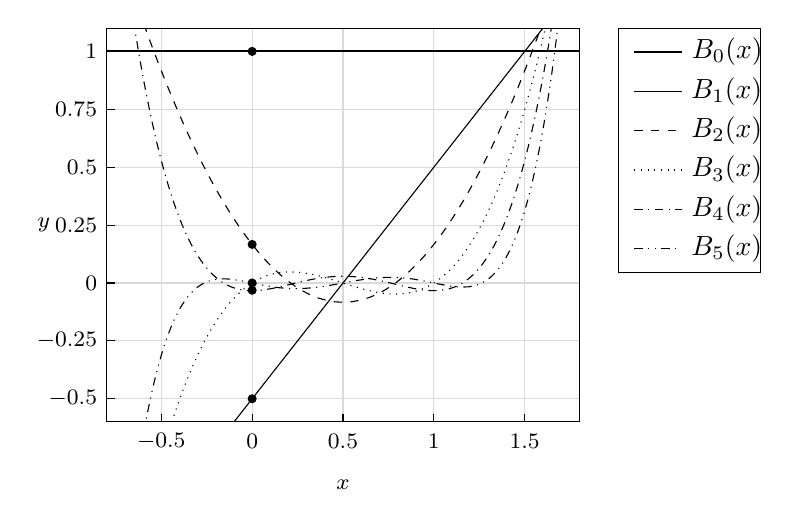
\begin{tikzpicture}
        \begin{scope}[every node/.append style = {font = \footnotesize}]
            \foreach \x in {-0.5, 0, ..., 1.5} {
                \node at (6*\x/2.6,-30/17-0.25) {$\x$};
                \draw[style = thin, gray!30!white] (6*\x/2.6,-30/17) -- (6*\x/2.6,55/17);
                \draw (6*\x/2.6,-30/17) -- (6*\x/2.6,-30/17+0.1);
            }
            \foreach \y in {-0.5, -0.25, ..., 1} {
                \node[anchor = east] at (-24/13,5*\y/1.7) {$\y$};
                \draw[style = thin, gray!30!white] (-24/13,5*\y/1.7) -- (54/13,5*\y/1.7);
                \draw (-24/13,5*\y/1.7) -- (-24/13+0.1,5*\y/1.7);
            }
            \node at (15/13,-30/17-0.8) {$x$};
            \node at (-24/13-0.8,25/34) {$y$};
        \end{scope}
        \begin{scope}
        \draw[clip] (-24/13,-30/17) -- (54/13,-30/17) -- (54/13,55/17) -- (-24/13,55/17) -- cycle;
        \draw[style = thick] (-24/13,5/1.7) -- (54/13,5/1.7);
        \draw (-0.230769,-30/17) -- (3.69231,55/17);
        \draw[style = dashed] plot[smooth, tension = 0.7] coordinates{(-1.44615,3.48837) (-1.34615,3.2067) (-1.24615,2.93608) (-1.14615,2.6765) (-1.04615,2.42797) (-0.946154,2.19049) (-0.846154,1.96405) (-0.746154,1.74866) (-0.646154,1.54431) (-0.546154,1.35101) (-0.446154,1.16876) (-0.346154,0.997549) (-0.246154,0.837386) (-0.146154,0.688268) (-0.0461538,0.550196) (0.0538462,0.42317) (0.153846,0.30719) (0.253846,0.202255) (0.353846,0.108366) (0.453846,0.0255229) (0.553846,-0.0462745) (0.653846,-0.107026) (0.753846,-0.156732) (0.853846,-0.195392) (0.953846,-0.223007) (1.05385,-0.239575) (1.15385,-0.245098) (1.25385,-0.239575) (1.35385,-0.223007) (1.45385,-0.195392) (1.55385,-0.156732) (1.65385,-0.107026) (1.75385,-0.0462745) (1.85385,0.0255229) (1.95385,0.108366) (2.05385,0.202255) (2.15385,0.30719) (2.25385,0.42317) (2.35385,0.550196) (2.45385,0.688268) (2.55385,0.837386) (2.65385,0.997549) (2.75385,1.16876) (2.85385,1.35101) (2.95385,1.54431) (3.05385,1.74866) (3.15385,1.96405) (3.25385,2.19049) (3.35385,2.42797) (3.45385,2.6765) (3.55385,2.93608) (3.65385,3.2067) (3.75385,3.48837)};
        \draw[style = dotted] plot[smooth, tension = 0.7] coordinates{(-1.04615,-1.84735) (-0.946154,-1.54727) (-0.846154,-1.27734) (-0.746154,-1.03614) (-0.646154,-0.822212) (-0.546154,-0.634135) (-0.446154,-0.47047) (-0.346154,-0.329779) (-0.246154,-0.210628) (-0.146154,-0.111581) (-0.0461538,-0.0312) (0.0538462,0.0319491) (0.153846,0.0793028) (0.253846,0.112297) (0.353846,0.132368) (0.453846,0.140951) (0.553846,0.139482) (0.653846,0.129398) (0.753846,0.112134) (0.853846,0.0891265) (0.953846,0.0618109) (1.05385,0.0316234) (1.15385,0) (1.25385,-0.0316234) (1.35385,-0.0618109) (1.45385,-0.0891265) (1.55385,-0.112134) (1.65385,-0.129398) (1.75385,-0.139482) (1.85385,-0.140951) (1.95385,-0.132368) (2.05385,-0.112297) (2.15385,-0.0793028) (2.25385,-0.0319491) (2.35385,0.0312) (2.45385,0.111581) (2.55385,0.210628) (2.65385,0.329779) (2.75385,0.47047) (2.85385,0.634135) (2.95385,0.822212) (3.05385,1.03614) (3.15385,1.27734) (3.25385,1.54727) (3.35385,1.84735) (3.45385,2.17902) (3.55385,2.54372) (3.65385,2.94288) (3.75385,3.37794)};
        \draw[style = dashdotted] plot[smooth, tension = 0.7] coordinates{(-1.54615,3.58413) (-1.44615,2.95823) (-1.34615,2.41095) (-1.24615,1.93596) (-1.14615,1.52714) (-1.04615,1.17865) (-0.946154,0.884901) (-0.846154,0.640527) (-0.746154,0.44043) (-0.646154,0.279757) (-0.546154,0.153903) (-0.446154,0.0585126) (-0.346154,-0.0105208) (-0.246154,-0.0570554) (-0.146154,-0.0847002) (-0.0461538,-0.0968152) (0.0538462,-0.0965118) (0.153846,-0.0866521) (0.253846,-0.0698498) (0.353846,-0.0484692) (0.453846,-0.024626) (0.553846,-0.00018698) (0.653846,0.0232301) (0.753846,0.0442562) (0.853846,0.0617714) (0.953846,0.0749045) (1.05385,0.0830332) (1.15385,0.0857843) (1.25385,0.0830332) (1.35385,0.0749045) (1.45385,0.0617714) (1.55385,0.0442562) (1.65385,0.0232301) (1.75385,-0.00018698) (1.85385,-0.024626) (1.95385,-0.0484692) (2.05385,-0.0698498) (2.15385,-0.0866521) (2.25385,-0.0965118) (2.35385,-0.0968152) (2.45385,-0.0847002) (2.55385,-0.0570554) (2.65385,-0.0105208) (2.75385,0.0585126) (2.85385,0.153903) (2.95385,0.279757) (3.05385,0.44043) (3.15385,0.640527) (3.25385,0.884901) (3.35385,1.17865) (3.45385,1.52714) (3.55385,1.93596) (3.65385,2.41095) (3.75385,2.95823) (3.85385,3.58413)};
        \draw[style = dashdotdotted] plot[smooth, tension = 0.7] coordinates{(-1.44615,-2.31742) (-1.34615,-1.73712) (-1.24615,-1.26745) (-1.14615,-0.893422) (-1.04615,-0.601332) (-0.946154,-0.37872) (-0.846154,-0.21431) (-0.746154,-0.0979608) (-0.646154,-0.0206101) (-0.546154,0.0257811) (-0.446154,0.0482806) (-0.346154,0.0530395) (-0.246154,0.0453459) (-0.146154,0.0296792) (-0.0461538,0.00976352) (0.0538462,-0.0113778) (0.153846,-0.0313687) (0.253846,-0.0484262) (0.353846,-0.0613069) (0.453846,-0.0692523) (0.553846,-0.0719357) (0.653846,-0.0694077) (0.753846,-0.0620426) (0.853846,-0.0504842) (0.953846,-0.0355921) (1.05385,-0.0183876) (1.15385,0) (1.25385,0.0183876) (1.35385,0.0355921) (1.45385,0.0504842) (1.55385,0.0620426) (1.65385,0.0694077) (1.75385,0.0719357) (1.85385,0.0692523) (1.95385,0.0613069) (2.05385,0.0484262) (2.15385,0.0313687) (2.25385,0.0113778) (2.35385,-0.00976352) (2.45385,-0.0296792) (2.55385,-0.0453459) (2.65385,-0.0530395) (2.75385,-0.0482806) (2.85385,-0.0257811) (2.95385,0.0206101) (3.05385,0.0979608) (3.15385,0.21431) (3.25385,0.37872) (3.35385,0.601332) (3.45385,0.893422) (3.55385,1.26745) (3.65385,1.73712) (3.75385,2.31742) (3.85385,3.02469) (3.95385,3.87669)};
        \end{scope}
        \draw (54/13+0.5,55/17-3.1) -- (54/13+2.3,55/17-3.1) -- (54/13+2.3,55/17) -- (54/13+0.5,55/17) -- cycle;
        \draw[style = thick] (54/13+0.7,55/17-0.3) -- (54/13+1.3,55/17-0.3) node[right] {$B_0(x)$};
        \draw (54/13+0.7,55/17-0.8) -- (54/13+1.3,55/17-0.8) node[right] {$B_1(x)$};
        \draw[style = dashed] (54/13+0.7,55/17-1.3) -- (54/13+1.3,55/17-1.3) node[right] {$B_2(x)$};
        \draw[style = dotted] (54/13+0.7,55/17-1.8) -- (54/13+1.3,55/17-1.8) node[right] {$B_3(x)$};
        \draw[style = dashdotted] (54/13+0.7,55/17-2.3) -- (54/13+1.3,55/17-2.3) node[right] {$B_4(x)$};
        \draw[style = dashdotdotted] (54/13+0.7,55/17-2.8) -- (54/13+1.3,55/17-2.8) node[right] {$B_5(x)$};
        \draw[fill = black] (0,-2.5/1.7) circle[radius = 0.05];
        \draw[fill = black] (0,-5/54) circle[radius = 0.05];
        \draw[fill = black] (0,0) circle[radius = 0.05];
        \draw[fill = black] (0,5/10.2) circle[radius = 0.05];
        \draw[fill = black] (0,5/1.7) circle[radius = 0.05];
    \end{tikzpicture}
    \caption{Bernoulli 다항식 $B_0(x),\,\cdots,\,B_5(x)$의 그래프.}
\end{figure}

\begin{theorem}\label{thm:bernouuliPolyExpansion}
    임의의 $n\in\mathbb{N}$과 임의의 $x\in\mathbb{R}$에 대해 다음이 성립하다. (단, 여기서 $0^0=1$로 생각한다.)
    \begin{equation*}
        B_n(x)=\sum_{k=0}^n\binom{n}{k}B_kx^{n-k}
    \end{equation*}
\end{theorem}

\begin{proof}
    임의의 $x\in\mathbb{R}$에 대해 함수 $f_x$를 위의 정의에서와 같이 두면 $0$ 근방의 $t\in\mathbb{R}$에 대해
    \begin{align*}
        \sum_{k=0}^\infty B_k(x)\frac{t^k}{k!}&=f_x(t)\\
        &=f_0(t)e^{xt}\\
        &=\bigg[\sum_{k=0}^\infty B_k\frac{t^k}{k!}\bigg]\bigg[\sum_{l=0}^\infty\frac{(xt)^l}{l!}\bigg]\\
        &=\sum_{m=0}^\infty\sum_{k=0}^mB_kx^{m-k}\frac{t^m}{k!(m-k)!}\\
        &=\sum_{m=0}^\infty\sum_{k=0}^m\binom{m}{k}B_kx^{m-k}\frac{t^m}{m!}
    \end{align*}
    이므로 양변에서 $t^n/n!$의 계수를 비교하면 증명이 끝난다.
\end{proof}

\begin{corollary}
    임의의 $n\in\mathbb{N}$에 대해 $B_n=B_n(0)$이다.
\end{corollary}

\begin{proof}
    이는 Bernoulli 수와 Bernoulli 다항식의 정의로부터 자명하다.
\end{proof}

\begin{lemma}[Newton's power sum formula]
    $n$차 다항식 $P(x)=\sum_{k=0}^na_kx^k$에 대해 방정식 $P(x)=0$의 $n$개의 근을 $\alpha_1,\,\cdots,\,\alpha_n\in\mathbb{C}$이라 하고 임의의 $i\in\mathbb{N}$에 대해 $S_i=\sum_{j=1}^n\alpha_j^i$라 하면 임의의 $k\in\mathbb{N}$에 대해
    \begin{equation*}
        \begin{dcases*}
            ka_{n-k}+\sum_{i=1}^ka_{n-k+i}S_i=0&when $k\leq n$\\
            \sum_{i=k-n}^ka_{n-k+i}S_i=0&ow.
        \end{dcases*}
    \end{equation*}
    이다.
\end{lemma}

\begin{proof}
    먼저 $\alpha_1,\,\cdots,\,\alpha_n$이 모두 $0$이 아닌 경우를 생각하면 이때 $a_0=\prod_{i=1}^n\alpha_i\ne0$이므로 다항식 $Q(x)=\sum_{k=0}^na_{n-k}x^k=x^nP(1/x)$를 생각하면 이는 $k$차 다항식이고 방정식 $Q(x)=0$는 $\alpha_1^{-1},\,\cdots,\,\alpha_n^{-1}$를 근으로 갖는다. 한편, $Q(x)=0$는 $0$을 근으로 갖지 않으므로 $0$의 적당한 근방 $I\subseteq\mathbb{R}$ 위에서 $Q$는 $0$이 아니어서 함수 $f:I\to\mathbb{R}$를 $f:x\mapsto\log|Q(x)|$로 정의하면 이는 well-define되며 $\mathcal{C}^\infty$급이다. 이로부터 임의의 $k\in\mathbb{N}$에 대해
    \begin{align*}
        f^{(k)}(x)&=\frac{d^k}{dx^k}\log\bigg(|a_0|\prod_{i=1}^n\bigg|x-\frac{1}{\alpha_i}\bigg|\bigg)\\
        &=\sum_{i=1}^n\frac{d^{k-1}}{dx^{k-1}}\frac{\alpha_i}{\alpha_ix-1}\\
        &=(-1)^{k-1}(k-1)!\sum_{i=1}^n\bigg(\frac{\alpha_i}{\alpha_ix-1}\bigg)^k
    \end{align*}
    이므로 $f^{(k)}(0)=-(k-1)!S_k$이고, 곧 임의의 $k\in\mathbb{N}$에 대해
    \begin{align*}
        \frac{Q^{(k)}(0)}{k!}&=\frac{(f'Q)^{(k-1)}(0)}{k!}\\
        &=\frac{1}{k!}\sum_{l=0}^{k-1}\binom{k-1}{l}f^{(l+1)}(0)Q^{(k-l-1)}(0)\\
        &=-\frac{1}{k!}\sum_{l=0}^{k-1}\binom{k-1}{l}l!S_{l+1}Q^{(k-l-1)}(0)\\
        &=-\frac{1}{k}\sum_{l=1}^k\frac{Q^{(k-l)}(0)}{(k-l)!}S_l
    \end{align*}
    인데 만약 $k\leq n$이면 이는 $ka_{n-k}+\sum_{i=1}^ka_{n-k+i}S_i=0$을 함의하고, 반대로 $k>n$이면 $\sum_{i=k-n}^ka_{n-k+i}S_i=0$을 함의하여 증명이 끝난다. 이제 일반적인 경우에 대해, $\alpha_1,\,\cdots,\,\alpha_n$ 중에서 $0$이 아닌 것의 개수를 $m\in\mathbb{N}_0$이라 하자. 만약 $m=0$이면, 즉 $\alpha_1=\cdots=\alpha_n=0$이면 보조정리가 자명하므로 $m>0$이라 하고, WLOG, 필요하다면 relabel하여 $\alpha_1,\,\cdots,\,\alpha_m$이 $0$이 아니라 하자. 그렇다면 $m$차 다항식 $\widetilde{P}(x)=\sum_{k=0}^ma_{k+n-m}x^k=P(x)/x^{n-m}$에 대해 방정식 $\widetilde{P}(x)=0$은 모두 $0$이 아닌 $\alpha_1,\,\cdots,\,\alpha_m$을 근으로 가지므로 앞선 결론으로부터
    \begin{equation*}
        \begin{dcases*}
            ka_{n-k}+\sum_{i=1}^ka_{n-k+i}S_i=0&when $k\leq m$\\
            \sum_{i=k-m}^ka_{n-k+i}S_i=0&ow.
        \end{dcases*}
    \end{equation*}
    이고, 가정으로부터 $a_0=\cdots=a_{n-m-1}=0$이므로 보조정리가 성립함을 안다.
\end{proof}

\begin{lemma}\label{lem:bernoulliSum}
    임의의 $n\in\mathbb{N}$에 대해 다음이 성립한다.
    \begin{equation*}
        \sum_{k=0}^n\frac{2^{2k}B_{2k}}{(2k)!(2n+1-2k)!}=\frac{1}{(2n)!}
    \end{equation*}
\end{lemma}

\begin{proof}
    임의의 $x\in\mathbb{R}$에 대해 함수 $f_x$를 정의 \ref{def:bernoulliPoly}에서와 같이 정의하면 $0$ 근방의 $t\in\mathbb{R}$에 대해 $\sum_{k=0}^\infty B_k(1-x)t^k/k!=f_{1-x}(t)=f_x(-t)=\sum_{k=0}^\infty(-1)^kB_k(x)t^k/k!$이므로 (단, 여기서 $0^0=1$로 생각한다.) 임의의 $n\in\mathbb{N}$에 대해 양변의 $t^n/n!$의 계수를 비교하면 $B_n(1-x)=(-1)^nB_n(x)$가 성립함을 알고, 곧 $B_{2n+1}(1/2)=-B_{2n+1}(1/2)$에서 $B_{2n+1}(1/2)=0$이다. 그렇다면 정리 \ref{thm:bernoulliOdd}, \ref{thm:bernouuliPolyExpansion}로부터 
    \begin{align*}
        0&=B_{2n+1}\bigg(\frac{1}{2}\bigg)\\
        &=\sum_{k=0}^{2n+1}\binom{2n+1}{k}\frac{B_k}{2^{2n+1-k}}\\
        &=\sum_{k=0}^n\binom{2n+1}{2k}\frac{B_{2k}}{2^{2n+1-2k}}-\frac{2n+1}{2^{2n+1}}\\
        &=\frac{(2n+1)!}{2^{2n+1}}\bigg[\sum_{k=0}^n\frac{2^{2k}B_{2k}}{(2k)!(2n+1-2k)!}-\frac{1}{(2n)!}\bigg]
    \end{align*}
    이 되어 보조정리가 성립함을 안다.
\end{proof}

\begin{lemma}[Papadimitriou]
    임의의 $n\in\mathbb{N}$에 대해 방정식
    \begin{equation*}
        \sum_{k=0}^n(-1)^k\binom{2n+1}{2k+1}x^{n-k}=0
    \end{equation*}
    은 $\cot^2\pi/(2n+1),\,\cdots,\,\cot^2n\pi/(2n+1)$을 서로다른 $n$개의 근으로 갖는다. (단, 여기서 $0^0=1$로 생각한다.)
\end{lemma}

\begin{proof}
    Euler의 공식으로부터 임의의 $\theta\in\mathbb{R}$에 대해
    \begin{align*}
        \cos&(2n+1)\theta+\imag\sin(2n+1)\theta\\
        &=e^{\imag(2n+1)\theta}\\
        &=(\cos\theta+\imag\sin\theta)^{2n+1}\\
        &=\sum_{k=0}^{2n+1}\binom{2n+1}{k}\cos^{2n+1-k}\theta\sin^k\theta\imag^k\\
        &=\sum_{k=0}^n(-1)^k\binom{2n+1}{2k}\cos^{2n+1-2k}\theta\sin^{2k}\theta+\imag\sum_{k=0}^n(-1)^k\binom{2n+1}{2k+1}\cos^{2n-2k}\theta\sin^{2k+1}\theta
    \end{align*}
    이므로 양변의 허수부를 비교하면 $\pi$의 정수배가 아닌 $\theta$에 대해
    \begin{align*}
        \frac{\sin(2n+1)\theta}{\sin^{2n+1}\theta}&=\frac{1}{\sin^{2n+1}\theta}\sum_{k=0}^n(-1)^k\binom{2n+1}{2k+1}\cos^{2n-2k}\theta\sin^{2k+1}\theta\\
        &=\sum_{k=0}^n(-1)^k\binom{2n+1}{2k+1}\cot^{2(n-k)}\theta
    \end{align*}
    가 되어 $\cot^2\pi/(2n+1),\,\cdots,\,\cot^2n\pi/(2n+1)$이 주어진 방정식의 근임을 알고, 이들이 서로 다르다는 점은 자명하다.
\end{proof}

\begin{lemma}
    임의의 $m,\,n\in\mathbb{N}$에 대해 $n\leq m$이면 다음이 성립한다.
    \begin{equation*}
        \sum_{k=1}^m\cot^{2n}\frac{k}{2m+1}\pi=(-1)^{n-1}\frac{2^{4n-1}B_{2n}}{(2n)!}m^{2n}+O(m^{2n-1})
    \end{equation*}
    여기서 big-O 표기법은 $m\to\infty$인 경우에 대한 근사로 $n$과는 무관하다.
\end{lemma}

\begin{proof}
    수학적 귀납법을 사용하자. 먼저 $n=1$인 경우에는 Papadimitriou의 보조정리로부터 $\cot^2\pi/(2m+1),\,\cdots,\,\cot^2m\pi/(2m+1)$이 방정식
    \begin{equation*}
        \sum_{k=0}^m(-1)^k\binom{2m+1}{2k+1}x^{m-k}=0
    \end{equation*}
    의 근이므로 근과 계수의 관계에서
    \begin{align*}
        \sum_{k=1}^m\cot^2\frac{k}{2m+1}\pi&=\binom{2m+1}{1}\bigg/\binom{2m+1}{3}\\
        &=\frac{m(2m-1)}{3}\\
        &=\frac{2}{3}m^2+O(m)\\
        &=(-1)^0\frac{2^3B_2}{2!}m^2+O(m)
    \end{align*}
    이 되어 보조정리가 성립한다. 이제 보조정리가 $1,\,\cdots,\,n<m$에 대해 모두 성립한다고 가정하고 임의의 $i\in\mathbb{N}$에 대해 $S_i=\sum_{k=1}^m\cot^{2i}k\pi/(2m+1)$이라 하면 Newton의 power sum formula로부터
    \begin{align*}
        0&=(-1)^{n+1}(n+1)\binom{2m+1}{2n+3}+\sum_{k=1}^{n+1}(-1)^{n+1-k}\binom{2m+1}{2n-2k+3}S_k\\
        &=(2m+1)\bigg[\frac{(-1)^{n+1}(n+1)}{2m+1}\binom{2m+1}{2n+3}+\sum_{k=1}^n\frac{(-1)^{n+1-k}}{2m+1}\binom{2m+1}{2n-2k+3}S_k+S_{n+1}\bigg]
    \end{align*}
    이 되어
    \begin{equation*}
        S_{n+1}=\frac{(-1)^n(n+1)}{2m+1}\binom{2m+1}{2n+3}+\sum_{k=1}^n\frac{(-1)^{n-k}}{2m+1}\binom{2m+1}{2n-2k+3}S_k
    \end{equation*}
    인데, 여기서
    \begin{align*}
        \frac{(-1)^n(n+1)}{2m+1}\binom{2m+1}{2n+3}&=(-1)^n\frac{(2m)^{\underline{2n+2}}}{(2n+3)!}(n+1)\\
        &=\frac{(-1)^n2^{2n+2}(n+1)}{(2n+3)!}m^{2n+2}+O(m^{2n+1})
    \end{align*}
    이고 가정으로부터 임의의 $k\leq n$에 대해
    \begin{align*}
        \frac{(-1)^{n-k}}{2m+1}&\binom{2m+1}{2n-2k+3}S_k\\
        &=\bigg[(-1)^{n-k}\frac{(2m)^{\underline{2n-2k+2}}}{(2n-2k+3)!}\bigg]\bigg[(-1)^{k-1}\frac{2^{4k-1}B_{2k}}{(2k)!}m^{2k}+O(m^{2k-1})\bigg]\\
        &=\frac{(-1)^{n-1}2^{2n+2k+1}B_{2k}}{(2k)!(2n-2k+3)!}m^{2n+2}+O(m^{2n+1})
    \end{align*}
    이므로 이상을 종합하면 보조정리 \ref{lem:bernoulliSum}으로부터
    \begin{align*}
        S_{n+1}&=\frac{(-1)^n2^{2(n+1)}(n+1)}{(2n+3)!}m^{2n+2}+O(m^{2n+1})\\
        &\qquad\qquad\qquad+\sum_{k=1}^n\frac{(-1)^{n-1}2^{2n+2k+1}B_{2k}}{(2k)!(2n-2k+3)!}m^{2n+2}+O(m^{2n+1})\\
        &=(-1)^n2^{2n+1}m^{2n+2}\bigg[\frac{1}{(2n+2)!}-\sum_{k=0}^n\frac{2^{2k}B_{2k}}{(2k)!(2n+3-2k)!}\bigg]+O(m^{2n+1})\\
        &=(-1)^n\frac{2^{4n+3}B_{2n+2}}{(2n+2)!}m^{2n+2}+O(m^{2n+1})
    \end{align*}
    이 되어 증명이 끝난다.
\end{proof}

\begin{theorem}[Basel problem]
    임의의 $n\in\mathbb{N}$에 대해 다음이 성립한다.
    \begin{equation*}
        \zeta(2n)=(-1)^{n-1}\frac{(2\pi)^{2n}B_{2n}}{2(2n)!}
    \end{equation*}
\end{theorem}

\begin{proof}
    임의의 $\theta\in(0,\,\pi/2)$에 대해 $\sin\theta<\theta<\tan\theta$이므로 $\cot^2\theta<\theta^{-2}<\cosec^2\theta=1+\cot^2\theta$에서 $\cot^{2n}\theta<\theta^{-2n}<(1+\cot^2\theta)^n$이 임의의 $n\in\mathbb{N}$에 대해 성립한다. 따라서 이항정리와 위의 보조정리로부터 임의의 $m\in\mathbb{N}$에 대해 이가 충분히 크면
    \begin{align*}
        (-1)^{n-1}\frac{2^{4n-1}B_{2n}}{(2n)!}m^{2n}+O(m^{2n-1})&=\sum_{k=1}^m\cot^{2n}\frac{k}{2m+1}\pi\\
        &<\frac{(2m+1)^{2n}}{\pi^{2n}}\sum_{k=1}^m\frac{1}{k^{2n}}\\
        &<\sum_{k=1}^m\bigg(1+\cot^2\frac{k}{2m+1}\pi\bigg)^n\\
        &=\sum_{k=1}^m\bigg[\cot^{2n}\frac{k}{2m+1}\pi+O\bigg(\cot^{2(n-1)}\frac{k}{2m+1}\pi\bigg)\bigg]\\
        &=\sum_{k=1}^m\cot^{2n}\frac{k}{2m+1}\pi+O\bigg(\sum_{k=1}^m\cot^{2(n-1)}\frac{k}{2m+1}\pi\bigg)\\
        &=\sum_{k=1}^m\cot^{2n}\frac{k}{2m+1}\pi+O(m^{2n-2})\\
        &=(-1)^{n-1}\frac{2^{4n-1}B_{2n}}{(2n)!}m^{2n}+O(m^{2n-1})
    \end{align*}
    이고, 곧 조임정리로부터
    \begin{align*}
        \zeta(2n)&=\lim_{m\to\infty}\sum_{k=1}^m\frac{1}{k^{2n}}\\
        &=(-1)^{n-1}\frac{2^{4n-1}\pi^{2n}B_{2n}}{(2n)!}\lim_{m\to\infty}\frac{m^{2n}}{(2m+1)^{2n}}+\lim_{m\to\infty}\frac{O(m^{2n-1})}{(2m+1)^{2n}}\\
        &=(-1)^{n-1}\frac{(2\pi)^{2n}B_{2n}}{2(2n)!}
    \end{align*}
    이 되어 증명이 끝난다.
\end{proof}

\section{Bernoulli Process}

\begin{definition}
    가측공간 $(\mathbb{R},\,\mathcal{B}_1)$ 위의 확률측도 $\prob$와 셈측도 $\kappa$에 대해 적당한 $p\in[0,\,1],\,q=1-p$가 존재하여 $\prob\ll\kappa_{\{0,\,1\}}$이고
    \begin{equation*}
        \frac{d\prob}{d\kappa_{\{0,\,1\}}}:x\mapsto
        \begin{dcases*}
            p^xq^{1-x}&when $x\in\{0,\,1\}$\\
            0&ow.
        \end{dcases*}
    \end{equation*}
    이면 이때의 확률측도 $\prob$를 \textbf{Bernoulli 분포(- distribution)}라 하고 $\Bern(p)$라 한다. 단, 여기서 $0^0=1$로 생각한다.
\end{definition}

\begin{proposition}
    임의의 $p\in[0,\,1]$와 $q=1-p$에 대해 함수 $f:\mathbb{R}\to\mathbb{R}$를
    \begin{equation*}
        f:x\mapsto
        \begin{dcases*}
            p^xq^{1-x}&when $x\in\{0,\,1\}$\\
            0&ow.
        \end{dcases*}
    \end{equation*}
    라 하면 $(\mathbb{R},\,\mathcal{B}_1)$ 위의 셈측도 $\kappa$에 대해 $d\prob/d\kappa_{\{0,\,1\}}=f$인 $(\mathbb{R},\,\mathcal{B}_1)$ 위의 확률측도 $\prob$가 존재한다. 단, 여기서 $0^0=1$로 생각한다.
\end{proposition}

\begin{proof}
    이는 $\sum_{x=0}^1f(x)=q+p=1$에서 00로부터 자명하다.
\end{proof}

\begin{theorem}
    확률공간 $(\Omega,\,\mathcal{F},\,\prob)$에서 정의된 rv. $X:\Omega\to\mathbb{R}$에 대해 적당한 $p\in[0,\,1]$이 존재하여 $X\sim\Bern(p)$이면 표 \ref{tb:bernoulliDist}가 성립한다.
\end{theorem}

\begin{table}
    \begin{tabularx}{\textwidth}{XX}
    \hline
    \bfseries구분 & \bfseries값 $^a$\\
    \svhline
    i. 지지집합 & $\{0,\,1\}$\vspace{0.5em}\\
    ii. PMF & $x\mapsto\begin{dcases*}
        p^xq^{1-x}&when $x\in\{0,\,1\}$\\
        0&ow.
    \end{dcases*}$\vspace{0.8em}\\
    iii. CDF & $x\mapsto\begin{dcases*}
        0&when $x<0$\\
        p&when $0\leq x<1$\\
        1&ow.
    \end{dcases*}$\vspace{0.5em}\\
    iv. 기댓값 & $p$\\
    v. 분산 & $pq$\vspace{0.5em}\\
    vi. 최빈값 & $\begin{dcases*}
        1&when $p>1/2$\\
        0&when $p<1/2$\\
        1,\,0&when $p=1/2$
    \end{dcases*}$\vspace{0.5em}\\
    vii. $k$차 적률 & $p$\\
    viii. $k$차 central moment & $pq[q^{k-1}-(-p)^{k-1}]$\vspace{0.5em}\\
    ix. $k$차 (falling) factorial moment & $\begin{dcases*}
        p&when $k=1$\\
        0&ow.
    \end{dcases*}$\vspace{0.8em}\\
    x. 왜도 & $\begin{dcases*}
        \dfrac{1-2p}{\sqrt{pq}}&when $0<p<1$\\
        \textrm{존재하지 않음.}&when $p\in\{0,\,1\}$
    \end{dcases*}$\vspace{0.8em}\\
    xi. 첨예도 & $\begin{dcases*}
        \dfrac{1}{pq}-6&when $0<p<1$\\
        \textrm{존재하지 않음.}&when $p\in\{0,\,1\}$
    \end{dcases*}$\vspace{0.5em}\\
    xii. MGF & $t\mapsto pe^t+q$\\
    xiii. CF & $t\mapsto pe^{t\imag}+q$\\
    xiv. PGF & $t\mapsto pt+q$\\
    \hline
    \end{tabularx}
    \caption{Bernoulli 분포 $\Bern(p)$의 성질\label{tb:bernoulliDist}}
    $^a$ 표기의 편의를 위해 $q=1-p$로 두었고, $0^0=1$로 생각한다.
\end{table}

\begin{proof}
    i. ii. iii. vi. 자명하다.

    iv. vii. xii. xiii. xiv. 임의의 $t\in\mathbb{R}$에 대해 $M_X(t)=\expect(e^{tX})=pe^t+q$임은 자명하고, 이로부터 임의의 $k\in\mathbb{N}$에 대해 $\expect(X^k)=M_X^{(k)}(0)=p$이다. 한편, iv는 vii에서 $k=1$인 특별한 경우이고, CF와 PGF는 MGF를 구한 것과 비슷하게 구할 수 있다.

    v. viii. 만약 $p\in\{0,\,1\}$이면 이는 자명하므로 $0<p<1$이라 하자. 그렇다면 임의의 $k\in\mathbb{N}$에 대해 $\expect((X-\mu_X)^k)=q(-p)^k+p(1-p)^k=pq[q^{k-1}-(-p)^{k-1}]$이다. 한편, v는 viii에서 $k=2$인 특별한 경우이다.

    ix. 임의의 $k\in\mathbb{N}$에 대해 $\expect(X^{\underline{k}})=p1^{\underline{k}}$이므로 $k$차 factorial moment는 $k>1$이면 $0$이고, $k=1$인 경우에만 $p$이다.

    x. 만약 $p\in\{0,\,1\}$이면 $\var(X)=0$이므로 왜도가 존재하지 않는다. 한편, $0<p<1$이라면 viii에서
    \begin{align*}
        \skew(X)&=\expect\bigg(\bigg(\frac{X-\mu_X}{\sigma_X}\bigg)^3\bigg)\\
        &=\frac{pq(q^2-p^2)}{(pq)^{3/2}}\\
        &=-\frac{(p+q)(p-q)}{pq}\\
        &=\frac{1-2p}{\sqrt{pq}}
    \end{align*}
    이다.

    xi. 만약 $p\in\{0,\,1\}$이면 $\var(X)=0$이므로 첨예도가 존재하지 않는다. 한편, $0<p<1$이라면 viii에서
    \begin{align*}
        \kurt(X)&=\expect\bigg(\bigg(\frac{X-\mu_X}{\sigma_X}\bigg)^4\bigg)-3\\
        &=\frac{pq(q^3+p^3)}{(pq)^2}-3\\
        &=\frac{(p+q)(p^2-pq+q^2)}{pq}-3\\
        &=\frac{(p+q)^2-3pq}{pq}-3\\
        &=\frac{1}{pq}-6
    \end{align*}
    이다.
\end{proof}

\begin{definition}
    가측공간 $(\mathbb{R},\,\mathcal{B}_1)$ 위의 확률측도 $\prob$와 셈측도 $\kappa$에 대해 적당한 $n\in\mathbb{N}_0,\,p\in[0,\,1],\,q=1-p$가 존재하여 $\prob\ll\kappa_{\{0,\,\cdots,\,n\}}$이고
    \begin{equation*}
        \frac{d\prob}{d\kappa_{\{0,\,\cdots,\,1\}}}:x\mapsto
        \begin{dcases*}
            \binom{n}{x}p^xq^{n-x}&when $x\in\{0,\,\cdots,\,n\}$\\
            0&ow.
        \end{dcases*}
    \end{equation*}
    이면 이때의 확률측도 $\prob$를 \textbf{이항분포(binomial distribution)}라 하고 $\Bi(n,\,p)$라 한다. 단, 여기서 $0^0=1$로 생각한다.
\end{definition}

\begin{proposition}
    임의의 $n\in\mathbb{N}_0$과 임의의 $p\in[0,\,1],\,q=1-p$에 대해 함수 $f:\mathbb{R}\to\mathbb{R}$를
    \begin{equation*}
        f:x\mapsto
        \begin{dcases*}
            \binom{n}{x}p^xq^{n-x}&when $x\in\{0,\,\cdots,\,n\}$\\
            0&ow.
        \end{dcases*}
    \end{equation*}
    라 하면 $(\mathbb{R},\,\mathcal{B}_1)$ 위의 셈측도 $\kappa$에 대해 $d\prob/d\kappa_{\{0,\,\cdots,\,n\}}=f$인 $(\mathbb{R},\,\mathcal{B}_1)$ 위의 확률측도 $\prob$가 존재한다. 단, 여기서 $0^0=1$로 생각한다.
\end{proposition}

\begin{proof}
    이항정리로부터
    \begin{align*}
        \sum_{x=0}^nf(x)&=\sum_{x=0}^n\binom{n}{x}p^xq^{n-x}\\
        &=(p+q)^n\\
        &=1
    \end{align*}
    이므로 00로부터 이는 자명하다.
\end{proof}

\begin{theorem}\label{thm:bernoulliSum}
    확률공간 $(\Omega,\,\mathcal{F},\,\prob)$에서 정의된 rv. $X_1,\,\cdots,\,X_n:\Omega\to\mathbb{R}$에 대해 적당한 $p\in[0,\,1]$가 존재하여 $X_i\iid\Bern(p)$이면 $\sum_{i=1}^nX_i\sim\Bi(n,\,p)$이다.
\end{theorem}

\begin{proof}
    표기의 편의를 위해 $X=\sum_{i=1}^nX_i$라 하면 $X$가 이산확률변수임이 분명하다. 따라서 $x\leq n$인 임의의 $x\in\mathbb{N}$에 대해 $q=1-p$라 하면 $X_1,\,\cdots,\,X_n$이 iid.이므로
    \begin{align*}
        f_X(x)&=\prob(X=x)\\
        &=\prob\bigg(\sum_{i=1}^nX_i=x\bigg)\\
        &=\binom{n}{x}\prob(X_1=\cdots=X_x=1,\,X_{x+1}=\cdots=X_n=0)\\
        &=\binom{n}{x}[\prob(X_1=1)]^x[\prob(X_1=0)]^{n-x}\\
        &=\binom{n}{x}p^xq^{n-x}
    \end{align*}
    이고, 곧 $X\sim\Bi(n,\,p)$이다. 여기서 세 번째 등호는 사건 $(\sum_{i=1}^nX_i=x)$가 $X_1,\,\cdots,\,X_n$ 중에서 $x$개가 $1$이고 나머지 $(n-x)$개가 $0$인 사건과 같기 때문에 성립한다.
\end{proof}

\begin{theorem}
    확률공간 $(\Omega,\,\mathcal{F},\,\prob)$에서 정의된 rv. $X:\Omega\to\mathbb{R}$에 대해 적당한 $n\in\mathbb{N}_0,\,p\in[0,\,1]$이 존재하여 $X\sim\Bi(n,\,p)$이면 표 \ref{tb:binomialDist}가 성립한다.
\end{theorem}

\begin{table}
    \begin{tabularx}{\textwidth}{XX}
    \hline
    \bfseries구분 & \bfseries값 $^a$\\
    \svhline
    i. 지지집합 & $\{0,\,\cdots,\,n\}$\vspace{0.5em}\\
    ii. PMF & $x\mapsto\begin{dcases*}
        \binom{n}{x}p^xq^{n-x}&when $x\in\{0,\,\cdots,\,n\}$\\
        0&ow.
    \end{dcases*}$\vspace{0.8em}\\
    iii. CDF & $x\mapsto\begin{dcases*}
        0&when $x<0$\\
        I_q(n-\lfloor x\rfloor,\,\lfloor x\rfloor+1)&when $0\leq x<n$\\
        1&ow.
    \end{dcases*}$\vspace{0.5em}\\
    iv. 기댓값 & $np$\\
    v. 분산 & $npq$\vspace{0.5em}\\
    vi. 최빈값 & $\begin{dcases*}
        \lfloor(n+1)p\rfloor&when $(n+1)p\notin\mathbb{N}$ or $p=0$\\
        (n+1)p,\,(n+1)p-1&when $(n+1)p\in\{1,\,\cdots,\,n\}$\\
        n&ow.
    \end{dcases*}$\vspace{0.5em}\\
    vii. $k$차 (falling) factorial moment & $n^{\underline{k}}p^k$\vspace{0.5em}\\
    viii. 왜도 & $\begin{dcases*}
        \displaystyle\frac{1-2p}{\sqrt{npq}}&when $n\ne0$ and $0<p<1$\\
        \textrm{존재하지 않음.}&ow.
    \end{dcases*}$\vspace{0.8em}\\
    ix. 첨예도 & $\begin{dcases*}
        \displaystyle\frac{1}{n}\bigg(\frac{1}{pq}-6\bigg)&when $n\ne0$ and $0<p<1$\\
        \textrm{존재하지 않음.}&ow.
    \end{dcases*}$\vspace{0.5em}\\
    x. MGF & $t\mapsto(pe^t+q)^n$\\
    xi. CF & $t\mapsto(pe^{t\imag}+q)^n$\\
    xii. PGF & $t\mapsto(pt+q)^n$\\
    \hline
    \end{tabularx}
    \caption{이항분포 $\Bi(n,\,p)$의 성질\label{tb:binomialDist}}
    $^a$ 표기의 편의를 위해 $q=1-p$로 두었고, $0^0=1$로 생각한다.
\end{table}

\begin{proof}
    i. ii. 자명하다.

    iii. 이를 증명하기 위해선 나중에 소개될 균등분포와 이를 따르는 iid.의 순서통계량의 분포 등에 관한 내용이 필요하다. 여기서는 이를 이미 알고있다고 전제하고 증명하도록 하겠다. 우선 $n=0$이면 이가 자명하므로 $n>0$이라 하고, $x<0$이거나 $x\geq n$인 경우에도 $F_X(x)$가 각각 $0,\,1$임이 그 정의로부터 자명하므로 $0\leq x<n$이라 하자. 이제 표준균등분포를 따르는 iid. $U_1,\,\cdots,\,U_n$을 생각하고 각 $i\leq n$에 대해 $X_i=\ind_{(0,\,p]}(U_i)$라 하면 $X_i\iid\Bern(p)$이 되어 00로부터 $X\deq\sum_{i=1}^nX_i$인 한편, 00로부터 $U_{(\lfloor x\rfloor+1)}\sim\BBeta(\lfloor x\rfloor+1,\,n-\lfloor x\rfloor)$이므로 $F_X(x)=\prob(X\leq x)=\prob(\sum_{i=1}^nX_i\leq\lfloor x\rfloor)=\prob(U_{(\lfloor x\rfloor+1)}>p)=\prob(1-U_{(\lfloor x\rfloor+1)}<q)=I_q(n-\lfloor x\rfloor,\,\lfloor x\rfloor+1)$이다. 여기서 네 번째 등호는 00로부터 $1-U_{(\lfloor x\rfloor+1)}\sim\BBeta(n-\lfloor x\rfloor,\,\lfloor x\rfloor+1)$이므로 성립한다.

    iv. v. x. xi. xii. 만약 $n=0$이면 이가 자명하므로 $n>0$이라 하자. 이제 적당한 확률공간 $(\Omega',\,\mathcal{F}',\,\prob')$에서 정의된 rv. $X_1,\,\cdots,\,X_n:\Omega'\to\mathbb{R}$에 대해 $X_i\iid\Bern(p)$라 하면 정리 \ref{thm:bernoulliSum}로부터 $X\deq\sum_{i=1}^nX_i$이다. 따라서 $\expect(X)=\expect(\sum_{i=1}^nX_i)=\sum_{i=1}^n\expect(X_i)=np$이고, $X$의 분산도 이와 비슷하게 구할 수 있다. 나아가 임의의 $t\in\mathbb{R}$에 대해 $M_X(t)=\prod_{i=1}^nM_{X_i}(t)=(pe^t+q)^n$이며, $X$의 CF, PGF도 이와 비슷하게 구할 수 있다.

    vi. 만약 $n=0$이거나 $p\in\{0,\,1\}$이면 이는 자명하므로 $n>0,\,0<p<1$이라 하자. 그렇다면 임의의 $x\in\{1,\,\cdots,\,n\}$에 대해
    \begin{align*}
        \frac{f_X(x)}{f_X(x-1)}&=\binom{n}{x}p^xq^{n-x}\bigg/\binom{n}{x-1}p^{x-1}q^{n-x+1}\\
        &=\frac{n!}{x!(n-x)!}p^xq^{n-x}\bigg/\frac{n!}{(x-1)!(n-x+1)!}p^{x-1}q^{n-x+1}\\
        &=\frac{p(n-x+1)}{qx}
    \end{align*}
    이므로 $x<(n+1)p$이면 $f_X(x-1)<f_X(x)$이고 반대로 $x>(n+1)p$이면 $f_X(x-1)>f_X(x)$이다. 이로부터 만약 $(n+1)p\notin\mathbb{N}$이면 $\mode(X)=\lfloor(n+1)p\rfloor$이고, 그렇지 않으면 $f_X(\lfloor(n+1)p\rfloor-1)=f_X(\lfloor(n+1)p\rfloor)$에서 $\mode(X)=\lfloor(n+1)p\rfloor-1,\,\lfloor(n+1)p\rfloor$이다.

    vii. 임의의 $k\in\mathbb{N}$에 대해 만약 $k>n$이면 이가 자명하므로 $k\leq n$이라 하자. 그렇다면
    \begin{align*}
        \expect(X^{\underline{k}})&=\sum_{x=0}^nx^{\underline{k}}\binom{n}{x}p^xq^{n-x}\\
        &=\sum_{x=k}^n\frac{x!}{(x-k)!}\frac{n!}{x!(n-x)!}p^xq^{n-x}\\
        &=n^{\underline{k}}p^k\sum_{x=k}^n\frac{(n-k)!}{(x-k)!(n-x)!}p^{x-k}q^{n-x}\\
        &=n^{\underline{k}}p^k\sum_{x=k}^n\binom{n-k}{x-k}p^{x-k}q^{n-x}\\
        &=n^{\underline{k}}p^k\sum_{x=0}^{n-k}\binom{n-k}{x}p^{x}q^{n-k-x}\\
        &=n^{\underline{k}}p^k
    \end{align*}
    이다. 여기서 마지막 등호는 더해지는 식이 $\Bi(n-k,\,p)$의 PMF이기 때문에 성립한다.

    viii. 만약 $n=0$이거나 $p\in\{0,\,1\}$이면 v에서 $\var(X)=0$이므로 왜도가 존재하지 않는다. 한편, 그렇지 않다면 00와 vii로부터
    \begin{align*}
        \skew(X)&=\frac{\expect(X^{\underline{3}})-3(\mu_X-1)\expect(X^{\underline{2}})+\mu_X(\mu_X-1)(2\mu_X-1)}{\sigma_X^3}\\
        &=\frac{n^{\underline{3}}p^3-3(np-1)n^{\underline{2}}p^2+np(np-1)(2np-1)}{(npq)^{3/2}}\\
        &=\frac{np[(n-1)(n-2)p^2-3(np-1)(n-1)p+(np-1)(2np-1)]}{(npq)^{3/2}}\\
        &=\frac{n^2p^2-3np^2+2p^2-3n^2p^2+3np^2+3np-3p+2n^2p^2-3np+1}{q\sqrt{npq}}\\
        &=\frac{(2p-1)(p-1)}{q\sqrt{npq}}\\
        &=\frac{1-2p}{\sqrt{npq}}
    \end{align*}
    이다.

    ix. 만약 $n=0$이거나 $p\in\{0,\,1\}$이면 v에서 $\var(X)=0$이므로 첨예도가 존재하지 않는다. 한편, 그렇지 않다면 00와 vii로부터
    \begin{align*}
        \kurt(X)&=\frac{\splitfrac{\expect(X^{\underline{4}})-2(2\mu_X-3)\expect(X^{\underline{3}})-3[\expect(X^{\underline{2}})]^2}{+(12\mu_X^2-18\mu_X+7)\expect(X^{\underline{2}})-\mu_X(\mu_X-1)(6\mu_X^2-6\mu_X+1)}}{\sigma_X^4}\\
        &=\frac{\splitfrac{n^{\underline{4}}p^4-2(2np-3)n^{\underline{3}}p^3-3(n^{\underline{2}}p^2)^2}{+(12n^2p^2-18np+7)n^{\underline{2}}p^2-np(np-1)(6n^2p^2-6np+1)}}{(npq)^2}\\
        &=\frac{\splitfrac{np[(n-1)(n-2)(n-3)p^3-2(2np-3)(n-1)(n-2)p^2-3n(n-1)^2p^3}{+(12n^2p^2-18np+7)(n-1)p-(np-1)(6n^2p^2-6np+1)]}}{(npq)^2}\\
        &=\frac{\splitfrac{(n-1)(n-2)(n-3)p^3-2(2np-3)(n-1)(n-2)p^2-3n(n-1)^2p^3}{+(12n^2p^2-18np+7)(n-1)p-(np-1)(6n^2p^2-6np+1)}}{npq^2}
    \end{align*}
    에서
    \begin{align*}
        (n-1)(n-2)(n-3)p^3&=n^3p^3-6n^2p^3+11np^3-6p^3\\
        (2np-3)(n-1)(n-2)p^2&=2n^3p^3-6n^2p^3-3n^2p^2+4np^3+9np^2-6p^2\\
        n(n-1)^2p^3&=n^3p^3-2n^2p^3+np^3\\
        (12n^2p^2-18np+7)(n-1)p&=12n^3p^3-12n^2p^3-18n^2p^2+18np^2+7np-7p\\
        (np-1)(6n^2p^2-6np+1)&=6n^3p^3-12n^2p^2+7np-1
    \end{align*}
    이므로 대입하여 계산하면
    \begin{align*}
        \kurt(X)&=-\frac{6p^3-12p^2+7p-1}{npq^2}\\
        &=-\frac{(p-1)[6p(p-1)+1]}{npq^2}\\
        &=\frac{1}{n}\bigg(\frac{1}{pq}-6\bigg)
    \end{align*}
    이다.
\end{proof}

\begin{theorem}
    확률공간 $(\Omega,\,\mathcal{F},\,\prob)$에서 정의된 rv. $X,\,Y:\Omega\to\mathbb{R}$에 대해 이가 서로 독립이고 적당한 $n,\,m\in\mathbb{N},\,p\in[0,\,1]$에 대해 $X\sim\Bi(m,\,p),\,Y\sim\Bi(n,\,p)$이면 $X+Y\sim\Bi(m+n,\,p)$이다.
\end{theorem}

\begin{proof}
    적당한 확률공간 $(\Omega',\,\mathcal{F}',\,\prob')$에서 정의된 rv. $X_1,\,\cdots,\,X_m,\,Y_1,\,\cdots,\,Y_n:\Omega'\to\mathbb{R}$에 대해 $X_i,\,Y_j\iid\Bern(p)$라 하면 정리 \ref{thm:bernoulliSum}로부터 $(X,\,Y)\deq(\sum_{i=1}^mX_i,\,\sum_{j=1}^nY_j)$이고, 곧 $X+Y=\sum_{i=1}^mX_i+\sum_{j=1}^nY_j$가 되어 다시 정리 \ref{thm:bernoulliSum}로부터 $X+Y\sim\Bi(m+n,\,p)$임이 자명하다.
\end{proof}

\begin{definition}
    가측공간 $(\mathbb{R},\,\mathcal{B}_1)$ 위의 확률측도 $\prob$와 셈측도 $\kappa$에 대해 적당한 $p\in(0,\,1],\,q=1-p$가 존재하여 $\prob\ll\kappa_{\mathbb{N}}$이고
    \begin{equation*}
        \frac{d\prob}{d\kappa_{\mathbb{N}}}:x\mapsto
        \begin{dcases*}
            pq^{x-1}&when $x\in\mathbb{N}$\\
            0&ow.
        \end{dcases*}
    \end{equation*}
    이면 이때의 확률측도 $\prob$를 \textbf{기하분포(geometric distribution)}라 하고 $\Geo(p)$라 한다. 단, 여기서 $0^0=1$로 생각한다.
\end{definition}

\begin{proposition}
    임의의 $p\in(0,\,1],\,q=1-p$에 대해 함수 $f:\mathbb{R}\to\mathbb{R}$를
    \begin{equation*}
        f:x\mapsto
        \begin{dcases*}
            pq^{x-1}&when $x\in\mathbb{N}$\\
            0&ow.
        \end{dcases*}
    \end{equation*}
    라 하면 $(\mathbb{R},\,\mathcal{B}_1)$ 위의 셈측도 $\kappa$에 대해 $d\prob/d\kappa_{\mathbb{N}}=f$인 $(\mathbb{R},\,\mathcal{B}_1)$ 위의 확률측도 $\prob$가 존재한다. 단, 여기서 $0^0=1$로 생각한다.
\end{proposition}

\begin{proof}
    이는 $\sum_{x=1}^nf(x)=p/(1-q)=1$에서 00로부터 자명하다.
\end{proof}

\begin{theorem}
    확률공간 $(\Omega,\,\mathcal{F},\,\prob)$에서 정의된 rv. $X:\Omega\to\mathbb{R}$에 대해 적당한 $p\in(0,\,1]$이 존재하여 $X\sim\Geo(p)$이면 표 \ref{tb:geometricDist}가 성립한다.
\end{theorem}

\begin{table}
    \begin{tabularx}{\textwidth}{XX}
    \hline
    \bfseries구분 & \bfseries값 $^a$\\
    \svhline
    i. 지지집합 & $\mathbb{N}$\vspace{0.5em}\\
    ii. PMF & $x\mapsto\begin{dcases*}
        pq^{x-1}&when $x\in\mathbb{N}$\\
        0&ow.
    \end{dcases*}$\vspace{0.8em}\\
    iii. CDF & $x\mapsto\begin{dcases*}
        0&when $x<0$\\
        1-q^{\lfloor x\rfloor}&when $x\geq0$
    \end{dcases*}$\vspace{0.5em}\\
    iv. 기댓값 & $\dfrac{1}{p}$\vspace{0.5em}\\
    v. 분산 & $\dfrac{q}{p^2}$\\
    vi. 최빈값 & $1$\\
    vii. $k$차 (falling) factorial moment & $\dfrac{k!q^{k-1}}{p^k}$\vspace{0.5em}\\
    viii. 왜도 & $\begin{dcases*}
        \dfrac{2-p}{\sqrt{q}}&when $p\ne1$\\
        \textrm{존재하지 않음.}&ow.
    \end{dcases*}$\vspace{0.8em}\\
    ix. 첨예도 & $\begin{dcases*}
        \dfrac{p^2}{q}+6&when $p\ne1$\\
        \textrm{존재하지 않음.}&ow.
    \end{dcases*}$\vspace{0.5em}\\
    x. MGF & $t\mapsto\dfrac{pe^t}{1-qe^t}$\vspace{0.5em}\\
    xi. CF & $t\mapsto\dfrac{pe^{t\imag}}{1-qe^{t\imag}}$\vspace{0.5em}\\
    xii. PGF & $t\mapsto\dfrac{pt}{1-qt}$\vspace{0.5em}\\
    \hline
    \end{tabularx}
    \caption{기하분포 $\Geo(p)$의 성질\label{tb:geometricDist}}
    $^a$ 표기의 편의를 위해 $q=1-p$로 두었고, $0^0=1$로 생각한다.
\end{table}

\begin{proof}
    i. ii. vi. 자명하다.

    iii. 우선 $x<0$이면 $F_X(x)=0$임이 자명하므로 $x\geq0$이라 하자. 그렇다면 $F_X(x)=\prob(X\leq x)=1-\prob(X\geq\lfloor x\rfloor+1)=1-\sum_{k=\lfloor x\rfloor+1}^\infty pq^{k-1}=1-pq^{\lfloor x\rfloor}/(1-q)=1-q^{\lfloor x\rfloor}$에서 증명이 끝난다.

    iv. vii. 만약 $p=1$이면 이가 자명하므로 $p\ne1$이라 하자. 이제 함수 $f:\mathbb{R}\to\mathbb{R}$를 $f:x\mapsto\sum_{l=0}^\infty px^l=p/(1-x)$로 두면 이는 수렴반경이 $1$인 멱급수로 $(-1,\,1)$에서 무한번 미분가능하다. 이로부터
    \begin{align*}
        \expect(X^{\underline{k}})&=\sum_{x=1}^\infty x^{\underline{k}}pq^{x-1}\\
        &=q^{k-1}\sum_{x=k}^\infty x^{\underline{k}}pq^{x-k}\\
        &=q^{k-1}f^{(k)}(q)\\
        &=q^{k-1}\frac{k!p}{(1-q)^{k+1}}\\
        &=\frac{k!q^{k-1}}{p^k}
    \end{align*}
    이다. 한편, iv는 vii에서 $k=1$인 특별한 경우이다.

    v. 00와 vii로부터
    \begin{align*}
        \var(X)&=\expect(X^{\underline{2}})-\mu_X(\mu_X-1)\\
        &=\frac{2q}{p^2}-\frac{1}{p}\bigg(\frac{1}{p}-1\bigg)\\
        &=\frac{p+2q-1}{p^2}\\
        &=\frac{q}{p^2}
    \end{align*}
    이다.

    viii. 만약 $p=1$이면 v에서 $\var(X)=0$이므로 왜도가 존재하지 않는다. 한편, 그렇지 않다면 00와 vii로부터
    \begin{align*}
        \skew(X)&=\frac{\expect(X^{\underline{3}})-3(\mu_X-1)\expect(X^{\underline{2}})+\mu_X(\mu_X-1)(2\mu_X-1)}{\sigma_X^3}\\
        &=\bigg[\frac{6q^2}{p^3}-3\bigg(\frac{1}{p}-1\bigg)\frac{2q}{p^2}+\frac{1}{p}\bigg(\frac{1}{p}-1\bigg)\bigg(\frac{2}{p}-1\bigg)\bigg]\bigg/\bigg(\frac{q}{p^2}\bigg)^{3/2}\\
        &=\frac{6q^2+6(p-1)q+(p-1)(p-2)}{p^3}\bigg/\frac{q^{3/2}}{p^3}\\
        &=\frac{(p-1)(p-2)}{q^{3/2}}\\
        &=\frac{2-p}{\sqrt{q}}
    \end{align*}
    이다.

    ix. 만약 $p=1$이면 v에서 $\var(X)=0$이므로 첨예도가 존재하지 않는다. 한편, 그렇지 않다면 00와 vii로부터
    \begin{align*}
        \kurt(X)&=\frac{\splitfrac{\expect(X^{\underline{4}})-2(2\mu_X-3)\expect(X^{\underline{3}})-3[\expect(X^{\underline{2}})]^2}{+(12\mu_X^2-18\mu_X+7)\expect(X^{\underline{2}})-\mu_X(\mu_X-1)(6\mu_X^2-6\mu_X+1)}}{\sigma_X^4}\\
        &=\bigg[\frac{24q^3}{p^4}-2\bigg(\frac{2}{p}-3\bigg)\frac{6q^2}{p^3}-3\bigg(\frac{2q}{p^2}\bigg)^2+\bigg(\frac{12}{p^2}-\frac{18}{p}+7\bigg)\frac{2q}{p^2}\\
        &\qquad\qquad\qquad\qquad\qquad\qquad\qquad-\frac{1}{p}\bigg(\frac{1}{p}-1\bigg)\bigg(\frac{6}{p^2}-\frac{6}{p}+1\bigg)\bigg]\bigg/\bigg(\frac{q}{p^2}\bigg)^2\\
        &=\frac{24q^3+12(3p-2)q^2-12q^2+2(7p^2-18p+12)q+(p^2-6p+6)(p-1)}{p^4}\bigg/\frac{q^2}{p^4}\\
        &=\frac{q[24q^2+12(3p-2)q-12q+2(7p^2-18p+12)-(p^2-6p+6)]}{q^2}\\
        &=\frac{24q^2-12(3q-1)q-12q+2(7q^2+4q+1)-(q^2+4q+1)}{q}\\
        &=\frac{q^2+4q+1}{q}\\
        &=\frac{(q-1)^2+6q}{q}\\
        &=\frac{p^2}{q}+6
    \end{align*}
    이다.

    x. xi. xii. 먼저 $p=1$이면 임의의 $t\in\mathbb{R}$에 대해 $M_X(t)=\expect(e^{tX})=e^t$가 되어 이가 자명하므로 $p\ne1$이라 하자. 그렇다면 $|t|<-\log q$인 임의의 $t\in\mathbb{R}$에 대해 $0<qe^t<qe^{-\log q}=1$이므로
    \begin{align*}
        M_X(t)&=\expect(e^{tX})\\
        &=\sum_{x=1}^\infty e^{tx}pq^{x-1}\\
        &=\frac{p}{q}\sum_{x=1}^\infty(qe^t)^x\\
        &=\frac{pe^t}{1-qe^t}
    \end{align*}
    이다. 이제 $X$의 CF와 PGF는 이와 비슷하게 구할 수 있다.
\end{proof}

\begin{definition}
    가측공간 $(\mathbb{R},\,\mathcal{B}_1)$ 위의 확률측도 $\prob$와 셈측도 $\kappa$에 대해 적당한 $n\in\mathbb{N},\,p\in(0,\,1],\,q=1-p$가 존재하여 $\prob\ll\kappa_{\{n,\,n+1,\,\cdots\}}$이고
    \begin{equation*}
        \frac{d\prob}{d\kappa_{\{n,\,n+1,\,\cdots\}}}:x\mapsto
        \begin{dcases*}
            \binom{x-1}{n-1}p^nq^{x-n}&when $x\in\{n,\,n+1,\,\cdots\}$\\
            0&ow.
        \end{dcases*}
    \end{equation*}
    이면 이때의 확률측도 $\prob$를 \textbf{음이항분포(negative binomial distribution)}라 하고 $\Negbin(n,\,p)$라 한다. 단, 여기서 $0^0=1$로 생각한다.
\end{definition}

\begin{proposition}
    임의의 $n\in\mathbb{N},\,p\in(0,\,1],\,q=1-p$에 대해 함수 $f:\mathbb{R}\to\mathbb{R}$를
    \begin{equation*}
        f:x\mapsto
        \begin{dcases*}
            \binom{x-1}{n-1}p^nq^{x-n}&when $x\in\{n,\,n+1,\,\cdots\}$\\
            0&ow.
        \end{dcases*}
    \end{equation*}
    라 하면 $(\mathbb{R},\,\mathcal{B}_1)$ 위의 셈측도 $\kappa$에 대해 $d\prob/d\kappa_{\{n,\,n+1,\,\cdots\}}=f$인 $(\mathbb{R},\,\mathcal{B}_1)$ 위의 확률측도 $\prob$가 존재한다. 단, 여기서 $0^0=1$로 생각한다.
\end{proposition}

\begin{proof}
    이항정리로부터
    \begin{align*}
        p^{-n}&=(1-q)^{-n}\\
        &=\sum_{k=0}^\infty(-1)^k\frac{(-n)^{\underline{k}}}{k!}q^k\\
        &=\sum_{k=0}^\infty\frac{(n+k-1)!}{k!(n-1)!}q^k\\
        &=\sum_{k=n}^\infty\frac{(k-1)!}{(k-n))!(n-1)!}q^{k-n}\\
        &=\sum_{k=n}^\infty\binom{k-1}{n-1}q^{k-n}
    \end{align*}
    이므로 양변에 $p^n$을 곱하면 00로부터 증명이 끝난다.
\end{proof}

\begin{theorem}\label{thm:geometricSum}
    확률공간 $(\Omega,\,\mathcal{F},\,\prob)$에서 정의된 rv. $X_1,\,\cdots,\,X_n:\Omega\to\mathbb{R}$에 대해 적당한 $p\in(0,\,1]$가 존재하여 $X_i\iid\Geo(p)$이면 $\sum_{i=1}^nX_i\sim\Negbin(n,\,p)$이다.
\end{theorem}

\begin{proof}
    표기의 편의를 위해 $X=\sum_{i=1}^nX_i$라 하면 $X$가 이산확률변수임이 분명하다. 따라서 $x\geq n$인 임의의 $x\in\mathbb{N}$에 대해 $q=1-p$라 하면 $X_1,\,\cdots,\,X_n$이 iid.이므로
    \begin{align*}
        f_X(x)&=\prob(X=x)\\
        &=\prob\bigg(\sum_{i=1}^nX_i=x\bigg)\\
        &=\sum_{\substack{x_1+\cdots+x_n=x\\ x_1,\,\cdots,\,x_n\geq1}}\prob(X_1=x_1,\,\cdots,\,X_n=x_n)\\
        &=\sum_{\substack{x_1+\cdots+x_n=x\\ x_1,\,\cdots,\,x_n\geq1}}\prod_{i=1}^n\prob(X_1=x_i)\\
        &=\sum_{\substack{x_1+\cdots+x_n=x\\ x_1,\,\cdots,\,x_n\geq1}}\prod_{i=1}^npq^{x_i-1}\\
        &=\sum_{\substack{x_1+\cdots+x_n=x\\ x_1,\,\cdots,\,x_n\geq1}}p^nq^{\sum_{i=1}^nx_i-n}\\
        &=\binom{x-1}{n-1}p^nq^{x-n}
    \end{align*}
    이고, 곧 $X\sim\Negbin(n,\,p)$이다. 여기서 마지막 등호는 $x_1,\,\cdots,\,x_n\geq1$인 조건 하에서 Diophantine 방정식 $\sum_{i=1}^nx_i=x$의 서로다른 해의 개수를 생각해보면 자명하다.
\end{proof}

\begin{theorem}
    확률공간 $(\Omega,\,\mathcal{F},\,\prob)$에서 정의된 rv. $X:\Omega\to\mathbb{R}$에 대해 적당한 $n\in\mathbb{N},\,p\in(0,\,1]$이 존재하여 $X\sim\Negbin(n,\,p)$이면 표 \ref{tb:negativeBinomialDist}가 성립한다.
\end{theorem}

\begin{table}
    \begin{tabularx}{\textwidth}{XX}
    \hline
    \bfseries구분 & \bfseries값 $^a$\\
    \svhline
    i. 지지집합 & $\{n,\,n+1,\,\cdots\}$\vspace{0.5em}\\
    ii. PMF & $x\mapsto\begin{dcases*}
        \binom{x-1}{n-1}p^nq^{x-n}&when $x\in\{n,\,n+1,\,\cdots\}$\\
        0&ow.
    \end{dcases*}$\vspace{0.8em}\\
    iii. CDF & $x\mapsto\begin{dcases*}
        0&when $x<n$\\
        1-I_q(\lfloor x\rfloor-n+1,\,n)&when $x\geq n$
    \end{dcases*}$\vspace{0.5em}\\
    iv. 기댓값 & $\dfrac{n}{p}$\vspace{0.5em}\\
    v. 분산 & $\dfrac{nq}{p^2}$\vspace{0.5em}\\
    vi. 최빈값 & $\begin{dcases*}
        \bigg\lfloor\dfrac{n-1}{p}\bigg\rfloor+1&when $(n-1)/p\notin\mathbb{N}$ or $p=1$ or $n=1$\\
        \dfrac{n-1}{p},\,\dfrac{n-1}{p}+1&ow.
    \end{dcases*}$\vspace{0.5em}\\
    vii. $k$차 (rising) factorial moment & $\dfrac{n^{\overline{k}}}{p^k}$\vspace{0.5em}\\
    viii. 왜도 & $\begin{dcases*}
        \dfrac{2-p}{\sqrt{nq}}&when $p\ne1$\\
        \textrm{존재하지 않음.}&ow.
    \end{dcases*}$\vspace{0.8em}\\
    ix. 첨예도 & $\begin{dcases*}
        \frac{1}{n}\bigg(\dfrac{p^2}{q}+6\bigg)&when $p\ne1$\\
        \textrm{존재하지 않음.}&ow.
    \end{dcases*}$\vspace{0.5em}\\
    x. MGF & $t\mapsto\bigg(\dfrac{pe^t}{1-qe^t}\bigg)^n$\vspace{0.5em}\\
    xi. CF & $t\mapsto\bigg(\dfrac{pe^{t\imag}}{1-qe^{t\imag}}\bigg)^n$\vspace{0.5em}\\
    xii. PGF & $t\mapsto\bigg(\dfrac{pt}{1-qt}\bigg)^n$\vspace{0.5em}\\
    \hline
    \end{tabularx}
    \caption{음이항분포 $\Negbin(n,\,p)$의 성질\label{tb:negativeBinomialDist}}
    $^a$ 표기의 편의를 위해 $q=1-p$로 두었고, $0^0=1$로 생각한다.
\end{table}

\begin{proof}
    i. ii. 자명하다.

    iii. 
\end{proof}

\section{Poisson Process}

\section{Normal Process}